\documentclass[openright,twoside,a4paper,english,12pt]{report}

%% ==========================
%% main LaTeX set up for a Geology and Geophysics thesis keeps evolving into unknown
%% yet funky beasties. I borrowed this set-up from Kathryn Hardacre who got it from 
%% Jon Perry. Undoubtedly, I will add some extras as well
%% magi

\usepackage{edthesis}
\usepackage{fancyhdr}% Use titlesec to put Chapter title on right
\usepackage{babel}
\usepackage{a4}
%\usepackage{sectsty}
\usepackage[sectionbib,round]{natbib}
\usepackage{chapterbib}
\usepackage{amsfonts}
\usepackage{amsthm}
\usepackage{eucal}
\usepackage[intlimits]{amsmath}
\usepackage{graphicx}
\usepackage{lscape}
\usepackage{longtable}
\usepackage{rotating}
%\usepackage{supertabular}
%\usepackage{nomencl}
\usepackage[percent]{overpic}
%\usepackage{tocbibind}
\usepackage{caption}
\usepackage{textgreek}
\usepackage{parskip}
\usepackage{setspace}
\usepackage{textcomp}
\usepackage[toc,page]{appendix}
\usepackage{xcolor}
\usepackage{rotating}
\usepackage{nomencl}
\usepackage{etoolbox}
\usepackage[utf8]{inputenc}
\usepackage[T1]{fontenc}


%% some handy macros
\setlength{\headheight}{15pt}

\makeglossary
\newcommand{\pd}{\partial}
\renewcommand{\vec}{\boldsymbol}
\DeclareMathOperator{\Ber}{Ber}
\DeclareMathOperator{\Bei}{Bei}
\DeclareMathOperator{\Ker}{Ker}
\DeclareMathOperator{\Kei}{Kei}
\DeclareMathOperator{\integer}{int}
\DeclareMathOperator{\floor}{floor}
\DeclareMathOperator{\var}{var}
\DeclareMathOperator{\const}{constant}
\DeclareMathOperator{\maxval}{max}
%\bibliographystyle{plainnat}
\bibliographystyle{agu}

% change font for captions
\renewcommand{\captionfont}{\sffamily}
\renewcommand{\captionlabelfont}{\bf}

% change font for chapter/section headings
%\allsectionsfont{\sffamily}

% funky graphics + text in lr bottom
\begingroup% 
\ifx\MakeISMBox\undefined%
\gdef\MakeISMBox#1#2#3{%
  \begin{overpic}[width=#1]{#2}%
    %\put(0,0){\includegraphics[width=#1]{#2}}%
    \put(98,2){\makebox(0,0)[br]{#3}}%
  \end{overpic}}%
\fi\endgroup%

% workaround for color in ed_thesis
\begingroup% 
\ifx\color\undefined%
\gdef\color[#1]#2{}%
\fi\endgroup%

% workaround for href in ed_thesis
\begingroup% 
\ifx\href\undefined%
\gdef\href#1#2{#2}%
\fi\endgroup%

% defining units for nomenclature packages
\newcommand{\nomunit}[1]{%
%  \renewcommand{\nomentryend}{\hspace*{\fill}[#1]}%
}

% Alternative style of head and foot
\pagestyle{fancy}% Used when using fancyhdr.sty
\renewcommand{\headrulewidth}{0.4pt}
\renewcommand{\footrulewidth}{0pt}
\renewcommand{\chaptermark}[1]{%
 \markboth{\MakeUppercase{%
 \chaptername} \ \thechapter.%
 \ #1}{}}
\renewcommand{\sectionmark}[1]{%
 \markright{ \ \thesection%
 \ #1}{}}

%\rhead{\thepage}
\fancyhead[LE,RO]{\thepage}
\fancyhead[LO]{\sl \leftmark}
\fancyhead[RE]{\sl \rightmark}
\fancyfoot{}

%Tidy up hyphenations as best as possible
\pretolerance = 600 % covers most paragraphs
\tolerance = 7000 % covers the nasty cases

%Tidy up hanging sentences as best as possible
\widowpenalty=10000

% To get the correct margins for the regulations for psglg1 and psglg3
\setlength{\oddsidemargin}{1.35cm} %margins set up for psglg1
\setlength{\evensidemargin}{-0.1cm}
\setlength{\topmargin}{0cm}
\setlength{\textwidth}{14.55cm}
\setlength{\textheight}{22.3cm}

\onehalfspacing



%make subsubsubsection------------------------------------

\usepackage{titlesec}
\usepackage{hyperref}

\titleclass{\subsubsubsection}{straight}[\subsection]

\newcounter{subsubsubsection}[subsubsection]
\renewcommand\thesubsubsubsection{\thesubsubsection.\arabic{subsubsection}}
%\renewcommand\theparagraph{\thesubsubsubsection.\arabic{paragraph}} % optional; useful if paragraphs are to be numbered

\titleformat{\subsubsubsection}
  {\normalfont\normalsize\bfseries\textit}{\thesubsubsubsection}{1em}{}
\titlespacing*{\subsubsubsection}
{0pt}{3.25ex plus 1ex minus .2ex}{1.5ex plus .2ex}

\makeatletter
\renewcommand\paragraph{\@startsection{paragraph}{5}{\z@}%
  {3.25ex \@plus1ex \@minus.2ex}%
  {-1em}%
  {\normalfont\normalsize\bfseries}}
\renewcommand\subparagraph{\@startsection{subparagraph}{6}{\parindent}%
  {3.25ex \@plus1ex \@minus .2ex}%
  {-1em}%
  {\normalfont\normalsize\bfseries}}
%%%  
\def\toclevel@subsubsubsection{4}
\def\toclevel@paragraph{5}
\def\toclevel@paragraph{6}
\def\l@subsubsubsection{\@dottedtocline{4}{7em}{4em}}
\def\l@paragraph{\@dottedtocline{5}{10em}{5em}}
\def\l@subparagraph{\@dottedtocline{6}{14em}{6em}}
\makeatother

%\setcounter{secnumdepth}{4}
%\setcounter{tocdepth}{2}


%========================= ALTERATIONS ========================= 

%Paragraphs
\setlength{\parindent}{0em}
\setlength{\parskip}{\baselineskip}

%Alternative methods
%\lefthyphenmin=63
%\righthyphenmin=63
%\hyphenpenalty=10000

%To introduce 1.5 spacing
\renewcommand{\baselinestretch}{1.5}

\begin{document}
\newboolean{edthesis}
\setboolean{edthesis}{true}
%\setboolean{edthesis}{false}

\newcommand{\dir}{../preface}

%========================= PREFACE ========================= 
\ifthenelse{\boolean{edthesis}}
{ 
\begin{prefacepart}
   \pagenumbering{roman} 
}
{
  \frontmatter
}
{
\ifthenelse{\boolean{edthesis}}{\begin{singlespace}}{}


\thispagestyle{empty}

\begin{minipage}{\textwidth}
\end{minipage}
\begin{center}
\vspace{2cm}
{ \Huge Experimental Study of Multiphase Fluid Flow and Trapping in Porous Carbonate Rocks
  \par
  \vspace{0.5cm} 
{\Large Yili Yang \par}
}
\end{center}
\vfill
\begin{center}
\vspace{6cm}    
\centerline{
\includegraphics[width=0.35\textwidth]{../preface/2Line2ColCMYK_CS3.pdf}}
\vspace{0.5cm}
Thesis submitted in fulfilment of\\
the requirements for the degree of\\ 
Doctor of Philosophy\\ 
to the\\
University of Edinburgh --- 2019
\end{center}

\newpage
\thispagestyle{empty}

\ifthenelse{\boolean{edthesis}}{\end{singlespace}}{}


\chapter{Declaration}
\vspace*{2\baselineskip}
I declare that this thesis has been composed 
solely by myself and that it has not been submitted, either in whole or
in part, in any previous application for a degree.
Except where otherwise acknowledged, the work presented is entirely my
own.
\vspace{6\baselineskip}\\
\begin{flushright}
\hspace*{\fill}
Yili Yang
\newline
September 2019
\end{flushright}


\cleardoublepage

\chapter{Abstract}
\markboth{\MakeUppercase{Abstract}}{\MakeUppercase{Abstract}}
Lorem ipsum dolor sit amet, consectetur adipiscing elit, sed do eiusmod tempor incididunt ut labore et dolore magna aliqua. Ut enim ad minim veniam, quis nostrud exercitation ullamco laboris nisi ut aliquip ex ea commodo consequat. Duis aute irure dolor in reprehenderit in voluptate velit esse cillum dolore eu fugiat nulla pariatur. Excepteur sint occaecat cupidatat non proident, sunt in culpa qui officia deserunt mollit anim id est laborum.

\chapter{Acknowledgements}
\markboth{\MakeUppercase{Acknowledgements}}{\MakeUppercase{Acknowledgements}}

It's nice to acknowledge some people...

}
{\setlength{\parskip}{0ex plus 0.5ex minus 0.2ex}

\ifthenelse{\boolean{edthesis}}
{
  \begin{singlespace}
}{}

\tableofcontents
%\listoftables
\listoffigures

% Glossary stuff

\makenomenclature

\renewcommand{\nompreamble}{This list describes several symbols that will be later used within the thesis, the units given are SI based units. Where no units is shown, the quantity is dimensionless. To avoid ambiguity of the symbols, nomenclatures are categorised by discipline context \vspace{1cm}}

\nomenclature[M]{$B$}{Bond number}
\nomenclature[M]{$l$}{Length \hfill$m/s$}
\nomenclature[M]{$Ca$}{Capillary number}
\nomenclature[M]{$K$}{Permeability \hfill$m^2$}
\nomenclature[M]{$K_r$}{Relative permeability}
\nomenclature[M]{$M$}{Minkowski functional}
\nomenclature[M]{$P$}{Pressure \hfill$Pa$}
\nomenclature[M]{$q$}{Darcy velocity \hfill$m/s$}
\nomenclature[M]{$Q$}{Flow rate \hfill$m^3/s$}
\nomenclature[M]{$r$}{Radius of curvature \hfill$m$}
\nomenclature[M]{$R$}{Radius \hfill$m$}
\nomenclature[M]{$v$}{Velocity \hfill$m/s$}
\nomenclature[M]{$V$}{Volume \hfill$m^3$}
\nomenclature[M]{$\beta$}{Betti number}
\nomenclature[M]{$\theta$}{Contact angle \hfill radians}
\nomenclature[M]{$\kappa$}{Curvature \hfill$m^{-1}$}
\nomenclature[M]{$\mu$}{Viscosity \hfill$Pa.s$}
\nomenclature[M]{$\rho$}{Density \hfill$kg/m^3$}
\nomenclature[M]{$\sigma$}{Interfacial tension \hfill$N/m$}
\nomenclature[M]{$\phi$}{Porosity}
\nomenclature[M]{$\chi$}{Euler characteristic}

\nomenclature[N]{$I$}{Radiation intensity \hfill photons/s}
\nomenclature[N]{$\mu$}{Attenuation coefficient \hfill $m^{-1}$}
\nomenclature[N]{$h$}{Planck’s constant \hfill $6.63 \times 10^{34} J\cdot s$}
\nomenclature[N]{$c$}{Speed of light \hfill $3\times 10^8 m/s$}
\nomenclature[N]{$v$}{Frequency \hfill Hz}
\nomenclature[N]{$\tau$}{Photoelectric attenuation coefficient}
\nomenclature[N]{$\sigma$}{Compton scattering attenuation coefficient}

\renewcommand\nomgroup[1]{%
  \item[\bfseries
  \ifstrequal{#1}{M}{Fluid physics and porous media}{%
  \ifstrequal{#1}{N}{X-ray physics}{%
  \ifstrequal{}{}{}{}}}%
]}

\printnomenclature


% \cleardoublepage
% \renewcommand{\nomname}{List of Symbols}
% \markboth{\MakeUppercase{\nomname}}{\MakeUppercase{\nomname}}
% \addcontentsline{toc}{chapter}{List of Symbols}
%\printglossary
\ifthenelse{\boolean{edthesis}}
{
  \end{singlespace}
}{}
}

\ifthenelse{\boolean{edthesis}}
{
   \end{prefacepart}
   \pagenumbering{arabic} 
}
{
   \mainmatter
}
%========================= CHAPTERS ========================= 
% \renewcommand{\dir}{../chapter1/chapter/}
% \chapter{Introduction}
\section{Research questions}
\subsection{Pore-scale fluid displacement in complex carbonates}
statement of why carbonate systems are important and of interest – the sort of thing that was up front in Pak et al., (2015) since these media are not just oil and gas reservoirs, but they are aquifers and so potentially prone to contamination by immiscible organic contaminants 

The research topic is multiphase flow and trapping in porous carbonates investigated using synchrotron X-ray micro tomography and modelling approaches. The research question is in several parts:
1. heterogeneous pore characterestics
2. mixed wettability

The flow behaviour of two or more immiscible fluids within a variety of porous media impacts upon several science and engineering applications including water resources, hydrology, petroleum engineering, environmental engineering, soil science, and energy exploration and waste storage. This project is focused on pore-scale processes because it is the pore-scale behaviour of immiscible fluids in a porous material that controls the macro scale behaviour. Pore scale fluid flow and trapping is influenced by many factors such as wetting, permeability, saturation and pore geometry, resulting in a spectrum of intra and inter-pore fluid flow phenomena. 

In this research, the porous material we focused on is carbonate rock. Carbonate reservoirs are of considerable significance for the petroleum industry due to their high productivity and longevity (Garland et al., 2012), but carbonate reservoirs also have a propensity of low levels – sometimes as low as 10\% producible - of oil recovery. The world’s total conventional hydrocarbons that are hosted in carbonate reservoirs are commonly quoted as 40\%-60\% \citep{garland2012advances,ningning2014distribution}. Carbonate aquifers also host underground water resources as well as being potential hosts for carbon capture and storage. However, carbonate reservoirs usually have a complex and heterogeneous nature of porosity and complex porosity-permeability relationships. The research context of the project is the Pre-salt play, an offshore carbonate hydrocarbon reservoir adjacent to the southeast coast of Brazil. Both analogue materials and actual rock core from the Pre-salt play will be investigated in this project, to study the multiphase flow behaviours in these complex carbonates.

The experimental approach of this research consists of a series of core-flooding experiments using both in-house and synchrotron-based X-ray micro tomography facilities. X-ray micro tomography (X-ray μCT) is a standard imaging technique that enables a non-destructive three-dimensional scan of an opaque object to be acquired. The in-house X-ray micro CT imaging is used to image static rock samples. The synchrotron micro CT with its high photon flux enables active processes to be imaged in-situ and in real-time, so this 4D time resolved imaging technique was used to observe the impact of porous media properties on actual flow events in the experiments.

On the other hand, pore-scale multiphase flow phenomenon was numerically modelled, and validated by our experimental observation. The model simulation was studied by the collaborating research group at Heriot-Watt University by Dr.Julien Maes. Multiphase flow in porous media is essentially controlled by three main physical concepts - conservation of energy, momentum and mass. Pore-scale multiphase flow modelling use two basic equations that derived from these physical laws- the Young & Young-Laplace Equation and the Navier-Stokes equation, to understand, simulate, and predict the multiphase flow mathematically. In this research, a Roof snap-off event was identified from the experiments, and the event was modelled and repeated using direct numerical simulation method.


\subsection{Fluid connectivity evolution during steady-state and non-steady-state injection}
\subsection{Fluid saturation evolution during steady-state and non-steady-state injection}

\section{Overall work flow of this study}

\section{Experimental and data processing tools}
\subsection{Experimental tools}

\subsection{Data processing tools}
Image processing in python: Scikit-image 
Python is a widely-used programming language in research, education and industry. A python library is a collection of certain ready-to-use functions that can be imported into user’s script. Within the scientific Python ecosystem (i.e. SciPy, Jones et al., 2001), Scikit-image is an open-source library for image processing in python. It is programmed, peer reviewed and updated by volunteers in the python community (Van der Walt et al., 2014). The source code has been being published on GitHub (https://github.com/scikit-image/scikit-image). 

Scikit-image includes various image manipulation functions in the very first version: 1) input and output (I/O) operations; 2) test images and example data; 3) drawing primitives including lines and text; 4) image intensity adjustment; 5) various image filters such as edge finding and Denoising etc.; 6) image properties measurement e.g. similarity and contours; 7) morphology operations; 8) Restoration algorithms; 9) geometric etc. transforms; 10) image segmentation and image viewer; 11) graph-theoretic operations; 12) colour space conversion and 13) Tutorial interface. And new functions have been being added patch by patch. 

Mahotas is another image processing Library under SciPy ecosystem and contains similar functions. However, it was furthermore designed to work with NumPy arrays (Van der Walt, 2011; Coelho, 2013). 

Open Source Computer Vision (OpenCV) 
Open Source Computer Vision (OpenCV, Bradski and Kaehler, 2008) is another free and mature programming library. As it is named, OpenCV is open-sourced and focusing on computer vision. OpenCV is cross-platform and has been being developed in several programming languages such as C++, C, Python, Java and Matlab. It collects more than 2500 optimised algorithms covering a wide range of image processing aspects including denoising and image segmentation. 

Matlab image processing toolbox 
The image processing toolbox in Matlab environment is like scikit-image. However, Matlab’s commercial licensing makes it a problem for non-profit usages. The closed source code is another downside of using Matlab. Despite these downsides, Matlab is a suitable environment for CT image processing. 

Insight Segmentation and Registration Toolkit (ITK) 
ITK is an open-source, cross-platform software for image analysis, particularly image segmentation and registration. It is written in C, C++, FORTRAN and Python, and is partly implemented in Fiji ImageJ. 

ImageJ and Fiji 
Unlike the programming libraries introduced above, ImageJ (Schindelin et al., 2012) is an open-sourced, free image processing program that has a graphical user interface (GUI). ImageJ is developed for scientific researches that involve multidimensional images. ImageJ hosts thousands user-developed extensions called plugins and macros, including some advanced algorithms such as Trainable Weka Segmentation and Non-Local-Means denoise. Fiji is a ready-to-use distribution of ImageJ with built-in bundles of key extensions. 

Avizo
It is a powerful 3D image processing softwarr, it is commercially licensed, however very strong in visualising the image processing as workflow charts. It uses modulised functions to interact with user. The essential algorithms and functions are included however the latest, experimental algorithms are not implemented yet. It can run python-based scripts and can create templates to automate tasks. Another short end is that Avizo often requires very high computing power, otherwise it will be very slow.



% \renewcommand{\dir}{../chapter2/chapter/}
% \chapter{Fluid flow in permeable carbonates, and X-ray imaging of fluid flow}
\section{The carbonate pore system}
Void spaces in a solid material are called pores, and such solid material with internal void spaces is called a porous medium. Carbonate rocks are the type of porous medium that studied in this thesis.

\paragraph{Porosity}
In a porous medium, the fraction of the volume of voids over the total volume is defined as the porosity ($\phi$) of the system.

Carbonate rocks are sedimentary rocks that primarily composed of carbonate minerals such as calcite and aragonite. In the context of multiphase flow in carbonate rocks, the main concern is the petrophysical properties of the pore space, such as permeability and porosity. The pore network in carbonate rocks is more complex than that found in clastic rocks, such as sandstones, which have been the focus of a greater body of research. This complexity stems from two sources, first, carbonate rocks are formed by a wide variety of biochemical processes rather than sedimentation and cementation of clastic grains. This compositional variety leads to highly heterogeneous internal structures and therefore complex distribution of permeability and porosity. Second, the mineralogy of carbonate rocks, mostly calcium magnesium carbonates, is more prone to diagenetic alteration and modification than sandstones. Diagenesis can drastically alter the internal structure of the carbonate rock and lead to even higher heterogeneity. Oppositely, diagenesis process of dolomitisation might overprint a carbonate rock, either locally or on a large scale, with a much simpler pore structure and distribution. Therefore, unlike clastic rocks that barely undergo any alteration in comparison to that seen by carbonates, the shape, size and spatial distribution of porosity in carbonate rocks span across a much wider range. A good example of this key difference with sandstone is well illustrated by \citet{van2013modelling} who modelled the permeability evolution of carbonate rocks. The research used a pore-scale modelling approach to investigate the impact of different diagenetic events on porosity and permeability evolution of carbonate rocks. The results display several ‘diagenetic tipping points’ where the permeability decrease is drastically larger than expected associated with porosity decrease. Pore networks in carbonate rocks are complex and have received less attention experimentally than sandstones. However, this has begun to change in the last few years as the importance of carbonates has become increasingly recognised. The experimental, analytical and modelling tools also have been refined and improved, in part through studies on sandstones, so that they are readily to be applied to carbonates.

\subsection{The origin and classification of porosity in carbonate rocks}
Carbonate sediments are mainly derived from four sources \citep{stehli1961mineralogy}: 1) skeletal remnants of marine organisms, 2) physiochemical precipitation from sea water, 3) bacterial precipitation and 4) detritus of pre-existing carbonate rocks. Mineralogy composition of carbonates are characteristically composed of calcite, aragonite or dolomite, or a mixture of phases. 

The porosity in carbonate rocks is created by depositional and post-depositional processes. \citet{murray1960origin} categorised the carbonate porosity into three types. 

\paragraph{Primary porosity} 
The first type is called primary porosity, which refers to the pores created by depositional process. The primary porosity might have been slightly altered by post-depositional processes such as compaction, pressure solution, sementation and dissolution, but the original pore fabric is intact and recognisable. Accroding to \citet{murray1960origin} the depositional processes mainly include three type of carbonate sediments: framework, muds and sands. 

\paragraph{Framework} are carbonate sediments that were originally rigidly bound. The framework can be either organic or inorganic, such as interlocking carbonate crystals and skeletal debris of organisms. 

\paragraph{Muds} are fine carbonate particles known as lime muds. The particles can be either (bio)chemically precipitated fine carbonate crystals, or fine grains that originated from larger carbonate rock debris. The size of mud particle is commonly less than 10 \textmu m.

\paragraph{Sands} are carbonate sediments deposited as sorted sands or gravels. Such carbonate particles are largely produced locally and physio-chemically, for example oolites and pellets. The lack of transport distance leads to often poorly sorted carbonate sands, therefore the pore size distribution of carbonate sands can be much heterogeneous than its terrigeneous counterpart sandstone.

The primary porosity is likely to be altered by post-depositional process. The pore space can be reduced by compaction, sementation and crystal overgrowth, they also can be enlarged by pressure solution and dissolution.

\paragraph{Sucrose dolomite} 
The second porosity type in carbonate rocks is sucrose dolomite. This type of porosity is created by post-depositional dolomitisation on the pore surface. The euhedral and subhedral dolomite crystals tend to interfere with each other and only slightly welded at points of contact, forming inter-crystalline pore space that resembles to the surface of lump sugar.

\citet{murray1960origin} stated that sucrose dolomite pores are quantitatively the most important for the oil and gas production in North American reservoirs. The dolomite crystal size ranges from less than 5 \textmu m to over 100 \textmu m, most commonly 25-50 \textmu m. The carbonate solution needed for crystallising new dolomite rhombs can be either derived from outside of the system, or from locally dissolved pre-existing carbonates. If the source is newly introduced into the system, the bulk porosity should decrease. If the carbonate source is locally provided, it means new dolomite crystals are compensating the voids created by dissolution, in this case porosity should increase by a little due to replacing calcite with denser dolomite. 

\paragraph{Secondary vugs} 
The third porosity type is secondary vugs. They are void space formed by post-depositional dissolution process. Vugs can be formed by dissolution of replacement minerals, often anhydrite \citep{murray1960origin}. Vugs can be formed by selective dissolution of carbonate minerals, such as aragonite, dolomite or chert. Selective dissolution can produce an interconnected vug network that resembling to inter-particle porosity. Vugs can be also formed by fracture. Although the contribution to porosity from fracture is usually less than 1\%, but the contribution of interconnected fractures to multiphase fluid flow should be recognised \citep{murray1960origin}.

\subsubsection{Carbonate pore system classification}
Two of the mostly used classification schemes for carbonate rocks are \citet{folk1959practical}'s and \citet{dunham1962classification}'s classification. Both Dunham and Folk's classification are based on the lithological texture of carbonate rocks, however the main concern of this study area is mainly the geometry and volume of the void spaces (e.g. porosity, tortuousity and aspect ratio etc.) and the physical properties of the surface of the void spaces (e.g. wettability and roughness) in the carbonate rocks, regardless of the composition and texture of the solid parts. Therefore, a more suitable type of classification schemes is the pore-type based classification.

\paragraph{Matrix and visible pores}
\citep{archie1952classification} first introduced a classification scheme concerning the petrophysical attributes of carbonates. Archie's classification consists of two parts: the texture of the matrix and the character of the visible pore structure. He categorised a carbonate matrix into three types based on the texture: crystalline, chalky and granular, and described the appearance of the three matrix types of hand sample and under microscope. The visible pore size are classified into four groups A to D based on their size. Archie's classification is the first of its kind, and the only method at that time to estimate the porosity of an uncored well.

\paragraph{Fabric selectivity}
\citet{choquette1970geologic} introduced the important concept of fabric selectivity for pore system classification. Solid constituents of carbonate rocks can be primarily formed during sedimentation processes, or secondarily formed during diagenetic events. These primary and secondary solid constituents are collectively defined as 'fabric elements'. The degree of dependence of the pore space with the fabric elements is defined as fabric selectivity. If the pore space has a dependent relation with the fabric elements, the pore space is referred to as fabric-selective, if such a relation can not be established, the pore space is not fabric-selective. Fabric-selective pores are for example interparticle pores, intraparticle pores, intercrystal pores, moldic pores etc. Non-fabric-selective pores are for example fractures, channels and vugs. Some pores can be either fabric-selective or non-fabric-selective, for example breccia, boring, burrow and shrinkage (Fig.\ref{fabricselectivity}). 

\begin{figure}[htbp]
  \centering
  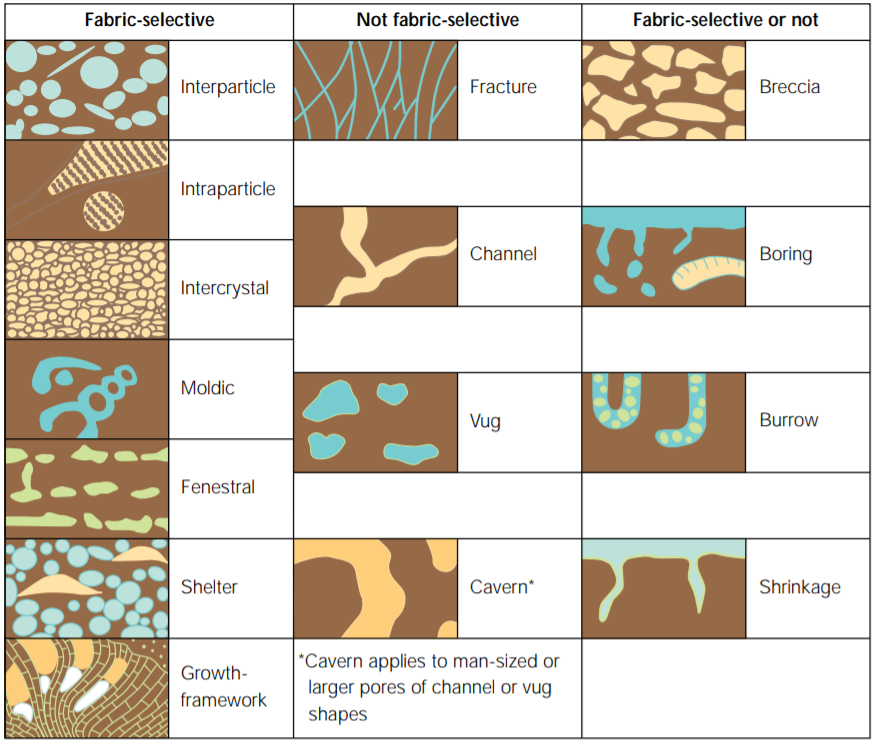
\includegraphics[width=1\textwidth]{\dir/figs/fabricselectivity}
  \caption{Carbonate rock pore classification by fabric selectivity. Left column: Fabric-selective pores. Middle column: Non-fabric-selective pores. Right column: possibly frabric-selective pores. Adapt from \citep{akbar1995classic}.}
  \label{fabricselectivity}
\end{figure}

\paragraph{Interparticle and vuggy pores}
\citet{lucia1995rock} developed a carbonate classification , built on his own work in 1983 \citep{lucia1983petrophysical} that taken both fabric selectivity and petrophysical properties into consideration. This classification serves better for reservoir classification because it focuses more on the goal of describing the spatial distribution of petrophysical parameters such as porosity, permeability and fluid saturation. This classification scheme is summarised in Fig.\ref{interparticle} and Fig.\ref{vuggy}. Pores in carbonate rocks are categorised into two main groups, interparticle pore space and the vuggy pore space. The interparticle pore space is divided further into three sub-categories based on size and sorting of grains and crystals, termed rock-fabric/petrophysical classes (Fig.\ref{interparticle} lower). These three classes define permeability and saturation fields and therefore can be used together with other data to relate petrophysical properties with geological observations \citep{lucia1995rock}.The fabrics are divided into grain-dominated fabric and mud-dominated fabric. For the vuggy pore space, two sub-categories are divided based on vug interconnection, namely separate-vug pores and touching-vug pores. The fabrics are divided into grain-dominated, mud-dominated and grain-mud-dominated fabrics (Fig.\ref{vuggy}). \citet{lucia1995rock}'s classification improved Archie's \citep{archie1952classification} by incorporating \citep{choquette1970geologic}'s fabric-selectivity concept.

\begin{figure}[htbp]
  \centering
  \includegraphics[width=.9\textwidth]{\dir/figs/lucia}
  \includegraphics[width=.9\textwidth]{\dir/figs/lucia3}
  \caption{Interparticle pore space from the classification scheme of \citet{lucia1995rock}. Upper figure: Carbonate interparcitle pores categorised into two main groups: 1) grain-dominated fabric and 2) mud-dominated fabric. Further categorised into sub-groups by percentage of interparticle porosity. Lower figure: Petrophysical classes of the upper figure. The upper figure is re-divided into three classes: class 1) grain-dominated grainstone. Class 2) grain-dominated packstone. Class 3) mud dominated packstone/wackestone/mudstone. Adapt from \citep{lucia1995rock}.}
  \label{interparticle}
\end{figure}

\begin{figure}[htbp]
  \centering
  \includegraphics[width=.9\textwidth]{\dir/figs/lucia2}
  \caption{Vuggy pore space from the classification scheme of \citet{lucia1995rock}. Vuggy pore space of carbonate rocks are divided into separate-vug pores and touching-vug pores. Two sub-divisions of separate-vug pores are grain-dominated fabric pores and mud-dominated fabric pores. Image adapted from \citep{lucia1995rock}.}
  \label{vuggy}
\end{figure}

\paragraph{Porosity Distribution Classification}
\citet{lonoy2006making} improved Lucia's classification by introducing the consideration of porosity distribution. L{\o}n{\o}y's classification of carbonate pores is based on three criteria, namely pore type, pore size and pore distribution. Six pore types are defined: Interparticle, intercrystalline, intraparticle, moldic, vuggy and mudstone microporosity. Pore sizes are divided into three categories: micropores, mesopores and macropores. The defined range of the pore size types are dependent on pore types. Pore distribution has two classes, uniform and patchy. Combining these three criteria L{\o}n{\o}y had summarised 20 types of pore fabrics (Fig.\ref{lonoy}).

\begin{figure}[htbp]
  \centering
  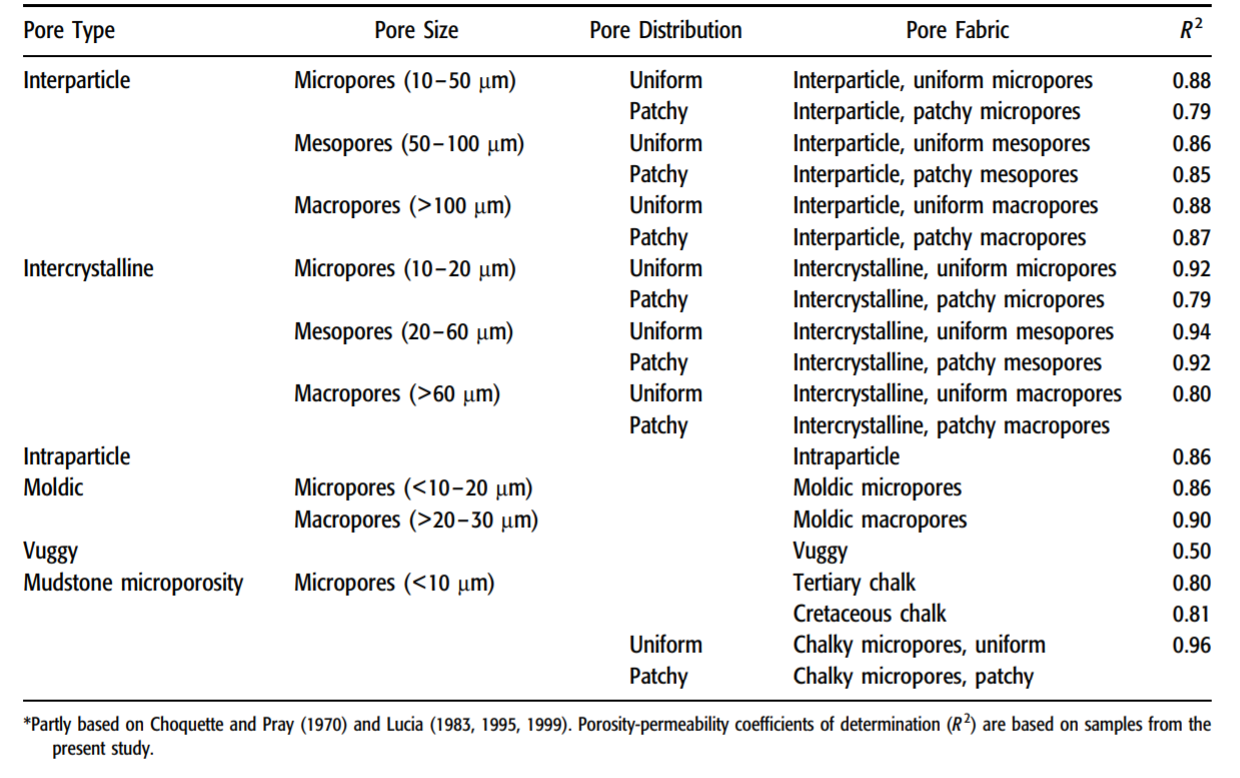
\includegraphics[width=.9\textwidth]{\dir/figs/lonoy2006}
  \caption{L{\o}n{\o}y's classification. Carbonate pores are classified based on pore type, pore size and pore distribution. 20 types of carbonate pore structures are classified. The trend line coefficients of determination $R^2$ of each pore class were significantly improved compared to other classifications, indicating good separability of the classification scheme. Adapted from \citet {lonoy2006making}.}
  \label{lonoy}
\end{figure}

\section{Multiphase flow in porous media}
In this section, basic concepts of multiphase flow in porous media, in a general context, will be introduced. Before discussing multiphase fluid flow, we first consider a porous medium with only one fluid that flows in.

\subsection{Permeability}
The porous medium has an intrinsic property called permeability, it measures the capacity of porous medium to transmit a particular fluid \citep{peters2012overview}. According to the review by \citet{honarpour2018relative}, permeability of a porous medium is defined as following: 

\textit{``A porous material has a permeability of 1 D when a single-phase fluid with a viscosity of 1 cP (10$^-3$ Pa·s) completely saturates the pore space of the medium and will flow through it under viscous flow at the rate of 1 $cm^3/sec/cm^2$ cross-sectional area under a pressure
gradient of 1 atm/cm''} 

Permeability has the units of length squared, which is $m^2$ in SI unit. However conventionally the Darcy (D) is used as the unit for permeability. The Darcy by definition is not based on a conversion to SI units, it is converted to SI unit that $1D \approx 10^{-12} m^2$ with sufficient accuracy for engineering purposes. The Darcy is a very large unit, the more common unit for permeability in rocks is milliDarcy (mD). One reservoir rock with the permeability of below 1 mD is conventionally classified as 'low permeability', 1-10 mD is 'fair permeability' and 10-100 mD will be 'high permeability'.

\subsection{Darcy's law}
When a single phase fluid flows in a porous medium, its flow rate can be described by Darcy's law. French engineer Henry Darcy \citeyear{darcy1856public} first introduced this empirical relationship to describe flow in sand filters for fountains. The flow rate is linked to the viscosity and density of the fluid itself, as well as the permeability of the pore system. The general form of Darcy's law was first proposed by \citet{nutting1930physical} and \citet{wyckoff1933measurement} as:

\begin{equation}
    \mathbf{q}=-\frac{K}{\mu }(\nabla P-\rho \textbf{g})
\end{equation}

\mathbf{q} denotes the Darcy velocity, i.e. the volume of fluid flowing per unit area (both solid and void). K is the permeability of the porous medium.$\nabla$ P is the pressure gradient and \textrho \textbf{g} is the unit weight of the fluid. Darcy's law is essentially the empirical expression of a simplified Navier-Stokes equation that governs fluid flow. The mathematical expression will not be presented here for simplicity but will be introduced later.

\subsection{Interfacial tension, contact angle and wettability}
\subsubsection{Interfacial tension}
We now consider a system of two immiscible fluids contacting with each other, without a porous medium. When two fluid phases stabilised, the fluids adjust their shape to achieve minimum contacting surface area because of interfacial tension. Interfacial tension, \textsigma, is defined as the energy per unit area of the surface between the phases \citep{blunt2017multiphase}. The energy is sourced from penalty of breaking the inter-molecular interactions within each phase and creating a surface instead. The energy is low between two immiscible fluids with similar inter-molecular bonding (e.g. oil and a high-pressure hydrocarbon gas). The energy is high between two immiscible fluids with different inter-molecular bonding (e.g. air and mercury). The physical explanation of interfacial tension is the competing van der Waals inter-molecular forces inside each phase and between the phases \citep{blunt2017multiphase}. The effect of interfacial tension can be observed in nature. For example, ignoring gravity and buoyancy, an air bubble in water is a round sphere when it is stabilised. This is because sphere has the minimum surface area for a fixed volume. 

\subsubsection{Contact angle}
We now consider two contacting immiscible fluid phases on a solid surface. When two fluid phases stabilised, the interface between the two fluids is usually a smooth surface. Fig.\ref{contactangle} shows a conceptual illustration of how a water droplet resides on a solid surface, surrounded by the second fluid phase-air. The interface between water and air forms a surface. The surface has a curvature $\kappa$, and the radius of the curvature $r=\frac{1}{\kappa}$. For less ideal case, the interface can be irregular and consisted of several curvatures.

\begin{figure}[htbp]
  \centering
  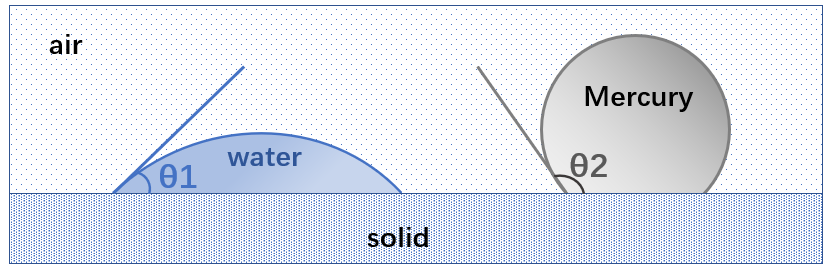
\includegraphics[width=1\textwidth]{\dir/figs/contactangle}
  \caption{Schematic illustration of contact angles measured for a water droplet $\theta 1$ and a mercury droplet $\theta 2$ on a water-wet solid surface (surrounded by air).}
  \label{contactangle}
\end{figure}

At the point where the two fluids are in contact with the solid, an contact angle $\theta$ is formed \ref{contactangle}. The contact angle is dependent on the interfacial tension between the two fluids, and between each fluid and the solid. The contact angle is conventionally measured for the denser fluid phase \citep{blunt2017multiphase}, in this case water, for a valid range from $0^{\circ}$ to $180^{\circ}$. Besides direct measurement, the value of contact angle can be also derived from the Young equation, which will be introduced later.

\subsubsection{Wettability}
From the value of the contact angle, the wettability of the solid can be determined. Wettability indicates the tendency of one fluid phase to spread over the solid surface in presence of another fluid \citep{craig1971reservoir}. In the context of this study, the two fluids are oil and brine, if more generically organic phase, aqueous phase or gaseous phases are concerned for wettability. The contact angle is measured through the water phase because of higher density. If the contact angle $0^{\circ}<\theta<90^{\circ}$, the solid material is water-wet. If the contact angle $\theta=90^{\circ}$, the solid material is neutrally/intermediately-wet. If the contact angle $90^{\circ}<\theta<180^{\circ}$, the solid material is oil-wet. For extreme cases, if the contact angle $\theta=0^{\circ}$, the solid is completely water-wet and for $\theta=180^{\circ}$ the solid is completely oil-wet \citep{blunt2017multiphase}. When referring to the wettability of a porous medium, it refers to the contact angle distribution throughout the pore space . 

In practice, in a real porous rock, the wettability is more complex than in theory. The solid surface can not be absolutely flat and smooth but has some degree of irregularity and roughness, and the mineral composition can be different from place to place. There may be presence of a surfactant in the fluid or deposited on the surface of the solid. The composition of fluids are also complex. In deep aquifers and oilfields, the aqueous phase is a highly saline solution called brine. The composition of a crude oil is even more complex, involving a mixture of hydrocarbon compounds like alkanes, naphthenes and other aromatics and heavy asphaltenes \citep{westlake1974biodegradability}. The fluid wettability might also be altered by soluble gas \citep{lee1974water}. For the above reasons, the wettability in real reservoir/aquifer rock is often non-uniform, wettability can change from pore to pore or even within one single pore.

\citet{mcdougall1995impact} classified the non-uniform wetting systems into two categories. The fractionally-wet system and a mixed-wet system (Fig.\ref{wetsystem}). A fractionally-wet system (Fig.\ref{wetsystem}A) has the wettability distribution of both fluids for all range of pore radius. That is to say, oil-wet pores can be found in all size of pores. A mixed-wet system (Fig.\ref{wetsystem}B) has the wettability distribution that is separated by a specific threshold of pore radius. Pores that are smaller than the threshold radius are water-wet and pores sized above the threshold radius are oil-wet. Such wettability distribution could be a result of wettability alteration which will be discussed later.

\begin{figure}[htbp]
  \centering
  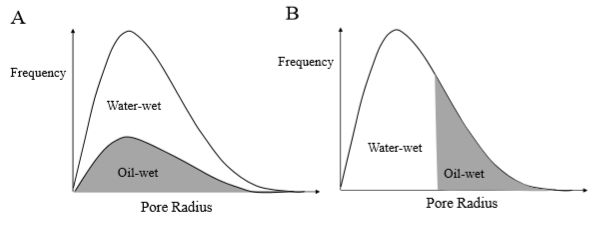
\includegraphics[width=1\textwidth]{\dir/figs/wetsystem}
  \caption{Two wetting systems. For a fractionally-wet system (A), bot oil-wet and water wet pores can both be found in all range of pore radius. For a mixed-wet system (B), water-wet pores and oil-wet pores are separated by a threshold pore radius. Image adapted from \citet{mcdougall1995impact}}
  \label{wetsystem}
\end{figure}

\paragraph{Contact angle hysteresis}
For a stationary fluid droplet on a surface, the contact angle is fixed. However when the fluid droplet is in motion, the contact angle will have different values depending on the direction of motion and wettability. Shown in Fig.\ref{anglehyster}, when the wetting fluid is receding, the receding contact angle $\theta_R$ (1) will decrease compared with the contact angle in equilibrium $\theta_E$ (2). When the wetting phase is advancing, the advancing contact angle $\theta_A$ (3) will increase  compared with $\theta_E$. The difference between advancing and receding contact angles is known as contact angle hysteresis \citep{gao2006contact}. For non-wetting invasion, the displacement is limited by the smallest effective contact angle, the receding angle $\theta_R$. For wetting invasion, the displacement is limited by the largest effective contact angle, the advancing angle $\theta_A$. A pragmatic consequence of contact angle hysteresis is that, when measuring the contact angle (assuming the wetting phase is the denser phase so the contact angle is measured with regard to the wetting phase), the apparent contact angle measured when the fluids are in equilibrium is close to the true contact angle. The contact angle measured during drainage in motion is larger than the true contact angle. The contact angle measured during imbibition in motion is smaller than the true contact angle. There are four reasons for contact angle hysteresis \citep{blunt2017multiphase}: 1) Wettability alteration 2) surface roughness 3) chemical heterogeneity and 4) flow rate.

One pragmatic consequence of the contact angle hysteresis is that, in fast synchrotron experiments which temporal resolution can be around a second, the x-ray imaging may capture both fluid in motion as well as fluid in stagnation. When measuring the contact angles based on such x-ray images, part of the measurements that taken on moving parts of the fluid can be less accurate due to contact angle hysteresis. 

\begin{figure}[htbp]
  \centering
  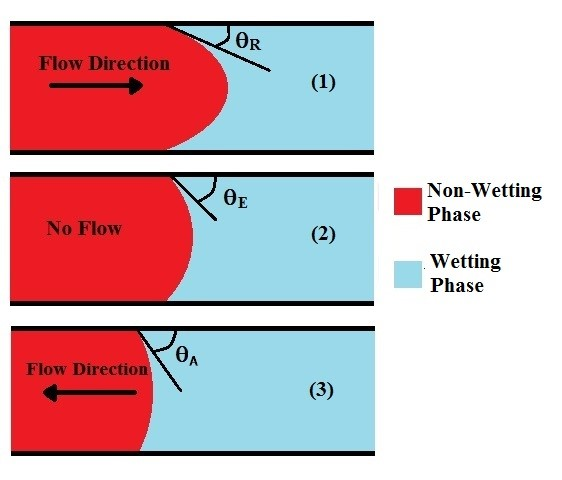
\includegraphics[width=0.7\textwidth]{\dir/figs/anglehyster}
  \caption{Contact angle hysteresis. For contact angle measured in the non-wetting phase (red), the receding contact angle $\theta_R$ that measured at the advancing front is smaller than the genuine contact angle measured at fluid equilibrium $\theta_E$. The advancing contact angle $\theta_A$ that measured on the rear of a moving fluid body is greater than $\theta_E$. Image adapted from \citet{kantzas2012fundamentals}.}
  \label{anglehyster}
\end{figure}

\subsubsection{Wettability alteration}
The wettability of major rock-forming minerals in sedimentary rocks, such as calcite and quartz, is naturally water-wet \citep{abdallah1986fundamentals}. Therefore sedimentary rocks such as sandstone and carbonates, are predominantly water-wet prior to oil migration. However, the wettability of a rock surface can be altered naturally by geological process, due to the deposition of heavy and polar components of the crude oil, such as asphaltenes and resins, on the rock surface. These polar molecules, either acidic-charged or basic-charged \citep{benner1941effect}, can interact with the surface of minerals exposed on the rock surface and therefore alter the wettability in contact \citep{crocker1988wettability}. For core-flooding experiments in the context of oil recovery, it is crucial to conduct experiments in mimic reservoir conditions, including temperature, pressure and wettability. So a process called aging is adopted to artificially alter the wettability of a "clean" rock sample to simulate the wettability condition in reservoir. Aging is a crucial method in core analysis studies and has been increasingly used and discussed in related studies \cite{anderson1986wettability,al2005wettability,kowalewski2003wettability}. 
\paragraph{Wettability alteration in reservoir}
For a typical oil reservoir, the reservoir rock was saturated with an aqueous phase - reservoir brine prior to oil migration. When oil migrated into the reservoir, it entered as the non-wetting phase, while the brine stayed close to the rock surface. As oil migration proceeded, oil replaced the brine in place and left behind an irreducible brine saturation. The residual brine, as the wetting fluid, resided as thin brine films coating the rock surface, and resided as thin layers in the corners, throats, roughness and narrow crevices of the pore space, while oil occupying the pore centres. Crude oil can alter the adjacent rock surface in two ways: by diffusion of polar molecules through the brine film \citep{cuiec1984rock,anderson1986wettability}, or by direct reaction with the surface by brine film collapse \citep{hirasaki1991wettability,buckley1996mechanisms}.

As in one single pore both wetting and non-wetting fluid can co-exist because of the crevices that allow wetting fluid to persist, and different fluid configuration in a single pore can result in different wettability alteration patterns in that pore. \citet{kovscek1993pore} discussed two phase fluid configuration in star-shaped pore and the wettability pattern. \citet{hui2000effects} discussed three phase fluid configuration in triangle-shaped pore and the wettability pattern. These discussions are very important because the wettability alteration in a single pore is non-uniform due to the existence of brine film and wetting corners. This results in non-uniform wettability of single pore \ref{wetconfig}:

\begin{figure}[htbp]
  \centering
  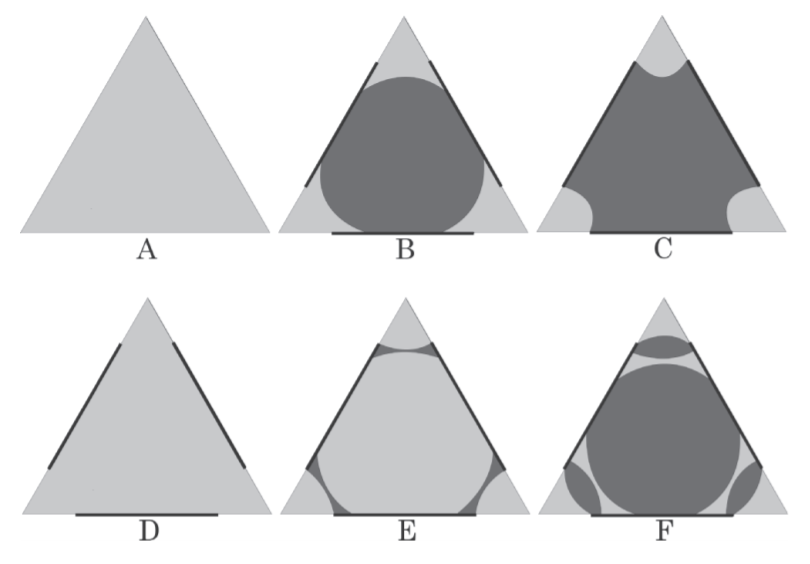
\includegraphics[width=1\textwidth]{\dir/figs/wettabilityconfig}
  \caption{Possible fluid configurations for water (blue) and oil (red) in wettability-altered triangle-shaped pore cross-section. Bold line indicates altered surface wettability. A: water-wet unaltered pore. B: pore body altered to less water-wet. C: pore body altered to oil-wet. D: pore body altered but still strongly water wet. E: Oil only exist as thin layer between corner flow and main water body, therefore only the contacting surface became oil-wet. F: the combination of B and E, but the contacting surface altered to only slightly water-wet. Modified from \citet{helland2006physically}}
  \label{wetconfig}
\end{figure}

\paragraph{Wettability alteration in laboratory}
In the laboratory the aim of wettability alteration is to establish wettability condition that resembles the reservoir \citep{al2005wettability}, because it is one of the major controlling factor of fluid flow. To achieve this, aging is conducted at simulated reservoir condition, including temperature, pressure, connate brine saturation and composition and crude composition. 

The initial step of aging is saturating the cleaned sample core plug with brine. Then crude oil is introduced into the porosity by injection or centrifugation to replace the brine until representative initial water saturation is achieved. The residual brine is assumed to form thin films that has two crucial impacts, first determine the pattern of wettability alteration inside the pores, second take part and assist in the aging process \citep{buckley1996mechanisms}. The aging process lasts for many weeks at reservoir temperature and pressure.

\citet{Pak2014thesis} reviewed a number of studies that identified the main controlling factors for wettability alteration. The main factors are 1) crude oil chemical composition, 2) mineralogy (surface charge) of the rock, 3) salinity and composition of the brine and 4) aging time and temperature. The factors are listed as an overview but will not further discussed because they are beyond the scope of this thesis.


\subsection{Capillary pressure}
When two fluids present in a porous medium, each fluid exerts pressure at the interface of the two fluids. The difference in pressure of the two fluids at the fluid interface is defined as local capillary pressure.

The simplest demonstration of capillary pressure is the capillary rise experiment \citep{young1805iii,leverett1941capillary} in which capillary pressure can be directly visualised. In a capillary rise experiment, the porous medium is of its simplest form - cylindrical tube(s). And the fluids are usually liquid (water, mercury) and gas (air).

Figure \ref{capillaryrise} shows a conceptual illustration of a capillary rise experiment. For a water-air system (a), water is the wetting fluid, the capillary pressure on the fluid interface works against the atmospheric pressure and gravitational force, resulting in a rise of water column by distance $h$ in the tube. For a mercury-air system (b), air is the wetting fluid. The net effect of capillary pressure, atmospheric pressure and gravitational force is a drop of mercury in the tube. 

For a cylindrical tube of diameter $d$, with two fluids of contact angle \texttheta. Given the interfacial tension \textsigma of the two fluids, capillary pressure at the fluid interface can be calculated using the below equation:

\begin{equation}\label{pc}
    P_c=\frac{2\sigma cos \theta}{r}
\end{equation}

This equation stated that, for a interface of two given fluids (thus fixed \textsigma) at a cylindrical pore throat, the local capillary pressure is proportional to the contact angle, and inversely proportional to the radius of the throat. This equation is derived from the fundamental Young-Laplace equation which will be discussed in the following section. The equation \ref{pc} also explains the fact that in a porous medium, the wetting fluid tends to first occupy pores and throats of the smallest diameter, then fill larger pores in the order of ascending diameter. It is vice versa for non-wetting fluid, which tends to first occupy the largest pores, and then fill smaller pores in the order of descending diameter.

\begin{figure}[htbp]
  \centering
  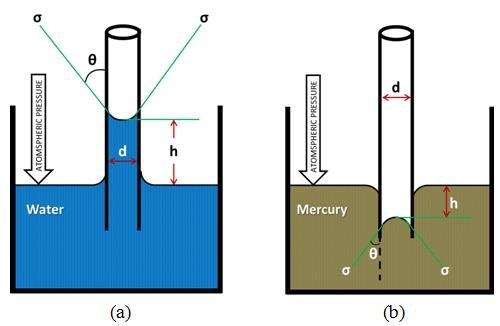
\includegraphics[width=1\textwidth]{\dir/figs/Capillaryrise}
  \caption{Conceptual capillary rise experiment. The tube (diameter $d$) is water-wet, when the tube is immersed in water (a), the vertical component of the capillary force ($\sigma$) works against atmospheric pressure and gravity, caused a rise $h$ of the water body. When the fluid is mercury (b), the contact angle caused the capillary force pointing $\sigma$ downwards. the vertical component of $\sigma$ work along with atmospheric pressure and gravity, caused a drop $h$ of the mercury body. Adapt from \citet{kerimov2014middle}.}
  \label{capillaryrise}
\end{figure}

The fundamental difference of capillary pressure of the wetting and non-wetting fluids categorises fluid flow into two domains: imbibition and drainage. Imbibition refers to the process of a wetting-fluid displacing a non-wetting fluid, and drainage refers to the process of a non-wetting fluid displacing a wetting fluid (Fig.\ref{drainandimbib}). The term imbibition can be easily conceptualised as the process of imbibe water (or any other wetting fluids) in a water-wet medium, and drainage as the process of drain the water by air (or any other non-wetting fluids).

\begin{figure}[htbp]
  \centering
  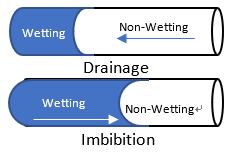
\includegraphics[width=0.7\textwidth]{\dir/figs/drainandimbib}
  \caption{Drainage and imbibition. Drainage is the process of non-wetting fluid displacing wetting fluid. Imbibition is wetting fluid displacing non-wetting fluid}
  \label{drainandimbib}
\end{figure}

\subsection{Drainage}
For a porous medium containing two immiscible fluids, the capillary pressure increases where the pore radius decreases. This means when fluids flow in a porous medium there is a pressure gradient. Fluids flow from high pressure to low pressure, so in drainage process, it is the narrowest restrictions that limit the non-wetting fluid movement.

\subsubsection{Primary drainage}
As mentioned before, the majority of natural rocks are water-wet prior to oil migration, and is entirely saturated with the wetting phase. The first time a non-wetting phase enters the system, this is a primary drainage process. Some common examples of primary drainage in natural systems are \citep{blunt2017multiphase}: the migration of hydrocarbons (liquid or gas) from source rock to a reservoir, the injection of $CO_2$ into a saline aquifer and the process of mercury injection capillary pressure (MICP) for the measurement of pore-size distribution.

During drainage, to enter a pore, the non-wetting fluid must overcome the threshold capillary pressure governed by the locally smallest throat radius $r_t$. The interface between the moving front of the non-wetting fluid and the receding non-wetting phase is called a terminal meniscus (TM) shown in Fig.\ref{tm}. The terminal meniscus can be experimentally identified observed by a distinctive curvature distribution \citep{andrew2015imaging}.

\begin{figure}[htbp]
  \centering
  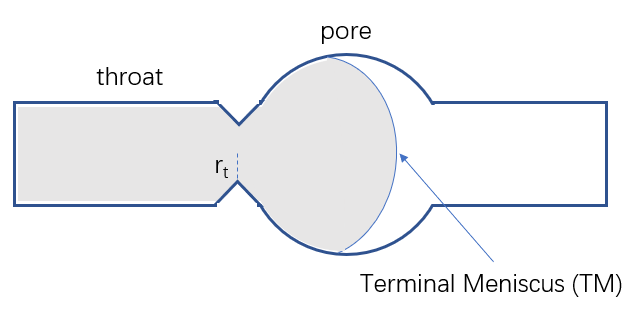
\includegraphics[width=0.6\textwidth]{\dir/figs/tm}
  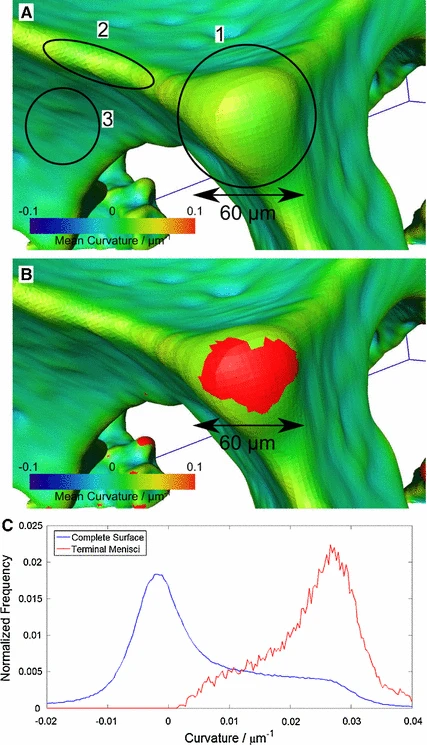
\includegraphics[width=0.6\textwidth]{\dir/figs/terminalmeniscus}
  \caption{Terminal meniscus. The uppermost figure shows the terminal meniscus span across the widest place of a pore in 2D section. The next three figures (A,B,C) are adapted from \citet{andrew2015imaging}. A shows 3D visualisation of a terminal meniscus (circle 1) formed by the fluid (green). B shows curvature measurement on the fluid surface mesh. C shows distinct curvature distribution of the terminal meniscus and the complete surface.}
  \label{tm}
\end{figure}

\subsubsection{Wetting layers}
During drainage, the non-wetting fluid movement is impeded by the narrowest pore throats. Since the pore geometry in a real rock is highly irregular, the wetting phase can reside in the crevices and corners of the pore space. These narrow regions have very high capillary entry pressure thus the wetting fluid inside can not be removed by the non-wetting fluid. These retained wetting fluid can be widely connected throughout the pore network, and are known as wetting layers. Wetting layers are experimentally verified both in 2D and 3D \citep{datta2014mobilization, andrew2015imaging}. Wetting layers have different flow properties than wetting films \citep{blunt2017multiphase}. Wetting films cover the surface of the solid, their thickness is molecular-scale and does not support significant fluid flow. In contrast, wetting layers that reside in the crevices and corners are of macroscopic (few microns) thickness and therefore allow appreciable flow movement.

\begin{figure}[htbp]
  \centering
  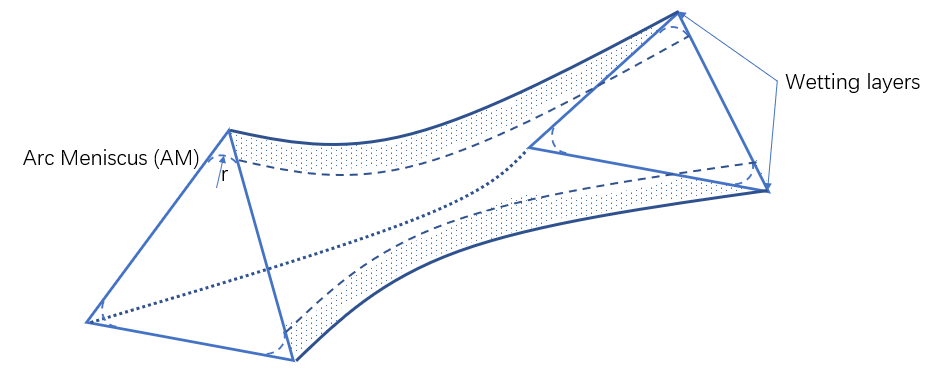
\includegraphics[width=0.9\textwidth]{\dir/figs/wl}
  \caption{Wetting layers and arc meniscus. For a pore system with corners (simplified as a triangle-shaped cross section), thus allowing corner flow, wetting layers can exist in the corners and connect throughout many pores in the system. The curvature (radius $r$) of the wetting layer forms the arc meniscus. Redrawn from \citet{blunt2017multiphase}}
  \label{wl}
\end{figure}

Fig.\ref{wl} demonstrates the conceptual fluid configuration of wetting layers in a simplified pore throat. The wetting layers are crucial structures for fluid flow in porous media, because they allow wetting fluid flow throughout the pore network even at high non-wetting saturation, and allow the important mechanism of snap-off to occur during imbibition.

\subsubsection{Haines jumps}
During drainage, the non-wetting fluid will retract from regions of high pressure and move towards low pressure following the pressure gradient. The local pressure gradient leads to a rapid filling, regardless of the slowness of external rate of injection, of a series of wider pores in order to achieve capillary equilibrium. Meanwhile, the non-wetting fluid retracts from regions of high pressure to allow the filling of low pressure regions.

This process of fluid rapidly filling multiple pores is called Haines jumps \citep{haines1930studies}, firstly discovered in soil moisture studies. Different from the gradual filling of a pore which can be filled by a smooth reversible process, Haines jumps are quantised, meaning that the pores are filled by Haines jumps by an irreversible, instantaneous process. Capillary equilibrium can only be established before and after the jumps, but the jump process is unstable, therefore there is no half-filled pore by Haines jumps.

In the core flooding experiments by \citet{berg2013real}, they correlated small pore pressure fluctuations with multiple fast pore filling events seen before and after in scans. The finding changed the common singular pore jump paradigm of Haines jumps. One Haines jump typically cascade through 10-20 geometrically defined pores. Fig.\ref{hj} shows Haines jump events of different scale imaged by synchrotron microtomography \citep{berg2013real}. The upper row of images shows a large scale Haines jump event that affected several connected pores. The bottom row shows a small scale Haines jump event that filled single pore. These events were proved genuine by pressure records.

\begin{figure}[htbp]
  \centering
  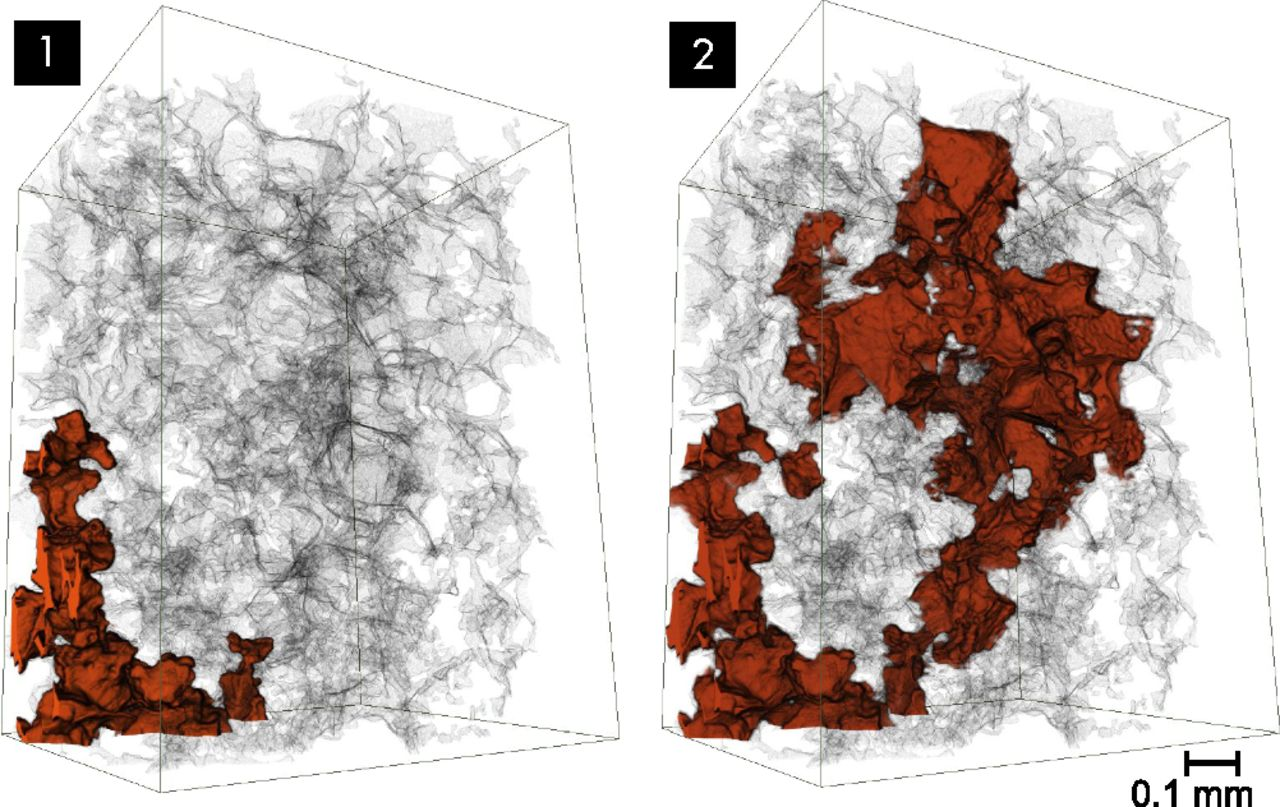
\includegraphics[width=0.9\textwidth]{\dir/figs/hjlarge}
  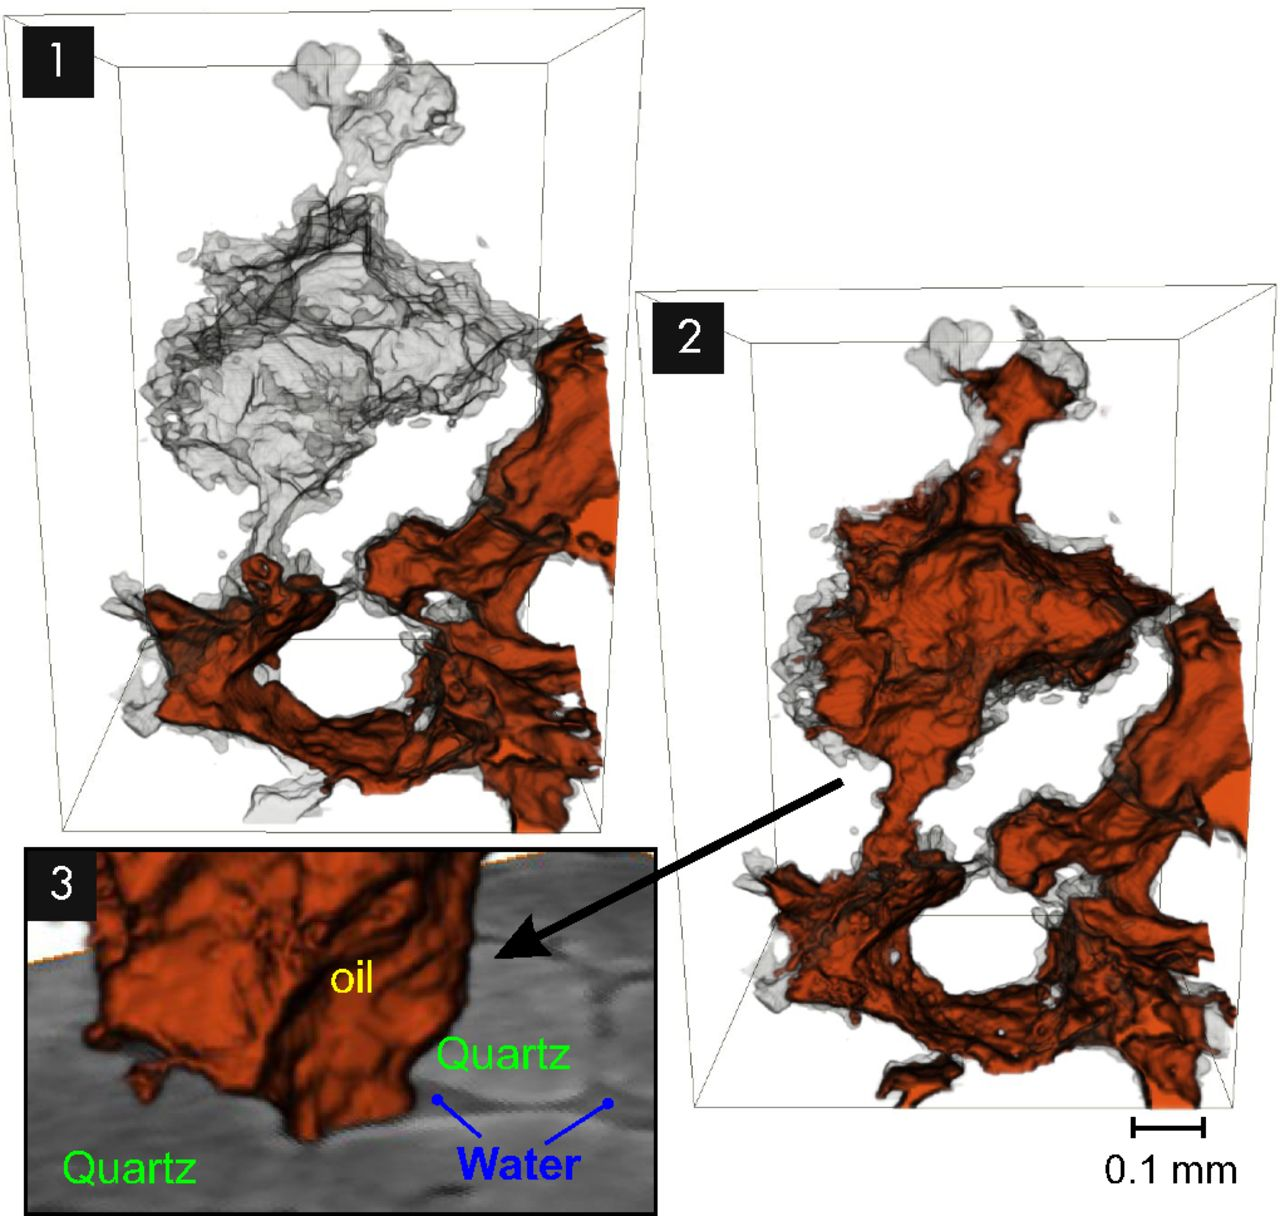
\includegraphics[width=0.9\textwidth]{\dir/figs/hjsmall}
  \caption{Haines jumps of different scales. The upper two images shows a large scale Haines jump (timestamp 1-2) of oil that span across 10+ pores. The lower three images shows a small scale Haines jump (timestamp 1-2) that only affect one pore. 3 is the zoomed-in image that shows the oil, water and rock phase corresponding to the 2D CT reconstruction image. Adapt from \citet{berg2013real}.}
  \label{hj}
\end{figure}

A Haines-jump event involves fast filling of multiple pores, and consequently the retraction and snap-off of the non-wetting phase at higher-pressure regions. Importantly, the retraction of non-wetting phase can be non-local, i.e. can occur throughout the system. Such retraction is a local imbibition process in a drainage event. \citet{andrew2015imaging} imaged a Haines-jump event of super-critical $CO_2$ displacing brine in Ketton limestone during primary drainage. The captured Haines-jump event resulted in the retraction and snap-off of the non-wetting phase that is distal and indirectly involved with the Haines-jump event (Fig.\ref{distalretraction}).

\begin{figure}[htbp]
  \centering
  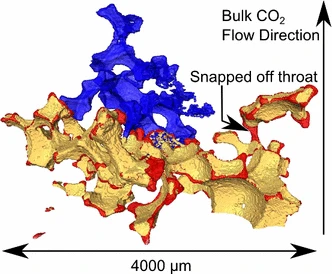
\includegraphics[width=0.75\textwidth]{\dir/figs/distalretraction}
  \caption{Haines jump can cause retraction of the non-wetting fluid, even at a distance from the pore where Haines jump occurs. Yellow is the non-wetting fluid $CO_2$. Blue is the Haines jump event. Red shows the retraction of $CO_2$ after the Haines jump event. A distal snap-off event (notation with arrow) happened few pores away from the Haines jump event. Image adapt from \citet{andrew2015imaging}.}
  \label{distalretraction}
\end{figure}

\subsubsection{Roof snap-off}
Haines jumps are associated with one important mechanism called Roof snap-off. It is a phenomenon that when non-wetting fluid emerge from a throat into a pore, the capillary pressure is in favour of separating the leading portion of the non-wetting fluid into droplets (Roof snap-off), and rapidly fill the adjacent pore in an irreversible Haines jump-fashion. Roof snap-off is firstly directly observed by \citet{roof1970snap} during drainage in an idealised pore geometry. A simplified diagram of a Roof snap-off event is shown in Fig.\ref{roofdemo}.

In Fig.\ref{roofdemo} upper figure, shows the critical radius of the terminal meniscus $r_{crit}$ being reached by the invading non-wetting fluid. This is the critical onset moment of a Roof snap-off event. After the critical radius of the $r_{crit}$ has been reached (middle figure), the surface tension is in favour of splitting the moving front of the non-wetting fluid into a droplet. This is the ongoing moment of a Roof snap-off event, while snap-off in imbibition requires thickening of wetting layers, Roof-snap off can occur without wetting layers but through thin film flow \citep{roof1970snap, gauglitz1990dynamics}. The fluid interface will rapidly recover to the smallest to minimise the surface energy. The Roof snap-off can happen several times, rapidly, until the adjacent pore is completely filled by the non-wetting phase (bottom figure). The non-wetting fluid in the throat will retract and form new terminal meniscus with a radius of curvature $r$. The new capillary equilibrium will be lower than pre-snap-off, indicated by $r>r_{crit}$. At the end of the event, the pore is end with a trapped non-wetting ganglion (blob) in the pore space (bottom figure). The trapped ganglion can be reconnected once the throat filled by more incoming non-wetting fluid.

\begin{figure}[htbp]
  \centering
  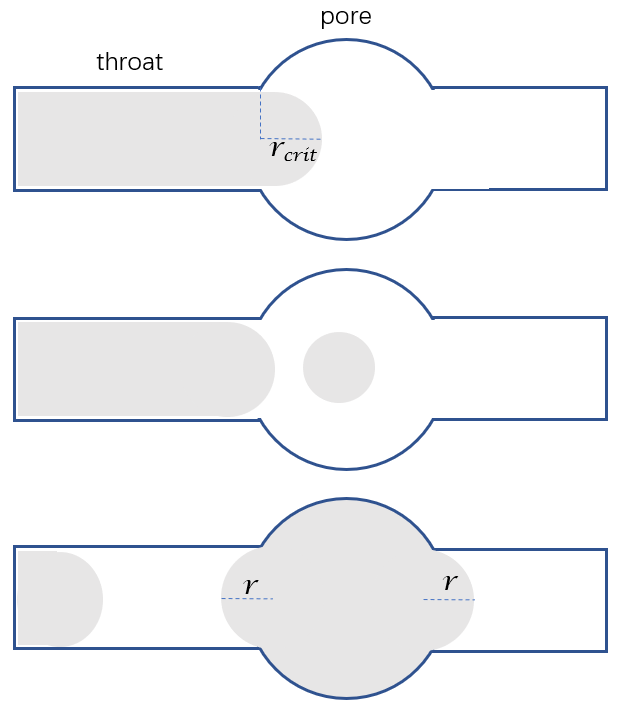
\includegraphics[width=0.7\textwidth]{\dir/figs/roofdemo}
  \caption{Conceptual Roof snap-off in a 2D pore section. The top figure shows the onset of a Roof snap-off event, the non-wetting fluid enters the pore and reached a critical radius $r_{crit}$. The middle figure shows the ongoing Roof snap-off that the front of the non-wetting fluid is snapped-off. The bottom figure shows that once the snap-off began, the pore will be rapidly filled by repeating snap-off. The new equilibrium is reached when the pore is completely filled, and disconnected with its feeding body.}
  \label{roofdemo}
\end{figure}

\subsection{Imbibition}
Imbibition is the reverse process to drainage, i.e. the process of a wetting fluid displacing the non wetting fluid. Capillary pressure by definition is the difference of non-wetting and wetting phase. During imbibition the wetting fluid saturation is increased therefore the capillary pressure in the system is decreased. 

Imbibition examples in nature can be soaking of water into soil and absorption of water into dry woods etc. The first entry of the wetting fluid into a porous medium is primary imbibition, for example the filling of dry sand by water. After primary drainage, the pore space is mostly saturated with non-wetting phase, but wetting phase can still exist in the form of wetting films and wetting layers. In this case, the re-entry of wetting fluid is secondary imbibition \citep{blunt2017multiphase}. The example of secondary imbibition can be water-flooding an oil reservoir (if the reservoir rock is water-wet).

There are two type of processes that occur during imbibition: snap-off and piston-like advance. The imbibition process is ultimately controlled by the competition of snap-off and piston-like advance (Fig.\ref{pistonandsnappoff}). These two important processes will be introduced in the following sections.

\begin{figure}[htbp]
  \centering
  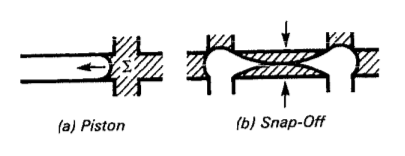
\includegraphics[width=1\textwidth]{\dir/figs/pistonandsnapoff}
  \caption{Two major filling mechanisms in imbibition. (a) Piston-like advance which wetting fluid displacing non-wetting fluid in a piston-like motion. (b) Snap off, wetting films can bulge or swell and eventually merge to fill a previously non-wetting occupied throat. Adapt from \citet{lenormand1984role}.}
  \label{pistonandsnappoff}
\end{figure}

\subsubsection{Piston-like advance}
Piston-like advance is the direct filling of pore space by wetting fluid. Wetting fluid during piston-like advance has a rather flat front and leaves very little non-wetting fluid trapped behind (Fig.\ref{pistonandsnappoff} (a)). The presence of wetting layers is crucial for spontaneous filling of the wetting phase in piston-like advance, it is theoretically proven that the wetting layers make the throat appear more water-wet than without them \citep{ma1996effect,oren1998extending}.

\subsubsection{Cooperative pore filling}
During imbibition the capillary pressure is always decreased, therefore the wetting fluid will preferentially fill throats rather than pores. That is to say, in contrast with drainage that is impeded by throats, the imbibition process is impeded by pores. The pore filling criterion for imbibition is governed by capillary entry pressure which is decided by the largest curvature radius of the terminal meniscus. To decide the critical curvature radius in one particular pore, we have to not only consider the size and shape of the pore, but also consider the wetting fluid saturation of the bounding throats of that pore. If the filling of a pore is assisted by wetting fluid in the bounding throats, then this is cooperative pore filling in imbibition.

Firstly discussed by \citet{lenormand1983mechanisms,  lenormand1984role}, the cooperative pore filling mechanism is named $I_n$, where n is the number of bounding throats that filled by non-wetting fluid. For example if a pore has one adjacent throat that filled by non-wetting fluid, this is an $I_1$ cooperative pore filling process.

\begin{figure}[htbp]
  \centering
  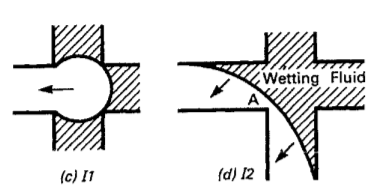
\includegraphics[width=1\textwidth]{\dir/figs/i1i2}
  \caption{Cooperative pore filling event $I_1$ and $I_2$. $I_1$ shows when only one adjacent throat is filled by non-wetting fluid. $I_2$ is when two of the adjacent throats are filled by non-wetting fluid. The critical radius of the curvature $I_1$ is smaller than $I_2$ therefore an $I_1$ event is more preferred to happen than $I_2$ while both events are possible. Adapt from \citet{lenormand1984role}.}
  \label{i1i2}
\end{figure}

First we look at an $I_1$ process (Fig.\ref{i1i2} left). This denotes an $I_1$ process because the pore has only one adjacent throat that is filled by non-wetting fluid. The largest curvature radius of the terminal meniscus is the radius of the circle in the middle which is also the pore radius. An $I_2$ process (Fig.\ref{i1i2} right) is where two of the adjacent throats are filled by non-wetting fluid. I2 has much larger curvature radius of the TM, thus is less favoured by the wetting fluid. 

$I_3$ and higher $n$ processes are rarely seen \citep{blunt2017multiphase}, and it is theoretically demonstrated that higher $n$ events are less favoured by the imbibition process \citep{blunt1998physically,oren1998extending}. A simulation was done in a Bentheimer sandstone pore network model to quantify the frequency of events in imbibition \citep{blunt2017multiphase}, and the result agreed with the theoretical implication that higher $n$ events are less frequent.

One important feature of cooperative pore filling in imbibition is that theoretically it leads to a flat frontal advance with no trapping \citep{blunt1992simulation}. In the simulation the wetting phase displaced the non-wetting phase by a cycle of $I_3$ - $I_2$ events therefore leading to a flat frontal advance with no trapping (Fig.\ref{frontadvance}.

\begin{figure}[htbp]
  \centering
  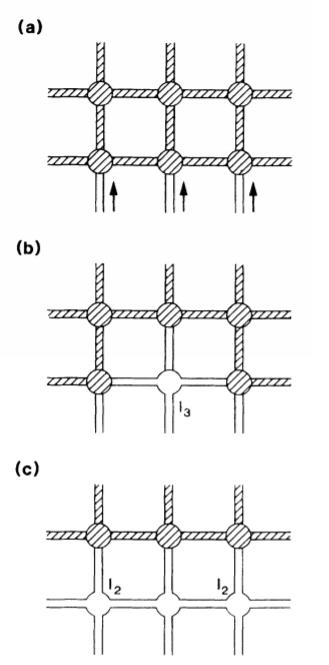
\includegraphics[width=0.5\textwidth]{\dir/figs/frontaladvance}
  \caption{Flat frontal advance associated with cooperative pore filling in imbibition, in a pore system with relatively homogeneous pore size distribution. Dashed line stands for non-wetting fluid and blank stands for wetting fluid. Arrow is the direction of the flow. (a) shows three pores that are all potentially $I_3$ filling events, chances are equal that one of the pore can be filled by an $I_3$ event. (b) When one of the pore is filled by an $I_3$ event, the filling of the rest two pores became two potential $I_2$ events. Because $I_2$ is more preferable than $I_3$, the rest two pores will be filled rather than going for another $I_3$ event. (c) When the rest two pores were filled by two $I_2$ events, it becomes the same situation as (a) where three potential pores are all $I_3$ events. This filling cycle will lead to a flat frontal advance with no trapping left behind. Image adapt from \citet{blunt1992simulation}.}
  \label{frontadvance}
\end{figure}

\subsubsection{Wetting layer swelling and snap-off}
In imbibition, the swelling of wetting layers leads to snap-off (Fig.\ref{pistonandsnappoff} (b)). Snap-off was first described by \citet{pickell1966application}. It occurs in the narrowest region of the throats, leading to partial filling of the two adjacent pores. A demonstration of the wetting layer swelling and snap-off is drawn as Fig.\ref{snapoffdemo}.

During imbibition, the wetting phase can flow in the wetting layers and therefore increase their thickness. Before a snap-off event, the wetting layers keep swelling until they meet. The swelled wetting layers are most easily met at the narrowest region of the throat, and this is when snap-off begins. Two terminal menisci that curved towards opposite direction are formed where the wetting layers met. The entire throat will be rapidly filled by the wetting fluid once snap-off occurs, consequently the two terminal menisci will retreat to a critical radius that allows new capillary equilibrium to establish.

\begin{figure}[htbp]
  \centering
  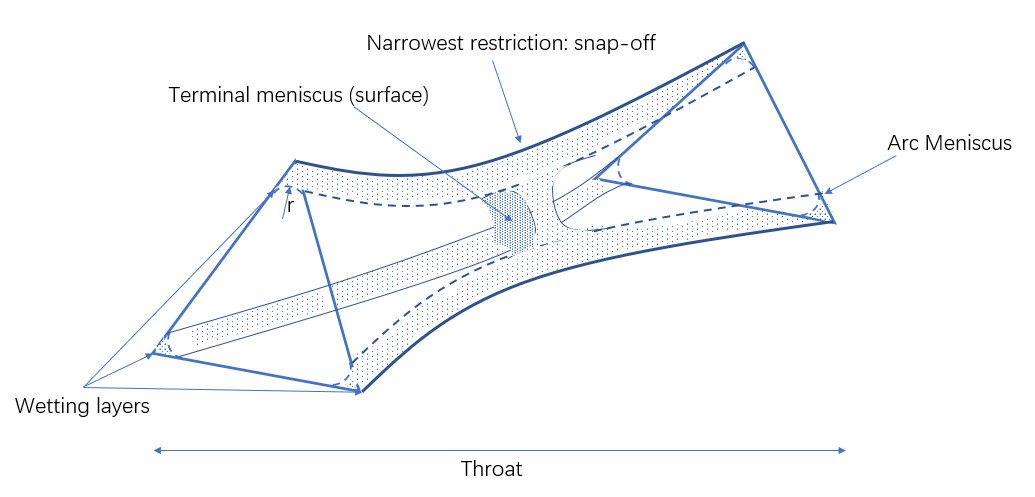
\includegraphics[width=1\textwidth]{\dir/figs/snapoffdemo}
  \caption{Snap-off illustrated in a simplified throat. The wetting layers allows wetting fluids flow in corners and crevices while non-wetting fluid occupying the centre of the throat. During imbibition, wetting layers can swell and easily merge at the narrowest point of the throat, causing snap-off of the existing non-wetting fluid and eventually fill the entire throat. Redrawn from \citet{blunt2017multiphase}}
  \label{snapoffdemo}
\end{figure}

\subsubsection{Displacement patterns in imbibition}
The competition between snap-off and piston-like advance forms four generic types of displacement patterns in imbibition \citep{chandler1982capillary,lenormand1984role,cieplak1988dynamical,cieplak1990influence}: 1) percolation with trapping, 2) invasion percolation, 3) frontal advance and 4) cluster growth. The term percolation comes from the approach of representing a porous medium using a network model. The pores and throats were analogous to 'sites' and 'bonds' of a percolation process \citep{broadbent1957percolation}.

The first type of pattern is percolation with trapping. In a heterogeneous porous medium that allows flow in wetting layers, pores and throats are filled in order of size. Flow in wetting layers are connected throughout the pore system so that imbibition can take place anywhere in the system. Non-wetting phase can be trapped by snap-off events. This is the most commonly encountered case in reservoir settings \citep{blunt2017multiphase}.

The second type invasion percolation is similar to the first type, but without flow in wetting layers (for example primary imbibition into a dry rock). This results in limited choice of pore-filling that does not purely dependent on order of size, but also the accessibility of fluids. 

The third type flat frontal advance is more common in less heterogeneous medium, where cooperative pore-filling is in dominance. The advancing front of the wetting fluid is flat due to the repetition of $I_n$ processes (Fig.\ref{frontadvance}. Non-wetting fluid is rarely trapped. An example of this type of displacement is paper towel soaking water. 

Cluster growth is similar wit frontal advance, but crevice flow exists. Wetting layers allow fluid to access any pore in the system, therefore pore-filling can happen distance away from inlet. Instead of flat frontal advance from the inlet, in this type of imbibition pores are filled as growing clusters inside the porous medium and left almost no trapped non-wetting phase. This type could occur in a pore system where the pores and throats are of similar size \citep{blunt2017multiphase}.

\subsection{Relative permeability}
\paragraph{Relative permeability definition}
The permeability introduced at the beginning of this section is also known as absolute permeability, and is only valid for a porous medium that is completely saturated by the measured flowing fluid \citep{honarpour2018relative}. For immiscible multiphase fluid flow, the more useful representation of permeability is effective permeability which for each fluid is a function of its percentage saturation.

Relative permeability is defined as the dimensionless ratio of effective permeability to absolute permeability. For two phase flow of oil and water, the relative permeability of oil and water is noted as $k_{ro}$ and $k_{rw}$ respectively. The general shape of $k_{ro}$ and $k_rw$ can be approximately represented by $k_{rw}=A(S_w)^n$, $k_{ro}=B(1-S_w)^m$ where $S_w$ is the saturation of water and A,B,m,n are constants.

\paragraph{Relative permeability during drainage and imbibition}
Assuming a water-wet porous rock that initially saturated with 100\% water. At this time $k_{rw}=1$ and $k_{ro}=0$. During primary drainage, the oil first traverses through the largest pores, resulted in disconnecting the most conductive paths (narrow throats) for water therefore $k_{rw}$ drops rapidly. Meanwhile as oil saturation increases and more oil pathways are established, $k_{ro}$ will rise. $k_{ro}$ and $k_{rw}$ curves will eventually cross as drainage continues, the water saturation of the crossing point will vary in different rocks. Because the increase of $k_{ro}$ and the decrease of $k_{rw}$ follow a power law, the relative permeability for both fluids at the crossing point is much less than 0.5, and so the sum of the relative permeabilities of the two fluids is then much less than 1. This means that the total flow of both fluids are impeded \citep{blunt2017multiphase}.

At some point when the oil saturation is high enough for oil to become well connected, the $k_{ro}$ will rise sharply approaching 1. At this time water has reached an irreducible saturation and only exists in form of wetting layers and wetting films. $S_w$ and $k_{rw}$ approach a very low value. 

Relative permeability during secondary imbibition is not the reverse process of primary drainage, because for that the non-wetting phase can be trapped by snap-off events. During secondary imbibition snap-off can disconnect oil pathways with little change in water saturation, leading to a sharp drop of $k_{ro}$ \citep{blunt2017multiphase}. The irreversibility of $k_{ro}$ is also known as hysteresis. It mainly has two causes \citep{spiteri2005relative} 1) contact angle hysteresis. In imbibition there are three ways for water to displace oil: piston-like advance, snap-off and cooperative filling. All three displacement mechanisms are strongly dependent on the wettability, therefore the contact angle hysteresis that changes the intrinsic contact angle to the advancing contact angle leads to change in apparent wettability and resulted in change in displacement mechanism, and ultimately leads to relative permeability hysteresis. 2) trapping of the non-wetting phase. Once the non-wetting phase is trapped by snap-off events, $k_{ro}$ will have a significant drop due to disconnected oil path, and consequently causes relative permeability hysteresis.

The relative permeability of water $k_{rw}$ does not have hysteresis \citep{blunt2017multiphase}. For that water can not be completely trapped therefore has similar conductance for similar saturation, regardless of the displacement process. 

\subsection{Capillary number and flow regime}
Permeability, as previously discussed, is an intrinsic property that as a function only of the pore geometry. This is under the assumption that while a fluid is moving, its velocity field does not change with time. However when the flow rate is high that viscous forces (the friction inside a fluid) become significant enough to cause changes to the velocity field, it consequently alters the microscopic configuration of fluid. Furthermore, it makes relative permeability dependent on Darcy velocity, and challenges the inherent assumption of the multiphase extension of Darcy's law \citep{blunt2017multiphase}. Therefore the impact of flow rate needs to be discussed in order to characterise flow in porous medium. First of all, rather than treating viscous forces and capillary forces separately, a dimensionless capillary number $Ca$ is introduced to represent the net effect of viscous forces and capillary forces between two immiscible fluids:

\begin{equation}
    Ca= \frac{\mu q}{\sigma}
\end{equation}

where $q$ is the Darcy velocity of the flowing fluid, $\mu$ is its viscosity and $\sigma$ is the interfacial tension between two fluids. However, $Ca$ does not represent the ratio of viscous to capillary effects at pore scale directly, it needs to be multiplied by a geometry-saturation-dependent quantity (much larger than 1) to find the true ratio \citep{blunt2017multiphase}. When $Ca \ll 1$, conventionally $Ca<10^{-6}$ \citep{blunt2017multiphase}, the flow is roughly reckoned as dominated by capillary forces. For $Ca>10^{-6}$, viscous effects are significant enough to perturb the fluid configurations, as contact angle has negligible impact on the flow behaviour. To discuss the impact of flow rate on fluid displacement, a classical micro-model experiment by \citet{lenormand1984role} is taken as an example (Fig.\ref{lenormand}). 

\begin{figure}[htbp]
  \centering
  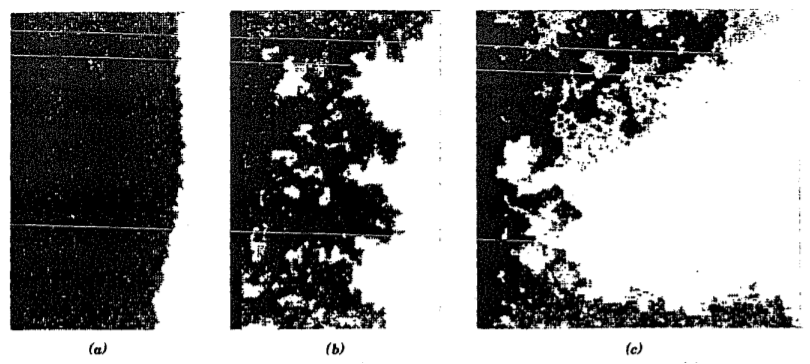
\includegraphics[width=0.8\textwidth]{\dir/figs/lenormand1984}
  \caption{Lenormand's imbibition experiment in a micro model with different flow rate. The micro model contains 42,000 ducts (throats) with 4mm between junctions (pores). The capillary numbers of (a), (b) and (c) are $3\times10^{-4}, 1.4\times10^{-5}$ and $6\times10^{-7}$ respectively. Difference in flow rate caused significant patterns of displacement. At the lowest flow rate, displacement shows flat frontal advance behaviour, and penetrates least of the model length. At the intermediate flow rate, more snap-off and trapping occured. At the highest flow rate, the displacement is the most heterogeneous and penetrates most of the model length, with a percolation-like displacement pattern. Adapt from \citet{lenormand1984role}.}
  \label{lenormand}
\end{figure}

Fig.\ref{lenormand} shows three images of imbibition at different $Ca$. Black is the invading wetting phase injected from left, white is the non-wetting phase being displaced. The $Ca$ from left to right are of $3\times10^{-4}, 1.4\times10^{-5}$ and $6\times10^{-7}$ respectively. Since the interfacial tension and viscosity of a particular fluid stay constant, the only variable is the Darcy velocity, therefore smaller $Ca$ stands for lower flow rate.

At the lowest flow rate (Fig.\ref{lenormand} (c)), where the configuration of fluid at pore scale was controlled by capillary forces only. This is the familiar scenario that have been discussed in the imbibition section. At this rate, the wetting fluid was able to penetrate through most of the model length. The wetting saturation was higher closer to the inlet. There are numerous of isolated non-wetting clusters of non-wetting fluid (white patches inside black) indicating trapped non-wetting fluids. And there shows isolated wetting phase (black patches inside white), indicating the filling of throats by snap-off events, and showing evidence for flow in wetting layers. This is the percolation-like displacement pattern that the pores were filled largely in order of pore size.

At intermediate flow rate (Fig.\ref{lenormand} (b)), the wetting phase travelled shorter of the model length, but the wetting saturation was more homogeneous. There was significantly less snap-off, and trapped non-wetting phase was significantly larger in size.

At the highest flow rate (Fig.\ref{lenormand} (c)), the total volume of trapped wetting phase was low, and confined to small clusters. And there was none snap-off observed. The advancing front was almost flat and the saturation was homogeneous. Piston-like advance was in dominance.

The experiment demonstrates the flow-rate dependency of fluid displacement patterns in imbibition. \citet{blunt2017multiphase}'s interpretation is that, the wetting fluid conductance is low in wetting layers but high through the centres of the pore space. Since layer flow is slow, it has to be sufficiently low flow rate to provide enough time for lots of snap-off events to happen in order of size. If the flow rate is fast, piston-like advance will suppress snap-off events because they can happen much faster. Piston-like advance is more likely to happen near the inlet due to higher wetting fluid pressure. Similar results were also drawn from three dimensional experiments in glass beads packs \citep{datta2014mobilization}.

\subsubsection{Flow regime}
When capillary forces are in dominance, it is possible to describe the multiphase flow using Darcy's law. When viscous forces are in dominance, the inherent assumption of Darcy's law that the displacement pattern is percolation-like is challenged \citep{blunt2017multiphase}. Flow regime refers to the criteria that Darcy's law can or cannot be employed.

A dimensionless number effective capillary number $Ca_{eff}$ is defined as a function of pore length $l$, capillary number $Ca$, porosity $\phi$, permeability $K$ and Bond number $B$ that refers to the ratio of buoyancy to capillary forces:

\begin{equation}
    Ca_{eff}=(\frac{lCa}{\sqrt{\phi K}}+B)
\end{equation}

When viscous forces are in dominance. The flow patterns are controlled by the viscosity ratio $M=\mu_d/ \mu_i$, which is the ratio between the viscosity of the displaced fluid and the injected fluid. $Ca_{eff}$ and $M$ together define the flow regimes\citep{blunt2017multiphase}:

\paragraph{Capillary regime}
When $M<1$ and $Ca_{eff}<1$; or $M>1$ and $Ca_{eff}<1/M$, multiphase Darcy's law is enabled. The flow is capillary-dominated. Displacement pattern is percolation-like.

\paragraph{Viscous regime}
When $Ca_{eff}>1$, the flow is viscous-dominated, and the use of Darcy's law is affected. If $M<1$, the displacement is stable, frontal advance (e.g.Fig.\ref{lenormand} (c)) will occur. If $M>1$, the displacement is unable and will result in viscous fingering, which refers to the onset and evolution of instability during fluid displacement \citep{homsy1987viscous}. For the extreme when $M \rightarrow \infty$, flow pattern is fractal, called diffusion limited aggregation (DLA \citep{witten1981diffusion}).

\subsection{The Young-Laplace equation and Navier-Stokes equation}
For a system of a porous medium containing two immiscible fluid phases, the flow process in this system is ultimately governed by the conservation of three physical properties: the conservation of interfacial energy between fluids, the conservation of momentum and the conservation of mass \citep{blunt2017multiphase}. The two fundamental equations that describe fluid flow in a porous system, namely the Young-Laplace equation and Navier-stocks equation, are derived from the physical conservations.

\subsubsection{Conservation of energy: the Young-Laplace equation}
Conservation of interfacial energy between fluids, and between fluids and solid, governs the fluid configuration in a pore system at capillary equilibrium, and governs the threshold fluid pressure at which displacement can take place. The conservation of interfacial energy is used to derive the Young-Laplace equation\ref{eqy-l}. 

\begin{equation}\label{eqy-l}
    P_{c}=\sigma(\frac{1}{r_{1}}+\frac{1}{r_{2}})=\kappa \sigma
\end{equation}

where $P_{c}$ (unit $m/Lt^2$, \textpsi ) stands for the local capillary pressure, which is derived from the pressure difference between the non-wetting/wetting fluids $P_{nw}-P_{w}$. $r_{1}$ and $r_{2}$ are the radii of curvature of the two fluids. Interfacial tension, \textsigma, according to definition of \citet{blunt2017multiphase} is \textit{"the energy per unit area of the surface between the phases, or the change in free energy for a change in area $\sigma=dF/dA$"}. $\kappa$ is the total curvature of the interface. The Young-Laplace equation relates the local capillary pressure to a function of the interfacial tension and curvature.

Treating the interfacial tensions as force, when apply a horizontal force balance, the Young equation is obtained:

\begin{equation}\label{eq_young}
    \sigma_{nws}=\sigma_{ws}+\sigma cos \theta
\end{equation}

where $ \sigma_{nws}$ ($N/m$) stands for the interfacial tension between the non-wetting phase and the solid, and $ \sigma_{ws}$ as the interfacial tension between the wetting phase and the solid. The fundamental Young equation is an expression for the relation between contact angle and the interfacial tension between the two fluids and the solid.

This equation involves two important concepts of interfacial tension and contact angle. The contact angle, \texttheta, is the angle of the denser fluid phase between solid and the other phase. Interfacial tension and contact angle will be discussed in detail in the following section.

\subsubsection{Conservation of momentum and mass: the Navier-Stocks equation}
Conservation of momentum leads to the Navier-Stokes equations and their macroscopic counterpart, Darcy's law \citep{darcy1856public}. While conservation of energy deals with stationary state of fluids in capillary equilibrium, conservation of momentum deals with fluids in motion. The Navier-Stokes equation has many forms for different contexts of fluids. For simplicity we consider an incompressible Newtonian fluid of fixed viscosity \textmu , and the Navier-Stokes equation is given as follow \citep{batchelor1967introduction}:

\begin{equation}\label{eq_ns}
    \mu\nabla^{2} \mathbf{v} =\rho(\frac{\partial \mathbf{v}}{\partial t}+\mathbf{v}\cdot \nabla \mathbf{v})+\nabla P -\rho\mathbf{g}
\end{equation}

where $\mu$ is the viscosity of the fluid, $\mathbf{v}$ is the vector velocity field ($\nabla^2$ is the Laplace operator, it measures the divergence of the gradient). The left side term $\mu \nabla^2 \mathbf{v}$ can be interpreted as the difference between the velocity at a point and the mean velocity in a small surrounding volume. The left side of the equation consists of several terms. $\nabla P$ is the pressure gradient that act as the driving force (per volume), and $\rho\mathbf{g}$ is the specific weight of the fluid. The term $\nabla P - \rho\mathbf{g}$ can be interpreted as the driving force for flow. The total acceleration  for a moving fluid is given by $\frac{\partial \mathbf{v}}{\partial t} + \mathbf{v}\cdot \nabla \mathbf{v}$, where $\frac{\partial \mathbf{v}}{\partial t}$ is the local/unsteady acceleration and $\mathbf{v}\cdot \nabla \mathbf{v}$ is the convective acceleration. The equation \ref{eq_ns} is essentially the expression of Newton's second law of motion ($F=ma$) applied to a continuous fluid \citep{blunt2017multiphase}. 

The conservation of mass, and consequently the conservation of fluid volume, leads to the second part of the Navier-Stokes equation for a complete solution for both the fluid pressure and velocity. The conservation of mass considers that for some arbitrary volume of fluid, the rate at which mass crosses its surface equals to the rate of change of mass within the volume. It ultimately derives the following equation:

\begin{equation}\label{eq_mass}
    \nabla \cdot \mathbf{v} = 0
\end{equation}

The physical explanation for Eq.\ref{eq_mass} is that for an incompressible fluid, the velocity field is divergence free.

The Young-Laplace equation Eq.\ref{eqy-l} and the Navier-Stokes equation Eq.\ref{eq_ns},\ref{eq_mass} combine conservation of surface energy, momentum and mass to give a complete system of expressions describing fluid configurations and flow in a porous media. The in-depth discussion of the physics is beyond the scope of this thesis, however the important concepts included in the equations: capillary pressure, interfacial tension, contact angle etc. forms many important parts of discussions throughout this thesis.


\section{X-ray computed microtomography imaging}
X-ray computed microtomography (X-ray CT) as an non-destructive imaging technique has been extensively used in experimental geosciences, and specifically studies of multiphase fluid flow in porous media \citep{ketcham2001acquisition,akin2003computed,wildenschild2013x}. In this section, fundamental physics of X-ray and X-ray CT imaging techniques in application are presented.

\subsection{X-ray generation}
An X-ray is an electromagnetic waveform which wavelength ranges from a few $pm-nm$. An X-ray photon has energy E proportional to its frequency $v$:

\begin{equation}
    E=hv=\frac{hc}{\lambda}
\end{equation}

where $h$ is Plank's constant, $c$ is the speed of light, and $\lambda$ is the wavelength of the incident X-ray. X-ray energy is conventionally expressed in the unit of electron voltage eV ($1 eV = 1.602 \times 10^{-19}J$).

\subsubsection{X-ray generated by bremsstrahlung}
X-rays were discovered by German physicist Wilhelm C. R\"{o}ntgen in 1895. X-rays are produced when accelerating electrons are suddenly decelerated upon collision with other material; A.Sommerfeld named these X-rays as 'bremsstrahlung' which literally means "braking radiation". 

Classical theory of electrodynamics states that an electromagnetic wave will be radiated when a charged particle is accelerated. When the particle is abruptly stopped, the electric field keeps propagating, and would have prevailed if the electron had kept on moving. At this stopping moment two intense transverse electric fields are produced, and propagating outward with the velocity of light, forming an electromagnetic radiation i.e. bremsstrahlung (Fig.\ref{bremsstrahlung}, \citep{haug2004elementary}). The classical prediction that radiation will be emitted in every collision is revised in quantum mechanics, that only a small probability that a photon of finite energy will be emitted \citep{haug2004elementary}.

\begin{figure}[htbp]
  \centering
  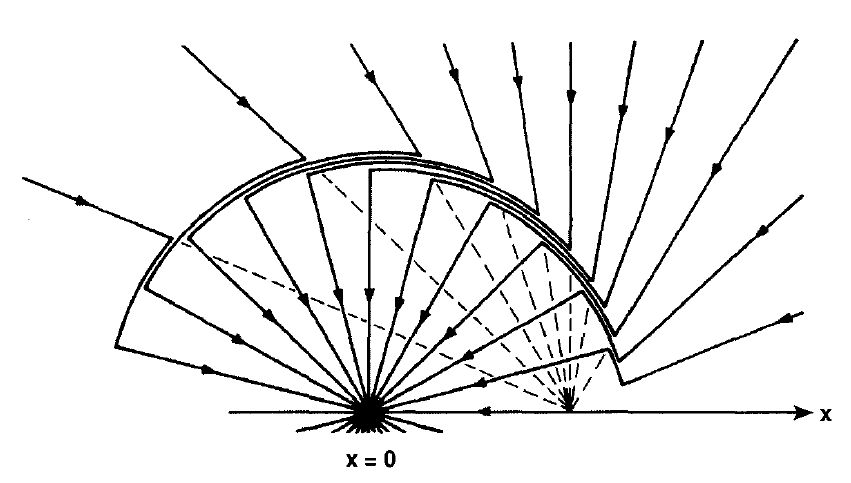
\includegraphics[width=0.8\textwidth]{\dir/figs/bremsstrahlung}
  \caption{The classical view of bremsstrahlung emission. Electric field lines are solid and dashed lines with arrows. The x-axis points to the direction of the particle movement. When the particle is abruptly stopped at x=0, two intense transverse electric fields are produced, generating an electromagnetic radiation i.e. bremsstrahlung. Adapted from \citet{haug2004elementary,asg1966berkeley}.}
  \label{bremsstrahlung}
\end{figure}

\paragraph{Laboratory micro-CT system}
A conventional X-ray source generates X-ray radiation by firing electrons onto a metal target in vacuum. The electrons were generated by thermionic emission from a heated metallic filament. The metallic filament and target are usually tungsten \citep{wildenschild2013x}. During the electrons impacting on tungsten, about 60\% of the energy is converted into heat, 39\% of the energy is lost due to backscatter, only 1\% of the input energy is converted into bremsstrahlung \citep{behling2015modern}.

There are commercial turn-key micro-CT system manufactured by a number of vendors. The turn-key micro-CT instruments have a wide range of specimen size, usually mm scale, and resolution from 100s of $\mu m$ to few $nm$. A summary of the available instruments on market can be found in the review by \citep{stock2008recent}. 

A conventional X-ray source generates cone-shaped X-ray beams, targeting a sample that mounted on a rotary stage. The X-rays are absorbed and diffracted, only part of the X-rays are able to penetrate the sample. The penetrated X-rays are captured by a detecting sensor and converted into signals (Fig.\ref{conventional}.

\begin{figure}[htbp]
  \centering
  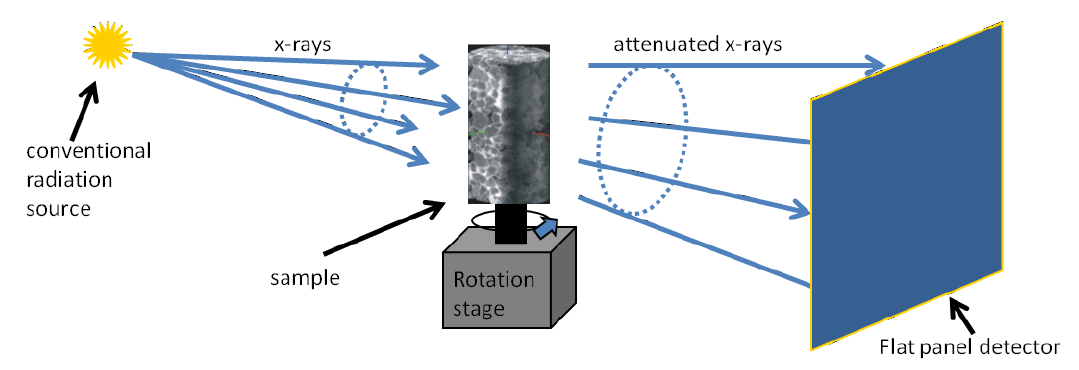
\includegraphics[width=0.8\textwidth]{\dir/figs/conventional}
  \caption{Cone beam configuration for conventional X-ray CT imaging. Cone-shaped X-ray beam is generated by an conventional X-ray source. The cone beam X-ray penetrates the sample mounted on a rotary stage and received by a detector. Adapt from \citet{wildenschild2013x}.}
  \label{conventional}
\end{figure}

\subsubsection{X-ray generated by synchrotron radiation}
Generally speaking, bremsstrahlung includes any radiation produced by decelerating a charged particle. Specifically, synchrotron radiation is a physical process of emitting radiation when charged particles being deflected in magnetic fields \citep{sokolov1966synchrotron}. Natural synchrotron radiation is called cosmic magnetobremsstrahlung \citep{ginzburg1965cosmic}. Man-made synchrotron radiation was first time observed in 1947 in the General Electric Research Laboratory in New York \citep{robinson2001history}. Synchrotron radiation can produce a wide range of  electromagnetic spectrum from infrared to X-rays. The upper limit of energy depends on the electron energy \citep{bonse1996x}. The X-ray generated by synchrotron radiation has very high emitted flux, thus the temporal resolution of synchrotron X-ray CT can be much finer than conventional X-ray CT.

\paragraph{Synchrotron light source and beam-line}
The first generation of synchrotron light sources were associated with high-energy particle colliders which primarily for particle physics studies. More recently, synchrotron light sources were built specifically for generating synchrotron radiation. 

Modern synchrotron light sources employs electron storage rings to accelerate and circulate electrons. An electron storage ring can reach a kilometre of circumference. Electrons and positrons (the counterpart of the electron) are accelerated to near the speed of light. The energy of the high-speed electrons are around 6-8 GeV, such high energy can generate extremely bright radiation that well above 10 KeV \citep{winicksynchrotron1987}. Magnetic fields are installed in the ring to steer and focus the accelerated particles. The high-speed electrons produce synchrotron radiation when they are deflected by the magnetic fields. The radiation spectrum spans widely from radio wave to visible lights, and to X-rays. The synchrotron X-ray radiation has very high photon flux and brilliance. High flux means large number of photons passing through an area in unit time, therefore imaging can be done fast, i.e. high temporal resolution. High brilliance means high intensity and directionality of the X-ray beam, therefore the X-ray beam can be focused on a small area, i.e. high spatial resolution\citep{wildenschild2013x}. Synchrotron X-ray is millions times brighter than conventional laboratory X-ray beams. The synchrotron radiation is projected tangential to the ring, and directed into each experimental station, often referred to as beam-lines (Fig.\ref{estoragering}.

beam-line consists of three major components. The synchrotron radiation exits the storage ring and enters the first component of the beam-line, the front-end. Then the radiation is filtered in the second component, the beam-line optics. The optimised synchrotron X-ray is then directed into the user's end, the experimental station \citep{wildenschild2013x}. Different beam-lines are built depending on the requirements of the study topics and imaging purposes. For example in the Advanced Photon Source in the Argonne National Laboratory (US), disciplines cover material science, biology and life science, geosciences and soil sciences, environmental science, chemistry, physics and polymer science.

\begin{figure}[htbp]
  \centering
  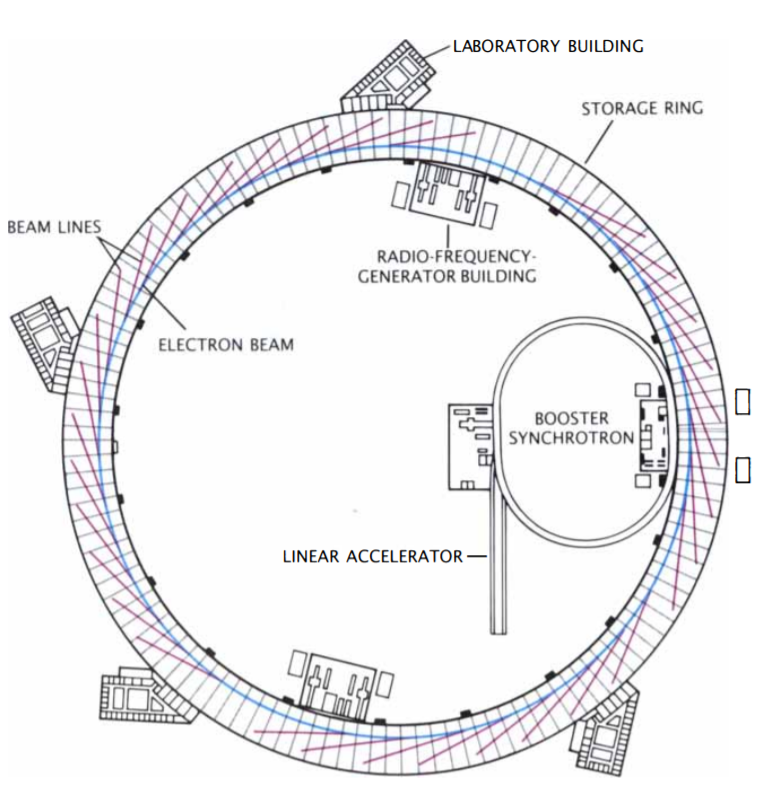
\includegraphics[width=1\textwidth]{\dir/figs/estoragering}
  \caption{A classical electron storage ring. Electrons are accelerated and stored in the ring (blue circle). Synchrotron radiation (purple lines) is produced when electrons are deflected by magnetic fields. Synchrotron radiations are guided into experimental stations that built tangential to the ring circumference. Image adapt from \citet{winicksynchrotron1987}.}
  \label{estoragering}
\end{figure}

X-ray beams generated by synchrotron radiation are parallel.  Fig.\ref{synchrotron} shows a typical synchrotron X-ray CT imaging configuration. X-ray beams pass through a monochromator, which select a narrow band of wavelengths of light, and through the target object. Penetrated X-rays are interacting with a scintillator screen that converts the X-rays to visible light, and finally reach the sensor device that converts the light into computer signals \citep{wildenschild2013x}.

\begin{figure}[htbp]
  \centering
  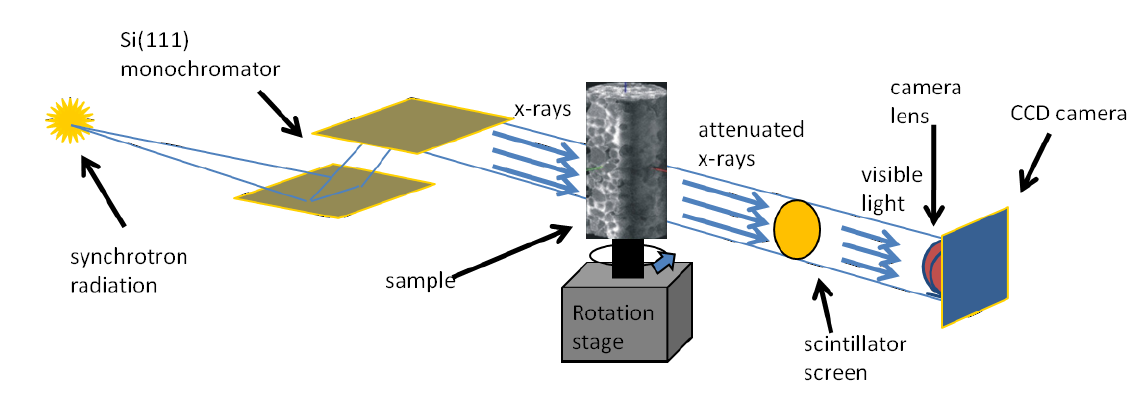
\includegraphics[width=0.8\textwidth]{\dir/figs/synchrotron}
  \caption{X-ray CT configuration of a synchrotron X-ray source. The X-ray beam from a synchrotron X-ray source is parrallel beam. The X-ray is filtered with a monochromator to obtain beam with constant energy and wavelength. The X-rays penetrates the target object on a rotary stage, and again filtered by a scintillator screen and converted to visible light. The visible light is captured by a camera. Adapt from \citet{wildenschild2013x}.}
  \label{synchrotron}
\end{figure}



\subsection{X-ray interactions with matter}
When X-ray photons interact with matter, they are absorbed, scattered, diffracted, refracted or transmitted through the material. When an X-ray photon is absorbed by an atom of the matter, electrons of the inner shell of the atom is ejected. The atom is ionised and neutralised, and emits an X-ray characteristic of the atom \citep{wildenschild2013x}. During this process of X-ray passing through the object, the X-ray intensity is attenuated. For an X-ray beam with constant energy and wavelength (i.e. monochromatic beam), this attenuation of X-ray follows the Beer-Lambert's Law:

\begin{equation}
    I=I_0exp(-\mu x)
\end{equation}

where $I_0$ is the incident X-ray intensity before passing through the object, $I$ is the attenuated X-ray intensity after passing. $x$ is the thickness of the object. $\mu$ is the linear attenuation coefficient that measures the easiness of X-ray passing through an object, higher $\mu$ means the X-ray is more attenuated after passing through an object. X-ray attenuation is majorly controlled by physical properties of the target materials and the X-ray interaction with the material. 

There are three fundamental interactions of X-ray with matter: the photoelectric effect, Compton scattering and coherent scattering (Rayleigh scattering) \citep{hsieh2003computed}. Only the first two types are important to the context of CT imaging, these two effects together decide the attenuation coefficient $\mu$:

\begin{equation}
    \mu= \tau + \sigma
\end{equation}

where $\tau$ is the photoelectric attenuation coefficient, and $\sigma$ is the Compton scattering attenuation coefficient.

\paragraph{Photoelectric effect}
The photoelectric effect was first explicated by Albert Einstein in 1905 and awarded the Nobel Prize in Physics in 1921. Fig.\ref{photoelectricandcompton} (a) illustrate a schematic process of the photoelectric effect during X-ray photon interacting with an atom. If the X-ray photon energy is greater than the binding energy of an electron of the atom, the photon contributes its entire energy to free the binding electron from an inner shell of the atom and then become vanished. The liberated electron is called a photoelectron. The inner shell is left with a vacancy for electron and thus replaced by an electron from the outer shell. This replacement of lower energy electron by higher energy electron will emit a characteristic radiation \citep{hsieh2003computed}. At low X-ray energy of 50-100 KeV, the interaction mechanism is dominated by the photoelectric effect and the attenuation coefficient $\tau$ is proportional to a power of the mean atomic number of the specimen \citep{wildenschild2013x}.

\begin{figure}[htbp]
  \centering
  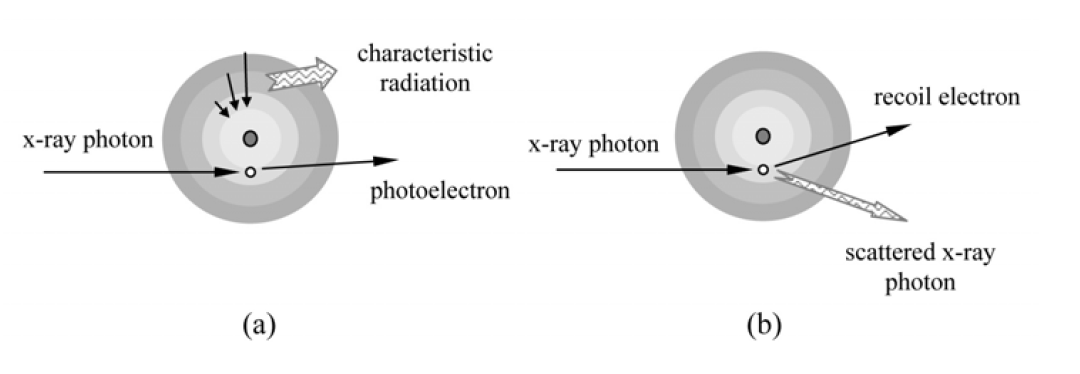
\includegraphics[width=0.8\textwidth]{\dir/figs/photoelectronandcompton}
  \caption{Photoelectric effect and Compton scattering. (a) shows the process of photoelectric effect, an X-ray photon interacts with an atom, produces a photon of characteristic radiation, a photoelectron and left a positive ion. (b) shows the process of Compton scattering, X-ray interacts with an atom, produces a scattered X-ray photon, a recoiled electron, and left a positive ion. Image adapt from \citet{hsieh2003computed}.}
  \label{photoelectricandcompton}
\end{figure}

\paragraph{Compton scattering}
Compton scattering was also a Nobel Prize-awarded (1927) finding, named after Arthur H. Compton. Fig.\ref{photoelectricandcompton} (a) illustrate a schematic process of the Compton scattering during X-ray photon interacting with an atom. This interaction is allowed to occur when the X-ray photon energy is much greater than the binding energy of an electron. The X-ray photon strikes an electron and cause it to flee from the atom. After the collision the incident X-ray photon is deflected or scattered and lost part of its initial energy. At high X-ray energy of 5-10 MeV the interaction process is via Compton scattering and the coefficient $\sigma$ is proportional to the electron density of the penetrated object \citep{wildenschild2013x, hsieh2003computed}. 

\subsection{CT image data}
\subsubsection{Grey scale images}
X-ray tomography records the intensities of X-ray attenuation of the target object, therefore X-ray μCT images are grey scale images that carry attenuation intensity information. An 8-bit grey scale image is composed of different shades of grey values ranging from black (intensity value = 0) as the weakest, to white (intensity value = 255) as the strongest intensity. In the following part of this thesis, the term intensity (if not specified else) is used to refer to grey values or brightness intensity rather than X-ray intensity. 

In the thesis, 16-bit and 8-bit images are analysed often, raw converted image from X-ray μCT are 16-bit (65536 levels) or 32-bit (4294967296 levels). Information is slightly lost during a conversion from higher bit depth to lower bit depth, but in return computational cost is reduced.

A binary image, or Boolean type data, has only two values - ones and zeros (also as Trues and Falses). Binary image is usually useful for extracting one particular feature from an image as foreground and the rest as background, for example porosity from a sandstone or pyroxenes from a gabbro. Binary images are also useful for isolating one label from multiple labels. For example isolating oil from fluids of water and oil.

\subsubsection{CT image resolution}
The spatial resolution of conventional CT is in the range of $mm$ scale. Computed X-ray micro-tomography (\textmu CT) expands CT resolution to $\mu m$-scale ($10^{-6}$ metre). The application synchrotron X-ray sources further extended the limit of spatial resolution of CT to below 1 \textmu m and enabled fast synchrotron-based X-ray \textmu CT, with scanning intervals reduced from hours to sub-seconds \citep{berg2013real}. 

High spatial resolution is crucial for higher imaging accuracy, the shape of the scanned object can be more accurately defined with higher spatial resolution, i.e. smaller pixel size (Fig.\ref{spacialres}).

\begin{figure}
    \centering
    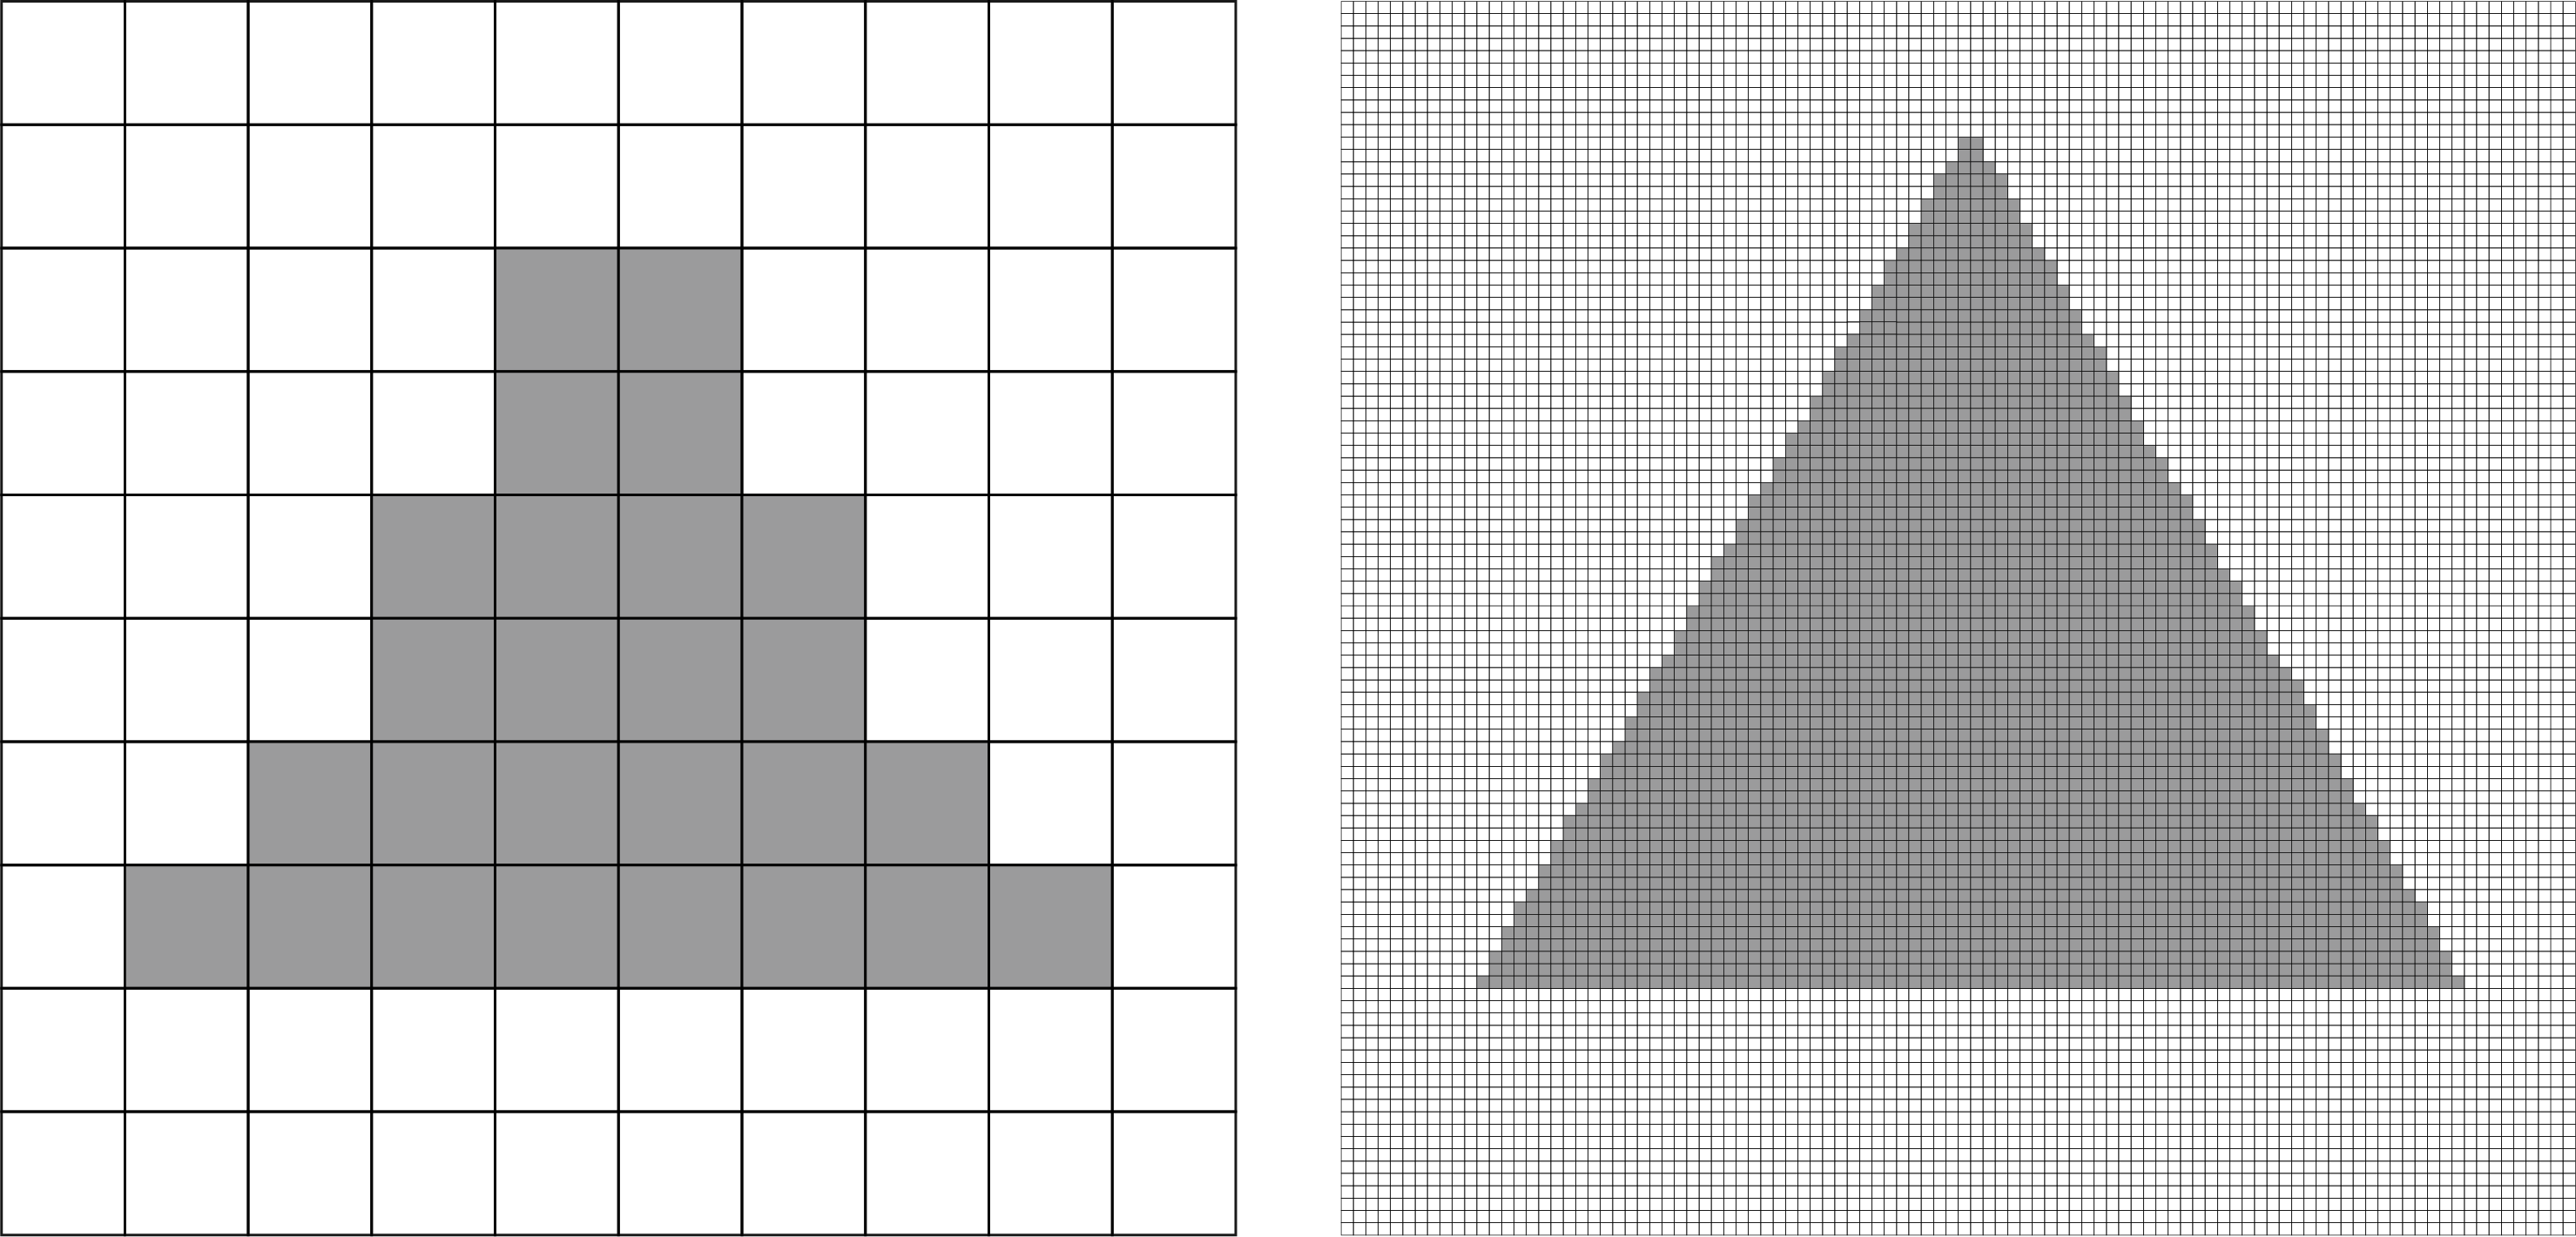
\includegraphics[width=1\textwidth]{\dir/figs/spatialresolution}
    \caption{Spatial resolution. Two triangles of same size were represented by low and high resolution. The level of proximity increase with resolution. \citep{CTscanartefacts}}
    \label{spacialres}
\end{figure}

\subsubsection{Pixel and voxel}
In digital imaging, a pixel is a value in a dot matrix data structure, and an image is a rectangular grid of pixels (Fig.
\ref{pnv} left figure). Pixels are square, and are the smallest element of a digital image. The length of pixels of a picture is defined by its resolution, higher resolution leads to smaller pixels. In X-ray μCT imaging, a pixel records the attenuation intensity of a finite point of the target object, and the intensity is represented by a grey scale value.
 
A voxel is a three-dimensional equivalent of pixel (Fig.\ref{pnv} right figure). Voxels represent values in three-dimensional space, and the position of a voxel is located by a three-dimensional Cartesian coordinate system. 

\begin{figure}
    \centering
    \includegraphics[width=1\textwidth]{\dir/figs/pixelnvoxel}
    \caption{Pixel and voxel. Left figure: pixels with different values in a 2D Cartesian coordinate. Right figure: voxels with different values in a 3D Cartesian coordinate \citep{CTscanartefacts}.}
    \label{pnv}
\end{figure}

\section{CT image processing part I: reconstruction and denoise}
\subsection{Overall workflow}
Image processing aims at identifying the objects presented in the image. A general CT image processing work flow is summarised in Fig.\ref{ctworkfl}. This work flow is abstracted from this study, the work flow may vary from different CT data sets as different imaging condition are applied and different demands for analysis required. In the following section the generic introduction of the CT image processing workflow is explained. The details of the specific work flow used in this study is further explained in the methodology chapter. In this chapter, the overall CT image processing workflow is introduced in two parts, the first part will start from image processing of data that directly acquired from CT instrument - projection images, to a more straight-forward representation of the imaged object - reconstruction images (the first row of blocks in Fig.\ref{ctworkfl}) . The second part will focus on extracting pragmatic information from the reconstruction images by segmentation, visualisation and measurements (the second row of blocks in Fig.\ref{ctworkfl}).

 \begin{figure}[htbp]
  \centering
  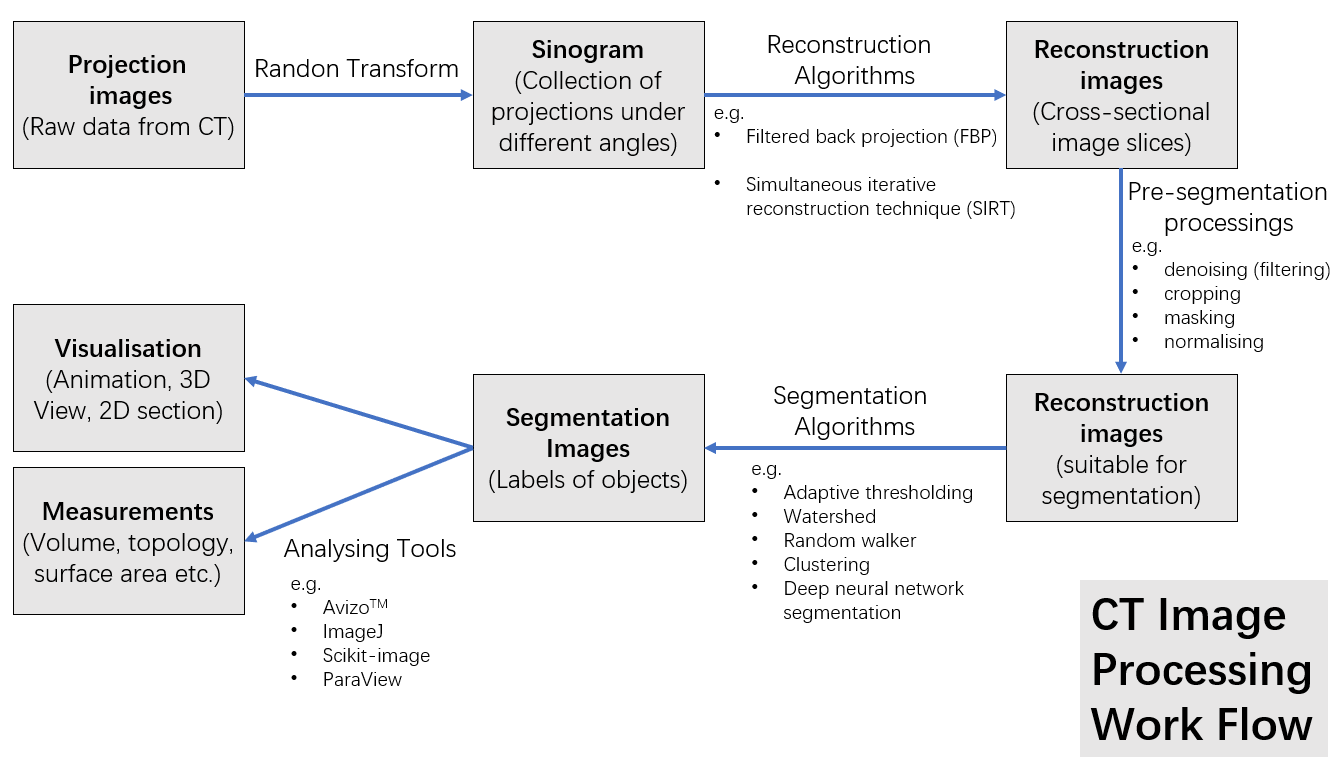
\includegraphics[width=1\textwidth]{\dir/figs/ctworkfl}
  \caption{A general summation of CT processing workflow used in this study. The projection images were converted into sinograms and Reconstructed images. The reconstructed images are segmented into labelled images that represent oil, brine and rock of the scanned object. Visualisation and measurements can then be carried out on the labelled segmentation images.}
  \label{ctworkfl}
\end{figure}

\subsection{Projection images} 
Raw data acquired from X-ray tomography are called projections images (or simply projections), they are X-ray projections of the target object from one particular angle. During an X-ray CT imaging process, the target object is imaged over a rotation of 360 degrees (for cone-beam instruments, but only 180 degrees for a parallel beam synchrotron set up), with step angle $\omega$ (Fig.\ref{ctrotangle}). The intensity of the penetrating X-rays are captured by a sensor device, and then processed into digital signals. These raw data acquired from X-ray tomography are called projections images, they are X-ray projections of the target object from one particular angle. The Projection images essentially carry information about the difference of X-ray absorption inside the object. Fig.\ref{psr} (A) shows one projection image (X-Y plane) from a micro CT scan of a cylinder carbonate rock sample.

\begin{figure}[htbp]
  \centering
  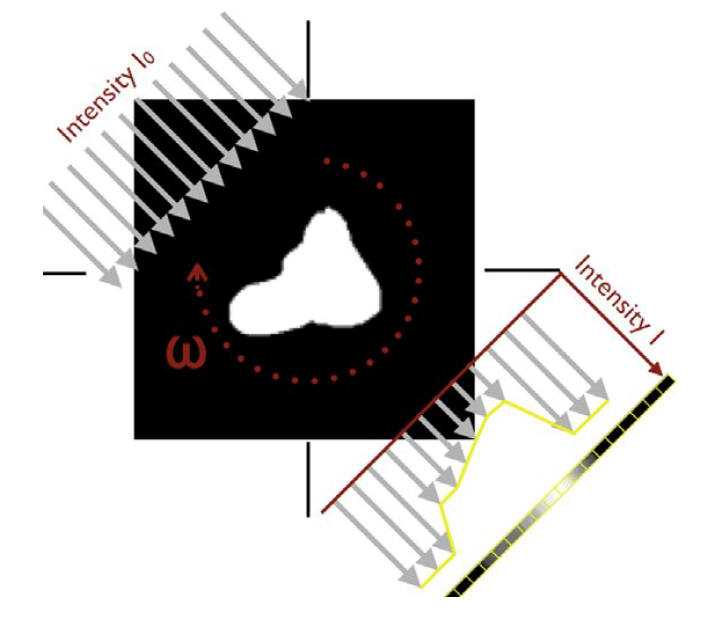
\includegraphics[width=0.8\textwidth]{\dir/figs/ctrotangle}
  \caption{Acquisition of CT projection. X-ray beam with initial intensity $I_0$ is attenuated by the object, the penetrating X-ray intensity $I$ is recorded as a line of pixels. This process is repeatedly carried out from $0-2\pi$ with rotation step$\omega$. Adapted from \citet{fusseis2014low}.}
  \label{ctrotangle}
\end{figure}

\subsection{Sinogram}
The collection of projections from different angles around the objects can be represented by sinograms that shows the absorption intensity signal at different rotation angles. This process is essentially the mathematical operation of Radon transform \citep{radon20051} of the projection image. 

\begin{figure}[htbp]
  \centering
  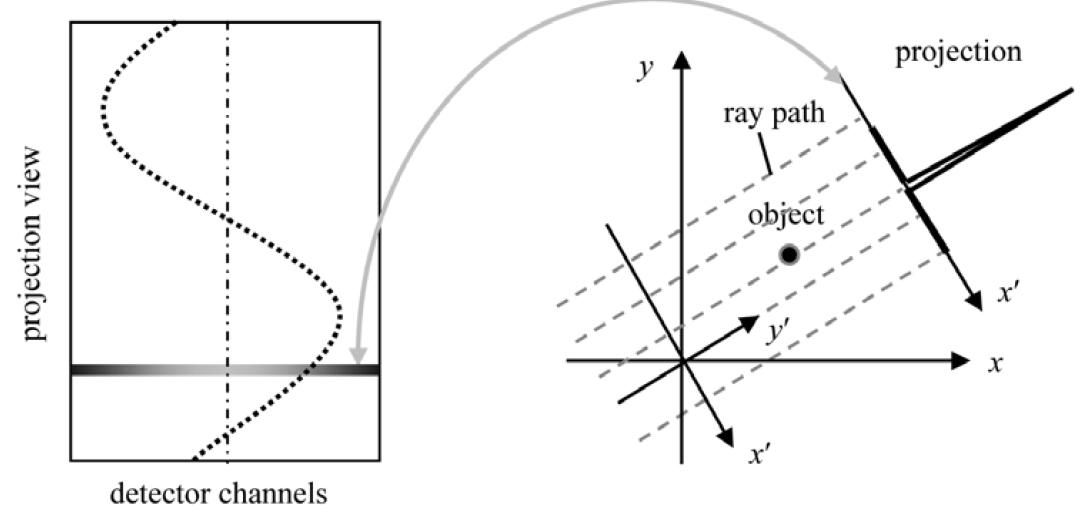
\includegraphics[width=0.8\textwidth]{\dir/figs/sinogram}
  \caption{Schematic diagram of the mapping between the sinogram space and the object space. A fixed point on the scanned object is represented as a sinusoidal curve. A single projection from a particular angle is represented as a horizontal line on the sinogram. Image adapted from \citep{hsieh2003computed}.}
  \label{sinogram}
\end{figure}

Fig.\ref{sinogram} shows schematic diagram of the mapping between the sinogram space and the object space. In the sinogram space, the X-axis represents the detection channels and the Y-axis represents the projection angle. There are two ways to interpret a sinogram. First, for a fixed point on the target object (shown as black dot on the right figure), its value of projection from different angles is recorded on the sinogram that forms a sinusoidal curve (left figure dotted curve). Another perspective to look into a sinogram is a line parallel with the X-axis, this line represent the intensity record of a single projection. Fig.\ref{psr} (B) shows the sinogram converted from the projection images. 

\begin{figure}[htbp]
  \centering
  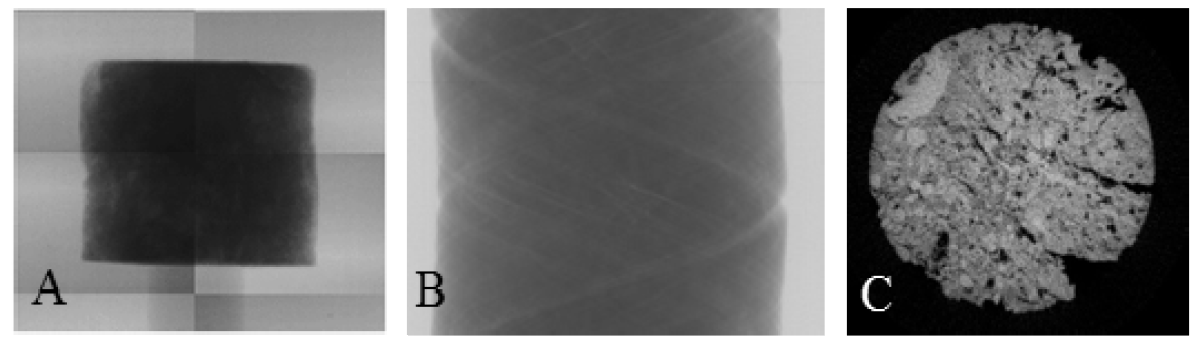
\includegraphics[width=0.8\textwidth]{\dir/figs/psr}
  \caption{Example of projection (A), sinogram (B) and reconstruction image (C) taken from a CT scan of a carbonate rock. \citep{Pak2014thesis}}
  \label{psr}
\end{figure}

\subsection{CT reconstruction}
Projections are a collection of X-ray measurements, of which each presents a summation of the attenuation coefficient of the object along a particular path of the X-ray beam. CT reconstruction is mathematically a inverse problem, of which the objective is to estimate the attenuation distribution of the imaged object using these measurements. By reconstruction, the projections are reconstructed into two-dimensional image slices (horizontal cross-sections) of the object (Fig.\ref{psr} (C)). CT image reconstruction is complicated due to various of factors and trade-offs such as the trade-off between spatial resolution and sample size, temporal resolution and noise, computational complexity and artefacts etc. Here only a brief overview of CT reconstruction relevant to this study is provided.

\subsubsection{Fourier transform and Fourier slice theorem}

Before introducing any reconstruction algorithm, first of all I will briefly introduce the Fourier transform, and the theory that governs tomographic reconstruction - the Fourier slice theorem \citep{kak2001principles} - in an intuitive explanation. 

Fourier transform is essentially a mathematical transform that decompose a signal function into constituent frequencies. It can present every non-linear function (e.g. an image, a song can all be seen as non-linear functions) by a sum of sine and cosine waves. For example, a photograph of a dog that human can recognise is in its spatial domain, where each pixel forms the shape of a dog. The photograph can be equivalently represented in the frequency domain that each point represents a particular frequency of the spacial domain image by performing Fourier transform.

The Fourier slice theorem states that: 

\begin{quote}
The Fourier transform of a parallel projection of an object $f(x, y)$ obtained at angle $\theta$ equals a line in a 2D Fourier transform off $f(x, y)$ taken at the same angle.
\end{quote}

In plain words, it implicates that, by performing 1D Fourier transform on each projection, we obtain a line in the 2D Fourier transform of the object. To fill the entire Fourier space of the object being reconstructed, we need a sufficient number of projections that surround the object from angle $0-\pi$. The complete Fourier space information can be used to recover the object by performing inverse Fourier transform.

\subsubsection{Filtered back-projection method}
The widely used reconstruction method is the filtered back-projection (FBP, \citet{herman1976convolution}), it has the balance of quality and efficiency therefore became the conventional method for reconstruction. The filtered back-projection method is based on the Fourier slice theorem (Fig.\ref{fbp}). In order to reconstruct the object using the theorem, we need to perform inverse Fourier transform on 2D Fourier transform of the object. The 2D Fourier transform is obtained by 'patching together' all 1D Fourier tranforms. For a cylindrical object, ideally we want the 1D Fourier transform of circular sector shape (Fig.\ref{fbp} (a)), because that would prevent any overlapping when 'patching together' all 1D Fourier transforms. Realistically, the 1D Fourier transform is rectangle shaped (Fig.\ref{fbp} (b)). Simply summing up the 1D Fourier transforms will cause overestimation in the centre of the cylinder but underestimation on the peripheral of the cylinder. To solve this problem, the rectangle shaped 1D Fourier transform is multiplied by a weighting function ((Fig.\ref{fbp} (c)) to approximate the ideal shape (a).

\begin{figure}[htbp]
  \centering
  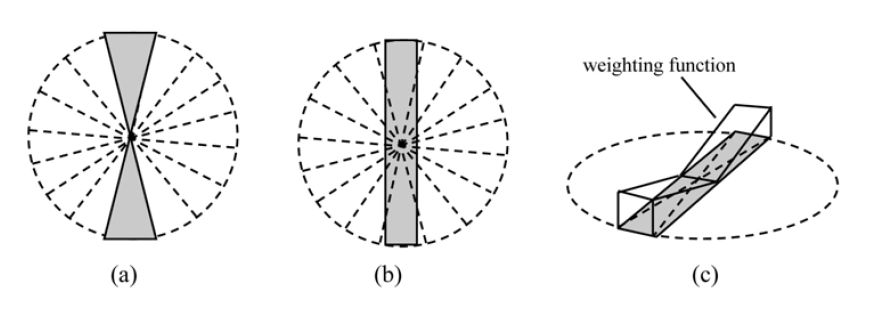
\includegraphics[width=0.8\textwidth]{\dir/figs/fbp}
  \caption{Conceptualised illustration of filtered back-projection method. (a) is idealised shape of area to use 1D Fourier transform. (b) is realistic shape of area to use 1D Fourier transform. (c) is realistic area optimised with a weighting function to approximate the ideal shape (a). Image adapted from \citet{hsieh2003computed}.}
  \label{fbp}
\end{figure}

\subsection{Artefacts in reconstructed CT images}
Artefacts are systematic discrepancies between the reconstructed image and the true image \citep{barrett2004artifacts}. In CT derived images, artefacts are essentially discrepancies between the reconstructed values in an image and the genuine attenuation coefficient of the object. Artefacts can occur as streaking, shading, rings and distortions etc., and to some extent degrade the quality of CT images. Artefacts are produced both at the CT data acquisition stage, by intrinsic physical processes and imperfections in the CT instrument, and at the data reconstruction stage. Artefacts can be avoided, corrected or alleviated by proper methods. All artefacts affect the absolute grey scale distribution of an image, and so must be avoided if good image classification is to be achieved.

\subsubsection{Physics-based artefacts}
Physics-based artefacts are generated from physical processes of CT scanning, such as the absorption of the X-ray beam. 

\paragraph{Beam Hardening}
The mean energy of a poly-chromatic X-ray beam increases (becomes "harder") as the beam penetrates an object due to faster absorption of the lower-energy photons; this is beam hardening. Beam hardening mainly produces cupping artefacts for cylindrical samples, where the  total brightness of the X-ray beam is reduced by adsorption of low energy photons in the middle of the cylinder than it in the peripheral of the cylinder. This leads to a characteristic cupped-shaped X-ray intensity profile along the cylinder. In very heterogeneous samples, beam hardening can also lead to streaks and dark bands. Beam hardening can be minimised by using filtration, calibration correction and beam hardening correction software, or avoided by using monochromatic beams at Synchrotron facilities \citep{barrett2004artifacts}.

\begin{figure}[htbp]
  \centering
  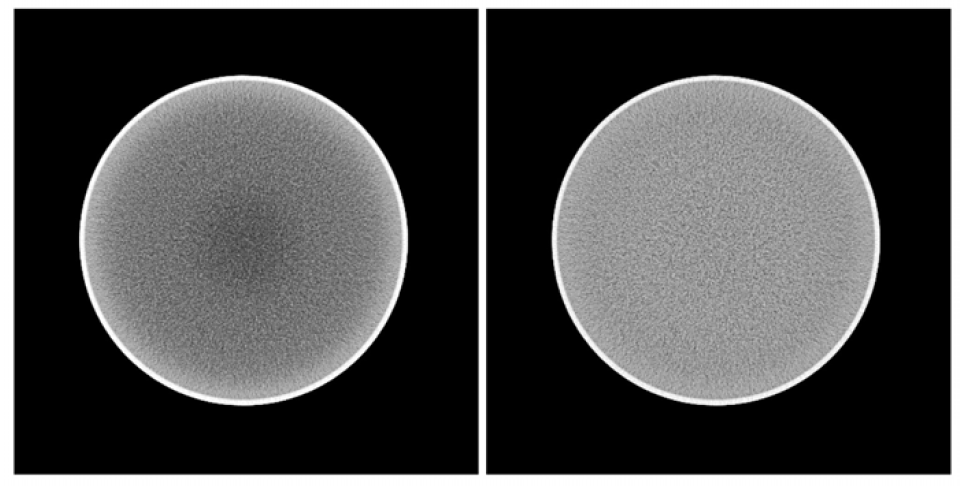
\includegraphics[width=0.8\textwidth]{\dir/figs/bh}
  \caption{ Reconstructed images of a 35-cm water phantom. Left figure shows cupping artefact caused by beam hardening. Right figure shows CT reconstruction image without beam hardening. Image adapted from \citep{hsieh2003computed}.}
  \label{bh}
\end{figure}

\paragraph{Partial Volume effect}
Partial volume effect (Fig.\ref{pve}) refers to the phenomenon that the grey scale value of a pixel/voxel is a representative of the average attenuation of the materials within a voxel \citep{barrett2004artifacts}. It is due to that inside the size of one voxel there exists more than one material with different attenuation coefficients. The effect can cause the appearance of artefacts such as shading and blurring. Increasing the spatial resolution of CT can alleviate this problem, i.e. containing more than one material within a voxel occurs less frequently when the size of the voxel is smaller. This effect can not be eliminated.

\begin{figure}
    \centering
    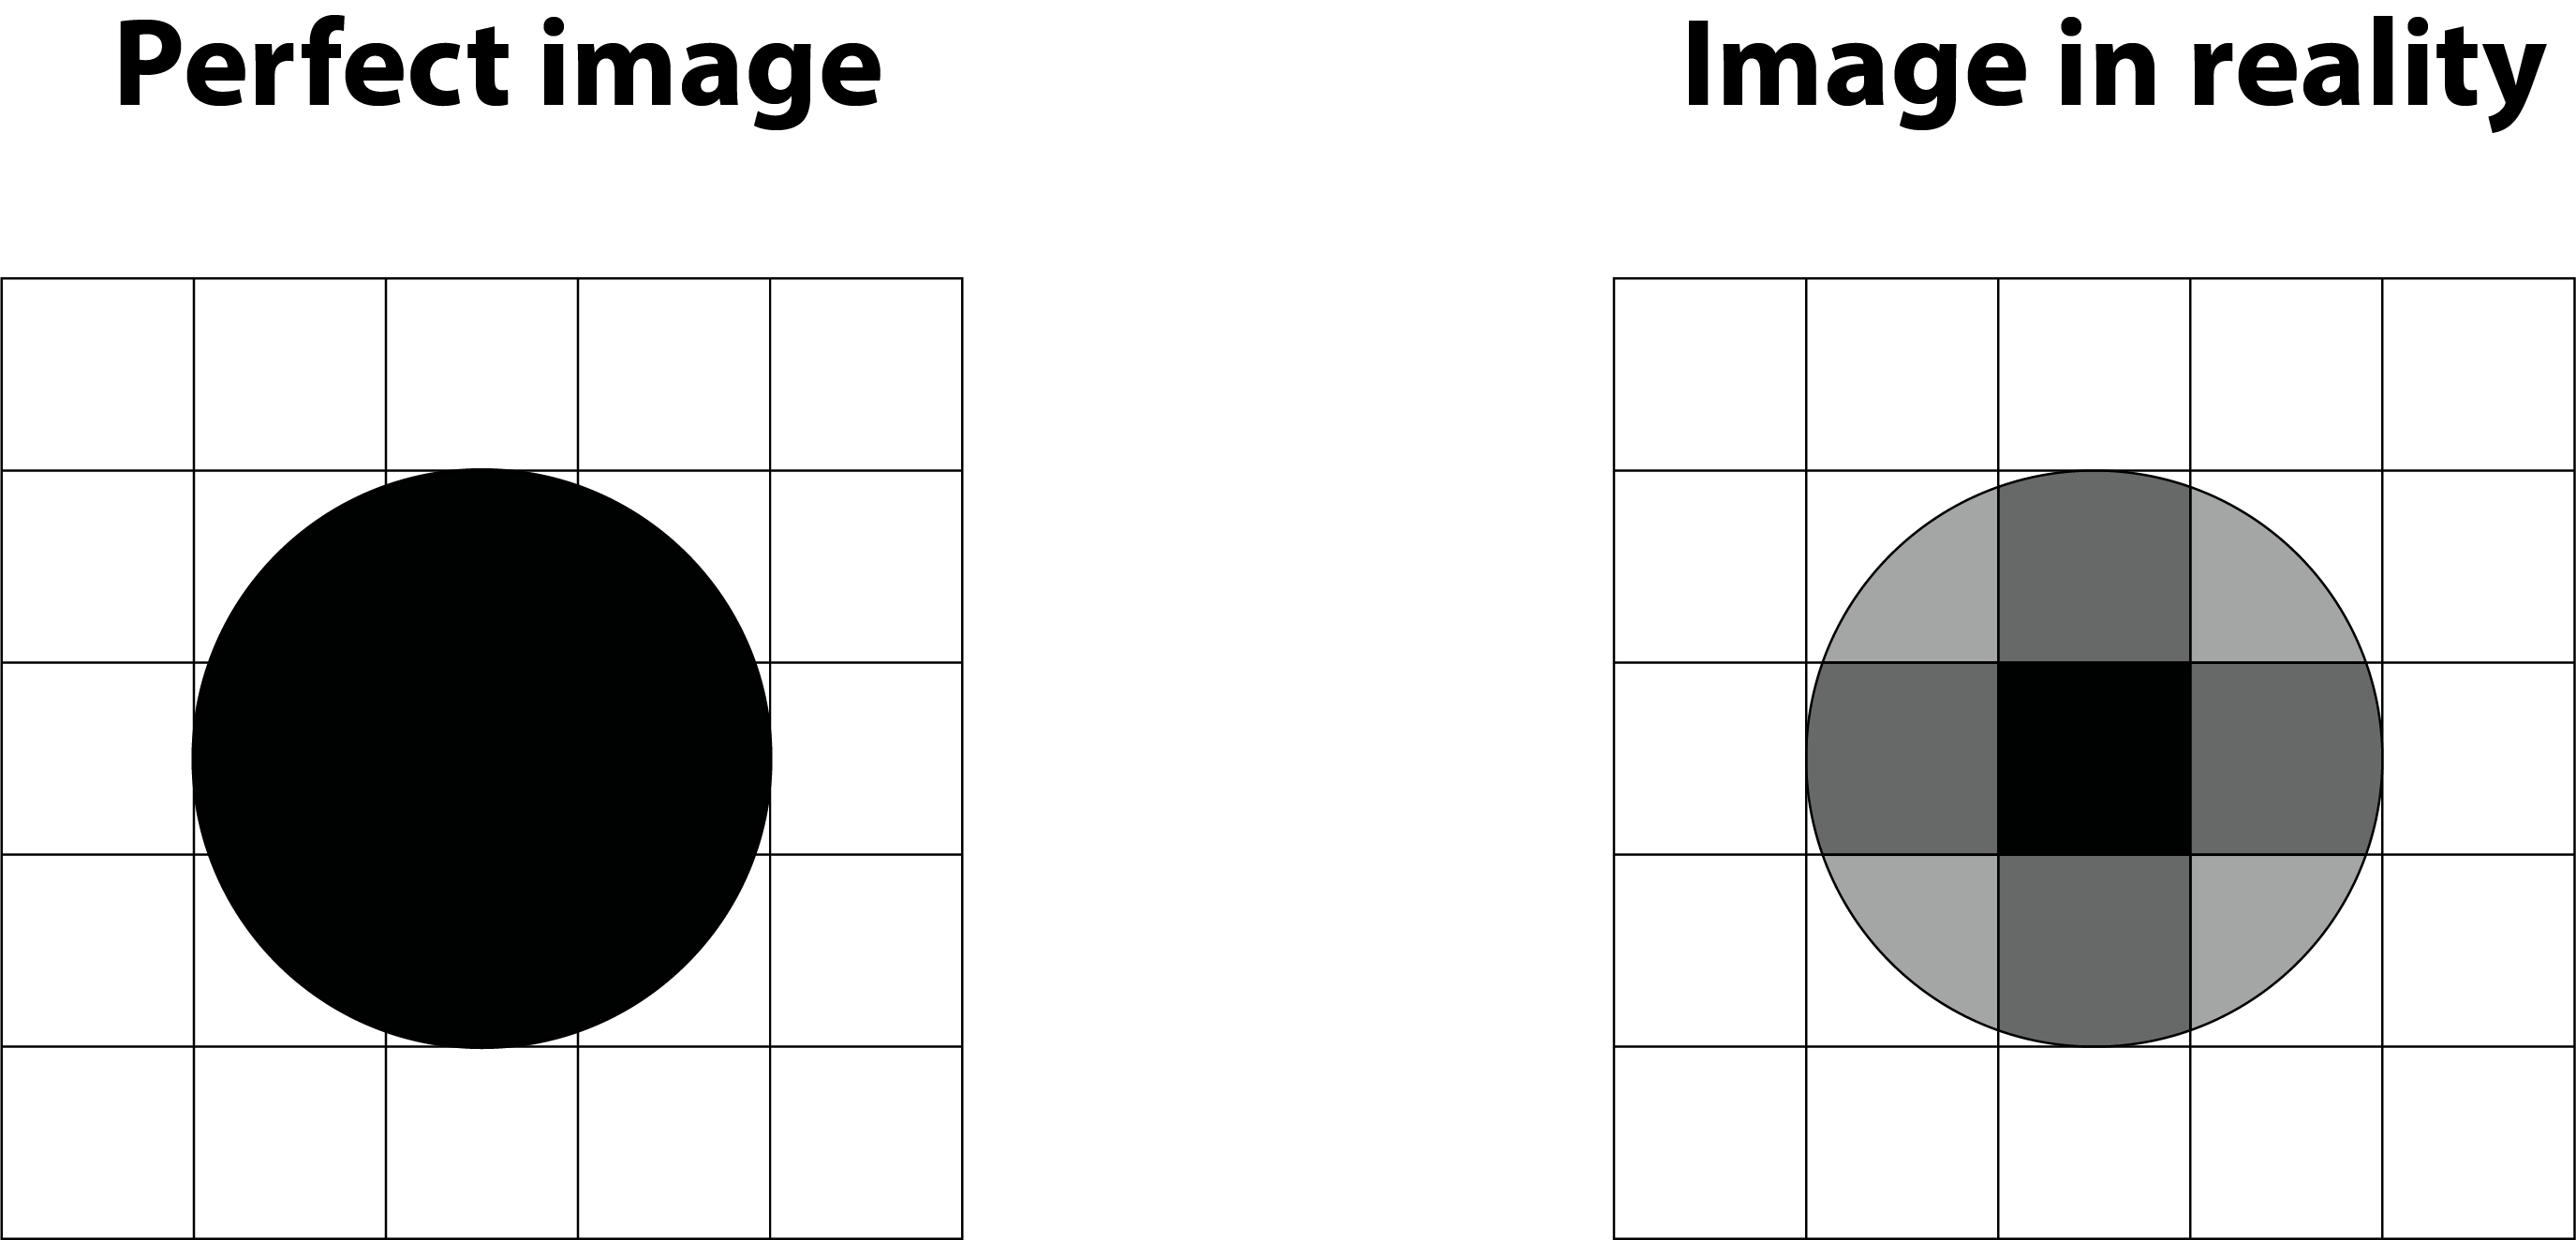
\includegraphics[width=1\textwidth]{\dir/figs/partialvolume}
    \caption{Partial volume effect of a solid circle. Left figure shows the perfect image without partial volume effect. Right figure shows realistic image that the pixels on the border of the circle containing two phases, therefore their intensity are averaged by the circle and the outside. Image adapted from \citep{CTscanartefacts}.}
    \label{pve}
\end{figure}

\paragraph{Under-sampling} 
Under-sampling happens when the angular intervals between projections are too large. It produces aliasing that appears as fine radiating stripes. Aliasing can be minimised by acquiring a larger number of projections per rotation \citep{barrett2004artifacts}. The fine, radiating stripes that at a distance from the object is called view aliasing, and the stripes that close to the object is called ray aliasing (Fig.\ref{undersamp}).

\begin{figure}
    \centering
    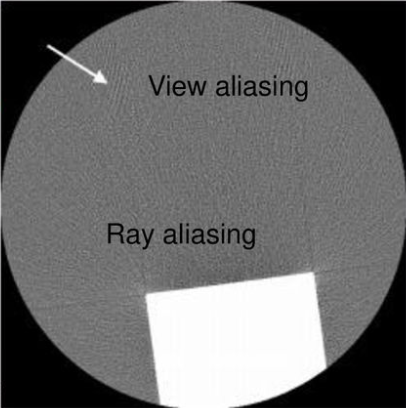
\includegraphics[width=0.6\textwidth]{\dir/figs/undersamp}
    \caption{View aliasing and ray aliasing of a cube phantom caused by undersampling. View aliasing occurs a distance away from the object. Ray aliasing occurs close to the object. Image adapted from \citep{CTartifacts}.}
    \label{undersamp}
\end{figure}

\paragraph{Photon Starvation} 
When the X-ray beam attenuation is too high, or the X-ray beam is too sparse thus photons recorded by the camera are insufficient, highly noisy projections are produced. This is called photon starvation. It usually leads to streaking artefacts \citep{barrett2004artifacts} (Fig.\ref{photonstarvation}). In most of the geo-scientific studies, photon starvation can be overcome by increasing the X-ray energy, as it is unnecessary to consider X-ray dose.

\begin{figure}
    \centering
    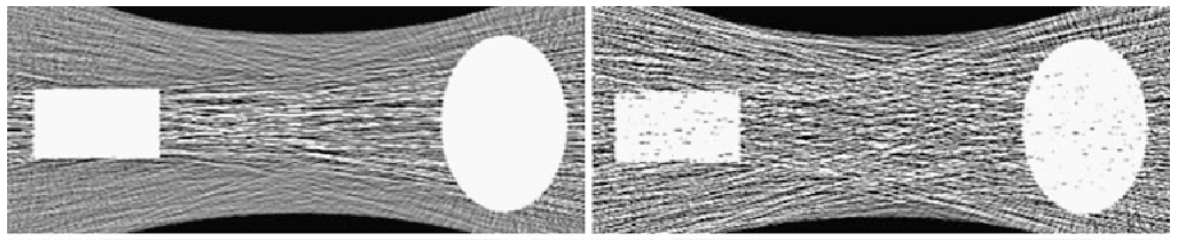
\includegraphics[width=1\textwidth]{\dir/figs/photonstarvation}
    \caption{Photon starvation artefact in a CT image of a rectangle phantom and a ellipsoid phantom. Left figure and right figure are scanned with X-ray beam of 225,000 and 40,000 photons per ray. The right CT image with less photons per ray appears more noisy. Image adapted from \citep{mori2013photon}.}
    \label{photonstarvation}
\end{figure}


\subsubsection{Hardware-based artefacts}
\paragraph{Ring artefacts} 
Ring artefacts are concentric circle artefacts. They are very common in CT scans and mostly due to non-linear behaviour of individual camera pixels, i.e. the output response to input from the camera scintillator is out of step with the neighbouring pixels. Radiation damage also can lead to bad pixels. Ring artefacts can be minimised by re-calibration, or using filter software.

\begin{figure}[htbp]
  \centering
  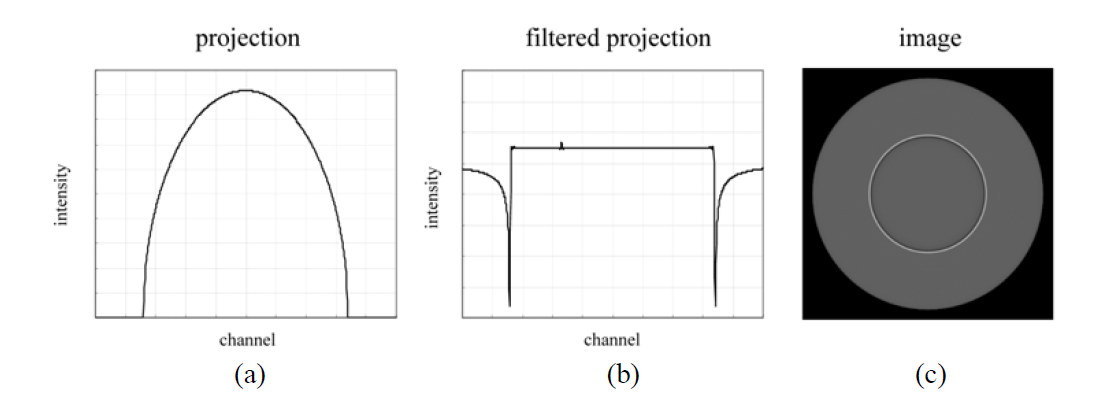
\includegraphics[width=1\textwidth]{\dir/figs/ring}
  \caption{Artificial ring artefact. About 1\% of error was added to a single channel over all projection angles. (a) Projection profile with 1\% added error. (b) Profile after filtering operation. (c) Reconstructed image with a bright ring artefact in the middle. Image adapted from \citet{hsieh2003computed}.}
  \label{fbp}
\end{figure}

\subsection{Noise in reconstructed CT images and denoising methods}
Noise is a random, variation of grey values in images. Unlike artefacts, noise does not inherent to the CT imaging process or the CT instrument, but inherent to the more generalised process of electric signal processing. Noise is produced in multiple ways, the generation of noise and denoising methods are extensively studied in data science and signal processing science.

\subsubsection{Source of noises}
There are four major sources of noise: random noise, statistical noise, electronic noise and round off mistakes \citep{diwakar2018review}.

\paragraph{Random noise} 
Random noise is generated by activities in the environment where X-ray CT scan is being carried out. Random noise is also referred to as 'white noise', because like the colour white that includes all the colours of a spectrum, white noise contains all frequency harmonics in approximately equal magnitude. 

\paragraph{Statistical noise}
During the transmitting of a finite number of X-ray photons, the number of photons detected by the camera device may vary between measurements because of statistical fluctuation. For pixels that receive photons via beam paths that have the same total attenuation, the number of photons recorded is not identical but is represented by a population. This is known as statistical noise, or quantum noise. That population gets narrower as the total number of photons detected increases. Statistical noise is reduced by increasing the number of detected photons.

\paragraph{Electronic noise}
The electronic circuits that detecting the analogue signal have inherent noise, like electromagnetic interference, thermal agitation or radio frequency interference. These noise can affect the process of receiving X-ray signals. This is the electronic noise. It is minimised by carefully engineered CT instrument.

\paragraph{Round-off errors}
All X-ray signals are ultimately processed by computer. So there is inevitable process of converting signals from binary system to decimal system. Due
to limited number of bits for storage of discrete signals in computer system, the mathematical computations have to involve round-off operations. The noise brought by round-off operations is round-off error\citep.

Reconstructed CT images may be affected by a mixture of noises from the above sources. But in general, the noise distribution in CT images can be characterised by Poisson distribution or Gaussian distribution \citep{diwakar2018review}.

\subsubsection{Denoising methods}
CT derived images generally have some degree of noise. It is assumed that an image with noise is the summation of the desired image and a noise component \citep{diwakar2018review}. Noise affects the quality of the CT image therefore can cause problems during analysis of the image data. Denoising is the task of reducing the noise component as much as possible, while preserving the original image pattern to recover the desired image. In this section some frequently used denoising methods are introduced, for further knowledge \citet{diwakar2018review} provid an extensive and detailed review on denoising methods.

\paragraph{Median Filter} Random noise in CT images can be reduced by using denoising algorithms as known as filters. The most common type of filters are local smoothing filters (also known as neighbourhood filters). This kind of filters restores a pixel by taking average of its neighbouring values. Taking a $3\times3$ median filter \citep{huang1979fast} as example (Fig.\ref{median}), a window size of $3\times3$ pixel is sliding across the image, and the value of the central pixel is replaced by the median of the greyscale values of the 9 values. One benefit of using the median rather than mean (known as mean filter) is that outlier values can significantly affect the mean value but not the median value. This algorithm can significantly reduce the outlier noise and therefore 'smooth' the noisy image. Though simple and fast, the median filter smooths the entire image regardless of the boundary pattern of objects. 

\begin{figure}[htbp]
  \centering
  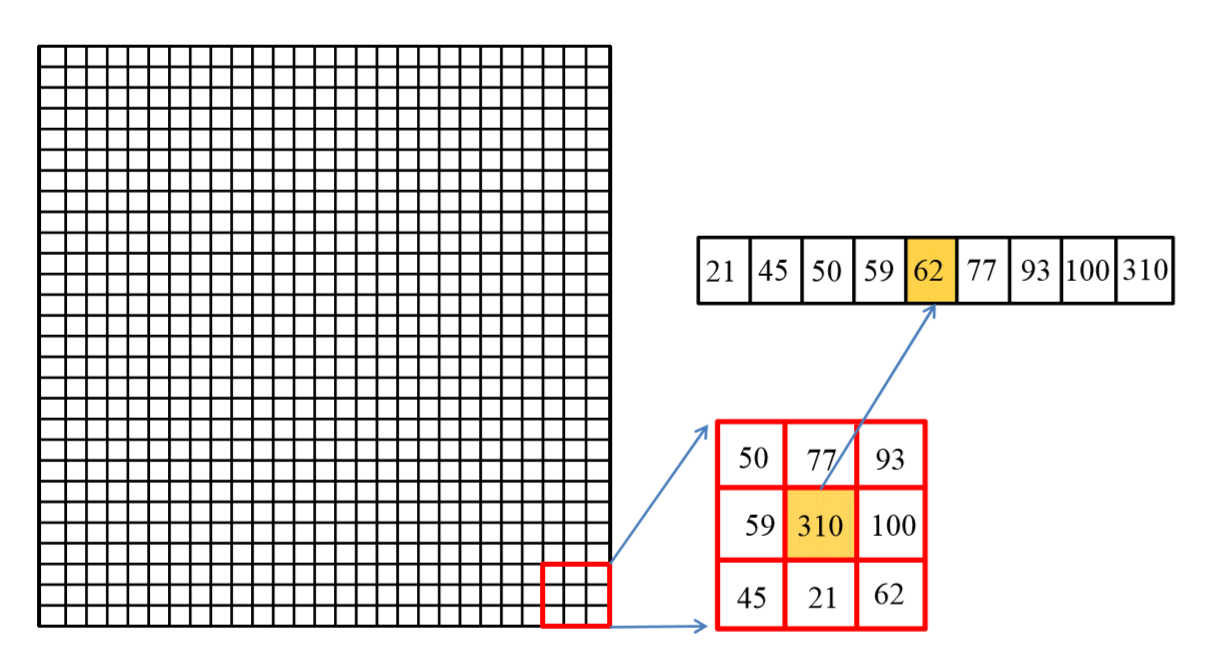
\includegraphics[width=1\textwidth]{\dir/figs/median_filter.png}
  \caption{Application of a 3x3 median filter on a 2D image. The red matrix shows the kernel and its neighbourhood window. The median number 62 was taken as the filtered value of the kernel. Image from \citet{Pak2014thesis}.}
  \label{median}
\end{figure}

\paragraph{Bilateral filter}
Median and mean filters have the major problem of obscuring the boundaries and small features of image patterns. \citet{tomasi1998bilateral} introduced the bilateral filter which removes noise while preserving the boundaries. The bilateral filter takes the geometric closeness and photometric similarity of the pixels inside/outside the window into account, and replaces the pixel value with an average of similar and nearby values.

The bilateral filter defines similarity functions that measures both the geometric closeness and photometric similarity. In 'smooth' regions i.e. inside a image pattern that does not include boundaries, the bilateral filter acts the same as the mean filter. When a sharp boundary presents in the window, the similarity functions splits the window into two sides defined by the boundary. As a consequence, the smoothing only affects either side and the boundary is preserved.

However, \citet{buades2011non} questioned the approach with the idea that '\textit{the most similar pixels to a given pixel have no reason to be close at all}'. He introduced a similar but more advanced and increasingly used filter called the 'non-local means' filter \citep{buades2011non}. The non-local means filter is adopted in this study and is introduced in chapter three.

\paragraph{Other methods}
In this study various of denoising filters were tested on the data, in this section I will briefly introduce the methods that have been tested. The methods introduced above belong to the category of spatial domain filtering, i.e. by applying filters directly on original noisy image. In this category, there are other denoising algorithms which practise the least square fidelity minimisation concept \citep{yan2011new, yan2011power,yan2012smoothed}. To name a few Tikohonov \citep{tikhonov1978methods}, anisotropic diffusion \citep{perona1990scale}, total variation \citep{chambolle2004algorithm} methods and the combined anisotropic total variation \citep{rudin1992nonlinear} method. Another category parallel with the spatial domain filtering is the transform domain filtering. Rather than directly filter the original noisy image, the noisy image is decomposed into different frequency components called wavelets (i.e. wavelet transform \citep{mallat1989theory}). The widely studied domain in this category is the non-linear coefficient thresholding based methods \citep{mallat1989theory}. With the state-of-art deep learning algorithms being powerful in solving image-related problems, convotional neural network (CNN) denoising approaches are increasingly investigated (e.g.\citep{kang2017deep,chen2017low,chen2017low2,gondara2016medical}).


\section{CT image processing part II: Segmentation}
To analyse and quantify X-ray μCT derived geological images, different constituents, for example intensities or textures, on the image needs to be classified into non-overlapping regions that represent oil water and solid. This process is called segmentation, it is the major processes in analysing and extracting quantitative information relating to the properties of the digital images. The quality of segmentation critically affects the downstream analysis of the scientific process.

However, there are some factors that influence the quality of the images, thus cause difficulties in segmentation. First, natural geological samples are usually highly heterogeneous in both mineralogy and geometry, this leads to usually sub-resolution features that cannot be identified. Second, CT images are affected by partial volume averaging, where the greyscale value of a voxel is the average of the values within a voxel, thus distorts the image \citep{barrett2004artifacts}. Third, instruments caused artefacts and noises. These problems can be wholly or partially alleviated by a pre-processing step before segmentation. Additionally, the data produced by X-ray μCT are essentially recordings of attenuation values that are uncalibrated with respect to actual composition, and the information is interpreted by human observation with other supporting observations such as Electron Microprobe Analysis (EMPA) and Scanning Electron Microscope (SEM). This means that discrepancy in different interpretations will also affect the segmentation. 

In practice, one or a combination of segmentation algorithms is used to assign every pixel with a label, so pixels with the same label are in the same category. Categories are usually defined according to the interpretation of the image, such as different mineral phases or different parts of a fossil. The outcome of image segmentation is a map of labelled areas that shows the spatial distribution of different objects. 

\subsubsection{Segmentation methods}
By Khan’s (2013) classification, image segmentation methods can be classified into six major categories. They are: 1) Threshold based; 2) Region Based; 3) Edge based 4) Fuzzy Theory based 5) Artificial Neural Network (ANN) based and 6) Partial Differential Equations (PDE) based. A segmentation algorithm is a set of computer operations that execute the segmentation methods. This section introduces major segmentation algorithms tested and related with the work described in this. 

\paragraph{Thresholding}
CT images consist of pixels that record the X-ray attenuation which reflecting the density and mean atomic number of the object and the energy of the incident X-rays. Therefore the main difference between different materials is the intensity value of the pixel. Thresholding is the most straight-forward, intensity-based segmentation method. By choosing an intensity threshold, the intensity values above and below the threshold are separated into two domains. Either domain represents one of the materials to be segmented. 

For the ideal case, where the intensity values of two different materials do not overlap at all, thresholding is easy and straight-forward. However for most real cases, two intensity distributions almost always overlap to some extent due to artefacts, noises and potentially compositional variations. Therefore, segmentation by thresholding often mis-classify the overlapped intensity (Fig.\ref{thresholding}). Nonetheless, for CT images with good contrast and low noise, thresholding is generally a good choice.

\begin{figure}[htbp]
  \centering
  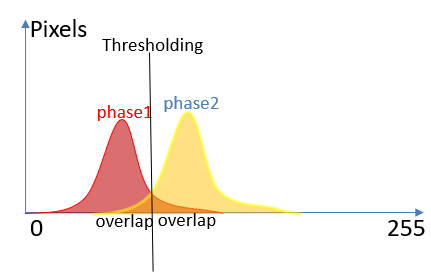
\includegraphics[width=1\textwidth]{\dir/figs/thresholding.png}
  \caption{Schematic illustration of thresholding an 8-bit image. Two phases on the image have different but partly overlapped distribution of intensity (red and yellow). By defining a threshold value the two phases are roughly separated, however thresholding can not handle the overlapping part of the intensity distribution. Therefore these pixels with overlapping intensity are mis-classified.}
  \label{thresholding}
\end{figure}

The optimal thresholding value can be chosen by trail and error. There are also automated algorithms for thresholding, the mostly used ones are Otsu method \citep{otsu1979threshold} for 2-phase thresholding and K-means clustering \citep{ridler1978picture} for multi-phase thresholding. 

In some CT images, the same material can have varied contrast due to intensity fluctuation by artefacts and noises. The variation can occur across different CT batches, or across different image slices, and even different regions within a single image. In this case there exists no single 'global' thresholding value that can be applied to all regions/images. This problem can be solved by adaptive thresholding (e.g. \citet{sauvola2000adaptive},\citet{niblack1986introduction})that uses local information to calculate the thresholding values for different regions. 

In conclusion, thresholding is the simplest of the common segmentation methods, however it has the shortcoming of low tolerance to noise and artefacts. The direct use of thresholding on CT images often leads to vast mis-classification. For CT images with less ideal quality, more advanced segmentation methods are proposed.

\paragraph{Watershed}
Watershed is one of the mostly used segmentation algorithms in CT image processing. It is a region-based segmentation method originated on the theory of mathematical morphology \citep{serra1986introduction}.

In a CT image, there are pixels with high and low intensity values distributed as patterns. In watershed segmentation, the image is regarded as a topographic landscape, where the maxima of intensity values represent "ridges" and the minima of low values are "valleys". The elevations of this landscape are defined by grey values or the gradient magnitudes of individual pixels. With this idea, the image is decomposed into numbers of non-overlapping \textit{catchment basins} separated by \textit{watersheds}. Then the \textit{catchment basins} are mathematically "flooded" such that some regions on the image begin to merge. The merging is supported by a method called \textit{merge tree} to characterise the best level of merging. The image is segmented when the best level of merging is achieved.

Marker-based watershed method allows users to explicitly define specific positions, usually local maxima/minima, to produce better segmentation. 

\paragraph{Random walker}
Random walk is a mathematical problem raised by K. Pearson in 1905. The random walker is a segmentation algorithm based on solving the Dirichlet problem, adapted to image segmentation by \citet{grady2006random}. It uses pre-labelled pixels as markers, and judges segmentation by the highest probability that unlabelled pixels reach pre-labelled pixels by random walks. The random walker is formulated in discrete space thus allowing it to be performed in arbitrary dimensions. This algorithm is extensively used in this study and will be introduced in detail in the methodology chapter (Chapter three).

\paragraph{Deep learning segmentation}
The state-of-art deep learning algorithms, especially the convolutional neural network (CNN), have been proved effective in image-related tasks in a revolutionary way. It is essentially a segmentation method by training a model classifier using a vast number of labelled data. In this thesis I implemented the convolutional neural network on CT image segmentation and increased the segmentation efficiency from hours to minutes for a single CT volume comparing with conventional segmentation routine. The detail of this method is described in Chapter four.

\subsection{Measurements of CT derived geological images}
The segmented CT images are ready for quantification and scientific analysis. There are numbers of measurements that are useful in geological CT image analysis.

\paragraph{Representative elementary volume}
Representative Elementary Volume (REV) is the smallest unit volume over which measurements can represent the whole sample. Sample REV has to be at least no larger than the targeted volume to show a representative result. 

\paragraph{Volume}
The volume of the void space in segmented images can be directly measured as the porosity, the measurement is always smaller than the genuine porosity due to the exclusion of sub-resolution micro-porosity that can not be clearly imaged. Volume of fluids can be directly measured, and therefore the fluid saturation can be derived as the ratio of fluid volume to porosity.

\paragraph{Pore network characteristics}
Pore network characteristics can be directly measured from the segmented images, or indirectly measured by pore network modelling methods. The characteristics includes porosity, absolute and relative permeability, pore aspect ratio (the ratio of longer axis to shorter axis of a pore), pore size distribution, surface area and connectivity of the pore network.

\paragraph{Curvature}
Curvature measurement is important for fluid flow in porous medium, as it is the important property from which can be derived the capillary pressure. Curvature for a point on a 2D curve is simply the inverse of its inscribed radius. Curvature for a point on a 3D surface has two independent principal curvatures. Curvatures are difficult to measure and are extremely sensitive to noise and artefacts \citep{wildenschild2013x}. \citet{armstrong2012linking} measured oil-water interfacial curvature in drainage-imbibition cycles. They estimated capillary pressure via the Young-Laplace equation and the estimation shows good agreement with experimental measurements from a pressure transducer. \citep{andrew2015imaging} measured $CO_2$-brine interfacial curvature in drainage events and their relation to snap-off events of both local and distance. They visually confirmed the presence of terminal meniscus and arc meniscus as two types of interface in a porous medium.

\paragraph{Contact angle}
Contact angle is an extremely important measurement in the field of fluid flow in porous media as it essentially characterise the wettability. However the measurement of contact angle is difficult due to the heterogeneity of the wettability in the porous medium. Contact angle of the same fluid in a porous medium can vary due to different mineral composition, geometry, surface roughness and chemical reactions (aging). It even vary in drainage and imbibition processes (contact angle hysteresis). Recently some highly accurate and automated methods for contact angle measurements have been proposed (e.g. \citet{alratrout2018wettability,klise2016automated}) 

\paragraph{Topology and connectivity}
For any three-dimensional object, such as a pore network or a cluster of fluid, its topological characteristics can be defined by a set of four Minkowski functionals $M_0$, $M_1$, $M_2$ and $M_3$. They represent the volume, total area, average curvature and total curvature respectively. $M_3$ is related to the Euler characteristics, and therefore the measure of connectivity. \citet{reynolds2017dynamic} studied the connectivity of $N_2$ during steady state flow and observed dynamic connectivity of the fluid. \citet{khanamiri2018fluid} studied water and surfactant connectivity in drainage and imbibition in a Berea sandstone and found that non-wetting ganglia contribute to the flow by creating internal redundant loops. In this thesis, I applied the Euler characteristics to measure the connectivity of brine and oil and the details of this application is described in the methodology chapter (Chapter three) and the results and findings are showing in Chapter six.



% \renewcommand{\dir}{../chapter3/chapter/}
% 
\chapter{Materials and Methods}

In this thesis, three core-flooding experiments were conducted individually and summarised in Fig.\ref{exps}. The experimental methods will be described separately in the following sections. All experiments were conducted in ambient temperature 20$^{\circ}$C - 25$^{\circ}$C.

\begin{figure}[htbp]
  \centering
  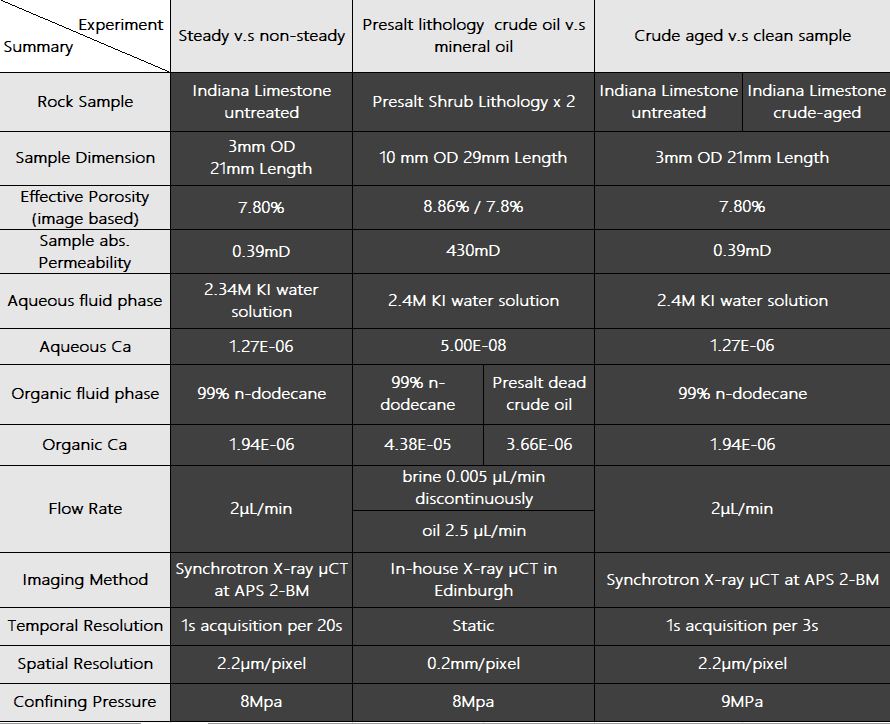
\includegraphics[width=1.2\textwidth]{\dir/figs/exps.png}
  \caption{Table: Summary of experimental conditions}
  \label{exps}
\end{figure}

\section{Experimental set I: Indiana limestone core-flooding experiments imaged with time-resolved synchrotron X-ray microtomography }
\label{2016}
\subsection{Year 2016 synchrotron experiments}
In these experiments, potassium iodide brine and mineral oil (99\% n-dodecane) were used as aqueous and organic fluid phase to perform core-flooding in an Indiana limestone (3mm OD by 21mm length) held in high pressure fluid flow cell 'Sleipnir'. Details of these experiments are listed in Fig.\ref{exps} first column steady v.s. non-steady experiments. These experiments were conducted by Drs Ian Butler and Marina Sousani prior to Yili Yang joined the project.

\subsubsection{Rock}
\paragraph{Indiana Limestone}
In the year 2016 time resolved synchrotron experiments, oolitic Indiana limestone samples were used as the porous rock media. SEM images of the samples (Fig.\ref{sempore}) illustrate two distinct surface topology, the rough, fine grained ooid surface, and the much smoother diagenetic drusy calcite cements surface (red circle in Fig.\ref{sempore}). The pore space magnitude has a wide distribution from under-micron to hundreds of microns. The micro pores that below the synchrotron X-ray microtomography resolution at APS (2.2\textmu m) are sub-resolution porosity that can not be identified by imaging, thus fluid flow inside these micro pores can not be detected and become one of the unavoidable limitations of this experiment. The total sample porosity was estimated of 20.65\% based on the ratio of measured sample density to pure calcite density. The porosity estimated by the ratio of pore to solid based on imaging was 6.5\%. The reasons for this discrepancy, is the sub-resolution porosity that can not be imaged that underestimate the porosity. The actual effective porosity should be higher than 6.5\%. The sample permeability was 0.39 mD, approximately estimated from a measurement of the pressure drop across the sample during loading with water.

The Indiana limestone sample is directly from outcrop and cleaned ultrasonically in de-ionised water in sample preparation.

\begin{figure}[htbp]
  \centering
  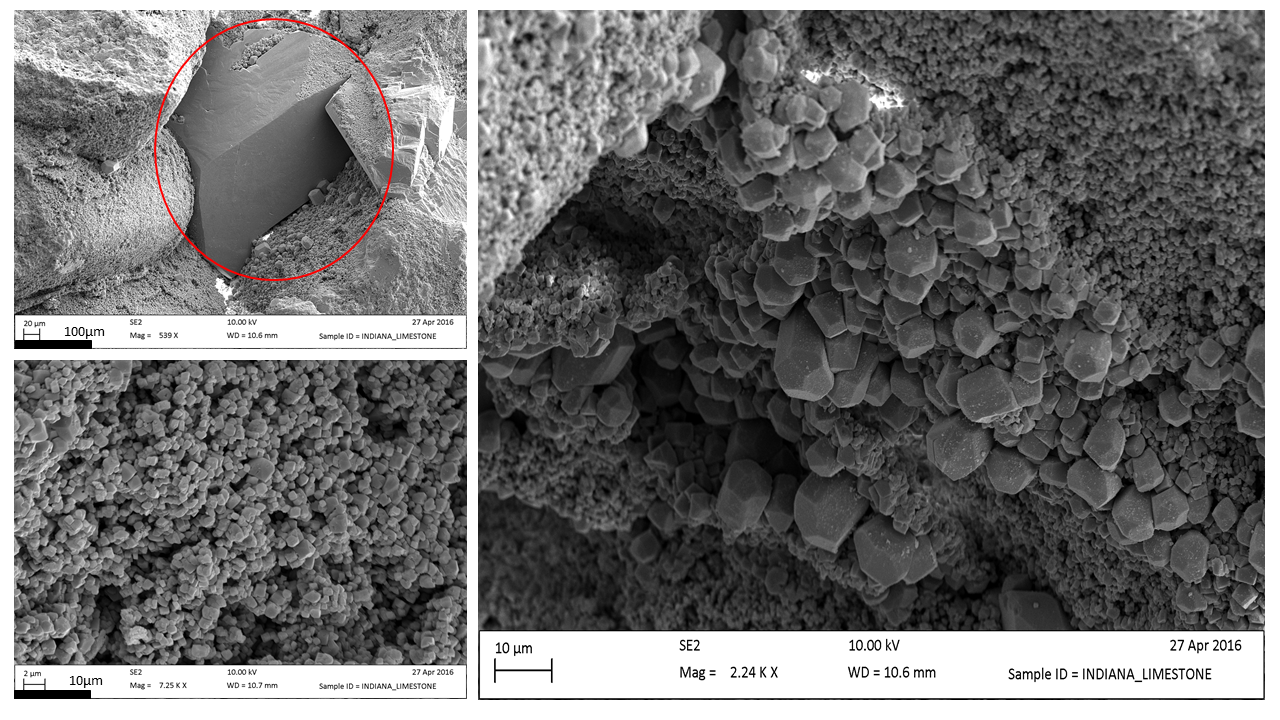
\includegraphics[width=1\textwidth]{\dir/figs/indianapore.png}
  \caption{SEM image of Indiana limestone: core surface with different scales from $100 \mu m - 10 \mu m$. Red circle shows different roughness of the surface. Pores of size close to $2 \mu m$ are close to the resolution of CT imaging used in this study therefore they are micro-pores that leads to underestimation of bulk porosity and uncaptured fluid flow.}
  \label{sempore}
\end{figure}
\paragraph{Core dimension}
The sample used in synchrotron experiments was sized 3mm OD by 21.2 mm length cylinder. The upper 13.7 mm (Fig.\ref{core} grey) was core end zone to exclude capillary effects from the volume of interest. The volume of interest is colored in green in Fig.\ref{core} (target zone), and for the volume above and below the target zone are the buffer zones where static scans were taken.

\begin{figure}[htbp]
  \centering
  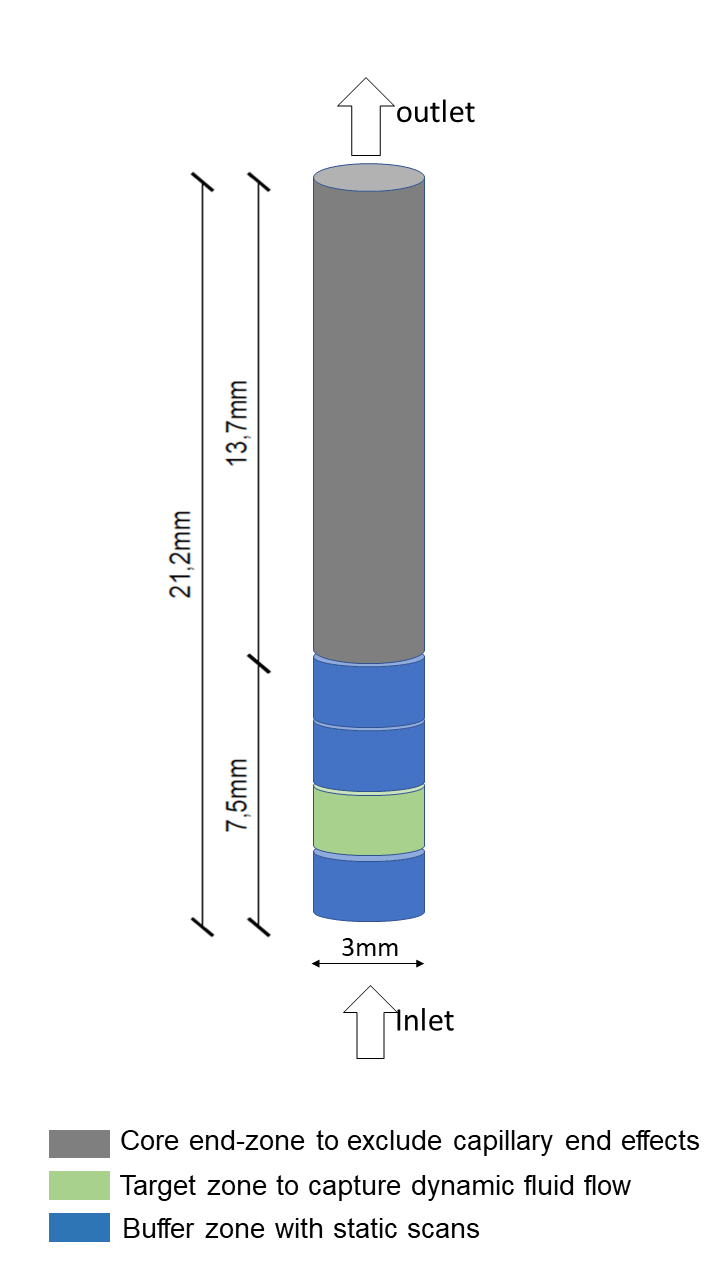
\includegraphics[width=.6\textwidth]{\dir/figs/core.png}
  \caption{Core dimension of Indiana limestone. The core used in the APS 2016 core flooding experiment. The dimension of the cylindrical core is 21.2 mm length $\times$ 3 mm diametre. The grey part of the core is space for eliminating capillary end effect. The bottom four blocks in blue and green are zones that being imaged for fluid flow processes. The blue zones are buffer zones which are imaged with static scans. The green zone is the target zone that imaged with fast scans to capture dynamic fluid flow processes.} 
  \label{core} 
\end{figure}

\subsubsection{Fluids}
\paragraph{Aqueous phase}
The aqueous phase was 2.4M Potassium Iodide (KI) water (deionized) solution. KI is a common doping agent for enhancing the X-ray imaging contrast with oil and rock \citep[e.g.]{iglauer2011residual,culligan2006pore,porter2010measurement}. The viscosity of KI solution at 25$^{\circ}$C is considered as close to water viscosity which is 0.89 MPaS reported by The International Association for the Properties of Water and Steam (IAPWS) 2008. The KI water solution is referred to as 'brine'.

\paragraph{Organic phase}
The organic phase for the synchrotron experiments is n-dodecane (99\%). Its solubility in water at 25$^{\circ}$C is reported to be 8.9 \times 10$^{-10}$ in mole fraction \citep{shaw2006iupac} and can be considered as immiscible with water. The viscosity of n-dodecane is reported in literature to be 1.36 MPaS at one atmosphere pressure and 25$^{\circ}$C \citep{liu2011measurement}. The density of dodecane $\rho=750$ kg/m$^3$ at ambient temperature. The interfacial tension of n-dodecane with water was reported to be 52.8 mN/m at 20$^{\circ}$C \citep{zeppieri2001interfacial}.

\subsubsection{Core-flooding cell}
\paragraph{'Sleipnir' cell}
The core-flooding cell used at synchrotron beamline APS 2-BM was 'Sleipnir' fluid flow cell described by \cite{fusseis2014low} (Fig.\ref{sleipnir2}). The cell was further modified for these experiments to include a carbon fibre composite pressure vessel to enhance X-ray transparency. In addition, the cell was partly re-engineered for zero-dead volume and fluid injections. The Sleipnir cell is capable of sample dimension up to 3mm diameter.

\begin{figure}[htbp]
  \centering
  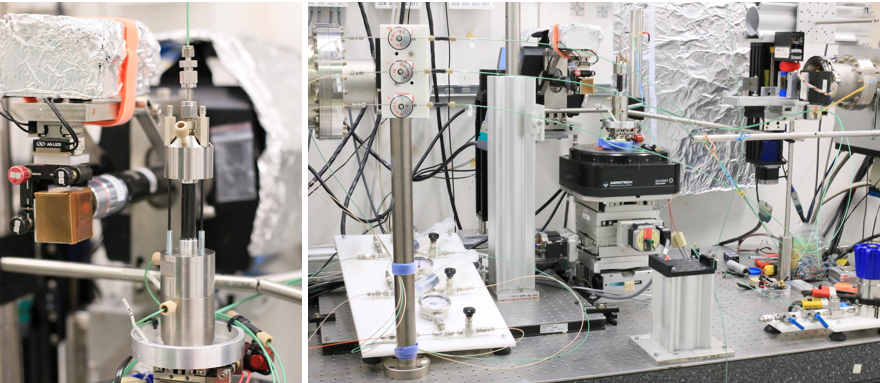
\includegraphics[width=.9\textwidth]{\dir/figs/sleipnir2.png}
  \caption{(Left) Sleipnir cell, with carbon fibre pressure vessel and tie-rods in place on the rotary table in the upstream hutch at 2BM, APS. (Right) Experimental set-up for two phase fluid flow, showing fluid manifolds, high pressure tubing (green). High pressure syringe pumps were located below the optical bench to shield them from scattered radiation. }
  \label{sleipnir2}
\end{figure}

\subsubsection{Core-flooding apparatus}
The experimental apparatus used in synchrotron facility consisted of fluid cell, syringe pumps, isolation valves, and a back pressure regulator (BPR). These components were connected by high pressure tubing and fluid manifolds (Fig.\ref{apparatus}). Three Cetoni neMESYS\texttrademark Syringe pumps were used to inject core-flooding oil, brine and confining fluid (water). The Syringe pumps were precisely controlled by software (Fig.\ref{apparatus} CETONI pumps). Three isolation valves controlled the flow of brine, oil and confining fluid which were leading into the fluid flow cell inlet (Fig.\ref{apparatus} flow cell). And a BPR controls the outlet pressure of the whole system and its outlet led to a waste-fluid bottle. 

\begin{figure}[htbp]
  \centering
  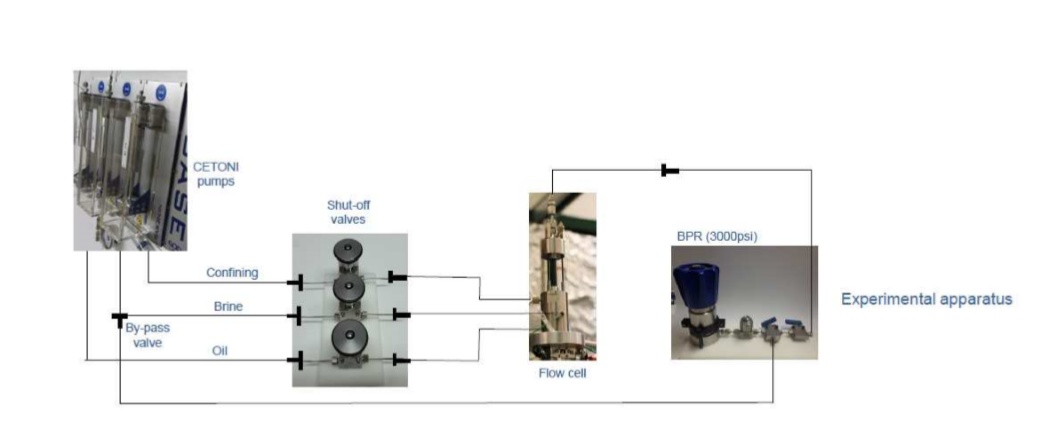
\includegraphics[width=1\textwidth]{\dir/figs/apparatus.png}
  \caption{ Experimental apparatus used at the APS facilities operating multiphase fluid flow experiments under elevated pressure. It consists of three syringe fluid flow pumps, three shut-off valves, a high pressure X-ray transparent fluid cell and a 6000psi back pressure regulator. Figure made by Dr.Ian Butler.}
  \label{apparatus}
\end{figure}

The inlet tube for steady state injections was designed as 'tube-in-tube' (Fig.\ref{design} cartoon) . This design consisted of a inner tube for oil flow and outer tube for brine flow. The design allows both fluids enter the core in a mixed fashion and reduced the impact of the location of accessed pores of fluid phases.

\begin{figure}[htbp]
  \centering
  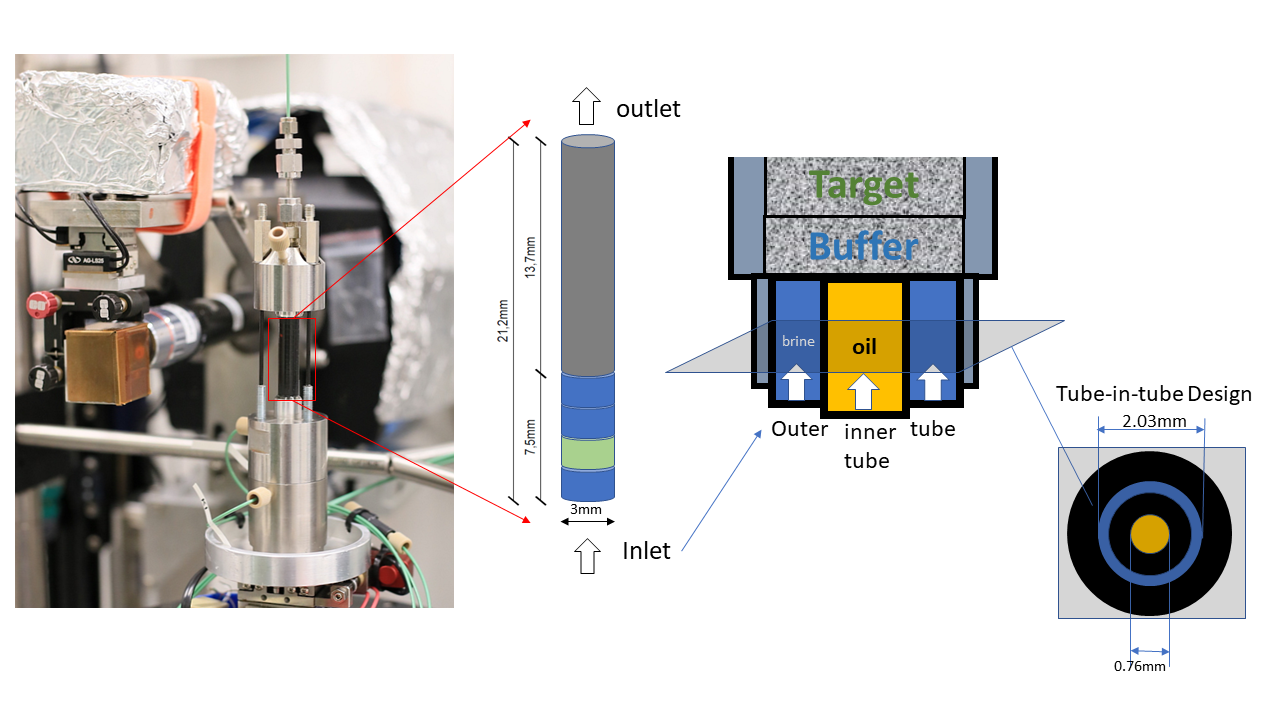
\includegraphics[width=1\textwidth]{\dir/figs/design.png}
  \caption{From left: Sleipnir cell, with carbon fibre pressure vessel and tie-rods in place on the rotary table in the upstream hutch at 2BM, APS. Red box zoomed in shows the carbon fibre vessel that holds the sample core. The inlet was designed tube-in-tube for oil and brine steady state injection. The cross-section of tube in tube design shows its dimension.}
  \label{design}
\end{figure}

\subsubsection{Experimental protocol}
\subsubsubsection{Core-flooding fluid injection sequence}
The Fluid injection sequence during core-flooding is summarised in table Fig.\ref{exptable}. The core before main core-flooding injections was saturated by water, then replaced by brine, then replaced by oil to an irreducible saturation. The experiment had three main stages:

\textbf{1) Brine injection (BI)} Brine injection into oil saturated core (Exp011-Exp015).

\textbf{2) Oil re-injection (OR)} Oil re-injection into brine saturated core (Exp017-Exp019).

\textbf{3) Steady state injection (SS)} Both fluids were injected simultaneously (Exp024-Exp027).

\begin{figure}[htbp]
  \centering
  \includegraphics[width=1\textwidth]{\dir/figs/exp_table.png}
  \caption{Table: Sequence of fluid injections for the elevated pressure experiment}
  \label{exptable}
\end{figure}

\subsubsection{Imaging methods}
The experiments were imaged by synchrotron X-ray radiation at beamline 2-BM Advanced Photon Source (APS), Argonne National Laboratory, US.  This beam line is fully dedicated to fast imaging (second-scale) for slow dynamic phenomena studies. The synchrotron X-ray beam is sourced from the bending magnets that installed on the electron storage ring. The beam energy range is 11-35 keV and the beam size is 25mm x 4mm. Raw projection data was acquired by 2-BM internal code, and reconstructed by python based CT image processing library TomoPy \citep{gursoy2014tomopy}. TomoPy reconstruction is described in detail in the following Data Processing Methods section and TomoPy code written by Yili Yang is attached in the appendices.

The X-ray beam used for imaging is pink beam. Pink beam has narrower energy window comparing with white beam, combined with high photon flux can provide better contrast attenuation than white beam therefore yield higher quality CT images.

Three main injection stages were imaged by fast scans. During fast scan, 600 projections of 180$^{\circ}$ rotation were acquired for each tomogram. The exposure time for each projection was 1.7ms leading to 1s total acquisition time per scan. The gap between fast scans was 20 seconds. The spatial resolution is 2.2 micron per pixel. A total of 140+ CT volumes recording the fluid displacement processes were acquired at the end of experiments.

Multi-position scans were taken before and after each stage to check fluid position and acquire high resolution images. During Multi-position scan, 1500 projections of 180$^{\circ}$ rotation were acquired for each tomogram. The sample was moved vertically to make the x-ray beam scan multiple positions along the long axis of the sample.

\subsubsection{Data processing methods}
\paragraph{Overview}
The overall data processing for X-ray CT data includes reconstruction, segmentation, and post-segmentation analysis. The raw data acquired from X-ray CT are projection images. Reconstruction processes the projections into reconstructed data which are slices of horizontal sections of the object. Segmentation labels reconstructed images by meaningful categories such as pore and solid. The post-segmentation processes analyse the in-depth scientific features of the data. For example, calculates the connectivity of a fluid phase, or count the number and size of oil ganglions, or calculates the pore size distribution of a porous medium.

\subsubsubsection{CT reconstruction} 
The raw data acquired from an X-ray CT scan are the digital signals of attenuated X-ray photons converted into digital images called projections. The projections can be reconstructed to horizontal image section of the object by various of algorithms, e.g. filtered back-projection\citep{kak2002principles} , gridrec algorithm \citep{marone2012regridding,dowd1999developments} etc. By stacking the 2D reconstructed slices, 3D structure of the object can be digitalised.

\paragraph{Octopus}
Octopus\texttrademark is a commercial software for CT image reconstruction \citep{vlassenbroeck2006octopus}. It has a graphical user interface (GUI).  It uses filtered back-projection algorithm to perform reconstruction, and it includes image correction tool kits such as beam hardening correction, normalisation and denoise functions etc. It is user-friendly and faster for small batch of data. The reconstruction time for a CT volume sized $1600 \times 1600 \times 1000$ by Octopus usually takes around 40 minutes on a 16-core workstation. The latest Octopus version enables CUDA GPU acceleration so reconstruction time is massively reduced to few minutes. Octopus was used for the first 20 scans of the 2016 synchrotron experiments.

\paragraph{Tomopy}
TomoPy is an open-sourced software for CT image reconstruction \citep{gursoy2014tomopy}. It is python code based and does not have a GUI. The reconstruction functions include 13 major algorithms for instance filtered back-projection, Fourier grid-reconstruction, algebraic reconstruction and maximum-likelihood expectation maximization algorithm etc. It also includes other image correction functions such as auto centre finding, stripe removal functions, denoise filters and morphology functions. Because it is python based, it has several merits. First it is compatible with HDF files which is the standard data format for synchrotron data, while Octopus can not open. Second it allows user-defined pixel-wise operation, for the purpose of examining and fixing imaging errors. Thrid, it is compatible with other python software, like Open-CV \citep{opencv_library} and Scikit-image \citep{scikit-image}, to incorporate more useful functions and compose the best possible image processing work flow for unique data set. Fourth, it enables automatic batch processing that can loop different files in different folders and processing all-at once, which can save significant processing time. Fifth, it enables seamless subsequent processing of segmentation and scientific analysis using python.

Some parts of the synchrotron CT raw data have blank reconstruction slices, they were due to non-positive pixel values in the projection slices. During reconstruction, the values were proceeded as not-a-number (NaN) value when calculating minus-log function. The NaN value would raise problem resulted as blank slice. This problem was fixed by replacing all the non-positive value pixels in the projections by an extremely small positive number 1$^{-9}$.

The average reconstruction time for a CT volume sized $1600 \times 1600 \times 1000$ took less than a minute on a 32-core workstation. The majority of the synchrotron data was reconstructed by TomoPy. The TomoPy reconstruction code developed by Yili Yang can be found in the Appendices.

\subsubsubsection{preprocessing}
Raw CT reconstruction images usually have artefacts including noise, beam hardening and ring artefacts etc that make segmentation difficult. It is a common practice to pre-process the raw CT reconstruction images before segmentation to reduce the artefacts, thus to improve image quality and lead to better segmentation result. 

\paragraph{Cropping} The first step of pre-processing is cropping. Cropping is to re-size the raw image into the region of interest (ROI), and exclude the irrelevant background regions. Cropping can significantly reduce the processing time and computing resources needed, therefore it is the foremost step of all processing steps.

The following processing depends on the types of artefacts presented on the images. The common artefacts are random noise, ring artefacts, streak/stripe artefacts, beam hardening etc.

\paragraph{Noise} Random noise is the most common artefact, it is inevitable but relatively easy to be filtered. The reason of random noise can be various such as the fluctuations inherent in the detection of a finite number of x-ray quanta, additional signals created by electronic circuits during signal processing, or the round-off errors arise from binary computation \citep{hanson1981radiology}.

\paragraph{Non-local Means filter} 
In chapter two, a classical spatial filter, median filter is introduced. A more advanced filter, the non-local means (NLM) filter \citep{buades2011non} adopted the similar idea, but it replaces the given pixel with the weighted average value of the resembling pixels across the whole image, instead of the median of the peripheral pixels, because '\textit{the most similar pixels to a given pixel have no reason to be close at all}'. The resemblance is evaluated by comparing a square neighbourhood around each pixel, with intensity values and geometrical configuration both taken into consideration. The pixels on the boundary of objects are not averaged by their surrounding pixels, but restored by the pixel value with similar pattern - also on the boundary, therefore the noise is reduced meanwhile the boundaries are preserved. The mathematical expression of NLM is described as following equation:

$$NL[v](i)=\sum_{j\in i}w(i,j)v(j)$$

For pixel $i$ in noisy image $v$, the filtered pixel value $NL[v](i)$ is computed as the sum of weighted average of all resembling pixels $j$. The resemblance of $i$ and $j$ is measured as a decreasing function of the weighted Euclidean distance of their neighbouring values, meaning that the pixel with more similar neighbourhood has higher weight in the average. See \cite{buades2011non} paper for the complete mathematical description of the algorithm.

To compare the noise reduction performance on experimental CT data in this study, seven different filters are tested - the bilateral filter, total variation filter, Gaussian filter, Kuwahara filter, mean filter, median filter and non-local means filter. Non-local means filter has the best performance preserving edge features and noise reduction. And NLM filter has been widely implemented in ImageJ, Avizo\texttrademark and Scikit-image.

\begin{figure}[htbp]
  \centering
  \includegraphics[width=1\textwidth]{\dir/figs/denoisecompare.png}
  \caption{Comparison of denoising by NLM and median filter}
  \label{denoisecompare}
\end{figure}

Fig\ref{denoisecompare} shows an example of comparison between NLM and median filter. The NLM filter has better performance on the example noisy image for less noise while preserving the sharpness of the phase boundaries. In Dr Tannaz Pak's PhD thesis \citeyear{Pak2014thesis}, she reported the comparison of median filter, anisotropic diffusion filter and NLM flter shows that NLM filter has the lowest standard deviation and the narrowest distribution peak in histogram. This confirmed the advantages of NLM filter for multiphase fluid flow experimental CT data in terms of noise removing while preserving phase boundaries.

Besides noise, a range of CT artefacts can be produced during the complex physical process and computing process of microtomography. Beam hardening , streak artefacts and ring artefacts can be alleviated by applying filtering algorithm during reconstruction. 

\paragraph{Intensity normalising} Synchrotron CT reconstructions can have problem that one CT volume have varied intensity along the vertical axis, i.e. some slices are overall brighter than others, and the degree of brightness varied across slices. This problem was fixed by normalising slices by their range of intensity.

$$ nmI(i)=\frac{i-I_{min}}{I_{max}-I_{min}}*a$$

In image $I$, the normalised pixel $nmI(i)$ of original pixel $i$ is calculated as the fraction of the intensity portion and the intensity range of image $I$. $I_{min}$ and $I_{max}$ are the minimum and maximum intensity in image $I$. The intensity portion of pixel $i$ is the difference of pixel value $i$ with the minimum intensity $I_{min}$. The intensity range is the difference of maximum and minimum intensity. $a$ is a coefficient, when $a=1$ the normalised output image format is floating point ranged from 0-1. When $a=255$ the normalised output image format is 8-bit unsigned.

In the 2016 synchrotron experiments, the contrast between the solid phase and aqueous phase is subtle, even with 2.34M KI contrast enhance doping added to the aqueous phase. In order to segment the image, a masking pre-process was applied. A binary segmentation of soild and pore space was extracted from the reference scan at time zero. The segmentation of solid was employed as a mask for the subsequent segmentation of multiphase fluid flow process. (img) 

\subsubsubsection{Segmentation} 
Accurate and efficient image segmentation is the crucial prerequisite of quantitative analysis on CT images. Image segmentation is to assign meaningful labels to digital images pixel-wisely, for example giving each pixel a label of oil, brine or solid to a multiphase fluid flow core-flooding X-ray image. Due to great amount of CT data produced in the experiments and the complexity of the image pattern, it is impossible to manually segment the images. Therefore it is crucial to find an accurate and efficient method to segment CT images.

Conventional segmentation algorithms such as Otsu thresholding \citep{otsu1979threshold} or watershed segmentation \citep{serra1983image} are widely used in the image processing of multiphase flow experiments \citep[e.g.]{andrew2015imaging,singh2016imaging}. In this study, a more advanced algorithm - Seeded Random walker (RW) segmentation \citep{grady2005multilabel} is employed to segment the experimental CT reconstruction images. Random walker is a region growing algorithm similar with watershed, but with better performance in terms of accuracy and efficiency, it also provides probability map for a quantitative evaluation of the segmentation reliability.

\begin{figure}[htbp]
  \centering
  \includegraphics[width=1\textwidth]{\dir/figs/rw.png}
  \caption{An illustrative example of a random walker segmentation (a) modified by Dr Ian Butler from Grady (2006). In this example Grady (2006) uses fixed nodes connected by resistors, with the marker nodes, L1, L2 and L3, alternately (b, c, \& d) representing nodes fixed to a potential of 1 and all resistors were set to the same value. The electric potentials calculated represent the probability that a random walker starting at each node first reaches the seed point currently set to unity. The colour codes indicate which nodes with the highest values “belong” to which marker point, and the final segmentation is shown in (a) as the red line. Translating this example to the case of an image, each resistor would represent a function of the grey scale gradient in the image}
  \label{rw}
\end{figure}

\paragraph{Random Walker Segmentation}
The seeded random walker algorithm was motivated by placing small number of user-defined labels (seeds) that unequivocally belong to a particular phase (i.e. solid), and perform random walk from pixels then noting which seed they first arrive at. Random walk is one of the famous problem scenario in probability theory that a man walking on a street and making turn by probability, and well known for its equivalence with electrical circuits \citep{doyle1984random}. In this algorithm, random walk is performed at each unclassified pixel and noting the probability that they arrived at each seed, and is categorised to the seed with the highest probability. The mathematical problem was solved by combining probability theory and circuit theory on a graph. The image structure was represented by a function that map pixel intensity to edge weights that affect random walker's choice.  

Fig.\ref{rw} shows the analogue of random walker segmentation to electric circuits: the electrical nodes (pixels) are connected by resistors (weights) to the voltage source (seeds) L1, L2, L3 in (a). By solving the probability problem with the aid of circuit theory, the electric potentials (segmentation probability) is computed, and the segmentation is determined by the highest probability.

Random walker algorithm is highly robust that unlikely suffer from the three usual problems in CT image segmentation 1)corrupted image with noise and artefacts, 2)different objects with low contrast or absent boundaries and 3)ambiguity of labels when they are fewer than constant regions. 

\begin{figure}[htbp]
  \centering
  \includegraphics[width=1\textwidth]{\dir/figs/rwresult.png}
  \caption{Random walker segmentation example result}
  \label{rwresult}
\end{figure}

Fig.\ref{rwresult} shows the original reconstructed CT image and the random walker segmentation result that separating pore space and solid. Zoomed-in red box on the original image shows The global thresholding result, blue speckles are the pixels with intermediate intensity that can not be thresholded. The random walker segmentation shows a sharp and clean segmentation of the pore and solid, this high quality segmentation is used as mask for the segmentation of experimental data with two fluids present in the pore space.

Fig.\ref{segworkflow} shows the work flow of segmentation. The raw image is severely suffered from noise and the contrast between solid and brine is poor. By applying mask obtained from Fig.\ref{rw} on the raw image, the masked image shows the to-be-segmented pore space saturated with oil and brine. By applying non-local means filter, the noise is massively reduced and ready for RW segmentation. The seeds are determined by histogram, and the final segmentation is performed by seeded RW implementation in Scikit-image. The segmentation code developed by Yili Yang is attached in the Appendices chapter. The processing work flow took average one hour for each CT volume sized $1646 \times 1646 \times 1004$. A total of 140 plus volumes of synchrotron CT data was segmented using this method.

\begin{figure}[htbp]
  \centering
  \includegraphics[width=1\textwidth]{\dir/figs/f.png}
  \caption{Segmentation work flow}
  \label{segworkflow}
\end{figure}

Fig.\ref{seg2} shows a comparison of the same slice before and after injection, and the segmentation result of injection fluids. Left image shows the reference water-saturated core prior to experimental injection, the image was acquired from static scan which has higher resolution than fast scans. A precise segmentation of solid and pore space is acquired from this image. Middle image shows the fast scan image of the same slice during brine injection. The fast scan achieved high temporal resolution at the cost of compromised image quality. The fast scan image has more noise and horizontal stripe artefact, more importantly, the contrast between brine and solid is so poor that can be barely visually identified. After the segmentation work flow, accurate segmentation of the two fluid occupied pore space and solid is shown on the right. 

\begin{figure}[htbp]
  \centering
  \includegraphics[width=1\textwidth]{\dir/figs/seg2.png}
  \caption{Segmentation result}
  \label{seg2}
\end{figure}

The RW segmentation probability map is shown in Fig.\ref{probmap}. It visualise the probability distribution of all pixels on a image belong to a particular phase. The original image is shown on the left, middle and right images are the segmentation probability distribution of solid and pore space (filled with H$_2$O) respectively.
The colour map is scaled from 0-1 from colour cold to warm. For the probability value of each pixel on the map, the more close to 0 means the lower likelihood that it belongs to the target phase and vice versa. The uncertainty lies in those pixels with likelihood around 0.5, meaning that it is hard for the algorithm to decide whether this pixel belongs to a particular phase or not. The maps in Fig.\ref{probmap} show a very robust segmentation with many determined pixels and only few uncertainty.

\begin{figure}[htbp]
  \centering
  \includegraphics[width=1\textwidth]{\dir/figs/probmap.png}
  \caption{Probability map produced by random walker algorithm}
  \label{probmap}
\end{figure}

Accurate segmentation of CT images guarantees that experimental phenomena are honestly digitalised. Only then can we analyse the physical process presented in the experiments. 

\subsubsection{Post-segmentation image processing}
\subsubsubsection{Fluid connectivity estimation using Euler characteristics}

To study the connectivity evolution of fluid phases during displacement, Euler characteristics ( Euler--Poincar\'e characteristic) is employed as a measurement of topological connectivity of fluid phases. 

The topological definition for a three-dimensional object can be described using Minkowski functionals (details see \cite{blunt2017multiphase,mecke2005fluids}). There are four functionals: M$_0$ the volume of the object, M$_1$ the total area of the object surface, M$_2$ the average curvature on the surface and M$_3$ the total curvature of the surface. M$_3$, unlike the first three functionals, is dimensionless and related to the Euler characteristic $\chi$, which describes the relationship between the number of edges, faces and vertices of a polyhedron,

$$\chi = V-E+F-O$$,

where V is the number of vertices, E the number of edges, F the number of faces and O the number of discrete objects. To relate $\chi$ to the measure of connectivity, this relation is generalised \citep{serra1986introduction,vogel2001quantitative,vogel2002topological} to: 

$$\chi=\beta_0-\beta_1+\beta_2$$,

where $\beta_0$ is the zeroth Betti number referring to the disconnected discrete regions of the object, in the context of this study $\beta_0$ is the individual fluid ganglions and clusters. $\beta_1$ is the first Betti number referring to redundant handles or loops that can be eliminated without breaking the connectivity, quantified by $\beta_0$ staying constant. In the experimental context $\beta_1$ is the pores multiply interconnected by throats. $\beta_2$ is the 2nd second Betti number referring to isolated regions surrounded inside the object. In the experimental context it is the non-wetting fluid completely trapped in a pore surrounded by the wetting fluid.

The Euler characterestics (simplified as Euler number) for the fluid phases were computed using Avizo9\texttrademark. The Euler number is normalised with fluid volume to characterise the unit volume connectivity of the phase.

\subsubsubsection{Pore size distribution}
Pore size distribution (PSD) is an important characteristic of a porous medium. It describes the pore population in relationship with pore width in a porous medium. The PSD of a porous medium can be experimentally determined using many methods including molecular adsorption method (molecular resolution porosimetry), small angle X-ray scattering, mercury porosimetry, nuclear magnetic resonance, thermoporosimetry, liquid extrusion porosimeter, size-exclusion chromatography, water vapor desorption isotherms etc \citep{kaneko1994determination, yang2009image}. From an image-based perspective, PSD can be determined by max ball method or porosimetry simulation etc \citep[e.g.]{delerue1999new,yang2009image,gostickporespy}. 

In this study we used a local thickness approach implemented by \cite{gostickporespy} in python. The algorithm calculates the largest engulfed sphere for each voxel in an image and returns a copy of that image with the pore size value in each voxel. With this image mapped with pore size value, we can plot the PSD curve for different porous media. 

\begin{figure}[htbp]
  \centering
  \includegraphics[width=1\textwidth]{\dir/figs/localthickness.png}
  \caption{Visualisation of maximum engulfed sphere in 2D and 3D}
  \label{localthickness}
\end{figure}

Fig.\ref{localthickness} left shows an image slice produced by local thickness function, the pores are filled with spheres that indicate the maximum radius of that pore, and PSD of the 3D porous medium can be plotted from all the slices. Image on the right shows the 3D rendering of pores with certain size range rendered with red, pores out of this range are not rendered and transparent.

\subsubsubsection{Pore throat-body partitioning}
The size of pore is a fundamental control on the fluid flow process. According to the Young-Laplace equation, it is more energy favourable that wetting phase occupying the narrowest regions first, which means the throats are easy to flow and the pore body impedes the flow. And vice versa for non-wetting phase. In order to know the wettability of the porous medium, as contact angle measurements for every throat that fluids were passing by is not easy, it is more practically feasible to compare the size of pores that fluids were passing by to estimate the wettability.

In this study I established a method to compare the throat size that passed by a fluid with those unpassed throats quantitatively. If a fluid phase passed more larger throats than smaller throats, this fluid phase is generally non-wetting to the porous medium, and vice versa.

\begin{figure}[htbp]
  \centering
  \includegraphics[width=1\textwidth]{\dir/figs/partitionwf.png}
  \caption{Pore body-throat partitioning work flow}
  \label{partitionwf}
\end{figure}

The method work flow is shown in Fig.\ref{partitionwf}. First the raw CT image (1) is denoised (2), and segmented into a binarilised pore space (3). Then Euclidean distance map (4) of the pore space is computed, which is the Euclidean distance of a pixel to its nearest boundary, i.e. the distance of a point inside the pore to the closest rock surface. This distance map is then thresholded using Niblack thresholding \citep{niblack1985introduction}, to find the local maxima of the distance map. The local maxima represent the widest areas locally, which are pore bodies. The unthresholded area in (5) are the throats, the narrowest areas locally. By applying random walker probability map to (5), throats are labelled with the likelyhood of belonging of its nearest pore body (6). 

\begin{figure}[htbp]
  \centering
  \includegraphics[width=1\textwidth]{\dir/figs/throats.png}
  \caption{3D rendering of brine passing throats labelled in colour}
  \label{throats}
\end{figure}

Fig.\ref{throats} visualised the brine inside the oil saturated pore and the pore bodies and throats are rendered from cold to warm colour. This allows a intuitive observation of sizes of throats and pores that fluids were passing.

The most important application of this method is to quantify the size of throats that fluids were passed or unpassed (Fig.\ref{throatsize}). By comparing two adjacent scans in a time series, the throats that connected with the fluid occupation can be examined if they were passed or not. In this figure of throat size distribution, brine passed throats (green) has a positive offset with unpassed throats (red), meaning that brine favours larger pores in general, but still passed some smaller throats, indicating that for the examined region, the porous medium is largely non-wetting to aqueous phase.

\begin{figure}[htbp]
  \centering
  \includegraphics[width=1\textwidth]{\dir/figs/throatsize.png}
  \caption{Passed and unpassed throat size distribution}
  \label{throatsize}
\end{figure}

\subsubsubsection{Modelling of a Roof-snap off event}


%%%%%%%%%%%%%%%%%%%%%%%%%%%%%%%%%%%%%%%%%%%%%%%%%%%%%%%%%%%
\subsection{Year 2017 synchrotron experiments}

In these experiments, brine and mineral oil (99\% n-dodecane) were used as aqueous and organic fluid phase to perform core-flooding in a crude-aged Indiana limestone and an unaltered Indiana limestone (3mm OD by 21mm length). The aim of these experiments is to compare the fluid flow process in crude-aged and unaltered carbonates. Details of these experiments are listed in Fig.\ref{exps} third column.

\subsubsection{Rock}
The cores used in this experimental series are sub-sampled from the same Indiana limestone main sample used in year 2016 synchrotron experiments. Detailed description of this sample see section \ref{2016}.

One Indiana limestone sub-sample was aged with crude oil from Presalt Lula Field to alter its wetting properties. Dead crude oil was introduced into the sample by micro-centrifugation, the oil-covered sample was then kept for 54 days at 75$^{\circ}$C. The pore surfaces can adsorb polar components in the crude oil and thus change its wetting properties \citep{buckley1998mechanisms}. This sample is referred to as crude-aged sample. Another Indiana limestone sub-sample remained untreated as control group, and referred to as unaltered sample.
\subsubsection{Fluids}
\paragraph{Aqueous phase}
The aqueous phase used was the same KI solution as year 2016 synchrotron experiments.
\paragraph{Organic phase}
The organic phase used was the same n-dodecane (99\%) as year 2016 synchrotron experiments.
\subsubsection{Core-flooding cell}
The core-flooding cell used was the same cell 'Sleipnir' used in year 2016 synchrotron experiments, except that the tube-in-tube and zero dead-volume injection design was abandoned.

\subsubsection{Core-flooding apparatus}
The core-flooding apparatus used was the same as year 2016 synchrotron experiments.
\subsubsection{Experimental protocol}
\subsubsubsection{Fluid injection sequence of unaltered Indiana limestone sample}
1) H$_2$O flood and brine saturated pre-injection

2) Dodecane injection 

3) Brine re-injection
\subsubsubsection{Fluid injection sequence of crude aged Indiana limestone sample}   
1) Dodecane saturated pre-injection

2) Brine injection

In the crude-aged sample experiments, data acquisition was halted after step 2)brine injection due to camera malfunction, we were unable to continue with further injections.


\subsubsection{Imaging methods}
The technical aim of the experimental suite is to achieve higher temporal resolution synchrotron micro tomography than 2016. We imaged the experiments in beam line 2-BM Advanced Photon Source (APS), Argonne National Laboratory, US. 

Imaging was performed using pink beam radiation. High quality reference scan of 1500 projections was acquired pre-injetion. The dynamic process of fluid flow was imaged by fast scan of 600 projections through a 180$^{\circ}$ rotation in one second. The interval between each scan was 3 seconds, which is seven times faster comparing with the 20 seconds interval achieved in 2016.  The rotation of the rotary stage, where the sample was mounted, is synchronised with the camera. This allows data acquisition during the rotation of the sample in clockwise and anticlockwise, rotational acceleration and de-acceleration. Zero-dead volume tube-in-tube fluid delivery method using in 2016 was abandoned to minimise the tubing attached which can block the beam. In total over 500 \textmu CT volumes were acquired. 

\subsubsection{Data processing methods}
\subsubsubsection{CT Reconstruction}
Raw CT projections were reconstructed by applying Tomopy CT reconstruction script developed by Yili Yang.

%#################################################################################
\section{Experimental set II: Presalt lithology core-flooding experiments imaged with in-house X-ray microtomography}

In these experiments, brine, mineral oil (99\% n-dodecane) and crude dead oil from Presalt Lula field were used to perform core flooding in a Presalt shrub lithology sample core, held in cell 'Slidr'. The experimental details are summarised in Fig.\ref{exps} second column.

\subsubsection{Rock}
Presalt shrub lithology sample F4402H (Soxhlet cleaned) from Lula Field was cored into two cylinder sub-sample cores of 10mm OD and 29mm length (Presalt Lula LL-1D-RJS, Depth: 5073.35 m, Absolute Permeability: 430 mD, Effective Porosity: 7.8\%; Density: 2.7 g/cm$^3$). Two sub-samples were cored from this main sample to perform dead crude oil injection and mineral oil injection.

\subsubsection{Fluids}
\paragraph{Aqueous phase}
The same KI solution as year 2016/2017 synchrotron experiments was used in this experimental set.

\paragraph{Organic phase}
Dead crude oil from Presalt Lula Field was used in the Presalt shrub lithology sample F4402H experiments using in-house X-ray \textmu CT. Dead oil refers to oil that has lost its volatile components. Interfacial tension of this dead crude oil with water was estimated to be 20 mN/m by Dr.Surmas Rodrigo from Petrobras. Viscosity (NS/m$^2$) at 20$^{\circ}$C is estimated to be 0.043 by curve fitting Petrobras lab measurements at higher temperatures (Fig.\ref{viscosity}).

\subsubsection{Core-flooding cell}
\paragraph{Cell 'Slidr'}
The large sample core-flooding cell (Fig.\ref{largecell3}) is known as ICCR microtomography flow cell 'Slidr', comparing with Sleipnir, can accept sample dimension up to 10mm OD and 40mm length and elevated pressure. We used this cell for larger samples imaged by Edinburgh in-house X-ray \textmu CT. This cell is made of carbon fibre and steel. It has been tested to 20MPa (3000 psi) confinning pressure and designed parameters indicate safe operation up to 35Mpa. Its dimension enables larger sample size thus can study more heterogeneous carbonate rocks. The cohesion material used in this core constrains the temperature limit to 40$^{\circ}$C. The cell was designed by Dr. Ian Butler and manufactured in the workshop in School of Geoscience, University of Edinburgh.

\begin{figure}[htbp]
  \centering
  \includegraphics[width=.9\textwidth]{\dir/figs/largecell3.png}
  \caption{(Left) The flow cell ‘Slidr’ installed on the rotary table of the University of Edinburgh’s micro-tomography instrument. (Middle) Cross section through the cell and cell stand. The cell uses a tube in tube design to enable confining and pore fluid access via the end caps. (Right) The bill of materials for the cell. Stainless steel (316) offers excellent machine ability and corrosion resistance, however CP2 titanium is an alternative that would offer sufficient strength and corrosion resistance and reduce the overall mass of the cell.}
  \label{largecell3}
\end{figure}

\subsubsection{Core-flooding apparatus}
The experimental set-up was as illustrated in Fig.\ref{inhousect} and conditions were confining pressure = 80 bar (8 MPa), and fluid outlet pressure was set using a back pressure regulator to 53 bar (5.3 MPa). All processes were conducted at ambient temperature.

\begin{figure}[htbp]
  \centering
  \includegraphics[width=.9\textwidth]{\dir/figs/inhousect}
  \caption{Experimental set-up for core-flooding experiments. Image adapted from ICCR final report 2019.}
  \label{inhousect}
\end{figure}

\subsubsection{Experimental protocol}
\subsubsubsection{Fluid injection sequence using dead crude oil}
The overall experimental sequence is summarised as follows: 

1) Water saturated scan pre-injection

2) Displace water with brine 

3) Brine saturated scan 

4) Dead crude oil injection for 4 pore volumes (2.5 \textmu L/min) 

5) Dead crude oil saturated scan 

6) Brine re-injection (0.005 \textmu L/min discontinuously)

7) Multiple scans, partially brine to saturated conditions

The first set of experiments the oil used is dead crude oil from Presalt Lula field. During Brine re-injection (step 6), displacement of previously injected dead crude oil by brine resulted in a significant inlet pressure rise, even when flow rates were reduced to the minimum rate of the pump (0.005\textmu L/min). We had to halt brine injection when inlet pore fluid pressure approached 70 bar, and waited for inlet pressure slowly reduce. The reason of this pressure rise is currently unknown, it may related to the temperature we were performing. According to Dr Surmas Rodrigo from Petrobras, this dead crude oil can flow smoothly in the core in elevated temperature around 70$^{\circ}$.

\subsubsubsection{Fluid injection sequence using mineral oil}
Subsequent experiments on the same lithology used 99\% n-dodecane as a mineral oil. Flow rate of 2.5 \textmu L/min of both fluids maintained throughout the experiments, which was equivalent to a bulk capillary number of $Ca ~ 10^{-9}$. 

1) Water saturated scan pre-injection

2) Displace water with brine 

3) Brine saturated scan 

4) Mineral oil injection for 4 pore volumes

5) Mineral oil saturated scan 

6) Brine re-injection

7) Multiple scans, partially brine to saturated conditions

\subsubsection{Imaging methods}

The experiments were imaged by the X-ray \textmu CT facility in the University of Edinburgh (Fig.\ref{edinburghxray}). X-ray voltage used was 120 kV peak energy that ensures a significant proportion of the produced keV spectrum spans the iodine k-edge, which is the binding energy of the innermost electron of iodine, to activate a sudden increase of attenuation coefficient, resulting in excellent X-ray contrast of the data. Each scan took about 40 minutes to finish thus only the start and terminal status of each fluid injection were captured. CT instruments specifications are listed as follows:

\begin{itemize}
 \item X-ray source (Feinfocus FXT-160.48-2, dual head transmission/directional nano/microfocus tube), with spot size of 12 ± 1 μm for X-ray energy of 120 keV. 
 \item X-ray camera :4 MP Gadox X-ray camera (Rad-icon Shad-O-Box)
 \item Air-bearing rotary table (Micos UPR-160F SMC pegasus with taurus motion controller)
\end{itemize}

\begin{figure}[htbp]
  \centering
  \includegraphics[width=1\textwidth]{\dir/figs/edinburghxray.png}
  \caption{ECOSSE X-ray μCT scanner components: (A) X-ray source (Feinfocus dual head transmission/directional nano/microfocus tube), (B) Air-bearing rotary table (Micos UPR-160F SMC pegasus with taurus motion controller), and (C) 4 MP Gadox X-ray camera (Rad-icon Shad-O-Box)}
  \label{edinburghxray}
\end{figure}

Projection data was acquired via a local C++ code and operated via a Testpoint (V.6) Shell program to coordinate the table rotation with image sensor.

Subsequent image reconstruction was performed via Octopus\texttrademark. The high grey scale contrast between brine and crude or mineral oil enabled direct thresholding segmentation of discrete fluids and rocks. Data analysis and visualisation were using Avizo9\texttrademark and ImageJ software.

%##################################################################################


% \renewcommand{\dir}{../chapter4/chapter/}
% \chapter{Application of Deep Learning in Segmenting Experimental Core-flooding Microtomography Images}
\section{Introduction}
The segmentation work flow described in Chapter 3 works well on the data in terms of quality, but it has some shortages. First, it has three main steps which are denoising, masking and segmentation, each step has few adjustable parameters, it is very time consuming to test the parameter combination for the best segmentation result in different imaging conditions. So the work flow is not a 'panacea' for all CT data. Second, it relies on the mask image segmented from reference scan, data that lack of such reference and suffer from poor contrast could not be accurately segmented using this work flow. Third, the overall processing time for one synchrotron experiment by the work flow is month-scale, which becomes a bottle-neck for the subsequent scientific analysis. So it is necessary to employ the state-of-art deep learning segmentation using convolutional neural networks (CNN) that can massively reduce the processing time meanwhile yield equally good segmentation.

\section{Deep learning for image segmentation}
Machine learning is a subset of artificial intelligence that can make self-modification through structured data to improve its output. One of the many applications of machine learning is computer vision, i.e. recognising objects from digital images. Image segmentation is one of the main tasks of computer vision. Various of machine learning algorithms have been powering image segmentation, for example from unsupervised K-means clustering \citep{lloyd1982least}, to supervised trainable Weka segmentation \citep{arganda2017trainable}. Deep learning is a more advanced subset of machine learning that use multiple layers of algorithms to create an 'artificial neural network'. With this layered structure of algorithms, machine can use each layer to hierarchically learn specific features of images, and produce better outcome with less human interference. The core of deep learning is the backpropagation algorithm \citet{lecun1989backpropagation} that allows discovery of intricate structure in large data set. Backpropagation uses these information to indicate the self-modification of its internal parameters (neurons) that are used to compute the representation in each layer from the previous layer. With large image data sets provided to deep neural network, machine can learn a computational model that represents the relation between raw image and segmentation, and this model can be used to predict the segmentation of data sets of similar kind.

\subsection{Convolutional Neural network}
CNNs \citet{lecun2015deep} are a class of deep neural network that have been proved effective in segmentation tasks (e.g. \citet{long2015fully}; \citet{krizhevsky2012imagenet}; \citet{girshick2014rich}). CNNs are specialised in processing data that has a grid-like topology, such as an image - digital images comprise arrays of pixels arranged in a grid and each pixel has a value for intensity. 

Convolutional neural network normally consists three kind of layers: convolutional layers, pooling layers and fully connected layers. For example \citet{krizhevsky2012imagenet} built the ground breaking CNN for image classification with five convolutional layers and three max pooling layers with a final fully connected layers. Fig.\ref{cnn} shows the generic architecture of CNN. 

\begin{figure}[htbp]
  \centering
  \includegraphics[width=1\textwidth]{\dir/figs/cnn.png}
  \caption{\citet{bernal2019deep}}
  \label{cnn}
\end{figure}

\subsubsection{Convolutional layer}
Convolution is essentially a mathematical operation on two functions $f(x),g(x)$ to produce the third function $h(x)$. $h(x)$ is the integral of the product of $f(x),g(x)$. In the context of CNN, convolutional layer uses a fixed sized matrix, i.e. a kernel, to operate convolution on a small local part of an image, then produce a feature map that extracting simple features such as edges, curves, corners and color patches (see for example Fig.\ref{featuremap}). The kernel will slide across the whole image and extract such simple features of the image. As the convolution process going, more complex and higher level features, such as eyes, hands are extracted in deeper convolutional layers.

\begin{figure}[htbp]
  \centering
  \includegraphics[width=1\textwidth]{\dir/figs/featuremap.png}
  \caption{Examples of feature map learned by \citet{krizhevsky2012imagenet}. The first convolutional layer is extracting local patterns such as edges and colour patches. The kernel size was $11\times11\times3$ and the image size was $224\times224\times3$. 3 is the channel depth and each represents one of the RGB colours for a coloured image.}
  \label{featuremap}
\end{figure}

\subsubsubsection{Non-linearity layer}
\label{nonlinearity}
Linear classifiers can only distinguish superficial patterns because they can only carve their input space into very simple regions \citep{lecun2015deep}. It may distinguish cats from dogs, but for more complex and sensitive tasks such as distinguish Samoyed dogs from wolves (both look alike but subtly different), non-linear classifiers are more suitable for the job. 
Non-linearity is achieved using a group of functions called activation functions after convolution, such as sigmoid function ($A=\frac{1}{1+e^{-x}}$), Tanh function ($tanh(x)=\frac{2}{1+e^{-2x}}-1$) and rectified linear unit (ReLU, $A(x) = max(0,x)$).

\paragraph{ReLU}
\begin{figure}[htbp]
  \centering
  \includegraphics[width=1\textwidth]{\dir/figs/relu.png}
  \caption{relu}
  \label{relu}
\end{figure}

ReLU is one of the most commonly used activation function in CNN \citep{deng2014deep}, It gives an output x if x is positive and 0 otherwise (Fig.\ref{relu}). ReLU also slim down the network by making the activated neuron sparse and more efficient. Some variants of ReLUs such as LReLU, PReLU, RReLU \citep{xu2015empirical,he2015delving,maas2013rectifier} were also proposed to serve different learning scenarios.

\subsubsection{Pooling layer}
Following non-linear activation functions, the output is modified by a pooling (or subsampling) layer before proceeding to the next convolutional layer. Pooling serves mainly three purposes 1) to reduce the number of parameters, 2)alleviate over-fit and most importantly 3)increase translation invariant (i.e. preserving recognition of objects across variation in position, scale, illumination etc.) \citep{goodfellow2016deep}.

Among many pooling methods, max pooling is one of the most commonly used method. Max pooling is done by sub-sampling the maximum value of non-overlapping sub-regions of the image (see Fig.\ref{pooling} for example).

\begin{figure}[htbp]
  \centering
  \includegraphics[width=1\textwidth]{\dir/figs/pooling.png}
  \caption{pooling}
  \label{pooling}
\end{figure}

\subsubsection{Fully connected layer}
Fully connected layer (FC layer) connects all units of the previous layers. It gives an overview to the complete output image. The output of this layer can be the prediction of class labels, or an intermediate layer for consecutive stacking of FC layers depending on the situation.

\subsection{CNN architecture: U-net}
\label{unet_architecture}
\citet{ronneberger2015u} proved the reliability of CNNs in segmenting neighbouring cells of biomedical images, which has similar difficulty with segmenting experimental multiphase flow images generated by microtomography. For this reason, among various of CNN architectures such as ResNet (\citet{he2016deep}), GoogLeNet (\citet{szegedy2015going}) and VGGNet (\citet{simonyan2014very}, we chose the CNN architecture 'U-Net' introduced by \citet{ronneberger2015u} as the CNN architecture used in this study.

\subsubsection{Network Architecture}
The U-net architecture is demonstrated in Fig.\ref{unet}. Built upon the neural network of \citet{ciresan2012deep}, U-net made improvement on the temporal efficiency, the use of context and the amount of data needed of \citet{ciresan2012deep}'s network.

\begin{figure}[htbp]
  \centering
  \includegraphics[width=1\textwidth]{\dir/figs/unet.png}
  \caption{modified from \citet{ronneberger2015u}}
  \label{unet}
\end{figure}

The network consists of contracting path (Fig.\ref{unet} left box) and expansive path (Fig.\ref{unet} right box). The contracting path, like conventional CNN, uses $3\times3$ convolution, followed by ReLU, then $2\times2$ max pooling for down-sampling. 

The expansive path up-samples the feature map with $2\times2$ up-convolution (the reverse operation of convolution), each up-convolution followed by $3\times3$ convolution with ReLU. A concatenation (joining) of feature map of the corresponding contracting path is applied to the up-convoluted feature map (Fig.\ref{unet} grey arrow copy and crop). The concatenation of cropped feature map from contracting path is necessary for compensating the lost border pixels during convolution. U-net does not have any FC layer, the final $1\times1$ convolution maps the total 64-component feature vectors to the desired number of classes. 

Comparing with \citet{ciresan2012deep}'s network, U-net has more feature channels in the up-sampling part, this allows the propagation of features to higher resolution layers. U-net also allows seamless segmentation of arbitrary size of input image. The original paper provided a Caffe \cite{jia2014caffe} implementation of U-net, in this study I used \citet{Jorispytorch}'s implementation of U-net in Pytorch environment. It has many tweakable options such as: 1) depth of the network, 2) number of filters per layer, 3) transposed convolutions vs. bilinear upsampling, 4) valid convolutions vs padding and 5) batch normalization.



\subsection{Principles of artificial neural network training}
Training an artificial neuron network segmentation model is a supervised learning process. The target of the neuron network model is to segment raw CT images as containing three phases: rock, oil and brine. First we collect a large data set of raw CT images, each image paired with its corresponding ground truth, i.e. the training data set. During training, the model is shown a raw image and produces an output of probability map that each pixel belongs to a specific category. We want the correct pixels have the highest probability than the wrong ones. At the onset of training, the prediction is random and unlikely to be correct everywhere. We use loss function (e.g. cross entropy loss for comparing probability distribution) to measure the error/distance between the output probability and the ground truth. By back-propagating the loss, the model attempts to adjust its internal parameters aiming at reducing the loss therefore make better prediction of the phases. The many internal adjustable parameters, namely neuron weights, are 'knobs' that define the input-output function of the model \citep{lecun2015deep}.

The neuron weights are adjusted using gradient vectors that computed by the machine. The gradient vectors indicate the error increments or decrements brought by tiny changes of neuron weights. A procedure called stochastic gradient descent (SGD) is commonly used to adjust the weights according to the gradient vectors. This is the internal mechanism for deciding how to turn the many 'knobs' of the model to minimise loss. The loss function, or objective function, is a higher-level, averaged representation of neuron weight values. Gradient vectors are indicators of the steepest descent of loss values. The loss values are step-wisely decreased to approach a minimum, where the prediction error is the lowest on average. 

One update of the neuron weights by one image is called a step, one full traverse of the training data set is called an epoch. The full training data set is usually iterated for tens to hundreds of epochs. During training, the loss is continuously reduced and eventually the decrement becomes infinitely small. Upon approaching the loss minimum, the model is well-trained and is then measured on a held-out set of examples, i.e. the test data set, to test the segmentation model's generalisation ability. Unlike the training data set that were 'seen' by the model for many iterations, the held-out testing data set is completely 'unseen' by the model. So the testing, like a mock test to a student, examines the model's prediction performance to unfamiliar real world data. 

\subsubsection{Accuracy evaluation}
The loss functions is more of a measurement of resemblance between input and output during training, it has limited indication of the final segmentation quality. Therefore more direct criteria of segmentation quality are needed to assess the model prediction. The resemblance between prediction and ground truth images is often quantified using intersection over union (IoU, e.g. \citep{rahman2016optimizing}), or receiver operating characteristic \citep{delong1988comparing} functions such as accuracy, precision, recall and F1 score etc. These criteria directly compare two binary images in a pixel-wise way, for example, precision measures the percentage of selected pixels that are correct, and recall measures the percentage of correct pixels that are selected, F1 score is the harmonic mean of precision and recall. These criteria directly indicate the quality of a segmentation. Trained models are tested with a testing data set using the above measurements. 

\subsubsection{Model generalisation and over-fit}
The ultimate goal of neural network training is predicting unfamiliar image segmentation, so a generalised model is crucial for this task. If the model is too specific to a homogeneous type of data, it is unable to make generalised prediction to new input. This problem is generally due to three reasons: 1)the model is trained with inadequate data, 2) the training data is biased, 3) the model is excessively trained with the same data. For inadequate training data, data augmentation strategy \citep{ronneberger2015u} can enlarge limited data set. For biased data set, make more heterogeneous data set can mitigate this problem. For the third situation, the exact amount of training needed for a model is crucial. With training data of suitable size and heterogeneity, if the amount of training is inadequate, the model is under-fit and can not make good prediction. If the amount of training is excessive, the model becomes over-fit and can not make general prediction to new data. Only the right amount of training can produce good model that can produce accurate segmentation to new data.

\begin{figure}[htbp]
  \centering
  \includegraphics[width=1\textwidth]{\dir/figs/VALIDATION.png}
  \caption{}
  \label{validation}
\end{figure}

Validation is a syn-training process to keep track of the amount of training. Unlike training that updates the neuron weights every step and continuously makes improvement to the model, validation only checks the loss of the current model with a smaller data set, the validation data set. Fig.\ref{validation} shows a typical loss curve of training (orange) and validation (blue), the best training point is where the validation loss curve starting to increase (iteration=250), meaning that the model starts to over-fit from that point and prediction becomes less resemble to the ground truth. Stopping training at the validation loss turning point is called early-stopping and is regularly used to prevent over-fit.

\section{CNN training method for segmenting core-flooding experimental X-ray image}
\subsection{Software, functions and hyper-parameters in Training}
\subsubsection{Pytorch}
Pytorch \citep{paszke2017automatic} is an open-sourced deep learning ecosystem that provides tools and functions ready-to-use for deep learning projects. Comparing with other popular deep learning ecosystems such as Google's Tensorflow \citep{tensorflow2015-whitepaper} and UC Berkley's Caffe \citep{jia2014caffe}, Pytorch is more user-friendly, clear and simple in the process of neural network training. Pytorch is flexible and more suitable for small projects and prototyping. For the above reasons I used Pytorch to build the deep learning framework of this study.

\subsubsection{GPU acceleration}
Nvidia\texttrademark QuadroK5200 (8Gb) GPU allows CUDA \citep{cook2012cuda} to parallel computations on GPU and accelerate training. For same heavy computational load, CPU is efficient in complex computation of small amount, and GPU works better with simple computations of large amount, which is the convolution process in CNN training.

\subsubsection{CNN architecture}
U-net was the CNN architecture used in this study. Detailed description of U-net see \ref{unet_architecture}.

\subsubsection{Optimiser: Accelerating training}
Optimiser algorithms are used to accelerate training, there are a number of different built-in optimisers in Pytorch, such as Momentum \citep{sutskever2013importance}, RMSprop \citep{graves2013generating} and Adam \citep{kingma2014adam}. A simple test example of these three optimisers were run following \citet{MofanPython}'s online tutorial, and produced Fig.\ref{optimizer} to compare the performance of them.

\begin{figure}[htbp]
  \centering
  \includegraphics[width=1\textwidth]{\dir/figs/optimizer.png}
  \caption{}
  \label{optimizer}
\end{figure}

The advantage of using an optimiser is to reduce loss faster with less training. Fig.\ref{optimizer} shows RMSprop has the steepest loss reduction in this test and adam has similar effect of reducing loss, and Stochastic gradient descent (SGD, \citet{bottou2010large}), shows the loss reduction rate without an optimiser. I chose Adam as the optimiser to accelerate training because it is the most advanced optimiser among these four, in theory it combines momentum method and RMSprop method together.

\subsubsection{Activation function}
Activation function ReLU was used during training. See \ref{nonlinearity}.

\subsubsection{Loss function}
Pytorch built-in cross entropy loss was used as the loss function during training. It is one of the mostly used loss function for classification problems. Cross entropy loss describes the distance between two probability distributions, i.e. the euclidean distance of probability distribution produced by the network output and the ground truth in the context of this study.

At the first thought, one may wonder why not directly use classification error that measures the percentage of correctly predicted pixels? Because 51\% probability and 99\% probability that a pixel belongs to oil category both show the same result of true positive when use classification error, but the latter model that can make more certain prediction is much better than the former. Here the purpose of using loss function is to find a better model that making more reliable prediction, so we need to compare probability rather than classification.

To understand cross entropy loss, here we dig a bit into information theory. In information theory, the amount of information carried by an event can be quantified by it's probability of happening. For analogue, if one man received an email and he knows all the contents before receiving, the email carries zero information to the man. The man only get information when he knows less than 100\% of the email contents. When the man gets information that previously unknown, he will be 'surprised'. In the segmentation context, the degree of surprise brought by the model prediction 'surprisal' $s$, is calculated by:

\begin{equation}
S=log(\frac{1}{y_{i}})
\end{equation}

Where $y_{i}$ is the $i$th pixel of image $y$, containing information of probability that it belongs to a particular category, for example oil. Now take a weighted average of surprisals of all $n$ pixels of the model prediction, we get the entropy $e$ of this prediction:

\begin{equation}
e=\sum_{0}^{n}y_{i}log(\frac{1}{y_{i}})
\end{equation}

Generally, entropy refers to disorder or uncertainty, Claude Shannon \citep{shannon1948mathematical} used 'information entropy' to measure the amount of information conveyed by each event. In order to compare distance of two probability distributions $q_{i}$ and $p_{i}$, cross entropy $c$ is used:

\begin{equation}
c=\sum_{0}^{n}p_{i}log(\frac{1}{q_{i}})
\end{equation}

It measures the distance of the model prediction probability distribution $q_{i}$ and its ground truth $p_{i}$. Cross entropy $c$ decrease when $q_{i}$ and $p_{i}$ is more alike, and vice versa. By minimising the cross entropy loss, the model can make prediction that most resemble the ground truth. 

\subsubsection{Evaluation Functions}
\paragraph{Receiver operating characteristics }
ROC \citep{delong1988comparing} are measurements of classification errors. First we take probability above 95\% in model prediction as true, then calculate the true positive (TP), false positive (FP), true negative (TN) and false negative (FN) w.r.t. the ground truth. These four numbers can be used to calculate precision, recall, accuracy and F1 score, in this study we only use the Rand accuracy of each phase to evaluate segmentation quality:

\begin{equation}
    accuracy=\frac{TP+TN}{TP+TN+FP+FN}
\end{equation}

The reason for not using precision or recall is that they only take true positive into account but not true negative. The two phase may not necessarily present in every image. For those images that one fluid does not present, the true positive count of that fluid phase equals zero, thus the phase precision/recall is zero and could not represent the true accuracy. F1 is the harmonic mean of precision and recall thus also equals zero for the phase that does not present. In this study I only use accuracy for simplicity although exception can be coded to correct those wrong measurement by precision and recall.

\paragraph{Intersection over Union}
IoU is the ratio of the overlapping area of prediction and ground truth (intersection), with the total area that encompassed by prediction and ground truth (union):

\begin{equation}
    IoU=\frac{Area-of-Overlap}{Area-of-Union}
\end{equation}

A combination of these two metrics can define a good segmentation quality.

\subsubsection{Batch normalisation}
Firstly introduced by \citet{ioffe2015batch}, batch normalisation is a method to reduce internal covariate shift. Internal covariate shift is the change of input distribution to a learning system. Deep neural network amplifies even small changes of input whether relevant or irrelevant, leading to changes of the internal layers of the neural network. Batch normalisation is added before each non-linearity layer to achieve better training outcome.

\subsubsection{Hyper-parameters}
Hyper-parameters are readily defined parameters that control the overall learning process. Such as epochs, batch size, learning rate and regularisation.

\paragraph{Epochs} defines the total training epochs, i.e. the number of iterations to traverse the full training set.

\paragraph{batch size} defines the number of training images that being sent to the network at one step, called a mini-batch.

\paragraph{Learning rate} defines the speed of learning. An appropriate learning rate can make training loss converge within a reasonable training time, and meanwhile prevent divergent of the loss function.

\begin{figure}[htbp]
  \centering
  \includegraphics[width=1\textwidth]{\dir/figs/learninrate.png}
  \caption{}
  \label{learninrate}
\end{figure}

A test example of different learning rate shows in Fig.\ref{learninrate}, learning rate $5^{-5}$ is too low and lead to slower convergence of the loss curve (65000+). Learning rate $1^{-4}$ is appropriate that the loss curve does not diverge and converge faster (20000+) and smoother. For even higher learning rate, the loss will oscillate and hard to converge.

\paragraph{Regularisation} is a method to alleviate over-fitting by penalising high-valued regression coefficients, i.e. it reduces redundant parameters and slim down the model. In this study I used L2 regularisation (or Ridge Regularisation) that penalise the sum of squared weights. There is also L1 regularisation that penalise the sum of absolute values of weights. (The mathematical details of L1 and L2 regularisation is beyond the scope of the context)

\subsection{Data preparation}
A total of 18 CT volumes were used to train the CNN model. Each CT volume consists of raw images of size $1004 \times 1646 \times 1646$ and each paired with the corresponding ground truth images. The 18 CT volumes were split into 14:2:2 for training, validation and testing. A total of 14k+ images were used to train the CNN.

\subsubsection{Ground-truthing}
The ground truth images were segmented by seeded random walker described in chapter 3. 

The deep learning approach applied herein to analyse microtomography data differs from typical CNN application of segmenting objects like, e.g., a cat or a person. In such conventional approaches, training data sets are collections of thousands of manually segmented images. However, manual, genuine ground-truthing for all training data is unfeasible because of the highly irregular, complex, multi-scale or even fractal nature of pore-scale images. 

Thus high-quality microtomographic scans obtained before the initiation of the experiment are segmented using the random walker algorithm and used for training, along with high quality scans of the pore space with two fluids present. The ground truth segmentation images, although are not genuine ground truth, are the best possible segmentation that can be considered as the closest ground truth (Fig.\ref{test_original}). 

\begin{figure}[htbp]
  \centering
  \includegraphics[width=1\textwidth]{\dir/figs/17_test_original.png}
  \caption{}
  \label{test_original}
\end{figure}

\subsubsection{Resizing of raw images}
The images, when loaded into the network, were down-sampled and cropped to $496\times496$. This size is reasonable for our GPU capibility (Nvidia\texttrademark Quadro K5200 8Gb) and the input image size is the multiple of $2^{depth-1}$
which satisfies the sampling process. 

\subsubsection{Intensity normalisation}
The pixel values were normalised to 0-1 using below equation to minimise intensity shift across images.

\begin{equation}
I[i]_{Nj}=\frac{j-I[i]_{min}}{I[i]_{max}-I[i]_{min}}
\end{equation}

where the normalised pixel $Nj$ of image $I[i]$ is calculated by: the difference of the original value of pixel $j$ with the minimum value $I[i]_{min}$ in image $I[i]$, divided by the difference of the maximum value with the minimum value $I[i]_{min}$ in image $I[i]$. It alleviated the intensity shift across images such as image A is overall brighter than image B.

\subsection{Training}
Prior to training, essential python packages for CNN training such as Pytorch \citep{paszke2017automatic}, Numpy \citep{van2011numpy} were imported into Python 3 environment. U-net CNN architecture implemented by \citet{Jorispytorch} was imported as the initial CNN model. 

\begin{figure}[htbp]
  \centering
  \includegraphics[width=1\textwidth]{\dir/figs/workfl.pdf}
  \caption{}
  \label{workfl}
\end{figure}

For one epoch, during each training step a raw image from the training data set was input into the CNN model, and a prediction of the three phase segmentation (oil, water, solid) was then produced by the CNN model. The segmentation was compared with the corresponding ground truth images by the cross entropy loss and yield a training loss value. The training loss was back-propagated to the network and the neuron weights were updated accordingly trying to minimise the loss. The loss gradually decreased as the training went on. The epoch ended when all images in the training set were traversed.

\subsection{Validation}
After each epoch, validation process measured the validation loss of the current model to prevent over-fit. A traverse of the validation data set by the model calculated the current validation loss, but there was no back-propagation of the loss so the model stayed unchanged. The training would proceed to the next training epoch if the validation loss was not increasing. The new epoch would repeat traversing the training data set but with a shuffled input sequence so the way that neuron weights being updated is different.

The best fit model was found at the epoch when the validation loss started increasing, because after this epoch the model started over-fit.

\subsection{Testing}
The trained model was tested using the held-out test data set. Accuracy and IoU was measured from the model prediction to assess the quality of segmentation of unfamiliar data.

\section{Results}
\subsection{Training result}
The CNN model was trained for 34 epochs using the above described methods. Fig.\ref{training_result} shows the loss values and accuracy and IoU measurements evolving through the training process. The total training time was 205.4 hours. 

The upper image shows the validation accuracy of the three phases: oil, brine, and rock (background). And three-phase IoU was also calculated. All measurements have reached above 98\%, and after the 28th epoch the accuracy stopped increasing.

The lower image shows the training loss versus validation loss. Training loss decreased monotonically from 1.1 to 0.02 during training. The validation loss crossed over the training loss at the 18th epoch, after some epochs of further subtle fluctuation, validation started increasing, although of a tiny amount, at the and this figure indicates the over-fit point at the 28th epoch. It is very difficult to identify the validation error increase on the figure because the increment is subtle, the criterion of early stopping was set as validation error increasing for consecutive five epochs. It is sure that the validation error will increase if training continues, I stopped training here because the best-fitting point at the 28th epoch has already been found. The overall decrement of the validation loss was tiny, it is difficult to see the very obvious u-shaped turning point paradigm because the curvature will take unrealistic time to form.

\begin{figure}[htbp]
  \centering
  \includegraphics[width=1\textwidth]{\dir/figs/training_result_23oct}
  \caption{}
  \label{training_result}
\end{figure}

Noticing that the validation loss only changed for a very small amount, and it was already low from the first training epoch. This is because the training data set is considerably large, and the patterns are relatively simple and mostly dependent on its grey value, the model can learn a lot at the first epoch of training. The rest of the training was fine-tuning of the parameters for the very scarce but problematic features.

Another observation worth for attention is that the validation loss is relatively stable, while the training loss kept decreasing. This can be explained by the fact that the training data set is a time series that the adjacent ones are very similar, the validation set is also very similar to the training set which has the adjacent time stamp to it, thus the network learned well. However the validation set is very different from the early time stamps, so the later part of the training was spent on learning these trans-timestamp differences.

In the accuracy plot, the IoU curve (purple) is almost overlapping with the solid (blue), this is a coincidence due to the nature of these two evaluation functions. Accuracy measures the percentage of correct pixels among all pixels of one phase, and IoU measures the ratio of overlapping area among all area of the total three phases. The rock here has the largest constituent of the three phases, and therefore caused this overlap. The three phase accuracy, mean accuracy and the IoU all stopped increasing at the 28th epoch, this is consistent with the validation loss curve turning point at the 28th epoch.

Fig.\ref{11-29} shows the CNN model segmentation improvement during training epochs. The raw CT image was from the test data set so it guarantees that the input image is new to the model. The first row shows the raw CT image which is very noisy, and the CNN segmentation result at the 11th epoch of training, and the corresponding ground truth image. The second row shows the CNN segmentation result at the best-fit epoch which is the 29th epoch. The comparison of two segmentation shows that at the 11th epoch, the rock boundary is blurry, only part of the brine phase (yellow) is segmented with poor boundary sharpness, and many are confused with the rock. Large part of the oil phase (magenta) have blurry boundary and has lots of mis-classification. The second raw shows the segmentation result of the same CT image by the best-fit model which at the 29th epoch, and the same corresponding ground truth. The segmentation result is very resemble to the ground truth, and the phase boundary is sharp. So we can conclude that the CNN segmentation model has been successfully trained and waiting to be fully tested and challenged with new data.

\begin{figure}[htbp]
  \centering
  \includegraphics[width=1\textwidth]{\dir/figs/11-29}
  \caption{}
  \label{11-29}
\end{figure}

\subsection{Probability assessment}
The CNN does not directly output segmentation image, but a grid-like data (called Tensor in Pytorch environment) that indicating 'scores' of segmentation categories. These scores can not be directly used to segment objects because some components could be negative, or greater than one, or not sum to one. By applying a Softmax function, the scores will be rescaled to 0-1, and sum to one. Thus the Softmax function rescales the CNN output into a probability map that all components are in the interval $(0,1)$ and $oil+brine+solid=1$, meaning the categorical distribution of the three phases. I take the probability > 95\% as true, the rest as false, and convert the CNN output into the final segmentation. The probability map can be also used to assess the segmentation reliability (Fig.\ref{probmap}).

\begin{figure}[htbp]
  \centering
  \includegraphics[width=1\textwidth]{\dir/figs/probmap}
  \caption{}
  \label{probmap}
\end{figure}

Fig.\ref{probmap} first row shows a raw CT image and its corresponding ground truth image. The second row shows the probability maps that converted from the direct CNN output by the Softmax function. The probability map is sized (3, width, lenght), where 3 means a stack of three maps of each particular phase, Fig.\ref{probmap} shows the three phase probability maps of solid, oil and brine. The probability distribution (0,1) is mapped with a blue-white-red colour map, where 0 means zero likely-hood that a pixel belongs to the particular phase, and 1 means 100\% likely-hood. Any probability value in-between 0-1 has some degree of uncertainty, the more it deviates from 0 or 1, the more uncertain the prediction is. 0.5 is the most uncertain case, meaning that the machine has no preference of this pixel's belonging. The likely-hood of solid, oil and brine sums up to one.

By visually checking the portion of whitish colours on the probability map, we can make intuitive assessment of the prediction reliability. The probability maps showing in Fig.\ref{probmap} has very few uncertain pixels, mainly located at rock boundaries and fluid interface. The probability map is also consistent with the accuracy evaluation in Fig.\ref{training_result}, the accuracy of the three phase from high to low is brine, oil then rock. On the probability map we also see fewest uncertainty on the brine map and then oil, and rock has the most uncertain pixels among the three. We can conclude the CNN provided a very reliable segmentation result. Quantitative assessment can be also made by further investigating of the probability maps.

\subsection{Testing}
The test result of the final CNN model shows the mean three-phase accuracy of 99.01\%, and phase accuracy of rock 98.51\%, brine 99.34\% and oil 99.16\%. IoU is 98.51\%. 

One example segmentation image, and the three-phase probability maps by testing is shown in Fig.\ref{testsegprob}. The test result shows very high quality segmentation, which is very close to its ground truth, and the probability map shows very certain phase probabilities that only very few pixels are ambiguous. However at some brine clusters, there is a thin layer of segmented oil between brine and rock, which does not occur in the ground truth segmentation. This is also expressed in the probability maps - many uncertainties are located at the phase boundaries, showing high difficulty of segmenting the phase boundaries. This difficulty of segmenting phase boundaries is due to the partial volume effect that affects the sharpness of the boundary. The wettability of this rock sample allows oil as the wetting phase to form oil film above the rock surface, but the rock surface roughness and the resolution of the CT may not allow the oil films to be identified on the CT image, so this 'oil film' present in the segmentation is reckon as misclassification.

\begin{figure}[htbp]
  \centering
  \includegraphics[width=1\textwidth]{\dir/figs/testseg}
  \includegraphics[width=1\textwidth]{\dir/figs/testprob}
  \caption{}
  \label{testsegprob}
\end{figure}

External standards of the conservation of the pore space is also used to evaluate the segmentation reliability. The experimental procedures guarantee that the pore space is saturated with only brine and oil. The proportion of oil and brine in the pore space is changing through the experiment, but the sum oil and brine volumes should always equal to the pore space. Fig.\ref{accumulative} shows the accumulative phase pixels of the CNN segmentation of a test CT volume. In this testing CT volume segmentation, the three phase - rock, oil and brine, has very close total volume with the ground truth. The sum of brine and oil pixels is 6,653,234 pixels. The ground truth sum, which equals to the pore space, is 6,975,417 pixels. The difference is 4.6\% which can be reckon as the segmentation error. The difference of segmentation with ground truth for brine, oil and rock phase are +4.2\%, +5.3\% and less than -0.1\% respectively. 

\begin{figure}[htbp]
  \centering
  \includegraphics[width=1\textwidth]{\dir/figs/accumulative}
  \caption{}
  \label{accumulative}
\end{figure}

In summary, the CNN segmentation tends to misclassify a minor amount of rock as either one of the fluids, which often on the rock boundary. And some pixels in the rock-brine interface tends to be misclassified as brine due to the partial volume effect. Overall the CNN segmentation has very high accuracy and reliability. 

\section{Discussion}
\subsection{Segmentation robustness}
The CNN model robustness was examined with three types of artificial image degradation: blurring, noising and ring artefact, which are all common in CT image processing (Fig.\ref{noisetest}). The degradation effects were all applied on the same image from the testing data set.

The increasing degree of blurring was added to the image by convolving the image with a Gaussian function, by increasing the \textsigma that representing the standard deviation of the normal distribution (as known as Gaussian distribution). This mimics the blurring due to excessive filtering during the CT reconstruction often with TomoPy (Fig.\ref{noisetest} first row).

The second type of degradation is noising the image by Gaussian noise. Gaussian noise is a statistical noise with the probability density function of Gaussian distribution. Similarly, by increasing the \textsigma that representing the standard deviation of the Gaussian distribution, the image is increasingly noised. This mimics the common noise during CT image acquisition (Fig.\ref{noisetest}). 

The third type of degradation is ring artefact. Ring artefact is a common CT artefact that usually due to miscalibration or failure of the detector element (See Chapter2.). Ring artefact was added to the image by generating concentric circles with different radii and intensities at a fixed coordinate. To make more severe ring artefact I increase the number of iterations of generating circles (Fig.\ref{noisetest}).

\begin{figure}[htbp]
  \centering
  \includegraphics[width=1\textwidth]{\dir/figs/noisetest2}
  \caption{}
  \label{noisetest}
\end{figure}

The CNN segmentation was tested on this image degradation series and the segmentation results are shown below in Fig.\ref{noisetestseg}, and major misclassifications were marked in red circle in Fig.\ref{segmisclassification}.  

For the blurred series (the first row), except a minor degree of blurring (blur=0.5), the CNN model produce sub-standard segmentation that many of the pore space and fluids were misclassified. The segmentation even misclassified very distinguishable oil as rock, this is because the training set has none of such blurring so the model is very sensitive to blurring. To reduce the sensitivity for future data sets in the future training, blurred data set by different methods (e.g. mean/median filter, Gaussian blur etc.) can be trained with.

For the noised series (the second row), all segmentation images are sub-standard, this shows an even worse resistance of the CNN model to Gaussian noise. The pattern of misclassification in this series is very different to the blurred series. The model misclassify the majority of oil as brine, and the rock segmentation was also heavily noised. This result is surprising because the training set itself has various degree of noise, the possible explanation is that the CNN model is trained on a different kind of noise than Gaussian noise. To increase the model resistance to various kind of noise, the model should be future trained with different kind of artificial noise. 

The ring artefact series (the third row) shows relatively good segmentation result that only the last segmentation result has obvious major misclassification. This is also surprising because the training set does not suffer from serious ring artefact. However the model shows good resistance to low to intermediate artificial ring artefact.

\begin{figure}[htbp]
  \centering
  \includegraphics[width=1\textwidth]{\dir/figs/noisetest2seg}
  \caption{}
  \label{noisetestseg}
\end{figure}

\begin{figure}[htbp]
  \centering
  \includegraphics[width=1\textwidth]{\dir/figs/segmisclassification}
  \caption{}
  \label{segmisclassification}
\end{figure}

The three-phase mean accuracy and IoU of these three degraded series are plotted in Fig.\ref{robustness}. The trend of degradation resistance is showing clearly that for the first set of Gaussian blurred image, the segmentation quality starts to decrease at the second degradation step, and gradually stabilised in further steps. The noised series of Gaussian noised image suffered from the most severe plunge in segmentation quality, and it does not show any sign of stabilisation within the tested degradation steps. The third kind of degradation - the ring artefacts almost did no harm to the segmentation quality. 

\begin{figure}[htbp]
  \centering
  \includegraphics[width=1\textwidth]{\dir/figs/robustness}
  \caption{}
  \label{robustness}
\end{figure}

The above experiments shows that the trained CNN model has different robustness on scaling blurring, noising and ring artefact. The model can resist a minor degree of Gaussian blurring, for more severe blurring, the segmentation quality decreased and gradually stabilised. Compared with blurring, the model has lower resistance to Gaussian noise, and the segmentation quality will decrease without stabilisation with scaling Gaussian noise. For artificial ring artefacts, the CNN model has strong resistance and the segmentation result is very robust and only minor misclassification is caused.

This result is surprising because from human eye perspective, the blurring and noising cause less impact on the recognition of the object than ring artefacts. However from machine's perspective, the artificial ring artefact cause the least obstruction on segmenting artificial ring artefact affected images. This shows a completely different way of vision between human and machine. This observation has also been made by various of other researches like \citet{nguyen2015deep,su2019one,goodfellow2014explaining}. They suggested that although the image only changed a little in human's perspective, it changed drastically in computer vision. 

For example \citet{goodfellow2014explaining} reported that, by adding a carefully crafted systematic noise to a panda image, the trained deep learning neural network would recognise the panda as a gibbon with 99.3\% confidence, although the image appears still a panda in human eyes (Fig.\ref{goodfellow}). This means that the state-of-art deep learning neural networks can be easily 'fooled' by crafted noise without noticing by human eyes.

\begin{figure}[htbp]
  \centering
  \includegraphics[width=1\textwidth]{\dir/figs/goodfellow}
  \caption{}
  \label{goodfellow}
\end{figure}

\citet{su2019one} reported that, even with one-pixel that carefully changed on the input image, the deep neural network image classification model can make totally different prediction (Fig.\ref{su}). The input images were altered by one pixel using a specific method, and caused very disrupted classification result.

\begin{figure}[htbp]
  \centering
  \includegraphics[width=0.5\textwidth]{\dir/figs/su}
  \caption{}
  \label{su}
\end{figure}

The other way around, images that make zero sense to human eyes, if the pattern is carefully generated, can be recognised as familiar objects by the machine with high confidence. \citet{nguyen2015deep} reported examples of such images (Fig.\ref{imagenet}). 

\begin{figure}[htbp]
  \centering
  \includegraphics[width=1\textwidth]{\dir/figs/imagenet_16_images_horizontal_0}
  \caption{}
  \label{imagenet}
\end{figure}

These studies helps with the understanding of why the artificial blurring and noising can dramatically affect the segmentation result. The global, systematic alteration to the input image has much more impact on machine's judgement than the alteration appears to human eyes. Unlike the blurring and noising which is global, the artificial ring artefact is relatively local and does not affect the entire image, so the CNN can perform much better resistance to such degradation. This highlights the very complicated sensitivity of computer vision by deep neural networks that we must pay attention to, this also implies that in future training, data sets with various of image alteration should be included to increase the robustness of the CNN model.

\section{Conclusion}
The CNN segmentation can significantly improve the segmentation workflow for multiphase flow \textmu CT images. The advantages are five-fold. Firstly once a network for segmenting multiphase flow images is trained, it can be applied to future data without re-train. Second, once a network is trained it can function without a high quality reference image at time zero, allowing segmentation of any data set that lacks such a reference. Thirdly the segmentation is the direct output from reconstruction image, and so the considerable time consumed by pre-processing (tuning of filtering, registration, masking etc.) is no longer required. This is significant because for fast synchrotron \textmu CT data set, the data processing time is considerably long compared with time used for interpretation. Fourthly, the algorithm is capable for highly noised images, which is extremely limiting for conventional processing paths. Finally, the performance of the CNN network improves as more data it has seen, it evolves itself when it is used. Overall the CNN segmentation is a powerful and efficient tool for \textmu CT image segmentation, especially for extra-large and noisy data set.




 \renewcommand{\dir}{../chapter5/chapter/}
 \chapter{Core-scale Analysis of Two Phase Flow and Trapping in Pre-salt Shrub Lithology}
In this chapter the results of two core-flooding experiments will be shown. The core-flooding experiments were conducted on sub-samples of a Pre-salt ‘shrub’ core sample. The variable of these two experiments are the organic (oil) phase used: Pre-salt dead crude oil and mineral oil (99\% n-dodecane) were used as different organic fluid phase to examine the difference of pore-scale fluid flow of a simple organic composition against a complex organic composition as in real Pre-salt petroleum reservoir. The imaging facility adopted is the X-ray micro-CT facility in Edinburgh, the imaging time of a single CT volume was about 50 minutes per scan. So the experiments were imaged statically before and after each injection stage. 





% \renewcommand{\dir}{../chapter6/chapter/}
% \chapter{Time-resolved Core-scale Analysis of Fluid Displacement in an mixed-wet Carbonate}
 
The experimental fluid displacement process of brine and oil in a mixed-wetting Indiana limestone had been imaged by time-resolved synchrotron X-ray microtomography. The experimental protocols are described in Chapter three section 3.3.1, and summarised in table Fig.\ref{exps} first column. The displacement processes include 1)brine invasion of oil-saturated core, 2) oil re-injection into brine saturated core, 3) Steady-state injection of both fluids into oil saturated core. This chapter will show both qualitative and quantitative analysis on the experimental results based on tomography images.

\section{Pore space characterisation}
\subsection{Porosity: micro pores and macro pores}
In chapter 3, Fig.\ref{sempore} shows the SEM image of the topology of Indiana limestone pore space, and illustrates the macro and micro pores which size spans across few magnitudes. The macro/micro pores can be also identified on raw CT images. Fig.\ref{micropores} shows an example of micro pores that present as darker patches of shades in the rock. Although the micro pores are below CT spatial resolution, the micro-porous structure has a lighter bulk density that has less attenuation to the X-ray beam. As a result, the micro pores are identical on CT images although the exact topology is hard to define. Therefore estimation of porosity of micro pores can be roughly made. Nonetheless, it is still very difficult to investigate fluid occupation inside the micro-porosity. Due to this limitation, only the fluids that can be clearly identified in the macro pores were analysed in this thesis.

\begin{figure}[htbp]
  \centering
  \includegraphics[width=0.7\textwidth]{\dir/figs/micropores.png}
  \caption{Indiana limestone}
  \label{micropores}
\end{figure}

\subsection{Pore size distribution}


\subsection{Representative elementary volume}
Representative Elementary Volume (REV) is the smallest unit volume over which measurements can represent the whole sample. Sample REV has to be at least no larger than the targeted volume to show representative result. REV is measured by step-wisely increasing the sampling size while measuring a bulk property for example porosity, the measurement will oscillate between the representative bulk value and then converge at average porosity that can represent the bulk when sample size is close to the REV. The REV of Indiana limestone was estimated using image-based porosity measurements across a range of volume sizes (Fig.\ref{rev}). The graph shows the porosity curve converges at 700 pixel (blue arrow), so the REV of this sample is ~3.65 mm$^3$ and well within the targeted volume which is ~15.55 mm$^3$.

\begin{figure}[htbp]
  \centering
  \includegraphics[width=1\textwidth]{\dir/figs/rev.png}
  \caption{The REV curve of targeted volume of Indiana limestone}
  \label{rev}
\end{figure}

\subsection{Wettability}
Understanding wettability of a porous medium (rock formation) is crucial in applications such as contaminant control and enhanced oil recovery.

This Indiana limestone sample has mixed-wettability that large parts of the surface are oil-wet, and also some places especially corners and thinner throats are water wet. Intermediate wet is also found in the pore. Three figures \ref{oilwet},\ref{intermediate},\ref{waterwet} together show the nature of mixed-wettablity of this Indiana limestone. This mixed wettability is presented in both raw CT images and segmentation images. In raw CT images, rock and brine are of similar grey scale, but rock boundary has higher relief and the brine is 'flat' visually, oil was darker grey. In segmented images, rock is labelled black, oil is grey and brine is white. 

In Fig.\ref{oilwet}, five examples of oil-wet surfaces are shown. Contact angles between oil and rock are less than $90^\circ$, and oil shows a convex interface with water that indicating oil-wet surfaces.

\begin{figure}
    \centering
    \includegraphics[width=1\textwidth]{\dir/figs/oil-wet.png}
    \caption{Caption}
    \label{oilwet}
\end{figure}

In Fig.\ref{intermediate}, two examples of intermediate-wet surfaces are shown, the contact angles between oil (or water) and rock are near $90^\circ$, indicating intermediate-wet surfaces.

\begin{figure}
    \centering
     \includegraphics[width=1\textwidth]{\dir/figs/intermediate.png}
         \caption{Caption}
    \label{intermediate}
\end{figure}
     
In Fig.\ref{waterwet}, six examples of water-wet surfaces are shown, the contact angles between oil and rock are larger than $90^\circ$, and oil shows a concave interface with water, indicating water-wet surfaces. A 3D rendering of water-wet pore is shown for visualisation (Fig.\ref{waterwet} bottom). In this pore only oil is rendered and brine is omitted, pore surfaces are rendered transparent. The visualisation shows the convex surfaces of oil blobs in 3D, and the genuine contact angle between oil and rock is larger than $90^\circ$.

\begin{figure}
    \includegraphics[width=1\textwidth]{\dir/figs/water-wet.png}
    \includegraphics[width=1\textwidth]{\dir/figs/oilblob.jpg}
    \centering
    \caption{Caption}
    \label{waterwet}
\end{figure}

The primary constituents of Indiana limestone is 99\% calcite and 1\% quartz \citep{churcher1991rock}. These minerals are water-wet \citep{abdallah1986fundamentals}, therefore Indiana limestone is normally water-wet prior to oil migration. This studied Indiana limestone sample has unusual wettability that most of the pore surface is intermediate to oil-wet, also parts of the pore surface is water-wet. It was directly from quarry and did not age with oil nor cleaned with solvents. The wettability alteration might be due to highly polar compounds in the impure dodecane. But previous core flooding experiment with the same dodecane \citet{Pak2014thesis} did not develop any oil wet character after even longer exposure. A more likely assumption is that this outcrop Indiana limestone altered its wettability during burial. It is quite possible, especially in shallow environments, for a rock to contact with waters containing dissolved organic acids such as humic acids leached from overlying soil horizons. \citet{blunt2017multiphase} stated that most rocks display some degree of wettability alteration.

\section{Time-resolved imaging and visualisation of fluid displacement process}
X-ray \textmu CT imaging enables in-situ imaging observation of core-flooding process. And image processing and analysis allows quantitative study of the pore structure and fluid flow in the pore space. For example, \citet{ramskill2016fast} imaged the drainage of dodecane in water-saturated Bentheimer sandstone using magnetic resonance imaging (MRI), the results showed the observation of coalescence of discrete non-wetting clusters under time resolution of $\sim 16$ minutes and spatial resolution of ${\sim 0.35} mm/pixel$. \citet{berg2013real} imaged real time 3D Haines jumps of decane-water displacement in a Berea sandstone, under the temporal resolution of 16.8s and spatial resolution of $3\textmu m/pixel$. Results shows that Haines jump as a quantum way of pore filling, typically cascade through 10-20 connected pores, rather than singular pore jump paradigm. \citet{pak2015droplet} imaged mineral oil and KI brine displacement in a Silurian dolomite core using X-ray \textmu CT. The result shows a previously undefined pore-scale mechanism called droplet fragmentation: at high capillary number, trapped non-wetting phase in larger pores can be fragmented into numerous smaller spherical droplets to minimize their surface free energy due to increasing viscous forces. \citet{reynolds2017dynamic} imaged steady state injection of N$_2$ and brine in a Bentheimer sandstone at subsurface reservoir condition, using fast synchrotron X-ray tomography. The analyses show 'dynamic connectivity' of the non-wetting fluid that continuously rearrange between pores like 'traffic light'. These experiments either has low temporal resolution to reveal pore-scale fluid mechanisms of second-scale, or was performed in relatively homogeneous sandstones that limit the variability of capillary forces in the pore system. 

In this experimental study, brine and oil displacement in a highly heterogeneous Indiana limestone was imaged and visualised with the aid of fast synchrotron microtomography. 3D rendering images of the brine is shown in the following subsections.

\subsection{Brine injection}
Brine was injected into oil saturated core at the rate of 2.5 \textmu l/min. The synchrotron X-ray microtomography was able to take 20 CT scans of 1s acquisition at 20 seconds interval. An overall visualisation of fluid displacement process in the core was presented in Fig.\ref{brineinj}. In the figure, Brine is labelled blue and oil is labelled yellow. The orange bounding box shows the field of view (FoV) of the CT scanner. A detailed description of the brine injection will be presented as follow.

\begin{sidewaysfigure}
    \centering
    \includegraphics[width=1\textwidth]{\dir/figs/brineinj.png}
    \caption{Caption}
    \label{brineinj}
\end{sidewaysfigure}

The pore space was fully saturated with oil prior to brine injection. At T=40s the CT visualisation shows the first presence of brine in this targeted sub-sample volume (Fig.\ref{1303}). The brine entered the pore space through a single channel and branched in the middle of the core, this bursting of brine pathway happened during the temporal resolution of 20s. This brine cluster was mostly connected except some detachments at the bottom and on the top. A minor blob of brine also entered the volume of interest on the edge. The brine was passing through both narrow throats and larger pores, this observation supports the judgement of a mixed-wet pore system.

\begin{figure}
    \centering
    \includegraphics[width=1\textwidth]{\dir/figs/1303.png}
    \caption{Caption}
    \label{1303}
\end{figure}

Fig.\ref{1304} shows the successive CT visualisation of 20s after Fig.\ref{1303} Expansion of the brine were mainly fed by the central pathway established earlier. The small brine blob on the bottom right was also expanded to its adjacent pore. The brine migrated both upwards and laterally through the central pathway. Some brine clusters were disconnected to the main cluster, as the brine injection is mainly a drainage process, the detachment of the clusters was possibly due to Roof-snap off mechanism. At this stage, the displacement processes are fast, we can not observe the on-going drainage process within the temporal resolution of 20s.

\begin{figure}
    \centering
    \includegraphics[width=1\textwidth]{\dir/figs/1304.png}
    \caption{Caption}
    \label{1304}
\end{figure}

\subsubsection{Local flow rate variation}
As brine injection continued, the brine clusters kept expanding laterally. But it started to show some variation of local flow rate. Fig.\ref{1305-1312} shows the snapshots of timestamp T=80 to T=220. In this time series, both fast and slow drainage of pores are identified. At T=100s and T=160s, the green arrows point to three clusters that emerged quickly, this could be either a normal drainage process at a faster local flow rate below the CT temporal resolution, or a Haines-jump process. This fast pore filling usually span across multiple pores at one CT scan time step, i.e. within 20s. These fast-growing brine clusters are very similar with Haines-jump observation by \citet{berg2013real} that typically cascade through multiple geometrically defined pores.

For a series of much slower drainage processes, the filling of single bigger pores took 60s or even longer, these slow-filling pores are pointed with red arrows in Fig.\ref{1305-1312}. For these pores, I have the chance to observe on-going drainage process that the brine as non-wetting phase, advanced from the throat to the centre of a bigger pore, and forming a convex interface curvature. 

\begin{figure}
    \centering
    \includegraphics[width=1\textwidth]{\dir/figs/1305-1312}
    \caption{Caption}
    \label{1305-1312}
\end{figure}

Observations shows that the slower drainage can either occur in a single bigger pore, or span across multiple pores. Examples are shown in Fig.\ref{220-360}, in this time sequence, the FoV is zoomed in to show two drainage events masked in red and green. The red cluster was slowly swelling as a single blob in one pore. The green cluster was expanding upwards through three pore throats and filling the pore body smoothly. 

\begin{figure}
    \centering
    \includegraphics[width=1\textwidth]{\dir/figs/220-360}
    \caption{Caption}
    \label{220-360}
\end{figure}

After one pore volume of brine had been injected, which took around 400 seconds, the brine reached a maximum saturation and the residual oil reached an irreducible saturation. The 3D rendering of the final scan is shown in Fig.\ref{1320} as screenshot. The pores that were not invaded are mainly located at the peripheral or at the bottom plane, either because of insufficient capillary entry pressure, or no accessible route. The brine mainly resides in bigger pores, but also in thin and narrow structures in fewer places. Coalescence of clusters and some local rearrangement of brine blobs are also observed. A link to the video of the complete brine injection process can be found in the appendix.

\begin{figure}
    \centering
    \includegraphics[width=1\textwidth]{\dir/figs/1320}
    \caption{Caption}
    \label{1320}
\end{figure}

\paragraph{Roof snap-off}
During the brine injection which was mainly a drainage process, some snap-off events are identified, and one Roof snap-off (Fig.\ref{roofsnapoff}) has been numerically simulated by our collaborate researcher Dr. Maes, this simulation is described in detail in section \ref{modelling}. 

\begin{figure}
    \centering
    \includegraphics[width=1\textwidth]{\dir/figs/roofsnapoff.png}
    \caption{Caption}   
    \label{roofsnapoff}
\end{figure}

The main events of brine displacing oil has been recorded with twenty CT scans (Exp013). After the main events, the brine injection continued for two more pore volumes. During this continued injection, CT scans showing that the fluid configuration was slightly rearranged, but the analysis shows that the brine and oil saturation had already reached equilibrium at around $brine:oil=53\%:47\%$. In this study we mainly focus on the main displacing events.

\subsection{Oil re-injection}
After the brine injection, oil was re-injected into the core. This is mainly an imbibition process due to the mixed-wet (mainly oil wet) nature of this core. Twenty synchrotron microtomography were scanned and the 3D visualisation is shown in Fig.\ref{oilinj}. The first figure captioned 'Brine saturated' is the last scan before oil entered the core. The first scan at oil re-injection scan T=0s, did not capture the first appearance of the oil, due to the necessary time gap between two batch of twenty scans. This experimental limitation is common in consecutive X-ray CT core flooding experiments, for example \citet{khanamiri2018fluid} also experienced such time gap that caused the failure of capturing the beginning of the injection.

\begin{sidewaysfigure}
    \centering
    \includegraphics[width=1\textwidth]{\dir/figs/oilinj.png}
    \caption{Caption}
    \label{oilinj}
\end{sidewaysfigure}

At T=0s, the oil has been entering the core for a short period, the image is shown in Fig.\ref{1801}. Part of the brine had already been displaced out of the FoV. The main imbibition processes identified in the oil re-injection are snap-off and piston like advance, the competition of these two processes controls the nature of the displacement \citep{blunt2017multiphase}. The residual brine was fragmented into many disconnected larger clusters, indicating many snap-off events due to the swelling of the oil films during imbibition. Some other pores were entirely displaced, in a piston-like fashion that the advancing water front is rather flat and left no brine trapped.

\begin{figure}
    \centering
    \includegraphics[width=1\textwidth]{\dir/figs/1801}
    \caption{Caption}
    \label{1801}
\end{figure}

\subsubsection{Snap-off}
Two examples of snap-off events are shown in Fig.\ref{snapoff}. The left column shows pre-snap-off clusters that labelled in magenta (red-pink) and cyan (blue-green). These two clusters are snapt-off by the swelling of the oil film during imbibition. The snap-off event happened within 20s and the next scan recorded the post-snap-off of the same clusters (right column). Terminal menisci (TM) were formed after snap-off. The magenta cluster after snap-off formed two TM that curved in two directions, this agrees with the theoretical snap-off paradigm. However the cyan cluster has two unusualness: first the snap-off did not occur at the seemingly narrowest part of the throat; secondly the lower part of the post-snap-off cyan cluster, has a curvature that curved slightly into the same direction with its counterpart. The first unusualness can be explained by a guess that the local arc meniscus (AM) is large, and easier to reach the critical curvature for snap-off to occur, this is possible in this highly irregular pore space in terms of both geometry and wettability. The second unusualness that snapt-off formed two TM that has same direction of curvature, I presume the lower curvature is an unstable curvature that was energetically unfavourable while being imaged, and would quickly shrink to form an curvature that is opposite to its counterpart.

\begin{figure}
    \centering
    \includegraphics[width=1\textwidth]{\dir/figs/snapoff}
    \caption{Caption}
    \label{snapoff}
\end{figure}

\subsubsection{Piston-like advance}
Another main imbibition mechanism is piston-like advance. An example of observation of on-going piston-like advance is shown in Fig.\ref{pistonlike}. For clearness of visualisation, a rendering of brine clusters that was being displaced by piston-like advance of oil is shown, rather than the advancing oil.

Fig.\ref{pistonlike} shows the time series of a non-wetting brine cluster being displaced by piston-like advance of wetting oil. The cluster in the middle of the images was being displaced, the advancing front is at its right end and pushing towards left. The piston like advance took eight time steps to completely displace the brine cluster in the pore and left no non-wetting phase trapped. This is the reverse of drainage that the TM moves through the throat towards the non-wetting phase.

\begin{figure}
    \centering
    \includegraphics[width=1\textwidth]{\dir/figs/pistonlike}
    \caption{Caption}
    \label{pistonlike}
\end{figure}

\subsubsection{Cooperative pore filling}\label{cooperativeporefilling}
Imbibition is a process that decrease the capillary pressure, so the wetting fluid favours the processes that can reduce more capillary pressure. This means for imbibition it is the pore rather than throats that impedes the filling. To fill a pore in imbibition, the threshold capillary pressure is decided by the maximum radius of the TM curvature of that pore. This curvature is not only dependent on the pore geometry, but also depend on the arrangement of the wetting phase in the bounding throats. 

\citep{lenormand1983mechanisms,lenormand1984role} studied the mechanism that the critical radius of curvature is influenced by the number of bounding throats that filled with non-wetting phase. The mechanism is called $I_n$ where $n$ is the number of throats connected to the pore that filled with non-wetting fluid. For the same pore, the theory states that apart from $I_0$ which is impossible to fill, $I_1$ has smaller critical TM curvature radius than $I_2$. Thus imbibition will prioritise $I_1$ than $I_2$ than $I_3$ and even larger $n$. This eventually lead to a flat frontal advance with no trapping \citet{blunt1992simulation}. 

Cooperative pore filling ($I_1$) is also identified in the studied imbibition process. Fig.\ref{i1} shows an example of $I_1$ type cooperative pore filling. In the highlighted pore, non-wetting brine is labelled blue, and the rest is filled with wetting oil. This is a typical $I_1$ process that only one bounding throat is filled with non-wetting phase. The oil phase in the other two throats was cooperatively displacing the pore-occupy brine. The second figure shows the critical curvature radius of TM for cooperative pore filling to occur. After another two time steps, the non-wetting brine was completely displaced by oil.

\begin{figure}
    \centering
    \includegraphics[width=1\textwidth]{\dir/figs/i1}
    \caption{Caption}
    \label{i1}
\end{figure}

\subsubsection{Meniscus curvature fluctuation}\label{meniscuscurvaturefluctuation}
\citep{rucker2015connected} observed successions of snap-off and re-connection events due to fluctuations in local meniscus curvature. They conducted imbibition experiment using CsCl doped water and n-dodecane in a Bentheimer sandstone, and imaged with synchrotron micro CT with frame rate of 40s. The capillary number of water was $1.8\times 10^{-8}$. The Fig.\ref{rucker2015} shows that snap-off events can cause meniscus oscillation, and trigger coalescence of nearby clusters. 

\begin{figure}
    \centering
    \includegraphics[width=1\textwidth]{\dir/figs/rucker2015}
    \caption{Caption}
    \label{rucker2015}
\end{figure}

Similar phenomenon was identified in this studied imbibition process. The example is shown in Fig.\ref{reconnection}. The snap-off of the upper cluster caused oscillation of the associated meniscus, this oscillation in turn triggered the re-connection of the lower two clusters.

This event is controlled by the ratio of the snap-off threshold pressure to the piston-like advance threshold pressure of the same throat. Theoretically it requires this ratio close to 1 to trigger this process, for which it requires a slit-like throats and contact angle close to zero with little hysteresis \citep{blunt2017multiphase}. However in our observation, the throat for re-connection to occur is not slit-like but is rather wide and short. This can be explained by the rapid pore scale dynamics which lead to a surge in local capillary number\citep{armstrong2013interfacial}, which in turn generated viscous forces that powered the coalescence \citep{rucker2015connected}. This observation underlines the fact that the control of global flow rate and the associated capillary number has limited significance of local pore-scale events.

\begin{figure}
    \centering
    \includegraphics[width=0.7\textwidth]{\dir/figs/reconnection}
    \caption{Caption}
    \label{reconnection}
\end{figure}

 Associating with the former time step in Fig.\ref{snapoff}, this group of brine clusters had experienced a series of dynamic displacement process of wetting layer swelling, snap-off, another snap-off and meniscus oscillation, reconnection and final snap-off. The complete sequence is shown in Fig.\ref{snapoffsequence}. In this figure, time step 1 shows a united cluster that will be further snapt-off into three clusters A, B and C. At time step 2, we see the swelling of the wetting layers due to increased oil pressure. Time step 3 shows the first snap-off event that responding to the wetting layer swelling direction, leading to the detachment of cluster C. The terminal menisci of B and C shrank backwards and formed two opposite curvature to minimise the surface tension. The meniscus on the top of cluster A also shrank to adapt to new capillary equilibrium. Time step 4 shows another snap-off event between cluster A and B occurred immediately after 3. The snap-off event caused meniscus oscillation and triggered the re-connection of cluster B and C, which is very similar with \citet{rucker2015connected}'s finding. Time step 5 and 6 shows the rapid filling of the pore space due to snap-off. This illustrates a series of dynamic displacement processes during imbibition, in a irregular and rather large pore space. The displacement processes occurred in a time total of around 120 seconds.
 
\begin{figure}
    \centering
    \includegraphics[width=1\textwidth]{\dir/figs/snapoffsequence}
    \caption{Caption}
    \label{snapoffsequence}
\end{figure}

\subsubsection{Trapping}
The clusters that surrounded by snapt-off throats were eventually trapped. Fig.\ref{1820} shows the trapped brine clusters that became immobilised at the end of oil re-injection. The saturation of trapped non-wetting phase, called irreducible saturation, is below 1\% in the studied volume. This indicates that the piston-like advance events are overtaking the snap-off events by a great amount in this pore system. After the main displacement stage, two more pore volumes of oil were further injected to ensure the residual brine reached irreducible saturation.

\begin{figure}
    \centering
    \includegraphics[width=0.7\textwidth]{\dir/figs/1820}
    \caption{Caption}
    \label{1820}
\end{figure}


\subsection{Oil-brine steady state injection}
Steady-state injection of both oil and brine were performed after oil re-injection. The main injection stage took a total of 1060s, during which 53 CT scan volumes were recorded. The injection followed immediately after the end of oil re-injection where the residual irreducible brine saturation is below 1\%. Fig.\ref{ss1,ss2,ss3} shows the visualisation of the complete steady-state injection. In these visualisation, only brine clusters were rendered in 3D to maintain a clean view. It is assumed that the rest of the pore space is fully saturated with oil.

\begin{sidewaysfigure}
    \centering
    \includegraphics[width=0.9\textwidth]{\dir/figs/ss1.png}
    \caption{Caption}
    \label{ss1}
\end{sidewaysfigure}

\begin{sidewaysfigure}
    \centering
    \includegraphics[width=0.9\textwidth]{\dir/figs/ss2.png}
    \caption{Caption}
    \label{ss2}
\end{sidewaysfigure}

\begin{sidewaysfigure}
    \centering
    \includegraphics[width=0.9\textwidth]{\dir/figs/ss3.png}
    \caption{Caption}
    \label{ss3}
\end{sidewaysfigure}

\subsubsection{Central fluid channel}
The early stage of steady state injection behaved similarly with the brine injection that both were forming a central fluid channel of brine pathway that penetrated the whole volume of interest. The difference is that in steady state injection no brine was branched laterally. The central fluid channel that acts as feeder channel for both wetting and non-wetting fluids is shown in Fig.\ref{centralchannel}, pointed with red arrow. Fig.\ref{centralchannel} upper row shows in steady-state injection, brine as the non-wetting fluid displace the oil in the central fluid channel firstly. The bottom row shows oil as the wetting fluid uses the same channel too during imbibition. This demonstrates that the access of both fluids are mainly controlled by this single channel. Although oil and water have different preference on the throat radius when they approach the inlet face, it seems that this lack of choice on the inlet face forced the entrance of oil and brine using the same channel. Although other entries do exist on the inlet face, this central fluid channel dominates the fluid entrance of this volume.

\begin{figure}
    \centering
    \includegraphics[width=1\textwidth]{\dir/figs/ss_bi_compare1}
    \caption{Caption}
    \label{centralchannel}
\end{figure}

\subsubsection{Emulsion formation and trapping}\label{emulsionformationandtrapping}
\citet{pak2015droplet} observed emulsion formation at high capillary number in a pore with large aspect ratio due to droplet fragmentation. In this study we observed emulsion formation at low capillary number, steady-state injection in pore throat, and ultimately led to emulsion trapping in the pore body.

Fig.\ref{emulsion} shows the process of emulsion formation and trapping. Figure 1 shows the location of pre-emulsion formation at the pore throat. In figure 2, the previously oil-occupied throat was displaced by brine, and emulsion of small brine droplets started forming. At this stage the emulsion had not been completely formed and the small droplets were still partly attached to the brine cluster. In figure 3 we see emulsion of brine reshaped as spherical to minimise the surface energy, they arranged as an alignment which restrained by the elongated throat. And the terminal meniscus of brine had been retreated to the throat entrance. In figure 4 the smaller emulsion droplets coalesce into different sizes and still resided in the throat. In figure 5 one bigger emulsion droplet travelled into the wider pore body, and started splitting into two smaller droplets. Figure 6-10 shows the imbibition of oil in the pore system displaced the connected brine clusters and also brought some emulsion droplets away. But the two droplets in the pore was eventually trapped.

The whole process was very dynamic and had not been previously observed. This may be explained by the opposite flow directions of two fluid phases in the same throat powered by steady-state injection, which led to a surge of relative flow rate therefore higher capillary number. With the fact that local flow rate can be much higher than the global injection rate due to dynamic pore scale events like Haines-jumps \citep{armstrong2013interfacial}, fluid regime can switch from capillary regime to viscous regime and allow the emulsion formation.

The emulsion formation in this pore is not serendipitous, but a constant event that has been observed multiple times during the steady-state injection period. As the pore frequently switched the fluid occupancy, brine emulsion had been formed and merged for multiple times.

One fact that must be point out is that the 'wall' on the right side of the pore, is the heat shrink sleeve that bounding the core perimeter, which may have different wettability than the rock. This may have limited influence on the local flow behaviour, nonetheless, the observation of emulsion formation and trapping is genuine.

\begin{figure}
    \centering
    \includegraphics[width=1.1\textwidth]{\dir/figs/emulsion}
    \caption{Caption}
    \label{emulsion}
\end{figure}

\section{Fluid saturation tracking}
Fluid saturation and distribution during displacement has been extensively studied experimentally, as this is closely related to residual hydrocarbon saturation in petroleum industry. \citet{prodanovic20073d} studied the residual oil and water before and after aqueous gel injection in a Berea sandstone, and imaged with X-ray tomography. They analysis shows the residual brine and oil distributions in different pore and throat sizes are not strongly correlated with the effect of gelation. \citet{shi2011supercritical} studied core flooding of supercritical CO$_2$ and CO$_2$ saturated brine in a Berea sandstone (10MPa, 40$^\circ$C), and imaged quasi-static with X-ray microtomography, and a 1D model was made to history-match the saturation profile evolution.  \citet{iglauer2012comparison} studied residual oil saturation of brine-decane flooding in a crude-aged Clashach sandstone and an analogue water-wet sandstone, and imaged with \textmu CT. The results shows that the residual oil cluster size distribution is consistent with the percolation theory, and the residual oil clusters have fewer larger clusters in the oil-wet case than in the water-wet case. In this study, the saturation of two fluid phases during drainage, imbibition and steady steate injection were both monitored with high temporal resolution \textmu CT imaging.

Fig.\ref{satuall} shows the overall brine saturation evolution during brine injection (BI), oil re-injection (OR) and steady state (SS) injection. The six vertical blue lines in the figure separate the saturation curve into seven sections, each section is a batch of 20 CT scans acquisition and labelled with a cartoon indicating the injection status (BI, OR and SS). The core was fully saturated (100\%) with oil prior to experimental injections. During brine injection (t=0-800s), the initial oil was displaced by the invading brine to an irreducible saturation above 40\%. After oil and brine saturation reached equilibrium, oil was re-injected into the core. The residual brine was displaced by the invading oil and almost swiped out all residual brine. Steady state injection of both brine and oil was then performed. A cyclic saturation curve shows the brine saturation during steady state injection. Brine quickly reached 40\% saturation at the onset of injection, then started to decrease showing that oil flow started to dominate. As soon as the saturation of brine reached near-zero, brine flow switched back to domination, the saturation of brine raised again with similar rate as in the beginning. The saturation reached near 40\% and fluctuated for $\pm 5\%$ lasted for around 300 seconds, and eventually hit 40\% saturation. Similar with the first cycle, the brine saturation plunged to zero again after it reached 40\% saturation. The injection was ceased at 2800s, during which 140 CT volumes were taken. One thing to be noted is that the 2800s of experiment is not seamless recorded. The camera had to dump data every 20 scans (400 seconds), which took few minutes. So every 400s a blue vertical line is drawn on Fig.\ref{satuall}, indicating the camera-down time between each batch of scans. 


\begin{figure}
    \centering
    \includegraphics[width=1\textwidth]{\dir/figs/satu_all.png}
    \caption{Caption}
    \label{satuall}
\end{figure}

\subsection{Saturation in drainage and imbibition}  
\subsubsection{Drainage}
The fluid injection began with brine injection into oil saturated core. Fig.\ref{satu1} shows the residual fluid saturation of both brine and oil during brine injection. The oil was steadily displaced by brine, and the saturation for both fluids gradually reached equilibrium after more than 60\% pore volume of brine injected. This shows brine, as the non-wetting phase for the most part of the pore space, filled larger pores at the beginning because of lower capillary entry pressure. As the larger pores gradually saturated with brine, smaller adjacent pores were filled subsequently until the brine inlet can not accumulate enough pressure to overcome the capillary entry pressure of the rest of the pores. Equilibrium was then reached and further injection would not reduce the residual oil saturation.

\begin{figure}
    \centering
    \includegraphics[width=1\textwidth]{\dir/figs/saturation1.png}
    \caption{Caption}
    \label{satu1}
\end{figure}

Fig.\ref{satu1} shows the bulk saturation evolution during brine injection. But it does not tell the saturation distribution inside the highly heterogeneous carbonate rock. To illustrate the saturation distribution along different position in the vertical axis of the core, the injected brine saturation profile along the core is plotted in colour from black to light blue representing injection time from t=60s to t=400s. The core vertical saturation profile is shown in Fig.\ref{brinesatu}. The saturation curves indirectly show the distinctive pore geometry along the vertical axis of the core. The wider a particular colour in the plot, indicating the more saturation increment in a single scan period (20s). In the middle of the core ($distance = 500$) there is a distinctive 'barrier' separating the lower half and upper half of the core. For the lower part of the core ($distance < 500$), the early injection stages from 60s to 160s contributed the majority of the brine saturation, the saturation was less increased in the further injection. The saturation increment of the upper half core, however, was more evenly increased. This difference in brine saturation is due to varied pore size distribution, the lower part has more larger pores which are preferred for the non-wetting brine phase, because this rock is largely oil-wet. As soon as these larger pores were filled quickly in the beginning, the smaller pores were unfavourable for the brine to invade, but instead the intermediate-sized pores in the upper half of the core was filled steadily.

\begin{figure}
    \centering
    \includegraphics[width=1\textwidth]{\dir/figs/brine_satu.png}
    \caption{Caption}
    \label{brinesatu}
\end{figure}

\subsubsection{Imbibition}
Similarly as Fig.\ref{brinesatu}, Fig.\ref{oilsatu} shows the brine saturation profile during oil re-injection. There are two batch of CT scans recording the oil re-injection stage, the saturation of the first batch is plotted in green tones, and blue tones for the second batch. There was a time gap between two batches of CT scans because of the time needed for transferring data. Therefore the record of fluids saturation between the two batches of CT scans were uncaptured for few minutes, this gap is shown on the figure as the wide area of light green between blue curves and green curves. This time gap is also shown on Fig.\ref{satu1} vertical blue line at t=800. At the beginning of the oil re-injection, the core was partially filled with brine, the saturation profile at the beginning does not match the saturation profile at the end of brine injection because another imaging gap was at the end of the brine injection. This time gap is also shown on Fig.\ref{satu1} vertical blue line at t=400. The t=20s of oil injection is corresponding to overall time t=420s on Fig.\ref{satu1}.

The displacement of brine by the invading oil is shown on Fig.\ref{oilsatu}. The brine saturation was steadily reduced, and the displacement rate varied along the vertical axis of the core. At the onset of oil re-injection, the residual brine distribution in the core was that the upper half has slightly more brine, but more evenly distributed than the lower half. At t=20s-400s the brine saturation was stable, because the injected oil had not reached the bottom of the core yet, the inlet was still brine. The saturation of brine only fluctuated at a very small range due to some minor rearrangement in place. The oil actually entered the core slightly earlier than t=420s, but due to the camera-down time and the temporal resolution of the X-ray tomography, t=420s was the first scan of oil re-entering the core. As the oil re-injection went on, the residual brine saturation decreased and the distribution became less even. This is due to the highly heterogeneous pore size distribution of this Indiana limestone. The pore surface is largely oil-wet, so the oil was imbibed into the smallest access-able throats first. The saturation decrease does not have an apparent pattern that can be recognised, the oil was displacing the brine all over the core at the same time, rather than displacing from inlet to outlet. After t=800s, the residual saturation was below 5\%, and the oil re-injection was continued for further 600s, showed that the brine reached irreducible saturation.  

Comparing the saturation evolution in drainage (Fig.\ref{brinesatu}) and imbibition (Fig.\ref{oilsatu}), at distance=200 the 'valley' in drainage correspond well to the 'peak' in imbibition, showing that at this distance from inlet, the pore space is impeding the brine movement. The saturation profiles of drainage and imbibition show highly heterogeneous displacement pattern in the carbonate rock.

Vast amount of studies have been done with regard to saturation profile of core flooding experiments. Early researches for instance \citet{peters1990visualization,graue1990imaging} focused on relatively simple sand pack or sandstone, and lacking resolution on observation. In these observations, in imbibition the wetting saturation curves shows the trend that the non-wetting volumes closer to the inlet face is displaced earlier, this shows a fluid displacement pattern of flat frontal advance (such as the soaking of water into paper towel). It is very different from our result that the fluids were displaced at the whole core length simultaneously, and the rate of displacement varies drastically along the core length, like a cluster growth type of percolation \citep{blunt1995pore}, this is because that in a highly heterogeneous pore system, crevices and coarse surfaces allows wetting layers flow throughout the whole pore system. This highlights the difference of displacement pattern in homogeneous and heterogeneous pore system. In a homogeneous pore system, variation in pore size throughout the sample does not dominate the differences in thresholding pressure, so in imbibition process the wetting fluid can make flat frontal advance by cooperative pore filling. In drainage, similarly, \citet{peters1990visualization,graue1990imaging} showed the non-wetting fluid was displacing the wetting fluids by the distance from the inlet, this pattern shows that in homogeneous pore system the non-wetting fluid displace the adjacent pores sequentially from inlet to outlet. However in our result, in drainage the non-wetting fluid was filling in the way of invasion percolation \citep{lenormand1980description} that pores were filled in the sequence of size, and has to be adjacent to a pore filled with non-wetting phase.

Also due to the high heterogeneity, the sizes of pores and throats overlap, so some throats can be larger than the smaller pores compared globally. Hence the preferred path of displacement is highly varied from place to place in the pore system, and the local flow direction can be arbitrary rather than the global flow direction from inlet to outlet. For these reasons, we see a more complex saturation profile in both drainage and imbibition in this heterogeneous carbonate rock than simple sandstone or sand packs. 

In more recently studies such as \citet{alemu2011influence} and \citet{shi2011supercritical} about CO$_2$-brine displacement, the more advanced imaging techniques allowed higher resolution observations. Still they were all conducted on sandstone, and observed similar saturation profile patterns with the earlier researches. The results show far less fluctuation in local displacement rate and far less variation along the injection axis than our study with carbonates. 

In conclusion, in heterogeneous carbonate rock, both drainage and imbibition can have saturation profile that shows highly varied displacement rate at different position, and varied displacement rate at different injection period, and even negative saturation change locally.

\begin{figure}
    \centering
    \includegraphics[width=1\textwidth]{\dir/figs/oil_satu_flip.png}
    \caption{Caption}   
    \label{oilsatu}
\end{figure}
 
\subsection{Saturation in steady-state injection}\label{subsection_sssaturation}
We observed saturation cycles in the steady-state injection. During the injection, saturation of brine increased from 1\% to 40\%, then immediately started decreasing until the brine saturation back to 1\%. Then brine saturation raised again to just below 40\% and fluctuated around 35\%-40\%. Once it surpassed 40\%, the brine saturation started to decrease back to near 5\% at the end of injection. The whole saturation change is recorded in Fig.\ref{satuall} from T=1750s ($\diamond$1) to T=2800s ($\diamond$6). The visualisations brine occupancy of $\diamond$1-6 is shown correspondingly in Fig.\ref{cycle} which shows the peak and valley saturation of the brine. 

Fig.\ref{cycle} 1 shows the CT scan taken after the oil re-injection and just before steady-state injection started. The pore was nearly fully saturated with oil except minor trapped brine droplets. At the onset of steady state injection, saturation of brine increased monotonically to 40\%. The slope of this brine saturation increase (Fig.\ref{satuall} $\diamond$1-2) is very close to that of the brine injection (Fig.\ref{satuall} T=0s-400s). In the brine injection the brine was injected at the rate of 2.5\textmu l/min, and in steady-state the oil and brine were co-injected both at 2.5\textmu l/min, which means the total flow of mass was doubled. To achieve the same increasing slope in steady-state injection, the oil flow must not interfere with the amount of brine injected, otherwise the slope of brine saturation will be less steep. 

Two phase flow experiments in bead packs and micromodels at low capillary numbers show that wetting and non-wetting fluids have separate flow pathways \citep{lenormand1983mechanisms, chatenever1952visual}, these flow pathways remain stable once established. In the context of our study, this is indirectly supported by the fact that the oil flow did not interfere with the amount of brine being injected, this is implied by the same slope of brine saturation change in brine injection and steady-state injection.

\citet{datta2014fluid} reported that at higher flow rate the non-wetting phase can break up into discrete ganglia and advect through the pore system by the wetting fluid. This was discovered in a 3D model porous medium. In natural sandstone, \citet{reynolds2017dynamic} found that in steady-state flow with high capillary number ($C_a$ close to $10^{-5}$), the non-wetting phase can constantly rearrange the connection between filled pores. These findings imply a more dynamic flow behaviour in steady-state flow than the stable pathway that is typically assumed. The non-wetting pathway can be rearranged in multiple ways. In our steady-state flow results, we do see this dynamic change of pathways. It is suggested by the fact that brine saturation did not stabilise after first reaching 40\%, but oscillate cyclic between 1\% and 40\% (Fig.\ref{satuall} $\diamond1-6$, Fig.\ref{cycle} 1-6). 

In this study, for the wetting phase that can freely flow throughout the pore system using the crevices, micropores and roughness, the pathway is difficult to identify under the current resolution. But for the non-wetting phase, the brine, we can clearly see the major change of pathway in Fig.\ref{centralchannel}. Due to the lack of access on the inlet face, minor change of pathway at the inlet face, can bring drastic change to the flow inside the target zone. The change of the pathway on the inlet face can not be ultimately tracked down to the buffer zone below the target zone, but we assume that some dynamic switching of non-wetting fluid connectivity, as \citet{reynolds2017dynamic} described, occurred below the inlet face and caused this change of pathway. The change of pathway on the inlet face caused the major switch of imbibition and drainage in the target zone. When the central channel was connected with the brine pathway under the inlet face, a pathway of brine started to establish because of the continuous supply of brine, thus led to brine saturation increase. When the connection to brine was cut, the supply of brine at the central channel was cut and the continuously flowing oil quickly snapt-off to adapt to the new capillary equilibrium, the snap-off lead to fast filling of the throat and therefore established an oil pathway which caused the brine saturation decrease.

The trigger of this switch, is believed to be correlated with the relative saturation in the target volume. Fig.\ref{satuall} shows that at $\diamond2,3,5$ when the brine saturation reached local minimum and maxima, the saturation instantly switched towards opposite trend. And the saturation trend did not change in the middle of a trend until it reached the extreme. This can be explained by the change of relative permeability which is dependent on the relative saturation. When the brine saturation was increasing, the relative permeability of oil ($k_ro$) dropped sharply, and caused the accumulation of oil pressure at the inlet face. When it reached a critical pressure for snap-off, the throat of the central channel on the inlet face was quickly filled with oil and starting to establish the wetting phase pathway, the pathway flow of oil then started to displace the brine in place($\diamond2$). The brine saturation was then decreased. And vice versa, the decreased saturation of the non-wetting phase lead to the decrease of relative permeability of water ($k_rw$). Again when the critical capillary entry pressure of brine was accumulated, brine started to invading the central channel again ($\diamond3$). At Fig.\ref{satuall} $\diamond4-5$, the brine saturation experienced fluctuation, and eventually built up the thresholding saturation that caused the corresponding critical pressure that lead to the switch.

\subsubsection{Intermittent fluid pathway}
The intermittency of fluid pathway in steady state flow is highly similar with \citet{spurin2019intermittent}'s finding. They conducted steady state core flooding experiment in a heterogeneous, water-wet carbonate rock, and observed intermittent pathway flow in intermediate-sized pores at low capillary numbers due to the competition between two fluid phases. Such intermittency leads to the interrupted transport of one fluid, and allows the establishment of the other fluid. \citet{spurin2019intermittent} also reported that higher heterogeneity encourages intermittent pathway flow, which agrees with our observation in the highly heterogeneous Indiana limestone. This study confirmed the occurrence of the intermittent fluid pathway in mixed-wet heterogeneous pore system.

The two fluids had not reached equilibrium saturation within the observation window of the steady-state injection. The relative saturation of two fluids formed a typical bi-stable system where the critical relative saturation of one fluid act as the activation of the critical condition of another fluid to enter the system. The relative permeability provides positive feedback to the capillary entry pressure and the single channel on the inlet face prevented increase without bound. In such bi-stable system, relative saturation of two fluids will not reach static equilibrium but switch between imbibition and drainage if the injection maintains stable.

\begin{figure}
    \centering
    \includegraphics[width=1\textwidth]{\dir/figs/cycle}
    \caption{Caption}
    \label{cycle}
\end{figure}

\section{Throat characterisation and fluid path}
Pore throat is the narrower conduit between two wider pore bodies, in some study such as pore network modelling, it is convenient to describe and characterise a throat as a surface, which is the narrowest restriction that defines the boundary between two pore regions (e.g. \citet{singh2016imaging,wildenschild2013x}). Treating a pore throat as a surface works well in homogeneous porous media such as bead packs and sand stones, because in these pore system, pore throats are typically the restrictions where spherical grains compactify. However in a heterogeneous pore system, throats can be tortuous and irregular, thus it requires a body rather than a surface to represent.

\subsection{Pore body-throat partition}
With the method described in Chapter 3, it is able to identify pore throats as a thin body that connects two wider pores. Fig.\ref{throat2d} shows the throats identified in 2D image slice (left), and 3D rendering of throats that connecting the wider pores (right). 

\begin{figure}
    \centering
    \includegraphics[width=1\textwidth]{\dir/figs/throat2d}
    \caption{Caption}
    \label{throat2d}
\end{figure}

In order to define throat, first we need to define pore body. Pore body is defined by performing euclidean distance transform in 3D pore space. The outcome is a distance map that mapping the value of euclidean distance to the closest boundary from each voxel. Because pores are locally wider than throats, so pores generally have higher distance value than throats. Bear in mind that The pore system is heterogeneous and multi-scale, some throats can be even larger than some pore bodies compared globally. So classical adaptive thresholding by Niblack and Sauvola \citep{niblack1985introduction, sauvola2000adaptive} is used to find the local minima and maxima that representing the centre of throats, and the centre of pore bodies, at local regions. In conclusion, the centre of pore bodies are defined by the local maxima of 3D euclidean distance, and the centre of throats are defined by the local minima of 3D euclidean distance.

Having found the centres of pore bodies and throats, the following step is to define the pore bodies and throats at each centre. I used the seeded random walker algorithm (\citet{grady2005multilabel}, described in Chapter 3) to fill the regions of throats and pore bodies. Treating as irregular bodies, the transition from pore body to throats is always gradational. Therefore, rather than using a hard segmentation that unequivocally defines throats and bodies, I used probability map produced by random walker to represent the transition. For example in Fig.\ref{throat2d}, pore space that labelled red has high probability of being a pore body, and those labelled blue is of high probability of being a pore throat. Between these high probability regions, intermediate probability is labelled with gradation colours to represent the transition from pore body to throat, where the definition of belonging of throat or pore body is ambiguous. I believe this is the suitable and proper characterisation of throats and bodies in such heterogeneous pore system.

The characterisation has shortage. Due to the sensitivity of adaptive thresholding, chance existed that throats can be missed. Such as some throats shown on Fig.\ref{throat2d} right were not correctly picked out (red circle).

\paragraph{Throat size characterisation}
Throat when characterised as a 3D surface, the size of it can be characterised by few parameters such as the radius of a circle or the eccentricity of an ellipse and the curvature if the surface is curved. Throat when defined as an irregular body, becomes more difficult to be characterised. 

In the context of this study, for simplicity we generally consider throats as a circular, elongated conduit with varied radius alone the long axis, more complex features such as tortuousity or eccentricity are not taking into account. The radii are measured by max inscribed spheres (MIS) method. The algorithm was operated in 3D to calculate the maximum radius of the inscribed sphere at each voxel (a 2D slice of MIS is shown in Fig.\ref{maxball}). The size of one throat is characterised statistically by the mean, mode and major radius of it. The minimum radius is not taken into account because it measures the smallest crevices and surface roughness instead of the apparent narrowest radius of the throat. For measuring the apparent narrowest restriction radius, \citet{singh2016imaging,wildenschild2013x}'s method can be adopted.

\begin{figure}
    \centering
    \includegraphics[width=1\textwidth]{\dir/figs/maxball}
    \caption{Caption}
    \label{maxball}
\end{figure}

\subsection{Fluids in the throat}
\begin{figure}
    \centering
    \includegraphics[width=1\textwidth]{\dir/figs/throat3d}
    \caption{Caption}
    \label{throat3d}
\end{figure}
In Fig.\ref{throat3d} left, I have visualised the throats (blue) that connecting the pore bodies (red) throughout the target volume. It shows a highly connected network with very irregular geometry. 

To investigate fluid occupancy in the throats, I superimpose brine clusters of the early brine injection with throats to produce Fig.\ref{throat3d} right. Blue labels the brine cluster and warmer colours label the pore throats. The semi-transparent grey shows the boundary of the pore space. It visualised that at the early stage of brine injection, brine generally preferred to fill larger pores.

To further analyse the potential path of fluid flow, I investigated potential throats that adjacent to the brine cluster (Fig.\ref{passedthroats} left). The potential throats that accessible for the brine are labelled blue, the existed brine cluster is labelled grey. And by comparing with the future scans, we quantified the population of throats that were passed by the brine, and those were un-passed. The quantification is shown in Fig.\ref{passedthroats} right. The figure shows that the distribution of passed throats size and un-passed throats size are overlapping, but bins of passed throat size generally shifts to the right side of the un-passed throats, meaning that for different range of throat sizes, brine generally passed through those relatively larger throats. This shows consistency with the observation of the brine being the non-wetting fluid.

\begin{figure}
    \centering
    \includegraphics[width=1\textwidth]{\dir/figs/passedthroats}
    \caption{Caption}
    \label{passedthroats}
\end{figure}

This pore body-throat partitioning technique has much more potential usage than the above demonstration. With this partitioning method, more detailed geometry of pore body and throats can be characterised separately. In such highly heterogeneous and multi-scale pore system, geometry measurement such as aspect ratio, tortuousity and max inscribed sphere radius, can be very different for pore body and throats. So separating the measurements can be crucial for deeper understanding of carbonate pore network.

\section{Fluid connectivity analysis}
\subsection{Connectivity of brine and oil during drainage}
The fluid connectivity of brine and oil are quantified by calculating the Euler number at each injection experiment. Theoretically, during a drainage process, brine as the non-wetting phase is connected by flow pathways and disconnected by Roof snap-off events. And during imbibition, brine was disconnected by snap-off events. I measure the connectivity of brine to study how the non-wetting fluid is connected and disconnected during different stages of injections. The Euler number is conventionally normalised with volume as a measurement of connectivity per unit volume.

Fig.\ref{brine_connectivity} shows brine connectivity during brine injection. As brine saturation increasing, the normalised Euler number decreased from near-zero to -7000. Positive Euler number implies discrete droplets and low connectivity and negative Euler number implies connected fluid clusters. The statistics shows that as brine injected into oil saturated core, the fluid body was establishing more and more inter-connected pathways through the larger pore space. There is a linear relationship between the relative brine saturation and its connectivity.

\begin{figure}
    \centering
    \includegraphics[width=1\textwidth]{\dir/figs/brine_connectivity.png}
    \caption{Caption}   
    \label{brine_connectivity}
\end{figure}

The connectivity of oil during brine injection was measured as brine's counterpart. The Euler number measurement shows in Fig.\ref{oil_connectivity}. The relative saturation of oil decreased from 100\% to less than 50\%. During the de-saturation of oil, the Euler number measured on oil decreased from -10000 to -15000, meaning increasingly connected oil body. The result suggests that the wetting phase connectivity can increase while its saturation decreased, during non-wetting phase invasion. 

\begin{figure}
    \centering
    \includegraphics[width=1\textwidth]{\dir/figs/oil_connectivity.png}
    \caption{Caption}   
    \label{oil_connectivity}
\end{figure}

The connectivity is increased by establishing more inter-connected wetting layers, example shows in Fig.\ref{wettinglayers}. In Fig.\ref{wettinglayers} upper two images shows the 3D rendering of oil, at T=40s when the brine started entering the pore system, and at T=400s when the residual oil reached irreducible saturation. At T=40s, the oil body was connected throughout the pore space. After the brine injection, the oil stay connected throughout the pore space. The original connection was replaced by much finer structures with more population. Such finer connective structures are the wetting layers, example shown in Fig.\ref{wettinglayers} lower two images. The images are one slice of raw CT image of two macro pores after brine injection and its segmentation. The brine occupied the centre of the pores, but due to the non-wetting nature of the brine in this pore system, the brine was unable to fully occupy the fine throat connecting the two pores and the crevices at the corners (pointed with red arrow). Oil as the wetting fluid stay resided in the crevices as wetting layers to maintain the oil connectivity. As a result, the original one unified connection of oil was split into several more connections. This explains how oil connectivity increased while its saturation decreased.   

\begin{figure}
    \centering
    \includegraphics[width=1\textwidth]{\dir/figs/connectivity3d}
    \includegraphics[width=1\textwidth]{\dir/figs/wettinglayers}
    \caption{Caption}   
    \label{wettinglayers}
\end{figure}

Oil as the main wetting phase, should largely connected throughout the pore space with wetting films and wetting layers, and inter-connected micro-pores. The spatial resolution of imaging in this study is insufficient to identify the wetting films and micro pores, only wetting layers are identical in this study. The genuine connectivity of oil should be higher than measured because of this limitation. Despite of the limitation, this study has stressed the role of wetting layers in connecting the wetting phase.

\subsection{Brine connectivity during imbibition}

When the brine injection ended, the core was partially saturated with oil and brine. At this time we started oil re-injection. Oil, as the main non-wetting fluid, was re-injected into the core to displace the brine in place, and the brine saturation started to decrease. The connectivity of brine during the displacement was measured by calculating its Euler number. The result is shown in Fig.\ref{brine_connectivity2}. Again due to the time gap of imaging, the beginning of oil re-injection was not captured which caused the inconsistency of end point and start point of the measurement. 

\begin{figure}
    \centering
    \includegraphics[width=1\textwidth]{\dir/figs/brine_connectivity2.png}
    \caption{Caption}   
    \label{brine_connectivity2}
\end{figure}

From the first CT scan of oil re-injection on, brine saturation decreased from above 0.5 to near zero. The Euler number of brine body raised from near zero to 12000. This means that, the beginning during which Euler number raised from -5000 to near zero was uncaptured by CT imaging. During the rest part of oil re-injection, brine lost its connectivity due to snap-off events and became increasingly disconnected. The increase of brine's Euler number has a power-law relation with brine's relative saturation.

\subsection{Brine's connectivity during steady state injection}
Fig.\ref{ss_connectivity} summarised the saturation of brine and its Euler number during steady state injection. The saturation of brine (blue dots) shows cyclic increasing and decreasing between 0 to 40\% due to the bi-stable switching of the central fluid channel.

The Euler number (red dots) shows connectivity of the brine during the steady state injection. The moving average of the Euler number (black dotted curve) shows mirrored response of brine's connectivity to its relative saturation. The increase of saturation leads to dropping Euler number, and the decrease of saturation leads to rising Euler number. The Euler number oscillates above and below the zero level shows that the connectivity of brine switching between discrete droplets and connected pathway. When the brine saturation increased, its bulk connectivity was increased by establishing inter-connected loops of flow pathways surrounding the oolite grains. Locally there may be lost of connectivity due to Roof snap-off events. When the wetting oil displacing brine became dominate, the brine saturation started decreasing, and its connectivity was cut by snap-off events. This reveals strong relation between the non-wetting saturation and its connectivity.

\begin{figure}
    \centering
    \includegraphics[width=1\textwidth]{\dir/figs/ss_connectivity.png}
    \caption{Caption}   
    \label{ss_connectivity}
\end{figure}

Brine Euler number measurements during all injection stages was plotted in Fig.\ref{brine_connectivity3}. It summarises the range of non-wetting fluid connectivity during different events. 

For the brine injection stage, it is mainly a drainage process, the Euler number measurements (red dots) span across -2000 to -7000 for relative saturation between ~5\% to ~50\%. The brine is highly connected during drainage. For the oil re-injection stage, it is mainly an imbibition process, the Euler number measurements (blue dots) are mainly positive numbers between 0 to 2000, which implies disconnected brine clusters and discrete droplets during imbibition process. For steady state injection, during which both imbibition and drainage took place, the Euler number measurements (green dots) clustered in the range in-between the former two. The Euler number measurements span across 2000 to -2000, meaning that the connectivity of brine varies from intermediately connected to discrete and unconnected.

\begin{figure}
    \centering
    \includegraphics[width=1\textwidth]{\dir/figs/brine_connectivity3.png}
    \caption{Caption}   
    \label{brine_connectivity3}
\end{figure}

Similar study was reported by \citet{khanamiri2018fluid}. The study was conducted in a water-wet Berea sandstone. 

Their results showed that, in general, the non-wetting fluid Euler number is proportional to the wetting fluid saturation. Indicating the higher wetting fluid saturation is resulted in lower non-wetting fluid connectivity. In their study, during imbibition when the wetting fluid saturation increased, the Euler number of the non-wetting fluid increased too, indicating more disconnected topology. Their study also shows that during drainage when the wetting fluid saturation decreased, the Euler number of the non-wetting fluid decreased too. Which is consistent with our study.

For wetting fluid connectivity during drainage, their results showed non-wetting connectivity increased while the wetting phase saturation increased, which is opposite to our result in this thesis. This shows the essential difference of non-wetting fluid connectivity in Berea sandstone with more heterogeneous Indiana limestone.
 
\section{Modelling of a pore scale event: Roof snap-off}\label{modelling}
A Roof snap-off event during brine injection (drainage) was identified. The event took around 40s, Fig.\ref{roofsnapoff} shows the specific pore of the Roof snap-off event. At injection time=60s, brine (blue) started migrating to the larger pore on its left, and the next scan captured the Roof snap-off event where the non-wetting brine was snapped-off by the wetting film. The third scan captured the end of the event that the non-wetting brine eventually filled the throat and continually feeding through it.

\begin{figure}
    \centering
    \includegraphics[width=1\textwidth]{\dir/figs/roofsnapoff.png}
    \caption{Caption}   
    \label{roofsnapoff}
\end{figure}

This Roof snap-off process was numerically modelled and repeated by modelling method by Dr.Julien Maes from the Heriot-watt University. The work was direct numerical simulation (DNS) by Volume-of-Fluid (VOF,\citep{hirt1981volume}) method. 

\subsection{Roof snap-off criteria}
\citet{roof1970snap} first time described the quasi-static criterion for Roof snap-off to occur in a circular pore:

\begin{equation}
    \frac{1}{R_{p}} < \frac{1}{R_{t}} + \frac{1}{R_{zt}}
\end{equation}

where $R_p$ is the effective pore radius, $R_t$ is the effective throat radius, $R_{zt}$ is the curvature radius that transverse the throat. In the context of this study $R_{zt}$ is much larger than $R_t$ thus $\frac{1}{R_{zt}}$ is insignificant. This criterion was used as a necessary condition to find the pore system that suitable for Roof snap-off to occur.

A pore network was extracted from the CT image to numerically represent the pore structure using the network extraction code Pnextract (https://github.com/aliraeini/pnextract,\citet{dong2009pore,bultreys2018validation,raeini2017generalized}). Fig.\ref{network} shows the visualisation of the pore network, two snap-off-possible locations were labelled on the figure, one with $R_p=10.7, R_t=5.4$, another with $R_p=13.3,R_t=6$. Only the second location with $R_p=13.3,R_t=6$ satisfies the necessary condition of a Roof snap-off event. However the condition is not always sufficient, so DNS is used to identify entry pressures and critical contact angles of the occurrence of a Roof snap-off event.

\begin{figure}
    \centering
    \includegraphics[width=1\textwidth]{\dir/figs/network-eps-converted-to.pdf}
    \caption{Caption}   
    \label{network}
\end{figure}

\subsection{Direct Numerical Simulation}
In direct numerical simulation, we must solve the Navier-Stokes equations in order to know how fluids flow in the pore system. The Navier-Stokes equation (N-S equation) is essentially the expression of Newton's second law of motion ($F=ma$) applied to a continuous fluid \citep{blunt2017multiphase}. The N-S equation has many formalism, its components are depending on the context of the fluid physical properties (e.g. Newtonian fluid or non-Newtonian fluids, compressible or incompressible etc.). Here in the context of this simulation Maes used a single-field formalism of N-S equation:

\begin{equation}\label{NSEVOF}
\begin{aligned}
&\nabla\cdot \mathbf{u}  = 0, \\
&\rho\left(\frac{\partial \mathbf{u}}{\partial t}+ \mathbf{u}\cdot\nabla \mathbf{u}\right)=-\nabla p + \nabla\cdot\left(\mu\left(\nabla \mathbf{u} + \nabla \mathbf{u}^T\right)\right)+\mathbf{f}_{st},
\end{aligned}
\end{equation}

The N-S equation set has two equations that the first equation $\nabla\cdot \mathbf{u}  = 0$ invokes the conservation of mass and the second equation invokes the conservation of momentum, where $\mathbf{u}$ is the single-field velocity, $p$ is the fluid pressure, $\rho$ is fluid density and $\mu$ for viscosity.

In the second equation $\rho\left(\frac{\partial \mathbf{u}}{\partial t}+ \mathbf{u}\cdot\nabla \mathbf{u}\right)$ represent the inertia of the fluid, $\frac{\partial \mathbf{u}}{\partial t}$ is the unsteady acceleration and $\mathbf{u}\cdot\nabla \mathbf{u}$ is the convective acceleration. On the right side of the equation $\nabla p $ is the pressure gradient of fluid, $\nabla\cdot\left(\mu\left(\nabla \mathbf{u} + \nabla \mathbf{u}^T\right)\right)$ represent the viscosity. $\mathbf{f}_{st}$ is the capillary forces.

The capillary forces $\mathbf{f}_{st}$ is modelled using the Continuum Surface Force (CSF) formulation introduced by \cite{brackbill1992continuum}:

\begin{equation}
 \mathbf{f}_{st}=\gamma\kappa\nabla\alpha,
\end{equation}
where $\gamma$ is the interfacial tension between the two fluids, and
$\kappa$ is the mean interface curvature, which can be computed as
\begin{equation}
 \kappa = \nabla\cdot \mathbf{n}_{12},
\end{equation}
$\mathbf{n}_{12}$ is the interface normal vector defined as:
\begin{equation}
\mathbf{n}_{12} = \frac{\nabla\alpha}{||\nabla\alpha||}.
\end{equation}

The dimensionless capillary number $C_a$ is defined as follows:

\begin{equation}
 C_a=\frac{\mu u}{\gamma},
\end{equation}

$C_a$ indicates the ratio of viscous to capillary effects at pore scale. However, $C_a$ needs to be multiplied by some geometry and saturation-dependent quantities to find the genuine ratio of viscous to capillary effects \citep{blunt2017multiphase}.

All numerical simulations were performed on GeoChemFoam, the OpenFoam-based \citep{weller1998tensorial} pore-scale two-phase flow simulator developed at Heriot-Watt University \citep{Geochemfoam}.

\subsection{Simulation parameters}
\subsubsection{Grid convergence resolution}
A computational domain of size 0.22mm$\times$0.24mm$\times$0.42mm was constructed at grid resolution of 3.6$\mu$m (Fig.\ref{domain}). This domain was used to perform the Roof snap-off simulation. We assume that the domain was initially saturated with dodecane prior to the simulation injection. 

\begin{figure}
    \centering
    \includegraphics[width=1\textwidth]{\dir/figs/domain.png}
    \caption{Caption}   
    \label{domain}
\end{figure}

Coarser grid resolution of 5.4 $\mu$m and finer resolution of 2.4$\mu$m were also tested. Fig.\ref{pressuredropconv} shows the pressure drop between inlet (Fig.\ref{domain} blue surface) and outlet (Fig.\ref{domain} red surface). The simulation reached convergence for both intermediate and finer resolution. The intermediate resolution was used as the final grid resolution for smaller computational cost.

\begin{figure}
    \centering
    \includegraphics[width=1\textwidth]{\dir/figs/PressureDropConv-eps-converted-to.pdf}
    \caption{Caption}   
    \label{pressuredropconv}
\end{figure}

\subsubsection{Contact angle}
The effect of varied contact angles on Roof snap-off was investigated. Three contact angles: 35$^\circ$, 40$^\circ$ and 45$^\circ$ were tested. The simulation pressure drop curves for these three contact angles are plotted in Fig.\ref{pressuredrop}.

\begin{figure}
    \centering
    \includegraphics[width=1\textwidth]{\dir/figs/PressureDrop-eps-converted-to.pdf}
    \caption{Caption}   
    \label{pressuredrop}
\end{figure}

The first and second pressure drop peaks are related to stress relaxation (t=0.3s) and throat constriction (t=2.8s) . These two pressure drops can be observed for all three contact angles. Relaxation relates to, when the brine enters the domain, the drop of surface tension due to the capillary equilibrium of interfacial curvature. The second pressure drop peak relates to when the non-wetting fluid invades the throat and lead to the pressure increase. The pressure drop here is the measurement of fluid pressure between inlet and outlet, the outlet fluid pressure is always zero, so when the non-wetting pressure increase so does the pressure drop.

The 35$^\circ$ contact angle curve shows two pressure drop peaks related to snap-off events at t=9s and t=12s. The 40$^\circ$ contact angle curve shows only one pressure drop peak related to snap-off event at t=11s. The 45$^\circ$ curve shows no occurrence of snap-off event. The critical contact angle for the occurrence of snap-off is 43$^\circ$ determined by trail and error step-wisely. 

Fig.\ref{indianasnap} shows the final simulation result of the Roof snap-off event. The total duration of simulation is 12s. The simulation successfully computed the occurrence of the Roof snap-off events, in a similar time scale.

\begin{figure}
    \centering
    \includegraphics[width=1\textwidth]{\dir/figs/indianasnap-eps-converted-to.pdf}
    \caption{Caption}   
    \label{indianasnap}
\end{figure}


\section{Limitation}
\subsection{Wettability at core perimeter}
In the core-flooding experiments, confining pressure was applied by maintaining constant hydraulic pressure around the core perimeter to approach reservoir pressure conditions. The core was sealed with a heat-shrink sleeve, to separate the core-flooding fluids (brine, oil) and the confining fluid (water). The pores located on the perimeter have one artificial surface that is the heat-shrink sleeve surface. The limitation is caused by different wetting properties of the heat-shrink sleeve with the carbonate core. The heat-shrink sleeves is observed to be non-wetting to the brine, it is yet to be tested on the degree of influence on fluid displacement by the wettability discrepancy. For pore-scale events occurred in these pores, due to this artificial influence of wettability, the displacement events that occurred in these peripheral pores may not be natural. 

Some observations in sub-section \ref{cooperativeporefilling} and \ref{emulsionformationandtrapping} are in these peripheral pores, although the observations of pore-scale displacement mechanisms are true and verified with raw CT images, it remains to be tested if these mechanisms are serendipity due to the artificial surface or they can naturally and commonly occur in the Indiana limestone.

\subsection{Imaging resolution}
The limitations of resolution exist in both spatial and temporal aspect of the X-ray synchrotron micro CT imaging method. For the temporal aspect, the resolution of 20 seconds per scan with 1 second acquisition time is faster than many of the recent related studies using synchrotron CT (e.g. \citet{ramskill2016fast} (16 mins),\citet{menke2016reservoir} (~45s),\cite{menke2017dynamic} (~45s), \cite{khanamiri2018fluid} (2min)). Nonetheless, it is too slow to capture the on-going pore scale events such as snap-off and Haines-jumps, we are only able to see the before-after of such dynamic events. \citet{berg2013real} imaged Haines-jumps with similar temporal resolution (16.8s), and recognised the before-after images of Haines-jumps, but the pressure drop history shows that each Haines-jump event took only 1-2 seconds to happen, which is much faster than the imaging resolution.

In terms of spatial resolution, the resolution of 2.2 micron per pixel is able to define most of the pore surfaces and fluid surfaces. But for wetting films and layer flow in the sub-resolution crevices and rough surfaces, the existence of such configuration can be inferred from fluid flow patterns, but direct imaging is limited by the spatial resolution of the imaging technique.

\section{Future works}
\subsection{Aspect ratio}
The correlation between the aspect ratio distribution and saturation profile will be investigated and discussed in future works.  Fig.\ref{brinesatu,oilsatu} summarised the saturation profile change with injection process. It remains to be investigated how the pore geometry affect the saturation locally and in bulk. This work will enable deeper insights on fluid saturation in heterogeneous pore network.
 
\subsection{Steady-state injection}
The studied steady-state injection experiment had fluid ratio of wetting to non-wetting equals 1. In future steady-state experiments, a range of varied fluid ratio will be experimented to examine the effect of fluid ratio on saturation and displacement pattern etc. This will increase our understanding on simultaneous fluid flow in heterogeneous porous media.



% \renewcommand{\dir}{../chapter7/chapter/}
% \chapter{Chapter 7}


% \renewcommand{\dir}{../chapter8/chapter/}
% \chapter{Conclusions}


%========================= BIBLIOGRAPHY ========================= 
\newpage
\ifthenelse{\boolean{edthesis}}
 {
 \begin{singlespace}
}
{
  \backmatter
}
\def\bibname{References}
%\tocotherhead{References}
\addcontentsline{toc}{chapter}{References}
\bibliography{allbib}
\ifthenelse{\boolean{edthesis}}
 {
  \end{singlespace}
 }{}
 
%========================= Appendix ========================= 
\renewcommand{\chaptermark}[1]{%
 \markboth{\MakeUppercase{%
 \appendixname} \ \thechapter.%
 \ #1}{}}
\renewcommand{\dir}{../appendix/appendix}
\begin{appendices}

% Default to the notebook output style

    


% Inherit from the specified cell style.




    
\documentclass[11pt]{article}

    
    
    \usepackage[T1]{fontenc}
    % Nicer default font (+ math font) than Computer Modern for most use cases
    \usepackage{mathpazo}

    % Basic figure setup, for now with no caption control since it's done
    % automatically by Pandoc (which extracts ![](path) syntax from Markdown).
    \usepackage{graphicx}
    % We will generate all images so they have a width \maxwidth. This means
    % that they will get their normal width if they fit onto the page, but
    % are scaled down if they would overflow the margins.
    \makeatletter
    \def\maxwidth{\ifdim\Gin@nat@width>\linewidth\linewidth
    \else\Gin@nat@width\fi}
    \makeatother
    \let\Oldincludegraphics\includegraphics
    % Set max figure width to be 80% of text width, for now hardcoded.
    \renewcommand{\includegraphics}[1]{\Oldincludegraphics[width=.8\maxwidth]{#1}}
    % Ensure that by default, figures have no caption (until we provide a
    % proper Figure object with a Caption API and a way to capture that
    % in the conversion process - todo).
    \usepackage{caption}
    \DeclareCaptionLabelFormat{nolabel}{}
    \captionsetup{labelformat=nolabel}

    \usepackage{adjustbox} % Used to constrain images to a maximum size 
    \usepackage{xcolor} % Allow colors to be defined
    \usepackage{enumerate} % Needed for markdown enumerations to work
    \usepackage{geometry} % Used to adjust the document margins
    \usepackage{amsmath} % Equations
    \usepackage{amssymb} % Equations
    \usepackage{textcomp} % defines textquotesingle
    % Hack from http://tex.stackexchange.com/a/47451/13684:
    \AtBeginDocument{%
        \def\PYZsq{\textquotesingle}% Upright quotes in Pygmentized code
    }
    \usepackage{upquote} % Upright quotes for verbatim code
    \usepackage{eurosym} % defines \euro
    \usepackage[mathletters]{ucs} % Extended unicode (utf-8) support
    \usepackage[utf8x]{inputenc} % Allow utf-8 characters in the tex document
    \usepackage{fancyvrb} % verbatim replacement that allows latex
    \usepackage{grffile} % extends the file name processing of package graphics 
                         % to support a larger range 
    % The hyperref package gives us a pdf with properly built
    % internal navigation ('pdf bookmarks' for the table of contents,
    % internal cross-reference links, web links for URLs, etc.)
    \usepackage{hyperref}
    \usepackage{longtable} % longtable support required by pandoc >1.10
    \usepackage{booktabs}  % table support for pandoc > 1.12.2
    \usepackage[inline]{enumitem} % IRkernel/repr support (it uses the enumerate* environment)
    \usepackage[normalem]{ulem} % ulem is needed to support strikethroughs (\sout)
                                % normalem makes italics be italics, not underlines
    

    
    
    % Colors for the hyperref package
    \definecolor{urlcolor}{rgb}{0,.145,.698}
    \definecolor{linkcolor}{rgb}{.71,0.21,0.01}
    \definecolor{citecolor}{rgb}{.12,.54,.11}

    % ANSI colors
    \definecolor{ansi-black}{HTML}{3E424D}
    \definecolor{ansi-black-intense}{HTML}{282C36}
    \definecolor{ansi-red}{HTML}{E75C58}
    \definecolor{ansi-red-intense}{HTML}{B22B31}
    \definecolor{ansi-green}{HTML}{00A250}
    \definecolor{ansi-green-intense}{HTML}{007427}
    \definecolor{ansi-yellow}{HTML}{DDB62B}
    \definecolor{ansi-yellow-intense}{HTML}{B27D12}
    \definecolor{ansi-blue}{HTML}{208FFB}
    \definecolor{ansi-blue-intense}{HTML}{0065CA}
    \definecolor{ansi-magenta}{HTML}{D160C4}
    \definecolor{ansi-magenta-intense}{HTML}{A03196}
    \definecolor{ansi-cyan}{HTML}{60C6C8}
    \definecolor{ansi-cyan-intense}{HTML}{258F8F}
    \definecolor{ansi-white}{HTML}{C5C1B4}
    \definecolor{ansi-white-intense}{HTML}{A1A6B2}

    % commands and environments needed by pandoc snippets
    % extracted from the output of `pandoc -s`
    \providecommand{\tightlist}{%
      \setlength{\itemsep}{0pt}\setlength{\parskip}{0pt}}
    \DefineVerbatimEnvironment{Highlighting}{Verbatim}{commandchars=\\\{\}}
    % Add ',fontsize=\small' for more characters per line
    \newenvironment{Shaded}{}{}
    \newcommand{\KeywordTok}[1]{\textcolor[rgb]{0.00,0.44,0.13}{\textbf{{#1}}}}
    \newcommand{\DataTypeTok}[1]{\textcolor[rgb]{0.56,0.13,0.00}{{#1}}}
    \newcommand{\DecValTok}[1]{\textcolor[rgb]{0.25,0.63,0.44}{{#1}}}
    \newcommand{\BaseNTok}[1]{\textcolor[rgb]{0.25,0.63,0.44}{{#1}}}
    \newcommand{\FloatTok}[1]{\textcolor[rgb]{0.25,0.63,0.44}{{#1}}}
    \newcommand{\CharTok}[1]{\textcolor[rgb]{0.25,0.44,0.63}{{#1}}}
    \newcommand{\StringTok}[1]{\textcolor[rgb]{0.25,0.44,0.63}{{#1}}}
    \newcommand{\CommentTok}[1]{\textcolor[rgb]{0.38,0.63,0.69}{\textit{{#1}}}}
    \newcommand{\OtherTok}[1]{\textcolor[rgb]{0.00,0.44,0.13}{{#1}}}
    \newcommand{\AlertTok}[1]{\textcolor[rgb]{1.00,0.00,0.00}{\textbf{{#1}}}}
    \newcommand{\FunctionTok}[1]{\textcolor[rgb]{0.02,0.16,0.49}{{#1}}}
    \newcommand{\RegionMarkerTok}[1]{{#1}}
    \newcommand{\ErrorTok}[1]{\textcolor[rgb]{1.00,0.00,0.00}{\textbf{{#1}}}}
    \newcommand{\NormalTok}[1]{{#1}}
    
    % Additional commands for more recent versions of Pandoc
    \newcommand{\ConstantTok}[1]{\textcolor[rgb]{0.53,0.00,0.00}{{#1}}}
    \newcommand{\SpecialCharTok}[1]{\textcolor[rgb]{0.25,0.44,0.63}{{#1}}}
    \newcommand{\VerbatimStringTok}[1]{\textcolor[rgb]{0.25,0.44,0.63}{{#1}}}
    \newcommand{\SpecialStringTok}[1]{\textcolor[rgb]{0.73,0.40,0.53}{{#1}}}
    \newcommand{\ImportTok}[1]{{#1}}
    \newcommand{\DocumentationTok}[1]{\textcolor[rgb]{0.73,0.13,0.13}{\textit{{#1}}}}
    \newcommand{\AnnotationTok}[1]{\textcolor[rgb]{0.38,0.63,0.69}{\textbf{\textit{{#1}}}}}
    \newcommand{\CommentVarTok}[1]{\textcolor[rgb]{0.38,0.63,0.69}{\textbf{\textit{{#1}}}}}
    \newcommand{\VariableTok}[1]{\textcolor[rgb]{0.10,0.09,0.49}{{#1}}}
    \newcommand{\ControlFlowTok}[1]{\textcolor[rgb]{0.00,0.44,0.13}{\textbf{{#1}}}}
    \newcommand{\OperatorTok}[1]{\textcolor[rgb]{0.40,0.40,0.40}{{#1}}}
    \newcommand{\BuiltInTok}[1]{{#1}}
    \newcommand{\ExtensionTok}[1]{{#1}}
    \newcommand{\PreprocessorTok}[1]{\textcolor[rgb]{0.74,0.48,0.00}{{#1}}}
    \newcommand{\AttributeTok}[1]{\textcolor[rgb]{0.49,0.56,0.16}{{#1}}}
    \newcommand{\InformationTok}[1]{\textcolor[rgb]{0.38,0.63,0.69}{\textbf{\textit{{#1}}}}}
    \newcommand{\WarningTok}[1]{\textcolor[rgb]{0.38,0.63,0.69}{\textbf{\textit{{#1}}}}}
    
    
    % Define a nice break command that doesn't care if a line doesn't already
    % exist.
    \def\br{\hspace*{\fill} \\* }
    % Math Jax compatability definitions
    \def\gt{>}
    \def\lt{<}
    % Document parameters
    \title{PyTorch DL CT Segmentation-Training}
    
    
    

    % Pygments definitions
    
\makeatletter
\def\PY@reset{\let\PY@it=\relax \let\PY@bf=\relax%
    \let\PY@ul=\relax \let\PY@tc=\relax%
    \let\PY@bc=\relax \let\PY@ff=\relax}
\def\PY@tok#1{\csname PY@tok@#1\endcsname}
\def\PY@toks#1+{\ifx\relax#1\empty\else%
    \PY@tok{#1}\expandafter\PY@toks\fi}
\def\PY@do#1{\PY@bc{\PY@tc{\PY@ul{%
    \PY@it{\PY@bf{\PY@ff{#1}}}}}}}
\def\PY#1#2{\PY@reset\PY@toks#1+\relax+\PY@do{#2}}

\expandafter\def\csname PY@tok@w\endcsname{\def\PY@tc##1{\textcolor[rgb]{0.73,0.73,0.73}{##1}}}
\expandafter\def\csname PY@tok@c\endcsname{\let\PY@it=\textit\def\PY@tc##1{\textcolor[rgb]{0.25,0.50,0.50}{##1}}}
\expandafter\def\csname PY@tok@cp\endcsname{\def\PY@tc##1{\textcolor[rgb]{0.74,0.48,0.00}{##1}}}
\expandafter\def\csname PY@tok@k\endcsname{\let\PY@bf=\textbf\def\PY@tc##1{\textcolor[rgb]{0.00,0.50,0.00}{##1}}}
\expandafter\def\csname PY@tok@kp\endcsname{\def\PY@tc##1{\textcolor[rgb]{0.00,0.50,0.00}{##1}}}
\expandafter\def\csname PY@tok@kt\endcsname{\def\PY@tc##1{\textcolor[rgb]{0.69,0.00,0.25}{##1}}}
\expandafter\def\csname PY@tok@o\endcsname{\def\PY@tc##1{\textcolor[rgb]{0.40,0.40,0.40}{##1}}}
\expandafter\def\csname PY@tok@ow\endcsname{\let\PY@bf=\textbf\def\PY@tc##1{\textcolor[rgb]{0.67,0.13,1.00}{##1}}}
\expandafter\def\csname PY@tok@nb\endcsname{\def\PY@tc##1{\textcolor[rgb]{0.00,0.50,0.00}{##1}}}
\expandafter\def\csname PY@tok@nf\endcsname{\def\PY@tc##1{\textcolor[rgb]{0.00,0.00,1.00}{##1}}}
\expandafter\def\csname PY@tok@nc\endcsname{\let\PY@bf=\textbf\def\PY@tc##1{\textcolor[rgb]{0.00,0.00,1.00}{##1}}}
\expandafter\def\csname PY@tok@nn\endcsname{\let\PY@bf=\textbf\def\PY@tc##1{\textcolor[rgb]{0.00,0.00,1.00}{##1}}}
\expandafter\def\csname PY@tok@ne\endcsname{\let\PY@bf=\textbf\def\PY@tc##1{\textcolor[rgb]{0.82,0.25,0.23}{##1}}}
\expandafter\def\csname PY@tok@nv\endcsname{\def\PY@tc##1{\textcolor[rgb]{0.10,0.09,0.49}{##1}}}
\expandafter\def\csname PY@tok@no\endcsname{\def\PY@tc##1{\textcolor[rgb]{0.53,0.00,0.00}{##1}}}
\expandafter\def\csname PY@tok@nl\endcsname{\def\PY@tc##1{\textcolor[rgb]{0.63,0.63,0.00}{##1}}}
\expandafter\def\csname PY@tok@ni\endcsname{\let\PY@bf=\textbf\def\PY@tc##1{\textcolor[rgb]{0.60,0.60,0.60}{##1}}}
\expandafter\def\csname PY@tok@na\endcsname{\def\PY@tc##1{\textcolor[rgb]{0.49,0.56,0.16}{##1}}}
\expandafter\def\csname PY@tok@nt\endcsname{\let\PY@bf=\textbf\def\PY@tc##1{\textcolor[rgb]{0.00,0.50,0.00}{##1}}}
\expandafter\def\csname PY@tok@nd\endcsname{\def\PY@tc##1{\textcolor[rgb]{0.67,0.13,1.00}{##1}}}
\expandafter\def\csname PY@tok@s\endcsname{\def\PY@tc##1{\textcolor[rgb]{0.73,0.13,0.13}{##1}}}
\expandafter\def\csname PY@tok@sd\endcsname{\let\PY@it=\textit\def\PY@tc##1{\textcolor[rgb]{0.73,0.13,0.13}{##1}}}
\expandafter\def\csname PY@tok@si\endcsname{\let\PY@bf=\textbf\def\PY@tc##1{\textcolor[rgb]{0.73,0.40,0.53}{##1}}}
\expandafter\def\csname PY@tok@se\endcsname{\let\PY@bf=\textbf\def\PY@tc##1{\textcolor[rgb]{0.73,0.40,0.13}{##1}}}
\expandafter\def\csname PY@tok@sr\endcsname{\def\PY@tc##1{\textcolor[rgb]{0.73,0.40,0.53}{##1}}}
\expandafter\def\csname PY@tok@ss\endcsname{\def\PY@tc##1{\textcolor[rgb]{0.10,0.09,0.49}{##1}}}
\expandafter\def\csname PY@tok@sx\endcsname{\def\PY@tc##1{\textcolor[rgb]{0.00,0.50,0.00}{##1}}}
\expandafter\def\csname PY@tok@m\endcsname{\def\PY@tc##1{\textcolor[rgb]{0.40,0.40,0.40}{##1}}}
\expandafter\def\csname PY@tok@gh\endcsname{\let\PY@bf=\textbf\def\PY@tc##1{\textcolor[rgb]{0.00,0.00,0.50}{##1}}}
\expandafter\def\csname PY@tok@gu\endcsname{\let\PY@bf=\textbf\def\PY@tc##1{\textcolor[rgb]{0.50,0.00,0.50}{##1}}}
\expandafter\def\csname PY@tok@gd\endcsname{\def\PY@tc##1{\textcolor[rgb]{0.63,0.00,0.00}{##1}}}
\expandafter\def\csname PY@tok@gi\endcsname{\def\PY@tc##1{\textcolor[rgb]{0.00,0.63,0.00}{##1}}}
\expandafter\def\csname PY@tok@gr\endcsname{\def\PY@tc##1{\textcolor[rgb]{1.00,0.00,0.00}{##1}}}
\expandafter\def\csname PY@tok@ge\endcsname{\let\PY@it=\textit}
\expandafter\def\csname PY@tok@gs\endcsname{\let\PY@bf=\textbf}
\expandafter\def\csname PY@tok@gp\endcsname{\let\PY@bf=\textbf\def\PY@tc##1{\textcolor[rgb]{0.00,0.00,0.50}{##1}}}
\expandafter\def\csname PY@tok@go\endcsname{\def\PY@tc##1{\textcolor[rgb]{0.53,0.53,0.53}{##1}}}
\expandafter\def\csname PY@tok@gt\endcsname{\def\PY@tc##1{\textcolor[rgb]{0.00,0.27,0.87}{##1}}}
\expandafter\def\csname PY@tok@err\endcsname{\def\PY@bc##1{\setlength{\fboxsep}{0pt}\fcolorbox[rgb]{1.00,0.00,0.00}{1,1,1}{\strut ##1}}}
\expandafter\def\csname PY@tok@kc\endcsname{\let\PY@bf=\textbf\def\PY@tc##1{\textcolor[rgb]{0.00,0.50,0.00}{##1}}}
\expandafter\def\csname PY@tok@kd\endcsname{\let\PY@bf=\textbf\def\PY@tc##1{\textcolor[rgb]{0.00,0.50,0.00}{##1}}}
\expandafter\def\csname PY@tok@kn\endcsname{\let\PY@bf=\textbf\def\PY@tc##1{\textcolor[rgb]{0.00,0.50,0.00}{##1}}}
\expandafter\def\csname PY@tok@kr\endcsname{\let\PY@bf=\textbf\def\PY@tc##1{\textcolor[rgb]{0.00,0.50,0.00}{##1}}}
\expandafter\def\csname PY@tok@bp\endcsname{\def\PY@tc##1{\textcolor[rgb]{0.00,0.50,0.00}{##1}}}
\expandafter\def\csname PY@tok@fm\endcsname{\def\PY@tc##1{\textcolor[rgb]{0.00,0.00,1.00}{##1}}}
\expandafter\def\csname PY@tok@vc\endcsname{\def\PY@tc##1{\textcolor[rgb]{0.10,0.09,0.49}{##1}}}
\expandafter\def\csname PY@tok@vg\endcsname{\def\PY@tc##1{\textcolor[rgb]{0.10,0.09,0.49}{##1}}}
\expandafter\def\csname PY@tok@vi\endcsname{\def\PY@tc##1{\textcolor[rgb]{0.10,0.09,0.49}{##1}}}
\expandafter\def\csname PY@tok@vm\endcsname{\def\PY@tc##1{\textcolor[rgb]{0.10,0.09,0.49}{##1}}}
\expandafter\def\csname PY@tok@sa\endcsname{\def\PY@tc##1{\textcolor[rgb]{0.73,0.13,0.13}{##1}}}
\expandafter\def\csname PY@tok@sb\endcsname{\def\PY@tc##1{\textcolor[rgb]{0.73,0.13,0.13}{##1}}}
\expandafter\def\csname PY@tok@sc\endcsname{\def\PY@tc##1{\textcolor[rgb]{0.73,0.13,0.13}{##1}}}
\expandafter\def\csname PY@tok@dl\endcsname{\def\PY@tc##1{\textcolor[rgb]{0.73,0.13,0.13}{##1}}}
\expandafter\def\csname PY@tok@s2\endcsname{\def\PY@tc##1{\textcolor[rgb]{0.73,0.13,0.13}{##1}}}
\expandafter\def\csname PY@tok@sh\endcsname{\def\PY@tc##1{\textcolor[rgb]{0.73,0.13,0.13}{##1}}}
\expandafter\def\csname PY@tok@s1\endcsname{\def\PY@tc##1{\textcolor[rgb]{0.73,0.13,0.13}{##1}}}
\expandafter\def\csname PY@tok@mb\endcsname{\def\PY@tc##1{\textcolor[rgb]{0.40,0.40,0.40}{##1}}}
\expandafter\def\csname PY@tok@mf\endcsname{\def\PY@tc##1{\textcolor[rgb]{0.40,0.40,0.40}{##1}}}
\expandafter\def\csname PY@tok@mh\endcsname{\def\PY@tc##1{\textcolor[rgb]{0.40,0.40,0.40}{##1}}}
\expandafter\def\csname PY@tok@mi\endcsname{\def\PY@tc##1{\textcolor[rgb]{0.40,0.40,0.40}{##1}}}
\expandafter\def\csname PY@tok@il\endcsname{\def\PY@tc##1{\textcolor[rgb]{0.40,0.40,0.40}{##1}}}
\expandafter\def\csname PY@tok@mo\endcsname{\def\PY@tc##1{\textcolor[rgb]{0.40,0.40,0.40}{##1}}}
\expandafter\def\csname PY@tok@ch\endcsname{\let\PY@it=\textit\def\PY@tc##1{\textcolor[rgb]{0.25,0.50,0.50}{##1}}}
\expandafter\def\csname PY@tok@cm\endcsname{\let\PY@it=\textit\def\PY@tc##1{\textcolor[rgb]{0.25,0.50,0.50}{##1}}}
\expandafter\def\csname PY@tok@cpf\endcsname{\let\PY@it=\textit\def\PY@tc##1{\textcolor[rgb]{0.25,0.50,0.50}{##1}}}
\expandafter\def\csname PY@tok@c1\endcsname{\let\PY@it=\textit\def\PY@tc##1{\textcolor[rgb]{0.25,0.50,0.50}{##1}}}
\expandafter\def\csname PY@tok@cs\endcsname{\let\PY@it=\textit\def\PY@tc##1{\textcolor[rgb]{0.25,0.50,0.50}{##1}}}

\def\PYZbs{\char`\\}
\def\PYZus{\char`\_}
\def\PYZob{\char`\{}
\def\PYZcb{\char`\}}
\def\PYZca{\char`\^}
\def\PYZam{\char`\&}
\def\PYZlt{\char`\<}
\def\PYZgt{\char`\>}
\def\PYZsh{\char`\#}
\def\PYZpc{\char`\%}
\def\PYZdl{\char`\$}
\def\PYZhy{\char`\-}
\def\PYZsq{\char`\'}
\def\PYZdq{\char`\"}
\def\PYZti{\char`\~}
% for compatibility with earlier versions
\def\PYZat{@}
\def\PYZlb{[}
\def\PYZrb{]}
\makeatother


    % Exact colors from NB
    \definecolor{incolor}{rgb}{0.0, 0.0, 0.5}
    \definecolor{outcolor}{rgb}{0.545, 0.0, 0.0}



    
    % Prevent overflowing lines due to hard-to-break entities
    \sloppy 
    % Setup hyperref package
    \hypersetup{
      breaklinks=true,  % so long urls are correctly broken across lines
      colorlinks=true,
      urlcolor=urlcolor,
      linkcolor=linkcolor,
      citecolor=citecolor,
      }
    % Slightly bigger margins than the latex defaults
    
    \geometry{verbose,tmargin=1in,bmargin=1in,lmargin=1in,rmargin=1in}
    
    

    \begin{document}
    
    
    \maketitle
    
    

    
    \section{PyTorch Deep Learning for CT Image
Segmentation}\label{pytorch-deep-learning-for-ct-image-segmentation}

    \begin{Verbatim}[commandchars=\\\{\}]
{\color{incolor}In [{\color{incolor}1}]:} \PY{o}{\PYZpc{}}\PY{k}{matplotlib} inline
        \PY{k+kn}{import} \PY{n+nn}{torch}
        \PY{n}{torch}\PY{o}{.}\PY{n}{cuda}\PY{o}{.}\PY{n}{is\PYZus{}available}\PY{p}{(}\PY{p}{)}
\end{Verbatim}


\begin{Verbatim}[commandchars=\\\{\}]
{\color{outcolor}Out[{\color{outcolor}1}]:} True
\end{Verbatim}
            
    \begin{Verbatim}[commandchars=\\\{\}]
{\color{incolor}In [{\color{incolor}2}]:} \PY{c+c1}{\PYZsh{}external libs}
        \PY{k+kn}{import} \PY{n+nn}{os}
        \PY{k+kn}{import} \PY{n+nn}{os}\PY{n+nn}{.}\PY{n+nn}{path}
        \PY{k+kn}{import} \PY{n+nn}{torch}\PY{n+nn}{.}\PY{n+nn}{nn} \PY{k}{as} \PY{n+nn}{nn}
        \PY{k+kn}{import} \PY{n+nn}{torch}\PY{n+nn}{.}\PY{n+nn}{nn}\PY{n+nn}{.}\PY{n+nn}{functional} \PY{k}{as} \PY{n+nn}{F}
        \PY{k+kn}{import} \PY{n+nn}{torchvision}
        \PY{k+kn}{import} \PY{n+nn}{matplotlib}\PY{n+nn}{.}\PY{n+nn}{pyplot} \PY{k}{as} \PY{n+nn}{plt}
        \PY{k+kn}{import} \PY{n+nn}{numpy} \PY{k}{as} \PY{n+nn}{np}
        \PY{k+kn}{import} \PY{n+nn}{glob}
        \PY{k+kn}{from} \PY{n+nn}{PIL} \PY{k}{import} \PY{n}{Image}
        \PY{k+kn}{import} \PY{n+nn}{sys}
        \PY{k+kn}{from} \PY{n+nn}{joblib} \PY{k}{import} \PY{n}{Parallel}\PY{p}{,} \PY{n}{delayed}
        \PY{k+kn}{import} \PY{n+nn}{time}
        \PY{n+nb}{print} \PY{p}{(}\PY{l+s+s1}{\PYZsq{}}\PY{l+s+s1}{modules imported}\PY{l+s+s1}{\PYZsq{}}\PY{p}{)}
        \PY{c+c1}{\PYZsh{}import functions from local ipynb file}
        
        \PY{k+kn}{from} \PY{n+nn}{ipynb}\PY{n+nn}{.}\PY{n+nn}{fs}\PY{n+nn}{.}\PY{n+nn}{full}\PY{n+nn}{.}\PY{n+nn}{function\PYZus{}kits} \PY{k}{import} \PY{n}{test\PYZus{}availability}\PY{p}{,}\PY{n}{im2array}\PY{p}{,}\PY{n}{imview}\PY{p}{,}\PY{n}{im\PYZus{}compare}\PY{p}{,}\PY{n}{rescale}
        \PY{k+kn}{from} \PY{n+nn}{.}\PY{n+nn}{defs}\PY{n+nn}{.}\PY{n+nn}{Unet} \PY{k}{import} \PY{n}{UNet}
        \PY{n}{test\PYZus{}availability}\PY{p}{(}\PY{p}{)}
        \PY{n+nb}{print} \PY{p}{(}\PY{l+s+s1}{\PYZsq{}}\PY{l+s+s1}{torch Ver .}\PY{l+s+s1}{\PYZsq{}}\PY{p}{,} \PY{n}{torch}\PY{o}{.}\PY{n}{\PYZus{}\PYZus{}version\PYZus{}\PYZus{}}\PY{p}{)}
\end{Verbatim}


    \begin{Verbatim}[commandchars=\\\{\}]
modules imported
toolbox functions available
toolbox functions available
torch Ver . 1.0.0

    \end{Verbatim}

    \section{A classical U-Net CNN}\label{a-classical-u-net-cnn}

    \begin{Verbatim}[commandchars=\\\{\}]
{\color{incolor}In [{\color{incolor}3}]:} \PY{n+nb}{print}\PY{p}{(}\PY{n}{UNet}\PY{p}{(}\PY{p}{)}\PY{p}{)}  \PY{c+c1}{\PYZsh{} net architecture}
\end{Verbatim}


    \begin{Verbatim}[commandchars=\\\{\}]
UNet(
  (down\_path): ModuleList(
    (0): UNetConvBlock(
      (block): Sequential(
        (0): Conv2d(1, 64, kernel\_size=(3, 3), stride=(1, 1))
        (1): ReLU()
        (2): Conv2d(64, 64, kernel\_size=(3, 3), stride=(1, 1))
        (3): ReLU()
      )
    )
    (1): UNetConvBlock(
      (block): Sequential(
        (0): Conv2d(64, 128, kernel\_size=(3, 3), stride=(1, 1))
        (1): ReLU()
        (2): Conv2d(128, 128, kernel\_size=(3, 3), stride=(1, 1))
        (3): ReLU()
      )
    )
    (2): UNetConvBlock(
      (block): Sequential(
        (0): Conv2d(128, 256, kernel\_size=(3, 3), stride=(1, 1))
        (1): ReLU()
        (2): Conv2d(256, 256, kernel\_size=(3, 3), stride=(1, 1))
        (3): ReLU()
      )
    )
    (3): UNetConvBlock(
      (block): Sequential(
        (0): Conv2d(256, 512, kernel\_size=(3, 3), stride=(1, 1))
        (1): ReLU()
        (2): Conv2d(512, 512, kernel\_size=(3, 3), stride=(1, 1))
        (3): ReLU()
      )
    )
    (4): UNetConvBlock(
      (block): Sequential(
        (0): Conv2d(512, 1024, kernel\_size=(3, 3), stride=(1, 1))
        (1): ReLU()
        (2): Conv2d(1024, 1024, kernel\_size=(3, 3), stride=(1, 1))
        (3): ReLU()
      )
    )
  )
  (up\_path): ModuleList(
    (0): UNetUpBlock(
      (up): ConvTranspose2d(1024, 512, kernel\_size=(2, 2), stride=(2, 2))
      (conv\_block): UNetConvBlock(
        (block): Sequential(
          (0): Conv2d(1024, 512, kernel\_size=(3, 3), stride=(1, 1))
          (1): ReLU()
          (2): Conv2d(512, 512, kernel\_size=(3, 3), stride=(1, 1))
          (3): ReLU()
        )
      )
    )
    (1): UNetUpBlock(
      (up): ConvTranspose2d(512, 256, kernel\_size=(2, 2), stride=(2, 2))
      (conv\_block): UNetConvBlock(
        (block): Sequential(
          (0): Conv2d(512, 256, kernel\_size=(3, 3), stride=(1, 1))
          (1): ReLU()
          (2): Conv2d(256, 256, kernel\_size=(3, 3), stride=(1, 1))
          (3): ReLU()
        )
      )
    )
    (2): UNetUpBlock(
      (up): ConvTranspose2d(256, 128, kernel\_size=(2, 2), stride=(2, 2))
      (conv\_block): UNetConvBlock(
        (block): Sequential(
          (0): Conv2d(256, 128, kernel\_size=(3, 3), stride=(1, 1))
          (1): ReLU()
          (2): Conv2d(128, 128, kernel\_size=(3, 3), stride=(1, 1))
          (3): ReLU()
        )
      )
    )
    (3): UNetUpBlock(
      (up): ConvTranspose2d(128, 64, kernel\_size=(2, 2), stride=(2, 2))
      (conv\_block): UNetConvBlock(
        (block): Sequential(
          (0): Conv2d(128, 64, kernel\_size=(3, 3), stride=(1, 1))
          (1): ReLU()
          (2): Conv2d(64, 64, kernel\_size=(3, 3), stride=(1, 1))
          (3): ReLU()
        )
      )
    )
  )
  (last): Conv2d(64, 2, kernel\_size=(1, 1), stride=(1, 1))
)

    \end{Verbatim}

    \begin{verbatim}
def __init__(self, in_channels=1, n_classes=2, depth=5, wf=6, padding=False,
             batch_norm=False, up_mode='upconv'):
    """
    Implementation of
    U-Net: Convolutional Networks for Biomedical Image Segmentation
    (Ronneberger et al., 2015)
    https://arxiv.org/abs/1505.04597

    Using the default arguments will yield the exact version used
    in the original paper

    Args:
        in_channels (int): number of input channels
        n_classes (int): number of output channels
        depth (int): depth of the network
        wf (int): number of filters in the first layer is 2**wf
        padding (bool): if True, apply padding such that the input shape
                        is the same as the output.
                        This may introduce artifacts
        batch_norm (bool): Use BatchNorm after layers with an
                           activation function
        up_mode (str): one of 'upconv' or 'upsample'.
                       'upconv' will use transposed convolutions for
                       learned upsampling.
                       'upsample' will use bilinear upsampling.
    """
\end{verbatim}

    \section{Prepare Dataset}\label{prepare-dataset}

    \begin{Verbatim}[commandchars=\\\{\}]
{\color{incolor}In [{\color{incolor}4}]:} \PY{k+kn}{from} \PY{n+nn}{natsort} \PY{k}{import} \PY{n}{natsorted}
        \PY{n}{train\PYZus{}data\PYZus{}dirs}\PY{o}{=}\PY{n+nb}{sorted}\PY{p}{(}\PY{n}{glob}\PY{o}{.}\PY{n}{glob}\PY{p}{(}\PY{l+s+s1}{\PYZsq{}}\PY{l+s+s1}{J:}\PY{l+s+se}{\PYZbs{}\PYZbs{}}\PY{l+s+s1}{CNN\PYZus{}SEG}\PY{l+s+se}{\PYZbs{}\PYZbs{}}\PY{l+s+s1}{DATA}\PY{l+s+se}{\PYZbs{}\PYZbs{}}\PY{l+s+s1}{train}\PY{l+s+se}{\PYZbs{}\PYZbs{}}\PY{l+s+s1}{*recon}\PY{l+s+s1}{\PYZsq{}}\PY{p}{)}\PY{p}{)}
        \PY{n+nb}{print} \PY{p}{(}\PY{n}{train\PYZus{}data\PYZus{}dirs}\PY{p}{)}
        \PY{n}{train\PYZus{}label\PYZus{}dirs}\PY{o}{=}\PY{n+nb}{sorted}\PY{p}{(}\PY{n}{glob}\PY{o}{.}\PY{n}{glob}\PY{p}{(}\PY{l+s+s1}{\PYZsq{}}\PY{l+s+s1}{J:}\PY{l+s+se}{\PYZbs{}\PYZbs{}}\PY{l+s+s1}{CNN\PYZus{}SEG}\PY{l+s+se}{\PYZbs{}\PYZbs{}}\PY{l+s+s1}{DATA}\PY{l+s+se}{\PYZbs{}\PYZbs{}}\PY{l+s+s1}{train}\PY{l+s+se}{\PYZbs{}\PYZbs{}}\PY{l+s+s1}{*seg}\PY{l+s+s1}{\PYZsq{}}\PY{p}{)}\PY{p}{)}
        \PY{n+nb}{print} \PY{p}{(}\PY{n}{train\PYZus{}label\PYZus{}dirs}\PY{p}{)}
        \PY{n}{test\PYZus{}data\PYZus{}dirs}\PY{o}{=}\PY{n+nb}{sorted}\PY{p}{(}\PY{n}{glob}\PY{o}{.}\PY{n}{glob}\PY{p}{(}\PY{l+s+s1}{\PYZsq{}}\PY{l+s+s1}{J://CNN\PYZus{}SEG//DATA//test}\PY{l+s+se}{\PYZbs{}\PYZbs{}}\PY{l+s+s1}{*recon}\PY{l+s+s1}{\PYZsq{}}\PY{p}{)}\PY{p}{)}
        \PY{n+nb}{print} \PY{p}{(}\PY{n}{test\PYZus{}data\PYZus{}dirs}\PY{p}{)}
        \PY{n}{test\PYZus{}label\PYZus{}dirs}\PY{o}{=}\PY{n+nb}{sorted}\PY{p}{(}\PY{n}{glob}\PY{o}{.}\PY{n}{glob}\PY{p}{(}\PY{l+s+s1}{\PYZsq{}}\PY{l+s+s1}{J:}\PY{l+s+se}{\PYZbs{}\PYZbs{}}\PY{l+s+s1}{CNN\PYZus{}SEG}\PY{l+s+se}{\PYZbs{}\PYZbs{}}\PY{l+s+s1}{DATA}\PY{l+s+se}{\PYZbs{}\PYZbs{}}\PY{l+s+s1}{test}\PY{l+s+se}{\PYZbs{}\PYZbs{}}\PY{l+s+s1}{*seg}\PY{l+s+s1}{\PYZsq{}}\PY{p}{)}\PY{p}{)}
        \PY{n+nb}{print} \PY{p}{(}\PY{n}{test\PYZus{}label\PYZus{}dirs}\PY{p}{)}
\end{Verbatim}


    \begin{Verbatim}[commandchars=\\\{\}]
['J:\textbackslash{}\textbackslash{}CNN\_SEG\textbackslash{}\textbackslash{}DATA\textbackslash{}\textbackslash{}train\textbackslash{}\textbackslash{}e13s03\_recon', 'J:\textbackslash{}\textbackslash{}CNN\_SEG\textbackslash{}\textbackslash{}DATA\textbackslash{}\textbackslash{}train\textbackslash{}\textbackslash{}e13s04\_recon', 'J:\textbackslash{}\textbackslash{}CNN\_SEG\textbackslash{}\textbackslash{}DATA\textbackslash{}\textbackslash{}train\textbackslash{}\textbackslash{}e13s05\_recon', 'J:\textbackslash{}\textbackslash{}CNN\_SEG\textbackslash{}\textbackslash{}DATA\textbackslash{}\textbackslash{}train\textbackslash{}\textbackslash{}e13s06\_recon', 'J:\textbackslash{}\textbackslash{}CNN\_SEG\textbackslash{}\textbackslash{}DATA\textbackslash{}\textbackslash{}train\textbackslash{}\textbackslash{}e13s08\_recon', 'J:\textbackslash{}\textbackslash{}CNN\_SEG\textbackslash{}\textbackslash{}DATA\textbackslash{}\textbackslash{}train\textbackslash{}\textbackslash{}e13s09\_recon', 'J:\textbackslash{}\textbackslash{}CNN\_SEG\textbackslash{}\textbackslash{}DATA\textbackslash{}\textbackslash{}train\textbackslash{}\textbackslash{}e13s10\_recon', 'J:\textbackslash{}\textbackslash{}CNN\_SEG\textbackslash{}\textbackslash{}DATA\textbackslash{}\textbackslash{}train\textbackslash{}\textbackslash{}e13s11\_recon', 'J:\textbackslash{}\textbackslash{}CNN\_SEG\textbackslash{}\textbackslash{}DATA\textbackslash{}\textbackslash{}train\textbackslash{}\textbackslash{}e13s13\_recon', 'J:\textbackslash{}\textbackslash{}CNN\_SEG\textbackslash{}\textbackslash{}DATA\textbackslash{}\textbackslash{}train\textbackslash{}\textbackslash{}e13s14\_recon', 'J:\textbackslash{}\textbackslash{}CNN\_SEG\textbackslash{}\textbackslash{}DATA\textbackslash{}\textbackslash{}train\textbackslash{}\textbackslash{}e13s15\_recon', 'J:\textbackslash{}\textbackslash{}CNN\_SEG\textbackslash{}\textbackslash{}DATA\textbackslash{}\textbackslash{}train\textbackslash{}\textbackslash{}e13s17\_recon', 'J:\textbackslash{}\textbackslash{}CNN\_SEG\textbackslash{}\textbackslash{}DATA\textbackslash{}\textbackslash{}train\textbackslash{}\textbackslash{}e13s18\_recon', 'J:\textbackslash{}\textbackslash{}CNN\_SEG\textbackslash{}\textbackslash{}DATA\textbackslash{}\textbackslash{}train\textbackslash{}\textbackslash{}e13s19\_recon']
['J:\textbackslash{}\textbackslash{}CNN\_SEG\textbackslash{}\textbackslash{}DATA\textbackslash{}\textbackslash{}train\textbackslash{}\textbackslash{}e13s03\_seg', 'J:\textbackslash{}\textbackslash{}CNN\_SEG\textbackslash{}\textbackslash{}DATA\textbackslash{}\textbackslash{}train\textbackslash{}\textbackslash{}e13s04\_seg', 'J:\textbackslash{}\textbackslash{}CNN\_SEG\textbackslash{}\textbackslash{}DATA\textbackslash{}\textbackslash{}train\textbackslash{}\textbackslash{}e13s05\_seg', 'J:\textbackslash{}\textbackslash{}CNN\_SEG\textbackslash{}\textbackslash{}DATA\textbackslash{}\textbackslash{}train\textbackslash{}\textbackslash{}e13s06\_seg', 'J:\textbackslash{}\textbackslash{}CNN\_SEG\textbackslash{}\textbackslash{}DATA\textbackslash{}\textbackslash{}train\textbackslash{}\textbackslash{}e13s08\_seg', 'J:\textbackslash{}\textbackslash{}CNN\_SEG\textbackslash{}\textbackslash{}DATA\textbackslash{}\textbackslash{}train\textbackslash{}\textbackslash{}e13s09\_seg', 'J:\textbackslash{}\textbackslash{}CNN\_SEG\textbackslash{}\textbackslash{}DATA\textbackslash{}\textbackslash{}train\textbackslash{}\textbackslash{}e13s10\_seg', 'J:\textbackslash{}\textbackslash{}CNN\_SEG\textbackslash{}\textbackslash{}DATA\textbackslash{}\textbackslash{}train\textbackslash{}\textbackslash{}e13s11\_seg', 'J:\textbackslash{}\textbackslash{}CNN\_SEG\textbackslash{}\textbackslash{}DATA\textbackslash{}\textbackslash{}train\textbackslash{}\textbackslash{}e13s13\_seg', 'J:\textbackslash{}\textbackslash{}CNN\_SEG\textbackslash{}\textbackslash{}DATA\textbackslash{}\textbackslash{}train\textbackslash{}\textbackslash{}e13s14\_seg', 'J:\textbackslash{}\textbackslash{}CNN\_SEG\textbackslash{}\textbackslash{}DATA\textbackslash{}\textbackslash{}train\textbackslash{}\textbackslash{}e13s15\_seg', 'J:\textbackslash{}\textbackslash{}CNN\_SEG\textbackslash{}\textbackslash{}DATA\textbackslash{}\textbackslash{}train\textbackslash{}\textbackslash{}e13s17\_seg', 'J:\textbackslash{}\textbackslash{}CNN\_SEG\textbackslash{}\textbackslash{}DATA\textbackslash{}\textbackslash{}train\textbackslash{}\textbackslash{}e13s18\_seg', 'J:\textbackslash{}\textbackslash{}CNN\_SEG\textbackslash{}\textbackslash{}DATA\textbackslash{}\textbackslash{}train\textbackslash{}\textbackslash{}e13s19\_seg']
['J://CNN\_SEG//DATA//test\textbackslash{}\textbackslash{}e13s07\_recon', 'J://CNN\_SEG//DATA//test\textbackslash{}\textbackslash{}e13s12\_recon', 'J://CNN\_SEG//DATA//test\textbackslash{}\textbackslash{}e13s16\_recon', 'J://CNN\_SEG//DATA//test\textbackslash{}\textbackslash{}e13s20\_recon']
['J:\textbackslash{}\textbackslash{}CNN\_SEG\textbackslash{}\textbackslash{}DATA\textbackslash{}\textbackslash{}test\textbackslash{}\textbackslash{}e13s07\_seg', 'J:\textbackslash{}\textbackslash{}CNN\_SEG\textbackslash{}\textbackslash{}DATA\textbackslash{}\textbackslash{}test\textbackslash{}\textbackslash{}e13s12\_seg', 'J:\textbackslash{}\textbackslash{}CNN\_SEG\textbackslash{}\textbackslash{}DATA\textbackslash{}\textbackslash{}test\textbackslash{}\textbackslash{}e13s16\_seg', 'J:\textbackslash{}\textbackslash{}CNN\_SEG\textbackslash{}\textbackslash{}DATA\textbackslash{}\textbackslash{}test\textbackslash{}\textbackslash{}e13s20\_seg']

    \end{Verbatim}

    \begin{quote}
There are three types of datasets.
\end{quote}

\begin{quote}
Training set - This is the data that the network is trained on.
\end{quote}

\begin{quote}
Validation set - This dataset is used to verify that the network is not
over fitted to the training set and that it is regularised.
\end{quote}

\begin{quote}
Testing set - Since we actually use the val set during training (to
check the regularisation) it is advisable to keep a separate test set
which the data has not seen till now. Running the network on this set
will inform us how the network will perform when it is tested in the
real world.
\end{quote}

    \begin{Verbatim}[commandchars=\\\{\}]
{\color{incolor}In [{\color{incolor}5}]:} \PY{n}{train\PYZus{}data\PYZus{}dic}\PY{o}{=}\PY{p}{\PYZob{}}\PY{p}{\PYZcb{}}
        \PY{n}{train\PYZus{}ind}\PY{o}{=}\PY{p}{[}\PY{l+s+s1}{\PYZsq{}}\PY{l+s+s1}{s03}\PY{l+s+s1}{\PYZsq{}}\PY{p}{,}\PY{l+s+s1}{\PYZsq{}}\PY{l+s+s1}{s04}\PY{l+s+s1}{\PYZsq{}}\PY{p}{,}\PY{l+s+s1}{\PYZsq{}}\PY{l+s+s1}{s05}\PY{l+s+s1}{\PYZsq{}}\PY{p}{,}\PY{l+s+s1}{\PYZsq{}}\PY{l+s+s1}{s06}\PY{l+s+s1}{\PYZsq{}}\PY{p}{,}\PY{l+s+s1}{\PYZsq{}}\PY{l+s+s1}{s07}\PY{l+s+s1}{\PYZsq{}}\PY{p}{,}\PY{l+s+s1}{\PYZsq{}}\PY{l+s+s1}{s08}\PY{l+s+s1}{\PYZsq{}}\PY{p}{,}\PY{l+s+s1}{\PYZsq{}}\PY{l+s+s1}{s09}\PY{l+s+s1}{\PYZsq{}}\PY{p}{,}\PY{l+s+s1}{\PYZsq{}}\PY{l+s+s1}{s10}\PY{l+s+s1}{\PYZsq{}}\PY{p}{,}\PY{l+s+s1}{\PYZsq{}}\PY{l+s+s1}{s11}\PY{l+s+s1}{\PYZsq{}}\PY{p}{,}\PY{l+s+s1}{\PYZsq{}}\PY{l+s+s1}{s12}\PY{l+s+s1}{\PYZsq{}}\PY{p}{,}\PY{l+s+s1}{\PYZsq{}}\PY{l+s+s1}{s13}\PY{l+s+s1}{\PYZsq{}}\PY{p}{,}\PY{l+s+s1}{\PYZsq{}}\PY{l+s+s1}{s14}\PY{l+s+s1}{\PYZsq{}}\PY{p}{,}\PY{l+s+s1}{\PYZsq{}}\PY{l+s+s1}{s15}\PY{l+s+s1}{\PYZsq{}}\PY{p}{,}\PY{l+s+s1}{\PYZsq{}}\PY{l+s+s1}{s16}\PY{l+s+s1}{\PYZsq{}}\PY{p}{]}
        \PY{n}{train\PYZus{}label\PYZus{}dic}\PY{o}{=}\PY{p}{\PYZob{}}\PY{p}{\PYZcb{}}
        
        \PY{n}{test\PYZus{}data\PYZus{}dic}\PY{o}{=}\PY{p}{\PYZob{}}\PY{p}{\PYZcb{}}
        \PY{n}{test\PYZus{}ind}\PY{o}{=}\PY{p}{[}\PY{l+s+s1}{\PYZsq{}}\PY{l+s+s1}{s17}\PY{l+s+s1}{\PYZsq{}}\PY{p}{,}\PY{l+s+s1}{\PYZsq{}}\PY{l+s+s1}{s18}\PY{l+s+s1}{\PYZsq{}}\PY{p}{,}\PY{l+s+s1}{\PYZsq{}}\PY{l+s+s1}{s19}\PY{l+s+s1}{\PYZsq{}}\PY{p}{,}\PY{l+s+s1}{\PYZsq{}}\PY{l+s+s1}{s20}\PY{l+s+s1}{\PYZsq{}}\PY{p}{]}
        \PY{n}{test\PYZus{}label\PYZus{}dic}\PY{o}{=}\PY{p}{\PYZob{}}\PY{p}{\PYZcb{}}
        
        \PY{k}{for} \PY{n}{ind}\PY{p}{,}\PY{n}{n} \PY{o+ow}{in} \PY{n+nb}{enumerate}\PY{p}{(}\PY{n}{train\PYZus{}ind}\PY{p}{)}\PY{p}{:}
            \PY{n}{train\PYZus{}data\PYZus{}dic}\PY{p}{[}\PY{n}{n}\PY{p}{]}\PY{o}{=}\PY{n}{train\PYZus{}data\PYZus{}dirs}\PY{p}{[}\PY{n}{ind}\PY{p}{]}\PY{p}{[}\PY{o}{\PYZhy{}}\PY{l+m+mi}{12}\PY{p}{:}\PY{p}{]}
        \PY{k}{for} \PY{n}{ind}\PY{p}{,}\PY{n}{n} \PY{o+ow}{in} \PY{n+nb}{enumerate}\PY{p}{(}\PY{n}{train\PYZus{}ind}\PY{p}{)}\PY{p}{:}
            \PY{n}{train\PYZus{}label\PYZus{}dic}\PY{p}{[}\PY{n}{n}\PY{p}{]}\PY{o}{=}\PY{n}{train\PYZus{}label\PYZus{}dirs}\PY{p}{[}\PY{n}{ind}\PY{p}{]}\PY{p}{[}\PY{o}{\PYZhy{}}\PY{l+m+mi}{12}\PY{p}{:}\PY{p}{]}
            
        \PY{k}{for} \PY{n}{ind}\PY{p}{,}\PY{n}{n} \PY{o+ow}{in} \PY{n+nb}{enumerate}\PY{p}{(}\PY{n}{test\PYZus{}ind}\PY{p}{)}\PY{p}{:}
            \PY{n}{test\PYZus{}data\PYZus{}dic}\PY{p}{[}\PY{n}{n}\PY{p}{]}\PY{o}{=}\PY{n}{test\PYZus{}data\PYZus{}dirs}\PY{p}{[}\PY{n}{ind}\PY{p}{]}\PY{p}{[}\PY{o}{\PYZhy{}}\PY{l+m+mi}{9}\PY{p}{:}\PY{p}{]}
        \PY{k}{for} \PY{n}{ind}\PY{p}{,}\PY{n}{n} \PY{o+ow}{in} \PY{n+nb}{enumerate}\PY{p}{(}\PY{n}{test\PYZus{}ind}\PY{p}{)}\PY{p}{:}
            \PY{n}{test\PYZus{}label\PYZus{}dic}\PY{p}{[}\PY{n}{n}\PY{p}{]}\PY{o}{=}\PY{n}{test\PYZus{}label\PYZus{}dirs}\PY{p}{[}\PY{n}{ind}\PY{p}{]}\PY{p}{[}\PY{o}{\PYZhy{}}\PY{l+m+mi}{9}\PY{p}{:}\PY{p}{]}
        
        \PY{n+nb}{print} \PY{p}{(}\PY{n}{train\PYZus{}data\PYZus{}dic}\PY{p}{,}\PY{n}{train\PYZus{}label\PYZus{}dic}\PY{p}{)}
        \PY{n+nb}{print} \PY{p}{(}\PY{n}{test\PYZus{}data\PYZus{}dic}\PY{p}{,}\PY{n}{test\PYZus{}label\PYZus{}dic}\PY{p}{)}
\end{Verbatim}


    \begin{Verbatim}[commandchars=\\\{\}]
\{'s03': 'e13s03\_recon', 's04': 'e13s04\_recon', 's05': 'e13s05\_recon', 's06': 'e13s06\_recon', 's07': 'e13s08\_recon', 's08': 'e13s09\_recon', 's09': 'e13s10\_recon', 's10': 'e13s11\_recon', 's11': 'e13s13\_recon', 's12': 'e13s14\_recon', 's13': 'e13s15\_recon', 's14': 'e13s17\_recon', 's15': 'e13s18\_recon', 's16': 'e13s19\_recon'\} \{'s03': 'n\textbackslash{}\textbackslash{}e13s03\_seg', 's04': 'n\textbackslash{}\textbackslash{}e13s04\_seg', 's05': 'n\textbackslash{}\textbackslash{}e13s05\_seg', 's06': 'n\textbackslash{}\textbackslash{}e13s06\_seg', 's07': 'n\textbackslash{}\textbackslash{}e13s08\_seg', 's08': 'n\textbackslash{}\textbackslash{}e13s09\_seg', 's09': 'n\textbackslash{}\textbackslash{}e13s10\_seg', 's10': 'n\textbackslash{}\textbackslash{}e13s11\_seg', 's11': 'n\textbackslash{}\textbackslash{}e13s13\_seg', 's12': 'n\textbackslash{}\textbackslash{}e13s14\_seg', 's13': 'n\textbackslash{}\textbackslash{}e13s15\_seg', 's14': 'n\textbackslash{}\textbackslash{}e13s17\_seg', 's15': 'n\textbackslash{}\textbackslash{}e13s18\_seg', 's16': 'n\textbackslash{}\textbackslash{}e13s19\_seg'\}
\{'s17': 's07\_recon', 's18': 's12\_recon', 's19': 's16\_recon', 's20': 's20\_recon'\} \{'s17': '13s07\_seg', 's18': '13s12\_seg', 's19': '13s16\_seg', 's20': '13s20\_seg'\}

    \end{Verbatim}

    \begin{Verbatim}[commandchars=\\\{\}]
{\color{incolor}In [{\color{incolor}6}]:} \PY{k}{for} \PY{n}{ind}\PY{p}{,}\PY{n}{n} \PY{o+ow}{in} \PY{n+nb}{enumerate}\PY{p}{(}\PY{n}{train\PYZus{}data\PYZus{}dirs}\PY{p}{)}\PY{p}{:}
            \PY{n}{train\PYZus{}data\PYZus{}dic}\PY{p}{[}\PY{n}{train\PYZus{}ind}\PY{p}{[}\PY{n}{ind}\PY{p}{]}\PY{p}{]}\PY{o}{=}\PY{n+nb}{sorted}\PY{p}{(}\PY{n}{glob}\PY{o}{.}\PY{n}{glob}\PY{p}{(}\PY{n}{os}\PY{o}{.}\PY{n}{path}\PY{o}{.}\PY{n}{join}\PY{p}{(}\PY{p}{(}\PY{n}{n}\PY{p}{)}\PY{p}{,}\PY{l+s+s1}{\PYZsq{}}\PY{l+s+s1}{*.tif}\PY{l+s+s1}{\PYZsq{}}\PY{p}{)}\PY{p}{)}\PY{p}{)}
        \PY{k}{for} \PY{n}{ind}\PY{p}{,}\PY{n}{n} \PY{o+ow}{in} \PY{n+nb}{enumerate}\PY{p}{(}\PY{n}{train\PYZus{}label\PYZus{}dirs}\PY{p}{)}\PY{p}{:}
            \PY{n}{train\PYZus{}label\PYZus{}dic}\PY{p}{[}\PY{n}{train\PYZus{}ind}\PY{p}{[}\PY{n}{ind}\PY{p}{]}\PY{p}{]}\PY{o}{=}\PY{n+nb}{sorted}\PY{p}{(}\PY{n}{glob}\PY{o}{.}\PY{n}{glob}\PY{p}{(}\PY{n}{os}\PY{o}{.}\PY{n}{path}\PY{o}{.}\PY{n}{join}\PY{p}{(}\PY{p}{(}\PY{n}{n}\PY{p}{)}\PY{p}{,}\PY{l+s+s1}{\PYZsq{}}\PY{l+s+s1}{*.tif}\PY{l+s+s1}{\PYZsq{}}\PY{p}{)}\PY{p}{)}\PY{p}{)}
        \PY{k}{for} \PY{n}{ind}\PY{p}{,}\PY{n}{n} \PY{o+ow}{in} \PY{n+nb}{enumerate}\PY{p}{(}\PY{n}{test\PYZus{}data\PYZus{}dirs}\PY{p}{)}\PY{p}{:}
            \PY{n}{test\PYZus{}data\PYZus{}dic}\PY{p}{[}\PY{n}{test\PYZus{}ind}\PY{p}{[}\PY{n}{ind}\PY{p}{]}\PY{p}{]}\PY{o}{=}\PY{n+nb}{sorted}\PY{p}{(}\PY{n}{glob}\PY{o}{.}\PY{n}{glob}\PY{p}{(}\PY{n}{os}\PY{o}{.}\PY{n}{path}\PY{o}{.}\PY{n}{join}\PY{p}{(}\PY{p}{(}\PY{n}{n}\PY{p}{)}\PY{p}{,}\PY{l+s+s1}{\PYZsq{}}\PY{l+s+s1}{*.tif}\PY{l+s+s1}{\PYZsq{}}\PY{p}{)}\PY{p}{)}\PY{p}{)}
        \PY{k}{for} \PY{n}{ind}\PY{p}{,}\PY{n}{n} \PY{o+ow}{in} \PY{n+nb}{enumerate}\PY{p}{(}\PY{n}{test\PYZus{}label\PYZus{}dirs}\PY{p}{)}\PY{p}{:}
            \PY{n}{test\PYZus{}label\PYZus{}dic}\PY{p}{[}\PY{n}{test\PYZus{}ind}\PY{p}{[}\PY{n}{ind}\PY{p}{]}\PY{p}{]}\PY{o}{=}\PY{n+nb}{sorted}\PY{p}{(}\PY{n}{glob}\PY{o}{.}\PY{n}{glob}\PY{p}{(}\PY{n}{os}\PY{o}{.}\PY{n}{path}\PY{o}{.}\PY{n}{join}\PY{p}{(}\PY{p}{(}\PY{n}{n}\PY{p}{)}\PY{p}{,}\PY{l+s+s1}{\PYZsq{}}\PY{l+s+s1}{*.tif}\PY{l+s+s1}{\PYZsq{}}\PY{p}{)}\PY{p}{)}\PY{p}{)}
\end{Verbatim}


    \section{Visualize dataset}\label{visualize-dataset}

    \begin{Verbatim}[commandchars=\\\{\}]
{\color{incolor}In [{\color{incolor}7}]:} \PY{k+kn}{import} \PY{n+nn}{matplotlib}\PY{n+nn}{.}\PY{n+nn}{patches} \PY{k}{as} \PY{n+nn}{patches}
        
        \PY{n}{img}\PY{o}{=}\PY{n}{Image}\PY{o}{.}\PY{n}{open}\PY{p}{(}\PY{n}{train\PYZus{}data\PYZus{}dic}\PY{p}{[}\PY{n}{train\PYZus{}ind}\PY{p}{[}\PY{l+m+mi}{5}\PY{p}{]}\PY{p}{]}\PY{p}{[}\PY{o}{\PYZhy{}}\PY{l+m+mi}{200}\PY{p}{]}\PY{p}{)}
        \PY{n}{imarray}\PY{o}{=}\PY{n}{np}\PY{o}{.}\PY{n}{asarray}\PY{p}{(}\PY{n}{img}\PY{p}{)}\PY{p}{[}\PY{l+m+mi}{110}\PY{p}{:}\PY{l+m+mi}{1582}\PY{p}{,}\PY{l+m+mi}{100}\PY{p}{:}\PY{l+m+mi}{1572}\PY{p}{]}
        \PY{n}{imarray\PYZus{}rescale}\PY{o}{=}\PY{n}{rescale}\PY{p}{(}\PY{n}{imarray}\PY{p}{)}
        \PY{n}{imb} \PY{o}{=} \PY{n}{torch}\PY{o}{.}\PY{n}{from\PYZus{}numpy}\PY{p}{(}\PY{n}{imarray\PYZus{}rescale}\PY{p}{)}\PY{o}{.}\PY{n}{type}\PY{p}{(}\PY{n}{torch}\PY{o}{.}\PY{n}{float}\PY{p}{)}
        \PY{n+nb}{print} \PY{p}{(}\PY{n}{imb}\PY{p}{)}
        \PY{n}{imb}\PY{o}{.}\PY{n}{shape}
        
        \PY{n}{fig}\PY{p}{,}\PY{n}{ax} \PY{o}{=} \PY{n}{plt}\PY{o}{.}\PY{n}{subplots}\PY{p}{(}\PY{l+m+mi}{1}\PY{p}{)}
        \PY{n}{ax}\PY{o}{.}\PY{n}{imshow}\PY{p}{(}\PY{n}{imb}\PY{o}{.}\PY{n}{numpy}\PY{p}{(}\PY{p}{)}\PY{p}{,}\PY{n}{cmap}\PY{o}{=}\PY{l+s+s1}{\PYZsq{}}\PY{l+s+s1}{gray}\PY{l+s+s1}{\PYZsq{}}\PY{p}{)}
\end{Verbatim}


    \begin{Verbatim}[commandchars=\\\{\}]
tensor([[0.3548, 0.3548, 0.3548,  {\ldots}, 0.3548, 0.3548, 0.3548],
        [0.3548, 0.3548, 0.3548,  {\ldots}, 0.3548, 0.3548, 0.3548],
        [0.3548, 0.3548, 0.3548,  {\ldots}, 0.3548, 0.3548, 0.3548],
        {\ldots},
        [0.3548, 0.3548, 0.3548,  {\ldots}, 0.3548, 0.3548, 0.3548],
        [0.3548, 0.3548, 0.3548,  {\ldots}, 0.3548, 0.3548, 0.3548],
        [0.3548, 0.3548, 0.3548,  {\ldots}, 0.3548, 0.3548, 0.3548]])

    \end{Verbatim}

\begin{Verbatim}[commandchars=\\\{\}]
{\color{outcolor}Out[{\color{outcolor}7}]:} <matplotlib.image.AxesImage at 0xdd1e7f0>
\end{Verbatim}
            
    \begin{center}
    \adjustimage{max size={0.9\linewidth}{0.9\paperheight}}{output_12_2.png}
    \end{center}
    { \hspace*{\fill} \\}
    
    \begin{Verbatim}[commandchars=\\\{\}]
{\color{incolor}In [{\color{incolor}8}]:} \PY{k+kn}{from} \PY{n+nn}{skimage}\PY{n+nn}{.}\PY{n+nn}{measure} \PY{k}{import} \PY{n}{block\PYZus{}reduce}
        \PY{n}{downsample2}\PY{o}{=}\PY{n}{block\PYZus{}reduce}\PY{p}{(}\PY{n}{imarray}\PY{p}{,} \PY{n}{block\PYZus{}size}\PY{o}{=}\PY{p}{(}\PY{l+m+mi}{2}\PY{p}{,}\PY{l+m+mi}{2}\PY{p}{)}\PY{p}{,} \PY{n}{func}\PY{o}{=}\PY{n}{np}\PY{o}{.}\PY{n}{mean}\PY{p}{)}
        
        \PY{n+nb}{print}\PY{p}{(}\PY{n}{downsample2}\PY{o}{.}\PY{n}{shape}\PY{p}{)}
        \PY{n}{fig}\PY{p}{,}\PY{n}{ax} \PY{o}{=} \PY{n}{plt}\PY{o}{.}\PY{n}{subplots}\PY{p}{(}\PY{l+m+mi}{1}\PY{p}{)}
        \PY{n}{ax}\PY{o}{.}\PY{n}{imshow}\PY{p}{(}\PY{n}{downsample2}\PY{p}{,}\PY{n}{cmap}\PY{o}{=}\PY{l+s+s1}{\PYZsq{}}\PY{l+s+s1}{gray}\PY{l+s+s1}{\PYZsq{}}\PY{p}{)}
        \PY{n}{rect} \PY{o}{=} \PY{n}{patches}\PY{o}{.}\PY{n}{Rectangle}\PY{p}{(}\PY{p}{(}\PY{l+m+mi}{120}\PY{p}{,}\PY{l+m+mi}{120}\PY{p}{)}\PY{p}{,}\PY{l+m+mi}{496}\PY{p}{,}\PY{l+m+mi}{496}\PY{p}{,}\PY{n}{linewidth}\PY{o}{=}\PY{l+m+mi}{1}\PY{p}{,}\PY{n}{edgecolor}\PY{o}{=}\PY{l+s+s1}{\PYZsq{}}\PY{l+s+s1}{r}\PY{l+s+s1}{\PYZsq{}}\PY{p}{,}\PY{n}{facecolor}\PY{o}{=}\PY{l+s+s1}{\PYZsq{}}\PY{l+s+s1}{none}\PY{l+s+s1}{\PYZsq{}}\PY{p}{)}
        \PY{n}{ax}\PY{o}{.}\PY{n}{add\PYZus{}patch}\PY{p}{(}\PY{n}{rect}\PY{p}{)}
        \PY{n}{plt}\PY{o}{.}\PY{n}{show}\PY{p}{(}\PY{p}{)}
\end{Verbatim}


    \begin{Verbatim}[commandchars=\\\{\}]
(736, 736)

    \end{Verbatim}

    \begin{center}
    \adjustimage{max size={0.9\linewidth}{0.9\paperheight}}{output_13_1.png}
    \end{center}
    { \hspace*{\fill} \\}
    
    \begin{Verbatim}[commandchars=\\\{\}]
{\color{incolor}In [{\color{incolor}9}]:} \PY{n}{img}\PY{o}{=}\PY{n}{Image}\PY{o}{.}\PY{n}{open}\PY{p}{(}\PY{n}{train\PYZus{}label\PYZus{}dic}\PY{p}{[}\PY{n}{train\PYZus{}ind}\PY{p}{[}\PY{l+m+mi}{5}\PY{p}{]}\PY{p}{]}\PY{p}{[}\PY{o}{\PYZhy{}}\PY{l+m+mi}{200}\PY{p}{]}\PY{p}{)}
        \PY{n}{imarray}\PY{o}{=}\PY{n}{np}\PY{o}{.}\PY{n}{asarray}\PY{p}{(}\PY{n}{img}\PY{p}{)}
        \PY{n}{imarray\PYZus{}rescale}\PY{o}{=}\PY{n}{rescale}\PY{p}{(}\PY{n}{imarray}\PY{p}{)}
        \PY{n}{imb} \PY{o}{=} \PY{n}{torch}\PY{o}{.}\PY{n}{from\PYZus{}numpy}\PY{p}{(}\PY{n}{imarray\PYZus{}rescale}\PY{p}{)}\PY{o}{.}\PY{n}{type}\PY{p}{(}\PY{n}{torch}\PY{o}{.}\PY{n}{float}\PY{p}{)}
        \PY{n}{plt}\PY{o}{.}\PY{n}{imshow}\PY{p}{(}\PY{n}{imb}\PY{o}{.}\PY{n}{numpy}\PY{p}{(}\PY{p}{)}\PY{p}{)}
\end{Verbatim}


\begin{Verbatim}[commandchars=\\\{\}]
{\color{outcolor}Out[{\color{outcolor}9}]:} <matplotlib.image.AxesImage at 0xfee6c50>
\end{Verbatim}
            
    \begin{center}
    \adjustimage{max size={0.9\linewidth}{0.9\paperheight}}{output_14_1.png}
    \end{center}
    { \hspace*{\fill} \\}
    
    \begin{Verbatim}[commandchars=\\\{\}]
{\color{incolor}In [{\color{incolor}10}]:} \PY{n}{bg}\PY{o}{=}\PY{n}{np}\PY{o}{.}\PY{n}{zeros}\PY{p}{(}\PY{n}{imarray}\PY{o}{.}\PY{n}{shape}\PY{p}{)}
         \PY{n}{bg}\PY{p}{[}\PY{n}{imarray}\PY{o}{==}\PY{l+m+mi}{0}\PY{p}{]}\PY{o}{=}\PY{l+m+mi}{1}
\end{Verbatim}


    \begin{Verbatim}[commandchars=\\\{\}]
{\color{incolor}In [{\color{incolor}11}]:} \PY{n}{plt}\PY{o}{.}\PY{n}{imshow}\PY{p}{(}\PY{n}{bg}\PY{p}{)}
\end{Verbatim}


\begin{Verbatim}[commandchars=\\\{\}]
{\color{outcolor}Out[{\color{outcolor}11}]:} <matplotlib.image.AxesImage at 0xef02be0>
\end{Verbatim}
            
    \begin{center}
    \adjustimage{max size={0.9\linewidth}{0.9\paperheight}}{output_16_1.png}
    \end{center}
    { \hspace*{\fill} \\}
    
    \begin{Verbatim}[commandchars=\\\{\}]
{\color{incolor}In [{\color{incolor}12}]:} \PY{n}{oil}\PY{o}{=}\PY{n}{np}\PY{o}{.}\PY{n}{zeros}\PY{p}{(}\PY{n}{imarray}\PY{o}{.}\PY{n}{shape}\PY{p}{)}
         \PY{n}{oil}\PY{p}{[}\PY{n}{imarray}\PY{o}{==}\PY{l+m+mi}{127}\PY{p}{]}\PY{o}{=}\PY{l+m+mi}{1}
         \PY{n}{plt}\PY{o}{.}\PY{n}{imshow}\PY{p}{(}\PY{n}{oil}\PY{p}{)}
\end{Verbatim}


\begin{Verbatim}[commandchars=\\\{\}]
{\color{outcolor}Out[{\color{outcolor}12}]:} <matplotlib.image.AxesImage at 0xef70588>
\end{Verbatim}
            
    \begin{center}
    \adjustimage{max size={0.9\linewidth}{0.9\paperheight}}{output_17_1.png}
    \end{center}
    { \hspace*{\fill} \\}
    
    \begin{Verbatim}[commandchars=\\\{\}]
{\color{incolor}In [{\color{incolor}13}]:} \PY{n}{brine}\PY{o}{=}\PY{n}{np}\PY{o}{.}\PY{n}{zeros}\PY{p}{(}\PY{n}{imarray}\PY{o}{.}\PY{n}{shape}\PY{p}{)}
         \PY{n}{brine}\PY{p}{[}\PY{n}{imarray}\PY{o}{==}\PY{l+m+mi}{255}\PY{p}{]}\PY{o}{=}\PY{l+m+mi}{1}
         \PY{n}{plt}\PY{o}{.}\PY{n}{imshow}\PY{p}{(}\PY{n}{brine}\PY{p}{)}
\end{Verbatim}


\begin{Verbatim}[commandchars=\\\{\}]
{\color{outcolor}Out[{\color{outcolor}13}]:} <matplotlib.image.AxesImage at 0xefd5c88>
\end{Verbatim}
            
    \begin{center}
    \adjustimage{max size={0.9\linewidth}{0.9\paperheight}}{output_18_1.png}
    \end{center}
    { \hspace*{\fill} \\}
    
    \begin{Verbatim}[commandchars=\\\{\}]
{\color{incolor}In [{\color{incolor}14}]:} \PY{k}{def} \PY{n+nf}{img2tensor}\PY{p}{(}\PY{n}{file}\PY{p}{,}\PY{n}{unsqueeze}\PY{o}{=}\PY{k+kc}{False}\PY{p}{)}\PY{p}{:}
             \PY{n}{img}\PY{o}{=}\PY{n}{Image}\PY{o}{.}\PY{n}{open}\PY{p}{(}\PY{n}{file}\PY{p}{)}
             \PY{n}{imarray}\PY{o}{=}\PY{n}{np}\PY{o}{.}\PY{n}{asarray}\PY{p}{(}\PY{n}{img}\PY{p}{)}\PY{p}{[}\PY{l+m+mi}{110}\PY{p}{:}\PY{l+m+mi}{1582}\PY{p}{,}\PY{l+m+mi}{100}\PY{p}{:}\PY{l+m+mi}{1572}\PY{p}{]}
             \PY{n}{downsample}\PY{o}{=}\PY{n}{block\PYZus{}reduce}\PY{p}{(}\PY{n}{imarray}\PY{p}{,} \PY{n}{block\PYZus{}size}\PY{o}{=}\PY{p}{(}\PY{l+m+mi}{2}\PY{p}{,}\PY{l+m+mi}{2}\PY{p}{)}\PY{p}{,} \PY{n}{func}\PY{o}{=}\PY{n}{np}\PY{o}{.}\PY{n}{mean}\PY{p}{)}\PY{p}{[}\PY{l+m+mi}{120}\PY{p}{:}\PY{l+m+mi}{616}\PY{p}{,}\PY{l+m+mi}{120}\PY{p}{:}\PY{l+m+mi}{616}\PY{p}{]}
             \PY{n}{imarray\PYZus{}rescale}\PY{o}{=}\PY{n}{rescale}\PY{p}{(}\PY{n}{downsample}\PY{p}{)}
             \PY{n}{imtensor} \PY{o}{=} \PY{n}{torch}\PY{o}{.}\PY{n}{from\PYZus{}numpy}\PY{p}{(}\PY{n}{imarray\PYZus{}rescale}\PY{p}{)}\PY{o}{.}\PY{n}{type}\PY{p}{(}\PY{n}{torch}\PY{o}{.}\PY{n}{float}\PY{p}{)}
             \PY{k}{if} \PY{n}{unsqueeze}\PY{o}{==}\PY{k+kc}{True}\PY{p}{:}
                 \PY{n}{imtensor} \PY{o}{=}  \PY{n}{torch}\PY{o}{.}\PY{n}{unsqueeze}\PY{p}{(}\PY{n}{imtensor}\PY{p}{,} \PY{n}{dim}\PY{o}{=}\PY{l+m+mi}{0}\PY{p}{)}
             \PY{k}{return} \PY{n}{imtensor}
         \PY{k}{def} \PY{n+nf}{label2tensor}\PY{p}{(}\PY{n}{file}\PY{p}{)}\PY{p}{:}
             \PY{n}{img}\PY{o}{=}\PY{n}{Image}\PY{o}{.}\PY{n}{open}\PY{p}{(}\PY{n}{file}\PY{p}{)}
             \PY{n}{imarray}\PY{o}{=}\PY{n}{np}\PY{o}{.}\PY{n}{asarray}\PY{p}{(}\PY{n}{img}\PY{p}{)}\PY{p}{[}\PY{l+m+mi}{110}\PY{p}{:}\PY{l+m+mi}{1582}\PY{p}{,}\PY{l+m+mi}{100}\PY{p}{:}\PY{l+m+mi}{1572}\PY{p}{]}
             \PY{n}{downsample}\PY{o}{=}\PY{n}{block\PYZus{}reduce}\PY{p}{(}\PY{n}{imarray}\PY{p}{,} \PY{n}{block\PYZus{}size}\PY{o}{=}\PY{p}{(}\PY{l+m+mi}{2}\PY{p}{,}\PY{l+m+mi}{2}\PY{p}{)}\PY{p}{,} \PY{n}{func}\PY{o}{=}\PY{n}{np}\PY{o}{.}\PY{n}{mean}\PY{p}{)}\PY{p}{[}\PY{l+m+mi}{120}\PY{p}{:}\PY{l+m+mi}{616}\PY{p}{,}\PY{l+m+mi}{120}\PY{p}{:}\PY{l+m+mi}{616}\PY{p}{]}
             \PY{n}{labels}\PY{o}{=}\PY{n}{np}\PY{o}{.}\PY{n}{zeros}\PY{p}{(}\PY{n}{downsample}\PY{o}{.}\PY{n}{shape}\PY{p}{)}
             \PY{n}{labels}\PY{p}{[}\PY{n}{downsample}\PY{o}{==}\PY{l+m+mi}{0}\PY{p}{]}\PY{o}{=}\PY{l+m+mi}{0}\PY{c+c1}{\PYZsh{}bg}
             \PY{n}{labels}\PY{p}{[}\PY{n}{downsample}\PY{o}{==}\PY{l+m+mi}{127}\PY{p}{]}\PY{o}{=}\PY{l+m+mi}{1}\PY{c+c1}{\PYZsh{}oil}
             \PY{n}{labels}\PY{p}{[}\PY{n}{downsample}\PY{o}{==}\PY{l+m+mi}{255}\PY{p}{]}\PY{o}{=}\PY{l+m+mi}{2}\PY{c+c1}{\PYZsh{}brine}
         
             \PY{n}{imtensor} \PY{o}{=} \PY{n}{torch}\PY{o}{.}\PY{n}{from\PYZus{}numpy}\PY{p}{(}\PY{n}{labels}\PY{p}{)}\PY{o}{.}\PY{n}{type}\PY{p}{(}\PY{n}{torch}\PY{o}{.}\PY{n}{float}\PY{p}{)}
             \PY{k}{return} \PY{n}{imtensor}
\end{Verbatim}


    \begin{Verbatim}[commandchars=\\\{\}]
{\color{incolor}In [{\color{incolor}15}]:} \PY{n}{label\PYZus{}}\PY{o}{=}\PY{n}{label2tensor}\PY{p}{(}\PY{n}{train\PYZus{}label\PYZus{}dic}\PY{p}{[}\PY{n}{train\PYZus{}ind}\PY{p}{[}\PY{l+m+mi}{5}\PY{p}{]}\PY{p}{]}\PY{p}{[}\PY{o}{\PYZhy{}}\PY{l+m+mi}{200}\PY{p}{]}\PY{p}{)}
         \PY{n+nb}{print} \PY{p}{(}\PY{n}{label\PYZus{}}\PY{o}{.}\PY{n}{shape}\PY{p}{)}
         \PY{n}{data\PYZus{}}\PY{o}{=}\PY{n}{img2tensor}\PY{p}{(}\PY{n}{train\PYZus{}data\PYZus{}dic}\PY{p}{[}\PY{n}{train\PYZus{}ind}\PY{p}{[}\PY{l+m+mi}{5}\PY{p}{]}\PY{p}{]}\PY{p}{[}\PY{o}{\PYZhy{}}\PY{l+m+mi}{200}\PY{p}{]}\PY{p}{,}\PY{n}{unsqueeze}\PY{o}{=}\PY{k+kc}{True}\PY{p}{)}
         \PY{n+nb}{print} \PY{p}{(}\PY{n}{data\PYZus{}}\PY{o}{.}\PY{n}{shape}\PY{p}{)}
\end{Verbatim}


    \begin{Verbatim}[commandchars=\\\{\}]
torch.Size([496, 496])
torch.Size([1, 496, 496])

    \end{Verbatim}

    \begin{Verbatim}[commandchars=\\\{\}]
{\color{incolor}In [{\color{incolor}16}]:} \PY{n}{im\PYZus{}compare}\PY{p}{(}\PY{n}{data\PYZus{}}\PY{p}{[}\PY{l+m+mi}{0}\PY{p}{]}\PY{o}{.}\PY{n}{numpy}\PY{p}{(}\PY{p}{)}\PY{p}{,}\PY{n}{label\PYZus{}}\PY{o}{.}\PY{n}{numpy}\PY{p}{(}\PY{p}{)}\PY{p}{)}
\end{Verbatim}


    \begin{center}
    \adjustimage{max size={0.9\linewidth}{0.9\paperheight}}{output_21_0.png}
    \end{center}
    { \hspace*{\fill} \\}
    
    \section{Create a function to call paired data-label from
dataset.}\label{create-a-function-to-call-paired-data-label-from-dataset.}

    \begin{Verbatim}[commandchars=\\\{\}]
{\color{incolor}In [{\color{incolor}17}]:} \PY{k+kn}{from} \PY{n+nn}{torch}\PY{n+nn}{.}\PY{n+nn}{utils}\PY{n+nn}{.}\PY{n+nn}{data} \PY{k}{import} \PY{n}{Dataset}\PY{p}{,} \PY{n}{DataLoader}
         \PY{k+kn}{from} \PY{n+nn}{torchvision} \PY{k}{import} \PY{n}{transforms}
         \PY{k}{class} \PY{n+nc}{Data\PYZus{}importer}\PY{p}{(}\PY{n}{Dataset}\PY{p}{)}\PY{p}{:}
             \PY{l+s+sd}{\PYZdq{}\PYZdq{}\PYZdq{}}
         \PY{l+s+sd}{    A customized data loader.|}
         \PY{l+s+sd}{    \PYZdq{}\PYZdq{}\PYZdq{}}
             \PY{k}{def} \PY{n+nf}{\PYZus{}\PYZus{}init\PYZus{}\PYZus{}}\PY{p}{(}\PY{n+nb+bp}{self}\PY{p}{,} \PY{n}{datalist}\PY{p}{,}\PY{n}{labellist}\PY{p}{)}\PY{p}{:}
                 \PY{l+s+sd}{\PYZdq{}\PYZdq{}\PYZdq{} Intialize the dataset}
         \PY{l+s+sd}{        \PYZdq{}\PYZdq{}\PYZdq{}}
                 \PY{n+nb+bp}{self}\PY{o}{.}\PY{n}{x\PYZus{}data}\PY{o}{=}\PY{n}{datalist}
                 \PY{n+nb+bp}{self}\PY{o}{.}\PY{n}{y\PYZus{}data}\PY{o}{=}\PY{n}{labellist}
                 \PY{n+nb+bp}{self}\PY{o}{.}\PY{n}{len} \PY{o}{=} \PY{n+nb}{len}\PY{p}{(}\PY{n}{datalist}\PY{p}{)}
                 
             \PY{c+c1}{\PYZsh{} You must override \PYZus{}\PYZus{}getitem\PYZus{}\PYZus{} and \PYZus{}\PYZus{}len\PYZus{}\PYZus{}}
             \PY{k}{def} \PY{n+nf}{\PYZus{}\PYZus{}getitem\PYZus{}\PYZus{}}\PY{p}{(}\PY{n+nb+bp}{self}\PY{p}{,} \PY{n}{index}\PY{p}{)}\PY{p}{:}
                 \PY{l+s+sd}{\PYZdq{}\PYZdq{}\PYZdq{} Get a sample from the dataset}
         \PY{l+s+sd}{        \PYZdq{}\PYZdq{}\PYZdq{}}
                 \PY{n}{traintensor}\PY{o}{=} \PY{n}{img2tensor}\PY{p}{(}\PY{n+nb+bp}{self}\PY{o}{.}\PY{n}{x\PYZus{}data}\PY{p}{[}\PY{n}{index}\PY{p}{]}\PY{p}{,}\PY{n}{unsqueeze}\PY{o}{=}\PY{k+kc}{True}\PY{p}{)}
                 \PY{n}{labeltensor}\PY{o}{=} \PY{n}{label2tensor}\PY{p}{(}\PY{n+nb+bp}{self}\PY{o}{.}\PY{n}{y\PYZus{}data}\PY{p}{[}\PY{n}{index}\PY{p}{]}\PY{p}{)}
                 \PY{c+c1}{\PYZsh{}}
                 \PY{k}{return} \PY{n}{traintensor}\PY{p}{,}\PY{n}{labeltensor}\PY{o}{.}\PY{n}{long}\PY{p}{(}\PY{p}{)}
         
             \PY{k}{def} \PY{n+nf}{\PYZus{}\PYZus{}len\PYZus{}\PYZus{}}\PY{p}{(}\PY{n+nb+bp}{self}\PY{p}{)}\PY{p}{:}
                 \PY{l+s+sd}{\PYZdq{}\PYZdq{}\PYZdq{}}
         \PY{l+s+sd}{        Total number of samples in the dataset}
         \PY{l+s+sd}{        \PYZdq{}\PYZdq{}\PYZdq{}}
                 \PY{k}{return} \PY{n+nb+bp}{self}\PY{o}{.}\PY{n}{len}
\end{Verbatim}


    \section{Evaluation functions}\label{evaluation-functions}

\subsection{Receiver operating characteristic
(ROC)}\label{receiver-operating-characteristic-roc}

\begin{quote}
ROC curve is a graphical plot that illustrates the diagnostic ability of
a binary classifier system as its discrimination threshold is varied.
\end{quote}

\begin{quote}
The ROC curve is created by plotting the true positive rate (TPR)
against the false positive rate (FPR) at various threshold settings. The
true-positive rate is also known as sensitivity, recall or probability
of detection in machine learning
\end{quote}

\begin{quote}
TP = True positive; FP = False positive; TN = True negative; FN = False
negative
\end{quote}

\subsection{precision, recall, accuracy and F1
score}\label{precision-recall-accuracy-and-f1-score}

\begin{quote}
precision: tp / (tp + fp) =\textgreater{} how many selected items are
relevant?
\end{quote}

\begin{quote}
recall: tp / (tp + fn) =\textgreater{} how many relevant items are
selected?
\end{quote}

\begin{quote}
F1: harmonic mean of precision and recall
\end{quote}

\begin{quote}
accuracy:(tp + tn) / (tp + tn + fp + fn) =\textgreater{} the proportion
of true results (both true positives and true negatives) among the total
number of cases examined
\end{quote}

\subsection{Intersection over Union
(IOU)}\label{intersection-over-union-iou}

\begin{quote}
Intersection :area of overlap between the predicted area and the
ground-truth area
\end{quote}

\begin{quote}
Union: the area encompassed by both the predicted area and the
ground-truth area.
\end{quote}

\begin{quote}
IOU = Intersection/Union
\end{quote}

    \begin{Verbatim}[commandchars=\\\{\}]
{\color{incolor}In [{\color{incolor}18}]:} \PY{k}{def} \PY{n+nf}{get\PYZus{}acc}\PY{p}{(}\PY{n}{pred}\PY{p}{,}\PY{n}{gt}\PY{p}{)}\PY{p}{:}
             \PY{n}{tp}\PY{o}{=}\PY{p}{(}\PY{p}{(}\PY{n}{pred} \PY{o}{==} \PY{l+m+mi}{1}\PY{p}{)} \PY{o}{\PYZam{}} \PY{p}{(}\PY{n}{gt} \PY{o}{==} \PY{l+m+mi}{1}\PY{p}{)}\PY{p}{)}\PY{o}{.}\PY{n}{sum}\PY{p}{(}\PY{p}{)}
             \PY{c+c1}{\PYZsh{} TN    predict 和 label 同时为0}
             \PY{n}{tn}\PY{o}{=}\PY{p}{(}\PY{p}{(}\PY{n}{pred} \PY{o}{==} \PY{l+m+mi}{0}\PY{p}{)} \PY{o}{\PYZam{}} \PY{p}{(}\PY{n}{gt} \PY{o}{==} \PY{l+m+mi}{0}\PY{p}{)}\PY{p}{)}\PY{o}{.}\PY{n}{sum}\PY{p}{(}\PY{p}{)}
             \PY{c+c1}{\PYZsh{} FN    predict 0 label 1}
             \PY{n}{fn}\PY{o}{=}\PY{p}{(}\PY{p}{(}\PY{n}{pred} \PY{o}{==} \PY{l+m+mi}{0}\PY{p}{)} \PY{o}{\PYZam{}} \PY{p}{(}\PY{n}{gt} \PY{o}{==} \PY{l+m+mi}{1}\PY{p}{)}\PY{p}{)}\PY{o}{.}\PY{n}{sum}\PY{p}{(}\PY{p}{)}
             \PY{c+c1}{\PYZsh{} FP    predict 1 label 0}
             \PY{n}{fp}\PY{o}{=}\PY{p}{(}\PY{p}{(}\PY{n}{pred} \PY{o}{==} \PY{l+m+mi}{1}\PY{p}{)} \PY{o}{\PYZam{}} \PY{p}{(}\PY{n}{gt} \PY{o}{==} \PY{l+m+mi}{0}\PY{p}{)}\PY{p}{)}\PY{o}{.}\PY{n}{sum}\PY{p}{(}\PY{p}{)}
         \PY{c+c1}{\PYZsh{}     precision=tp/ (tp + fp)}
         \PY{c+c1}{\PYZsh{}     recall = tp/ (tp + fn)}
         \PY{c+c1}{\PYZsh{}     F1 = 2 * (recall*precision) / (recall+precision)}
             \PY{n}{accuracy} \PY{o}{=} \PY{p}{(}\PY{n}{tp} \PY{o}{+} \PY{n}{tn}\PY{p}{)}\PY{o}{/} \PY{p}{(}\PY{n}{tp} \PY{o}{+} \PY{n}{tn} \PY{o}{+} \PY{n}{fp} \PY{o}{+} \PY{n}{fn}\PY{p}{)}
             \PY{k}{return} \PY{n}{accuracy}
         
         \PY{k}{def} \PY{n+nf}{iou\PYZus{}numpy}\PY{p}{(}\PY{n}{prediction}\PY{p}{,} \PY{n}{target}\PY{p}{)}\PY{p}{:}
             \PY{n}{intersection} \PY{o}{=} \PY{p}{(}\PY{n}{prediction} \PY{o}{==} \PY{n}{target}\PY{p}{)}\PY{o}{.}\PY{n}{sum}\PY{p}{(}\PY{p}{)}
             \PY{n}{union}\PY{o}{=}\PY{n}{target}\PY{o}{.}\PY{n}{shape}\PY{p}{[}\PY{l+m+mi}{0}\PY{p}{]}\PY{o}{*}\PY{n}{target}\PY{o}{.}\PY{n}{shape}\PY{p}{[}\PY{l+m+mi}{1}\PY{p}{]}
             \PY{n}{iou}\PY{o}{=}\PY{n}{intersection}\PY{o}{/}\PY{n}{union}
             \PY{k}{return} \PY{n}{iou}
         
         \PY{k}{def} \PY{n+nf}{phase\PYZus{}acc}\PY{p}{(}\PY{n}{phase}\PY{p}{,}\PY{n}{labelsmap}\PY{p}{,}\PY{n}{gt}\PY{p}{)}\PY{p}{:}
             \PY{n}{p}\PY{o}{=}\PY{p}{\PYZob{}}\PY{l+s+s1}{\PYZsq{}}\PY{l+s+s1}{bg}\PY{l+s+s1}{\PYZsq{}}\PY{p}{:}\PY{l+m+mi}{0}\PY{p}{,}\PY{l+s+s1}{\PYZsq{}}\PY{l+s+s1}{oil}\PY{l+s+s1}{\PYZsq{}}\PY{p}{:}\PY{l+m+mi}{1}\PY{p}{,}\PY{l+s+s1}{\PYZsq{}}\PY{l+s+s1}{brine}\PY{l+s+s1}{\PYZsq{}}\PY{p}{:}\PY{l+m+mi}{2}\PY{p}{\PYZcb{}}
             \PY{n}{accuracy}\PY{o}{=}\PY{n}{get\PYZus{}acc}\PY{p}{(}\PY{n}{labelsmap}\PY{o}{==}\PY{n}{p}\PY{p}{[}\PY{n}{phase}\PY{p}{]}\PY{p}{,}\PY{n}{gt}\PY{o}{==}\PY{n}{p}\PY{p}{[}\PY{n}{phase}\PY{p}{]}\PY{p}{)}
             \PY{k}{return} \PY{n}{accuracy}
          
         \PY{k}{def} \PY{n+nf}{get\PYZus{}accuracy}\PY{p}{(}\PY{n}{prediction}\PY{p}{,}\PY{n}{y}\PY{p}{)}\PY{p}{:}
             \PY{n}{prob}\PY{o}{=}\PY{n}{m}\PY{p}{(}\PY{n}{prediction}\PY{p}{)}
             \PY{n}{labelsmap}\PY{o}{=}\PY{n}{label\PYZus{}map}\PY{p}{(}\PY{n}{prob}\PY{p}{)}
             \PY{n}{gt}\PY{o}{=}\PY{n}{y}\PY{o}{.}\PY{n}{cpu}\PY{p}{(}\PY{p}{)}\PY{o}{.}\PY{n}{detach}\PY{p}{(}\PY{p}{)}\PY{o}{.}\PY{n}{numpy}\PY{p}{(}\PY{p}{)}\PY{p}{[}\PY{l+m+mi}{0}\PY{p}{]}
             \PY{n}{iou}\PY{o}{=}\PY{n}{iou\PYZus{}numpy}\PY{p}{(}\PY{n}{labelsmap}\PY{p}{,}\PY{n}{gt}\PY{p}{)}
             \PY{n}{accuracy\PYZus{}bg}\PY{o}{=}\PY{n}{phase\PYZus{}acc}\PY{p}{(}\PY{n}{phase}\PY{o}{=}\PY{l+s+s1}{\PYZsq{}}\PY{l+s+s1}{bg}\PY{l+s+s1}{\PYZsq{}}\PY{p}{,}\PY{n}{labelsmap}\PY{o}{=}\PY{n}{labelsmap}\PY{p}{,}\PY{n}{gt}\PY{o}{=}\PY{n}{gt}\PY{p}{)}
             \PY{n}{accuracy\PYZus{}oil}\PY{o}{=}\PY{n}{phase\PYZus{}acc}\PY{p}{(}\PY{n}{phase}\PY{o}{=}\PY{l+s+s1}{\PYZsq{}}\PY{l+s+s1}{oil}\PY{l+s+s1}{\PYZsq{}}\PY{p}{,}\PY{n}{labelsmap}\PY{o}{=}\PY{n}{labelsmap}\PY{p}{,}\PY{n}{gt}\PY{o}{=}\PY{n}{gt}\PY{p}{)}
             \PY{n}{accuracy\PYZus{}brine}\PY{o}{=}\PY{n}{phase\PYZus{}acc}\PY{p}{(}\PY{n}{phase}\PY{o}{=}\PY{l+s+s1}{\PYZsq{}}\PY{l+s+s1}{brine}\PY{l+s+s1}{\PYZsq{}}\PY{p}{,}\PY{n}{labelsmap}\PY{o}{=}\PY{n}{labelsmap}\PY{p}{,}\PY{n}{gt}\PY{o}{=}\PY{n}{gt}\PY{p}{)}
             \PY{n}{mean\PYZus{}accuracy}\PY{o}{=}\PY{p}{(}\PY{n}{accuracy\PYZus{}bg}\PY{o}{+}\PY{n}{accuracy\PYZus{}oil}\PY{o}{+}\PY{n}{accuracy\PYZus{}brine}\PY{p}{)}\PY{o}{/}\PY{l+m+mi}{3}
             \PY{k}{return}  \PY{n}{accuracy\PYZus{}bg}\PY{p}{,}\PY{n}{accuracy\PYZus{}oil}\PY{p}{,}\PY{n}{accuracy\PYZus{}brine}\PY{p}{,}\PY{n}{mean\PYZus{}accuracy}\PY{p}{,}\PY{n}{iou}
         
         \PY{c+c1}{\PYZsh{}  precision,recall,F1,accuracy, iou}
         \PY{k}{def} \PY{n+nf}{label\PYZus{}map}\PY{p}{(}\PY{n}{prob}\PY{p}{,}\PY{n}{thres}\PY{o}{=}\PY{l+m+mf}{0.95}\PY{p}{)}\PY{p}{:}
             \PY{n}{label\PYZus{}map}\PY{o}{=}\PY{n}{np}\PY{o}{.}\PY{n}{zeros}\PY{p}{(}\PY{n}{prob}\PY{o}{.}\PY{n}{cpu}\PY{p}{(}\PY{p}{)}\PY{o}{.}\PY{n}{detach}\PY{p}{(}\PY{p}{)}\PY{o}{.}\PY{n}{numpy}\PY{p}{(}\PY{p}{)}\PY{p}{[}\PY{l+m+mi}{0}\PY{p}{]}\PY{p}{[}\PY{l+m+mi}{0}\PY{p}{]}\PY{o}{.}\PY{n}{shape}\PY{p}{)}
             \PY{n}{bg}\PY{o}{=}\PY{n}{prob}\PY{o}{.}\PY{n}{cpu}\PY{p}{(}\PY{p}{)}\PY{o}{.}\PY{n}{detach}\PY{p}{(}\PY{p}{)}\PY{o}{.}\PY{n}{numpy}\PY{p}{(}\PY{p}{)}\PY{p}{[}\PY{l+m+mi}{0}\PY{p}{]}\PY{p}{[}\PY{l+m+mi}{0}\PY{p}{]}
             \PY{n}{oil}\PY{o}{=}\PY{n}{prob}\PY{o}{.}\PY{n}{cpu}\PY{p}{(}\PY{p}{)}\PY{o}{.}\PY{n}{detach}\PY{p}{(}\PY{p}{)}\PY{o}{.}\PY{n}{numpy}\PY{p}{(}\PY{p}{)}\PY{p}{[}\PY{l+m+mi}{0}\PY{p}{]}\PY{p}{[}\PY{l+m+mi}{1}\PY{p}{]}
             \PY{n}{brine}\PY{o}{=}\PY{n}{prob}\PY{o}{.}\PY{n}{cpu}\PY{p}{(}\PY{p}{)}\PY{o}{.}\PY{n}{detach}\PY{p}{(}\PY{p}{)}\PY{o}{.}\PY{n}{numpy}\PY{p}{(}\PY{p}{)}\PY{p}{[}\PY{l+m+mi}{0}\PY{p}{]}\PY{p}{[}\PY{l+m+mi}{2}\PY{p}{]}
             \PY{n}{label\PYZus{}map}\PY{p}{[}\PY{n}{bg}\PY{o}{\PYZgt{}}\PY{n}{thres}\PY{p}{]}\PY{o}{=}\PY{l+m+mi}{0}
             \PY{n}{label\PYZus{}map}\PY{p}{[}\PY{n}{oil}\PY{o}{\PYZgt{}}\PY{n}{thres}\PY{p}{]}\PY{o}{=}\PY{l+m+mi}{1}
             \PY{n}{label\PYZus{}map}\PY{p}{[}\PY{n}{brine}\PY{o}{\PYZgt{}}\PY{n}{thres}\PY{p}{]}\PY{o}{=}\PY{l+m+mi}{2}
             \PY{k}{return} \PY{n}{label\PYZus{}map}
\end{Verbatim}


    \begin{Verbatim}[commandchars=\\\{\}]
{\color{incolor}In [{\color{incolor}19}]:} \PY{k}{def} \PY{n+nf}{ave\PYZus{}list}\PY{p}{(}\PY{n}{lst}\PY{p}{)}\PY{p}{:}
             \PY{k}{return} \PY{n+nb}{sum}\PY{p}{(}\PY{n}{lst}\PY{p}{)}\PY{o}{/}\PY{n+nb}{len}\PY{p}{(}\PY{n}{lst}\PY{p}{)}
\end{Verbatim}


    \begin{Verbatim}[commandchars=\\\{\}]
{\color{incolor}In [{\color{incolor}20}]:} \PY{k}{def} \PY{n+nf}{plot\PYZus{}compare}\PY{p}{(}\PY{n}{x}\PY{p}{,}\PY{n}{prob}\PY{p}{,}\PY{n}{y}\PY{p}{)}\PY{p}{:}
             \PY{n}{fig}\PY{p}{,} \PY{n}{axes} \PY{o}{=} \PY{n}{plt}\PY{o}{.}\PY{n}{subplots}\PY{p}{(}\PY{n}{ncols}\PY{o}{=}\PY{l+m+mi}{5}\PY{p}{,}\PY{n}{nrows}\PY{o}{=}\PY{l+m+mi}{1}\PY{p}{)}
             \PY{n}{fig}\PY{o}{.}\PY{n}{set\PYZus{}size\PYZus{}inches}\PY{p}{(}\PY{l+m+mi}{20}\PY{p}{,} \PY{l+m+mi}{20}\PY{p}{)}
             \PY{n}{ax0}\PY{p}{,} \PY{n}{ax1}\PY{p}{,} \PY{n}{ax2}\PY{p}{,}\PY{n}{ax3}\PY{p}{,}\PY{n}{ax4}\PY{o}{=} \PY{n}{axes}
         
             \PY{n}{ax0}\PY{o}{.}\PY{n}{imshow}\PY{p}{(}\PY{n}{x}\PY{o}{.}\PY{n}{cpu}\PY{p}{(}\PY{p}{)}\PY{o}{.}\PY{n}{detach}\PY{p}{(}\PY{p}{)}\PY{o}{.}\PY{n}{numpy}\PY{p}{(}\PY{p}{)}\PY{p}{[}\PY{l+m+mi}{0}\PY{p}{]}\PY{p}{[}\PY{l+m+mi}{0}\PY{p}{]}\PY{p}{,} \PY{n}{cmap}\PY{o}{=}\PY{l+s+s1}{\PYZsq{}}\PY{l+s+s1}{gray}\PY{l+s+s1}{\PYZsq{}}\PY{p}{)}
             \PY{n}{ax0}\PY{o}{.}\PY{n}{set\PYZus{}title}\PY{p}{(}\PY{l+s+s2}{\PYZdq{}}\PY{l+s+s2}{Raw Image}\PY{l+s+s2}{\PYZdq{}}\PY{p}{)}
             \PY{n}{ax0}\PY{o}{.}\PY{n}{axis}\PY{p}{(}\PY{l+s+s1}{\PYZsq{}}\PY{l+s+s1}{off}\PY{l+s+s1}{\PYZsq{}}\PY{p}{)}
             
             \PY{n}{ax1}\PY{o}{.}\PY{n}{imshow}\PY{p}{(}\PY{n}{prob}\PY{o}{.}\PY{n}{cpu}\PY{p}{(}\PY{p}{)}\PY{o}{.}\PY{n}{detach}\PY{p}{(}\PY{p}{)}\PY{o}{.}\PY{n}{numpy}\PY{p}{(}\PY{p}{)}\PY{p}{[}\PY{l+m+mi}{0}\PY{p}{]}\PY{p}{[}\PY{l+m+mi}{0}\PY{p}{]}\PY{p}{,} \PY{n}{vmin}\PY{o}{=}\PY{l+m+mi}{0}\PY{p}{,} \PY{n}{vmax}\PY{o}{=}\PY{l+m+mi}{1}\PY{p}{,} \PY{n}{cmap}\PY{o}{=}\PY{l+s+s1}{\PYZsq{}}\PY{l+s+s1}{seismic}\PY{l+s+s1}{\PYZsq{}}\PY{p}{)}
             \PY{n}{ax1}\PY{o}{.}\PY{n}{set\PYZus{}title}\PY{p}{(}\PY{l+s+s2}{\PYZdq{}}\PY{l+s+s2}{Solid}\PY{l+s+s2}{\PYZdq{}}\PY{p}{)}
             \PY{n}{ax1}\PY{o}{.}\PY{n}{axis}\PY{p}{(}\PY{l+s+s1}{\PYZsq{}}\PY{l+s+s1}{off}\PY{l+s+s1}{\PYZsq{}}\PY{p}{)}
             
             \PY{n}{ax2}\PY{o}{.}\PY{n}{imshow}\PY{p}{(}\PY{n}{prob}\PY{o}{.}\PY{n}{cpu}\PY{p}{(}\PY{p}{)}\PY{o}{.}\PY{n}{detach}\PY{p}{(}\PY{p}{)}\PY{o}{.}\PY{n}{numpy}\PY{p}{(}\PY{p}{)}\PY{p}{[}\PY{l+m+mi}{0}\PY{p}{]}\PY{p}{[}\PY{l+m+mi}{1}\PY{p}{]}\PY{p}{,} \PY{n}{vmin}\PY{o}{=}\PY{l+m+mi}{0}\PY{p}{,} \PY{n}{vmax}\PY{o}{=}\PY{l+m+mi}{1}\PY{p}{,} \PY{n}{cmap}\PY{o}{=}\PY{l+s+s1}{\PYZsq{}}\PY{l+s+s1}{seismic}\PY{l+s+s1}{\PYZsq{}}\PY{p}{)}
             \PY{n}{ax2}\PY{o}{.}\PY{n}{set\PYZus{}title}\PY{p}{(}\PY{l+s+s2}{\PYZdq{}}\PY{l+s+s2}{Oil}\PY{l+s+s2}{\PYZdq{}}\PY{p}{)}
             \PY{n}{ax2}\PY{o}{.}\PY{n}{axis}\PY{p}{(}\PY{l+s+s1}{\PYZsq{}}\PY{l+s+s1}{off}\PY{l+s+s1}{\PYZsq{}}\PY{p}{)}
             
             \PY{n}{ax3}\PY{o}{.}\PY{n}{imshow}\PY{p}{(}\PY{n}{prob}\PY{o}{.}\PY{n}{cpu}\PY{p}{(}\PY{p}{)}\PY{o}{.}\PY{n}{detach}\PY{p}{(}\PY{p}{)}\PY{o}{.}\PY{n}{numpy}\PY{p}{(}\PY{p}{)}\PY{p}{[}\PY{l+m+mi}{0}\PY{p}{]}\PY{p}{[}\PY{l+m+mi}{2}\PY{p}{]}\PY{p}{,} \PY{n}{vmin}\PY{o}{=}\PY{l+m+mi}{0}\PY{p}{,} \PY{n}{vmax}\PY{o}{=}\PY{l+m+mi}{1}\PY{p}{,} \PY{n}{cmap}\PY{o}{=}\PY{l+s+s1}{\PYZsq{}}\PY{l+s+s1}{seismic}\PY{l+s+s1}{\PYZsq{}}\PY{p}{)}
             \PY{n}{ax3}\PY{o}{.}\PY{n}{set\PYZus{}title}\PY{p}{(}\PY{l+s+s2}{\PYZdq{}}\PY{l+s+s2}{Brine}\PY{l+s+s2}{\PYZdq{}}\PY{p}{)}
             \PY{n}{ax3}\PY{o}{.}\PY{n}{axis}\PY{p}{(}\PY{l+s+s1}{\PYZsq{}}\PY{l+s+s1}{off}\PY{l+s+s1}{\PYZsq{}}\PY{p}{)}
         
             \PY{n}{ax4}\PY{o}{.}\PY{n}{imshow}\PY{p}{(}\PY{n}{y}\PY{o}{.}\PY{n}{cpu}\PY{p}{(}\PY{p}{)}\PY{o}{.}\PY{n}{detach}\PY{p}{(}\PY{p}{)}\PY{o}{.}\PY{n}{numpy}\PY{p}{(}\PY{p}{)}\PY{p}{[}\PY{l+m+mi}{0}\PY{p}{]}\PY{p}{)}
             \PY{n}{ax4}\PY{o}{.}\PY{n}{set\PYZus{}title}\PY{p}{(}\PY{l+s+s2}{\PYZdq{}}\PY{l+s+s2}{Ground Truth}\PY{l+s+s2}{\PYZdq{}}\PY{p}{)}
             \PY{n}{ax4}\PY{o}{.}\PY{n}{axis}\PY{p}{(}\PY{l+s+s1}{\PYZsq{}}\PY{l+s+s1}{off}\PY{l+s+s1}{\PYZsq{}}\PY{p}{)}
             
             \PY{n}{plt}\PY{o}{.}\PY{n}{subplots\PYZus{}adjust}\PY{p}{(}\PY{n}{left}\PY{o}{=}\PY{k+kc}{None}\PY{p}{,} \PY{n}{bottom}\PY{o}{=}\PY{k+kc}{None}\PY{p}{,} \PY{n}{right}\PY{o}{=}\PY{k+kc}{None}\PY{p}{,} \PY{n}{top}\PY{o}{=}\PY{k+kc}{None}
                                 \PY{p}{,} \PY{n}{wspace}\PY{o}{=}\PY{l+m+mf}{0.1}\PY{p}{,} \PY{n}{hspace}\PY{o}{=}\PY{k+kc}{None}\PY{p}{)}
\end{Verbatim}


    \section{Training}\label{training}

    \begin{Verbatim}[commandchars=\\\{\}]
{\color{incolor}In [{\color{incolor}21}]:} \PY{n}{train\PYZus{}label\PYZus{}all}\PY{o}{=}\PY{p}{[}\PY{p}{]}
         \PY{n}{train\PYZus{}data\PYZus{}all}\PY{o}{=}\PY{p}{[}\PY{p}{]}
         \PY{k}{for} \PY{n}{i} \PY{o+ow}{in} \PY{n+nb}{range}\PY{p}{(}\PY{n+nb}{len}\PY{p}{(}\PY{n}{train\PYZus{}ind}\PY{p}{)}\PY{p}{)}\PY{p}{:}
             \PY{n}{train\PYZus{}label\PYZus{}all}\PY{o}{+}\PY{o}{=}\PY{n}{train\PYZus{}label\PYZus{}dic}\PY{p}{[}\PY{n}{train\PYZus{}ind}\PY{p}{[}\PY{n}{i}\PY{p}{]}\PY{p}{]}
             \PY{n}{train\PYZus{}data\PYZus{}all}\PY{o}{+}\PY{o}{=}\PY{n}{train\PYZus{}data\PYZus{}dic}\PY{p}{[}\PY{n}{train\PYZus{}ind}\PY{p}{[}\PY{n}{i}\PY{p}{]}\PY{p}{]}
         \PY{n+nb}{print} \PY{p}{(}\PY{n+nb}{len}\PY{p}{(}\PY{n}{train\PYZus{}data\PYZus{}all}\PY{p}{)}\PY{p}{,}\PY{n+nb}{len}\PY{p}{(}\PY{n}{train\PYZus{}label\PYZus{}all}\PY{p}{)}\PY{p}{)}
         
         \PY{n}{val\PYZus{}data\PYZus{}all}\PY{o}{=}\PY{p}{[}\PY{p}{]}
         \PY{n}{val\PYZus{}label\PYZus{}all}\PY{o}{=}\PY{p}{[}\PY{p}{]}
         \PY{k}{for} \PY{n}{i} \PY{o+ow}{in} \PY{n+nb}{range}\PY{p}{(}\PY{l+m+mi}{2}\PY{p}{)}\PY{p}{:}
             \PY{n}{val\PYZus{}data\PYZus{}all}\PY{o}{+}\PY{o}{=}\PY{n}{test\PYZus{}data\PYZus{}dic}\PY{p}{[}\PY{n}{test\PYZus{}ind}\PY{p}{[}\PY{n}{i}\PY{p}{]}\PY{p}{]}
             \PY{n}{val\PYZus{}label\PYZus{}all}\PY{o}{+}\PY{o}{=}\PY{n}{test\PYZus{}label\PYZus{}dic}\PY{p}{[}\PY{n}{test\PYZus{}ind}\PY{p}{[}\PY{n}{i}\PY{p}{]}\PY{p}{]}
         \PY{n+nb}{print} \PY{p}{(}\PY{n+nb}{len}\PY{p}{(}\PY{n}{val\PYZus{}data\PYZus{}all}\PY{p}{)}\PY{p}{,}\PY{n+nb}{len}\PY{p}{(}\PY{n}{val\PYZus{}label\PYZus{}all}\PY{p}{)}\PY{p}{)}
\end{Verbatim}


    \begin{Verbatim}[commandchars=\\\{\}]
14042 14042
2006 2006

    \end{Verbatim}

    \begin{Verbatim}[commandchars=\\\{\}]
{\color{incolor}In [{\color{incolor}23}]:} \PY{c+c1}{\PYZsh{} Hyper Parameters}
         \PY{n}{EPOCHS} \PY{o}{=} \PY{l+m+mi}{50}              \PY{c+c1}{\PYZsh{} Use multiple epochs to train the same dataset multiple times. }
         \PY{n}{BATCH\PYZus{}SIZE} \PY{o}{=} \PY{l+m+mi}{1}            \PY{c+c1}{\PYZsh{}Use batch\PYZus{}size to slice data into mini\PYZhy{}batches}
         \PY{n}{LR} \PY{o}{=} \PY{l+m+mf}{5e\PYZhy{}5}              \PY{c+c1}{\PYZsh{} learning rate try  1e\PYZhy{}4 later}
         \PY{n}{L2\PYZus{}penalty}\PY{o}{=}\PY{l+m+mf}{1e\PYZhy{}5}        \PY{c+c1}{\PYZsh{}add a L2 penalty (regulisation) to alleviate over\PYZhy{}fitting}
         
         \PY{n}{device} \PY{o}{=} \PY{n}{torch}\PY{o}{.}\PY{n}{device}\PY{p}{(}\PY{l+s+s1}{\PYZsq{}}\PY{l+s+s1}{cuda}\PY{l+s+s1}{\PYZsq{}} \PY{k}{if} \PY{n}{torch}\PY{o}{.}\PY{n}{cuda}\PY{o}{.}\PY{n}{is\PYZus{}available}\PY{p}{(}\PY{p}{)} \PY{k}{else} \PY{l+s+s1}{\PYZsq{}}\PY{l+s+s1}{cpu}\PY{l+s+s1}{\PYZsq{}}\PY{p}{)}
         \PY{n}{model} \PY{o}{=} \PY{n}{UNet}\PY{p}{(}\PY{n}{in\PYZus{}channels}\PY{o}{=}\PY{l+m+mi}{1}\PY{p}{,} \PY{n}{n\PYZus{}classes}\PY{o}{=}\PY{l+m+mi}{3}\PY{p}{,} \PY{n}{depth}\PY{o}{=}\PY{l+m+mi}{5}\PY{p}{,} \PY{n}{wf}\PY{o}{=}\PY{l+m+mi}{6}\PY{p}{,} \PY{n}{padding}\PY{o}{=}\PY{k+kc}{True}\PY{p}{,}
                          \PY{n}{batch\PYZus{}norm}\PY{o}{=}\PY{k+kc}{True}\PY{p}{,} \PY{n}{up\PYZus{}mode}\PY{o}{=}\PY{l+s+s1}{\PYZsq{}}\PY{l+s+s1}{upconv}\PY{l+s+s1}{\PYZsq{}}\PY{p}{)}\PY{o}{.}\PY{n}{to}\PY{p}{(}\PY{n}{device}\PY{p}{)}     \PY{c+c1}{\PYZsh{}batch normalisation: To increase the stability of a neural network}
         \PY{n}{optim} \PY{o}{=} \PY{n}{torch}\PY{o}{.}\PY{n}{optim}\PY{o}{.}\PY{n}{Adam}\PY{p}{(}\PY{n}{model}\PY{o}{.}\PY{n}{parameters}\PY{p}{(}\PY{p}{)}\PY{p}{,}\PY{n}{lr}\PY{o}{=}\PY{n}{LR}\PY{p}{,} \PY{n}{weight\PYZus{}decay}\PY{o}{=}\PY{n}{L2\PYZus{}penalty}\PY{p}{)}  \PY{c+c1}{\PYZsh{} accelerate gradient descent using Adam}
\end{Verbatim}


    \begin{Verbatim}[commandchars=\\\{\}]
{\color{incolor}In [{\color{incolor}24}]:} \PY{n}{train\PYZus{}dataset}\PY{o}{=}\PY{n}{Data\PYZus{}importer}\PY{p}{(}\PY{n}{train\PYZus{}data\PYZus{}all}\PY{p}{,}\PY{n}{train\PYZus{}label\PYZus{}all}\PY{p}{)}
         \PY{n}{train\PYZus{}loader}\PY{o}{=}\PY{n}{DataLoader}\PY{p}{(}\PY{n}{train\PYZus{}dataset}\PY{p}{,}
                                 \PY{n}{batch\PYZus{}size}\PY{o}{=}\PY{n}{BATCH\PYZus{}SIZE}\PY{p}{,}
                                 \PY{n}{shuffle}\PY{o}{=}\PY{k+kc}{True}\PY{p}{,} \PY{c+c1}{\PYZsh{}(often use shuffle to change traning sequence to get better resutls.)}
                                 \PY{n}{num\PYZus{}workers}\PY{o}{=}\PY{l+m+mi}{0}
                                \PY{p}{)}
         
         \PY{n}{val\PYZus{}dataset}\PY{o}{=}\PY{n}{Data\PYZus{}importer}\PY{p}{(}\PY{n}{val\PYZus{}data\PYZus{}all}\PY{p}{,}\PY{n}{val\PYZus{}label\PYZus{}all}\PY{p}{)}
         \PY{n}{val\PYZus{}loader}\PY{o}{=}\PY{n}{DataLoader}\PY{p}{(}\PY{n}{val\PYZus{}dataset}\PY{p}{,}
                                 \PY{n}{batch\PYZus{}size}\PY{o}{=}\PY{l+m+mi}{1}\PY{p}{,}
                                 \PY{n}{shuffle}\PY{o}{=}\PY{k+kc}{False}\PY{p}{,}
                                 \PY{n}{num\PYZus{}workers}\PY{o}{=}\PY{l+m+mi}{0}
                                \PY{p}{)}
\end{Verbatim}


    \begin{Verbatim}[commandchars=\\\{\}]
{\color{incolor}In [{\color{incolor} }]:} \PY{c+c1}{\PYZsh{} mock\PYZus{}train\PYZus{}dataset=Data\PYZus{}importer(train\PYZus{}data\PYZus{}dic[train\PYZus{}ind[0]][:120],train\PYZus{}label\PYZus{}dic[train\PYZus{}ind[0]][:120])}
        \PY{c+c1}{\PYZsh{} mock\PYZus{}train\PYZus{}loader=DataLoader(mock\PYZus{}train\PYZus{}dataset,}
        \PY{c+c1}{\PYZsh{}                         batch\PYZus{}size=BATCH\PYZus{}SIZE,}
        \PY{c+c1}{\PYZsh{}                         shuffle=True, \PYZsh{}(often use shuffle to change traning sequence to get better resutls.)}
        \PY{c+c1}{\PYZsh{}                         num\PYZus{}workers=0}
        \PY{c+c1}{\PYZsh{}                        )}
        
        \PY{c+c1}{\PYZsh{} mock\PYZus{}val\PYZus{}dataset=Data\PYZus{}importer(test\PYZus{}data\PYZus{}dic[test\PYZus{}ind[0]][:100],test\PYZus{}label\PYZus{}dic[test\PYZus{}ind[0]][:100])}
        \PY{c+c1}{\PYZsh{} mock\PYZus{}val\PYZus{}loader=DataLoader(mock\PYZus{}val\PYZus{}dataset,}
        \PY{c+c1}{\PYZsh{}                         batch\PYZus{}size=BATCH\PYZus{}SIZE,}
        \PY{c+c1}{\PYZsh{}                         shuffle=True, \PYZsh{}(often use shuffle to change traning sequence to get better resutls.)}
        \PY{c+c1}{\PYZsh{}                         num\PYZus{}workers=0}
        \PY{c+c1}{\PYZsh{}                        )}
\end{Verbatim}


    \begin{Verbatim}[commandchars=\\\{\}]
{\color{incolor}In [{\color{incolor} }]:} \PY{n}{dic}\PY{o}{=}\PY{p}{[}\PY{l+s+s2}{\PYZdq{}}\PY{l+s+s2}{accuracy\PYZus{}bg}\PY{l+s+s2}{\PYZdq{}}\PY{p}{,}\PY{l+s+s2}{\PYZdq{}}\PY{l+s+s2}{accuracy\PYZus{}oil}\PY{l+s+s2}{\PYZdq{}}\PY{p}{,}\PY{l+s+s2}{\PYZdq{}}\PY{l+s+s2}{accuracy\PYZus{}brine}\PY{l+s+s2}{\PYZdq{}}\PY{p}{,}\PY{l+s+s1}{\PYZsq{}}\PY{l+s+s1}{mean\PYZus{}accuracy}\PY{l+s+s1}{\PYZsq{}}\PY{p}{,}\PY{l+s+s1}{\PYZsq{}}\PY{l+s+s1}{iou}\PY{l+s+s1}{\PYZsq{}}\PY{p}{]}
        \PY{n}{eval\PYZus{}dic}\PY{o}{=}\PY{p}{\PYZob{}}\PY{p}{\PYZcb{}}
        \PY{n}{ave\PYZus{}acc}\PY{o}{=}\PY{p}{\PYZob{}}\PY{p}{\PYZcb{}}
        \PY{n}{train\PYZus{}loss\PYZus{}rec}\PY{o}{=}\PY{p}{[}\PY{p}{]}
        \PY{n}{val\PYZus{}loss\PYZus{}rec}\PY{o}{=}\PY{p}{[}\PY{p}{]}
        \PY{n}{train\PYZus{}loss\PYZus{}ave}\PY{o}{=}\PY{p}{[}\PY{p}{]}
        \PY{n}{val\PYZus{}loss\PYZus{}ave}\PY{o}{=}\PY{p}{[}\PY{p}{]}
        \PY{k}{for} \PY{n}{i} \PY{o+ow}{in} \PY{n+nb}{range}\PY{p}{(}\PY{n+nb}{len}\PY{p}{(}\PY{n}{dic}\PY{p}{)}\PY{p}{)}\PY{p}{:}
            \PY{n}{eval\PYZus{}dic}\PY{p}{[}\PY{n}{dic}\PY{p}{[}\PY{n}{i}\PY{p}{]}\PY{p}{]}\PY{o}{=}\PY{p}{[}\PY{p}{]}
            \PY{n}{ave\PYZus{}acc}\PY{p}{[}\PY{n}{dic}\PY{p}{[}\PY{n}{i}\PY{p}{]}\PY{p}{]}\PY{o}{=}\PY{p}{[}\PY{p}{]}
        \PY{n}{m} \PY{o}{=} \PY{n}{nn}\PY{o}{.}\PY{n}{Softmax2d}\PY{p}{(}\PY{p}{)} 
        
        
        
        \PY{n+nb}{print}\PY{p}{(}\PY{l+s+s1}{\PYZsq{}}\PY{l+s+s1}{start training}\PY{l+s+s1}{\PYZsq{}}\PY{p}{)}    
        
        \PY{k}{for} \PY{n}{epoch} \PY{o+ow}{in} \PY{n+nb}{range}\PY{p}{(}\PY{n}{EPOCHS}\PY{p}{)}\PY{p}{:}
                \PY{c+c1}{\PYZsh{}\PYZsh{}\PYZsh{}\PYZsh{}\PYZsh{}\PYZsh{}\PYZsh{}\PYZsh{}\PYZsh{}\PYZsh{}\PYZsh{}\PYZsh{}\PYZsh{}\PYZsh{}\PYZsh{}\PYZsh{}\PYZsh{}\PYZsh{}\PYZsh{}}
                \PY{c+c1}{\PYZsh{} train the model \PYZsh{}}
                \PY{c+c1}{\PYZsh{}\PYZsh{}\PYZsh{}\PYZsh{}\PYZsh{}\PYZsh{}\PYZsh{}\PYZsh{}\PYZsh{}\PYZsh{}\PYZsh{}\PYZsh{}\PYZsh{}\PYZsh{}\PYZsh{}\PYZsh{}\PYZsh{}\PYZsh{}\PYZsh{}}
            \PY{n}{model}\PY{o}{.}\PY{n}{train}\PY{p}{(}\PY{p}{)}
        
            \PY{k}{for} \PY{n}{iteration}\PY{p}{,} \PY{p}{(}\PY{n}{x}\PY{p}{,}\PY{n}{y}\PY{p}{)} \PY{o+ow}{in} \PY{n+nb}{enumerate}\PY{p}{(}\PY{n}{train\PYZus{}loader}\PY{p}{)}\PY{p}{:}
                \PY{n}{x}\PY{o}{=}\PY{n}{x}\PY{o}{.}\PY{n}{to}\PY{p}{(}\PY{n}{device}\PY{p}{)}
                \PY{n}{y}\PY{o}{=}\PY{n}{y}\PY{o}{.}\PY{n}{to}\PY{p}{(}\PY{n}{device}\PY{p}{)}
                \PY{n}{x} \PY{o}{=}  \PY{n}{torch}\PY{o}{.}\PY{n}{autograd}\PY{o}{.}\PY{n}{Variable}\PY{p}{(}\PY{n}{x}\PY{p}{)}
                \PY{n}{y} \PY{o}{=}  \PY{n}{torch}\PY{o}{.}\PY{n}{autograd}\PY{o}{.}\PY{n}{Variable}\PY{p}{(}\PY{n}{y}\PY{p}{)}
                \PY{n}{prediction} \PY{o}{=} \PY{n}{model}\PY{p}{(}\PY{n}{x}\PY{p}{)}  \PY{c+c1}{\PYZsh{} [N, 2, H, W]}
                \PY{c+c1}{\PYZsh{}get loss}
                \PY{n}{loss} \PY{o}{=} \PY{n}{F}\PY{o}{.}\PY{n}{cross\PYZus{}entropy}\PY{p}{(}\PY{n}{prediction}\PY{p}{,} \PY{n}{y}\PY{p}{)}
                \PY{n}{train\PYZus{}loss\PYZus{}rec}\PY{o}{.}\PY{n}{append}\PY{p}{(}\PY{n}{loss}\PY{o}{.}\PY{n}{data}\PY{o}{.}\PY{n}{cpu}\PY{p}{(}\PY{p}{)}\PY{o}{.}\PY{n}{detach}\PY{p}{(}\PY{p}{)}\PY{o}{.}\PY{n}{numpy}\PY{p}{(}\PY{p}{)}\PY{p}{)}
                \PY{n}{optim}\PY{o}{.}\PY{n}{zero\PYZus{}grad}\PY{p}{(}\PY{p}{)}
                \PY{n}{loss}\PY{o}{.}\PY{n}{backward}\PY{p}{(}\PY{p}{)}
                \PY{n}{optim}\PY{o}{.}\PY{n}{step}\PY{p}{(}\PY{p}{)}
                \PY{n}{sys}\PY{o}{.}\PY{n}{stdout}\PY{o}{.}\PY{n}{write}\PY{p}{(}\PY{l+s+s1}{\PYZsq{}}\PY{l+s+se}{\PYZbs{}r}\PY{l+s+s1}{ epoch }\PY{l+s+si}{\PYZob{}\PYZcb{}}\PY{l+s+s1}{  training }\PY{l+s+si}{\PYZob{}\PYZcb{}}\PY{l+s+s1}{ steps  train loss: }\PY{l+s+si}{\PYZob{}\PYZcb{}}\PY{l+s+s1}{\PYZsq{}}\PY{o}{.}\PY{n}{format}\PY{p}{(}\PY{n}{epoch}\PY{p}{,} \PY{n}{iteration}\PY{o}{+}\PY{l+m+mi}{1}\PY{p}{,}\PY{n}{loss}\PY{o}{.}\PY{n}{data}\PY{o}{.}\PY{n}{cpu}\PY{p}{(}\PY{p}{)}\PY{o}{.}\PY{n}{detach}\PY{p}{(}\PY{p}{)}\PY{o}{.}\PY{n}{numpy}\PY{p}{(}\PY{p}{)}\PY{p}{)}\PY{p}{)} \PY{c+c1}{\PYZsh{}print text progress}
                \PY{n}{sys}\PY{o}{.}\PY{n}{stdout}\PY{o}{.}\PY{n}{flush}\PY{p}{(}\PY{p}{)}
                
            \PY{n+nb}{print} \PY{p}{(}\PY{l+s+s1}{\PYZsq{}}\PY{l+s+se}{\PYZbs{}r}\PY{l+s+s1}{ saving..}\PY{l+s+s1}{\PYZsq{}}\PY{p}{)}
            \PY{n}{torch}\PY{o}{.}\PY{n}{save}\PY{p}{(}\PY{n}{model}\PY{o}{.}\PY{n}{state\PYZus{}dict}\PY{p}{(}\PY{p}{)}\PY{p}{,} \PY{l+s+s1}{\PYZsq{}}\PY{l+s+s1}{J:}\PY{l+s+se}{\PYZbs{}\PYZbs{}}\PY{l+s+s1}{CNN\PYZus{}SEG}\PY{l+s+se}{\PYZbs{}\PYZbs{}}\PY{l+s+s1}{CODES}\PY{l+s+se}{\PYZbs{}\PYZbs{}}\PY{l+s+s1}{Unet\PYZus{}V1.3\PYZus{}epoch}\PY{l+s+si}{\PYZob{}\PYZcb{}}\PY{l+s+s1}{.pth}\PY{l+s+s1}{\PYZsq{}}\PY{o}{.}\PY{n}{format}\PY{p}{(}\PY{n}{epoch}\PY{p}{)}\PY{p}{)} 
                \PY{c+c1}{\PYZsh{}\PYZsh{}\PYZsh{}\PYZsh{}\PYZsh{}\PYZsh{}\PYZsh{}\PYZsh{}\PYZsh{}\PYZsh{}\PYZsh{}\PYZsh{}\PYZsh{}\PYZsh{}\PYZsh{}\PYZsh{}\PYZsh{}\PYZsh{}\PYZsh{}\PYZsh{}\PYZsh{}\PYZsh{}    }
                \PY{c+c1}{\PYZsh{} validate the model \PYZsh{}}
                \PY{c+c1}{\PYZsh{}\PYZsh{}\PYZsh{}\PYZsh{}\PYZsh{}\PYZsh{}\PYZsh{}\PYZsh{}\PYZsh{}\PYZsh{}\PYZsh{}\PYZsh{}\PYZsh{}\PYZsh{}\PYZsh{}\PYZsh{}\PYZsh{}\PYZsh{}\PYZsh{}\PYZsh{}\PYZsh{}\PYZsh{}}
                
            \PY{c+c1}{\PYZsh{}end of each training epoch}
            \PY{k}{if} \PY{n}{epoch}\PY{o}{\PYZpc{}}\PY{k}{1}==0: \PYZsh{}every 1 epoch validation 
                \PY{c+c1}{\PYZsh{}save in every 1 epochs}
        
                \PY{n+nb}{print} \PY{p}{(}\PY{l+s+s1}{\PYZsq{}}\PY{l+s+se}{\PYZbs{}r}\PY{l+s+s1}{ validating..}\PY{l+s+s1}{\PYZsq{}}\PY{p}{)}
                \PY{c+c1}{\PYZsh{}epoch\PYZus{}train\PYZus{}loss.append(loss.data.cpu().detach().numpy())}
                
                \PY{n}{model}\PY{o}{.}\PY{n}{eval}\PY{p}{(}\PY{p}{)}
                \PY{k}{for} \PY{n}{i}\PY{p}{,}\PY{p}{(}\PY{n}{val\PYZus{}x}\PY{p}{,}\PY{n}{val\PYZus{}y}\PY{p}{)} \PY{o+ow}{in} \PY{n+nb}{enumerate}\PY{p}{(}\PY{n}{val\PYZus{}loader}\PY{p}{)}\PY{p}{:}
                    \PY{n}{val\PYZus{}x}\PY{o}{=}\PY{n}{val\PYZus{}x}\PY{o}{.}\PY{n}{to}\PY{p}{(}\PY{n}{device}\PY{p}{)}
                    \PY{n}{val\PYZus{}y}\PY{o}{=}\PY{n}{val\PYZus{}y}\PY{o}{.}\PY{n}{to}\PY{p}{(}\PY{n}{device}\PY{p}{)}
                    \PY{n}{val\PYZus{}x} \PY{o}{=}  \PY{n}{torch}\PY{o}{.}\PY{n}{autograd}\PY{o}{.}\PY{n}{Variable}\PY{p}{(}\PY{n}{val\PYZus{}x}\PY{p}{)}
                    \PY{n}{val\PYZus{}y} \PY{o}{=}  \PY{n}{torch}\PY{o}{.}\PY{n}{autograd}\PY{o}{.}\PY{n}{Variable}\PY{p}{(}\PY{n}{val\PYZus{}y}\PY{p}{)}
                    \PY{n}{val\PYZus{}prediction} \PY{o}{=} \PY{n}{model}\PY{p}{(}\PY{n}{val\PYZus{}x}\PY{p}{)}  \PY{c+c1}{\PYZsh{} [N, 2, H, W]}
                    \PY{n}{val\PYZus{}loss} \PY{o}{=} \PY{n}{F}\PY{o}{.}\PY{n}{cross\PYZus{}entropy}\PY{p}{(}\PY{n}{val\PYZus{}prediction}\PY{p}{,} \PY{n}{val\PYZus{}y}\PY{p}{)}
                    \PY{n}{val\PYZus{}loss\PYZus{}rec}\PY{o}{.}\PY{n}{append}\PY{p}{(}\PY{n}{val\PYZus{}loss}\PY{o}{.}\PY{n}{data}\PY{o}{.}\PY{n}{cpu}\PY{p}{(}\PY{p}{)}\PY{o}{.}\PY{n}{detach}\PY{p}{(}\PY{p}{)}\PY{o}{.}\PY{n}{numpy}\PY{p}{(}\PY{p}{)}\PY{p}{)}
                    \PY{c+c1}{\PYZsh{}get accuracy}
                    \PY{n}{tuple\PYZus{}dic}\PY{o}{=}\PY{p}{(}\PY{n}{accuracy\PYZus{}bg}\PY{p}{,}\PY{n}{accuracy\PYZus{}oil}\PY{p}{,}\PY{n}{accuracy\PYZus{}brine}\PY{p}{,}\PY{n}{mean\PYZus{}accuracy}\PY{p}{,}\PY{n}{iou}\PY{p}{)}\PY{o}{=}\PY{n}{get\PYZus{}accuracy}\PY{p}{(}\PY{n}{val\PYZus{}prediction}\PY{p}{,}\PY{n}{val\PYZus{}y}\PY{p}{)}
                    \PY{c+c1}{\PYZsh{}print progress }
                    \PY{n}{sys}\PY{o}{.}\PY{n}{stdout}\PY{o}{.}\PY{n}{write}\PY{p}{(}\PY{l+s+s1}{\PYZsq{}}\PY{l+s+se}{\PYZbs{}r}\PY{l+s+s1}{ validating }\PY{l+s+si}{\PYZob{}\PYZcb{}}\PY{l+s+s1}{ steps}\PY{l+s+s1}{\PYZsq{}}\PY{o}{.}\PY{n}{format}\PY{p}{(}\PY{n}{i}\PY{o}{+}\PY{l+m+mi}{1}\PY{p}{)}\PY{p}{)} \PY{c+c1}{\PYZsh{}print text progress}
                    \PY{n}{sys}\PY{o}{.}\PY{n}{stdout}\PY{o}{.}\PY{n}{flush}\PY{p}{(}\PY{p}{)}
                    \PY{k}{for} \PY{n}{i} \PY{o+ow}{in} \PY{n+nb}{range}\PY{p}{(}\PY{n+nb}{len}\PY{p}{(}\PY{n}{dic}\PY{p}{)}\PY{p}{)}\PY{p}{:}
                        \PY{n}{eval\PYZus{}dic}\PY{p}{[}\PY{n}{dic}\PY{p}{[}\PY{n}{i}\PY{p}{]}\PY{p}{]}\PY{o}{.}\PY{n}{append}\PY{p}{(}\PY{n}{tuple\PYZus{}dic}\PY{p}{[}\PY{n}{i}\PY{p}{]}\PY{p}{)}
                \PY{k}{for} \PY{n}{i} \PY{o+ow}{in} \PY{n+nb}{range}\PY{p}{(}\PY{n+nb}{len}\PY{p}{(}\PY{n}{dic}\PY{p}{)}\PY{p}{)}\PY{p}{:}
                    \PY{n}{ave\PYZus{}acc}\PY{p}{[}\PY{n}{dic}\PY{p}{[}\PY{n}{i}\PY{p}{]}\PY{p}{]}\PY{o}{.}\PY{n}{append}\PY{p}{(}\PY{n}{ave\PYZus{}list}\PY{p}{(}\PY{n}{eval\PYZus{}dic}\PY{p}{[}\PY{n}{dic}\PY{p}{[}\PY{n}{i}\PY{p}{]}\PY{p}{]}\PY{p}{)}\PY{p}{)}
                \PY{c+c1}{\PYZsh{}plot eval accuracy}
                \PY{n}{fig}\PY{p}{,} \PY{n}{axes} \PY{o}{=} \PY{n}{plt}\PY{o}{.}\PY{n}{subplots}\PY{p}{(}\PY{n}{ncols}\PY{o}{=}\PY{l+m+mi}{1}\PY{p}{,}\PY{n}{nrows}\PY{o}{=}\PY{l+m+mi}{2}\PY{p}{)}
                \PY{n}{fig}\PY{o}{.}\PY{n}{set\PYZus{}size\PYZus{}inches}\PY{p}{(}\PY{l+m+mi}{20}\PY{p}{,} \PY{l+m+mi}{8}\PY{p}{)}
                \PY{n}{ax1}\PY{p}{,}\PY{n}{ax2}\PY{o}{=}\PY{n}{axes}
                \PY{c+c1}{\PYZsh{}validation accuracy}
                \PY{k}{for} \PY{n}{i} \PY{o+ow}{in} \PY{n+nb}{range}\PY{p}{(}\PY{n+nb}{len}\PY{p}{(}\PY{n}{dic}\PY{p}{)}\PY{p}{)}\PY{p}{:}
                    \PY{n}{ax1}\PY{o}{.}\PY{n}{plot}\PY{p}{(}\PY{n+nb}{range}\PY{p}{(}\PY{n+nb}{len}\PY{p}{(}\PY{n}{ave\PYZus{}acc}\PY{p}{[}\PY{n}{dic}\PY{p}{[}\PY{n}{i}\PY{p}{]}\PY{p}{]}\PY{p}{)}\PY{p}{)}\PY{p}{,}\PY{n}{ave\PYZus{}acc}\PY{p}{[}\PY{n}{dic}\PY{p}{[}\PY{n}{i}\PY{p}{]}\PY{p}{]}\PY{p}{,}\PY{l+s+s1}{\PYZsq{}}\PY{l+s+s1}{.\PYZhy{}}\PY{l+s+s1}{\PYZsq{}}\PY{p}{,}\PY{n}{label}\PY{o}{=}\PY{n}{dic}\PY{p}{[}\PY{n}{i}\PY{p}{]}\PY{p}{,}\PY{n}{linewidth}\PY{o}{=}\PY{l+m+mi}{6}\PY{o}{\PYZhy{}}\PY{n}{i}\PY{p}{)}
                \PY{n}{ax1}\PY{o}{.}\PY{n}{legend}\PY{p}{(}\PY{n}{loc}\PY{o}{=}\PY{p}{(}\PY{l+m+mi}{1}\PY{p}{,}\PY{l+m+mf}{0.5}\PY{p}{)}\PY{p}{)}  
                \PY{c+c1}{\PYZsh{}validation loss}
                \PY{n}{train\PYZus{}loss\PYZus{}ave}\PY{o}{.}\PY{n}{append}\PY{p}{(}\PY{n}{ave\PYZus{}list}\PY{p}{(}\PY{n}{train\PYZus{}loss\PYZus{}rec}\PY{p}{)}\PY{p}{)}
                \PY{n}{val\PYZus{}loss\PYZus{}ave}\PY{o}{.}\PY{n}{append}\PY{p}{(}\PY{n}{ave\PYZus{}list}\PY{p}{(}\PY{n}{val\PYZus{}loss\PYZus{}rec}\PY{p}{)}\PY{p}{)}
                \PY{n}{ax2}\PY{o}{.}\PY{n}{plot}\PY{p}{(}\PY{n+nb}{range}\PY{p}{(}\PY{n}{epoch}\PY{o}{+}\PY{l+m+mi}{1}\PY{p}{)}\PY{p}{,}\PY{n}{train\PYZus{}loss\PYZus{}ave}\PY{p}{,}\PY{l+s+s1}{\PYZsq{}}\PY{l+s+s1}{.\PYZhy{}}\PY{l+s+s1}{\PYZsq{}}\PY{p}{,}\PY{n}{label}\PY{o}{=}\PY{l+s+s1}{\PYZsq{}}\PY{l+s+s1}{train\PYZus{}loss}\PY{l+s+s1}{\PYZsq{}}\PY{p}{)}
                \PY{n}{ax2}\PY{o}{.}\PY{n}{plot}\PY{p}{(}\PY{n+nb}{range}\PY{p}{(}\PY{n}{epoch}\PY{o}{+}\PY{l+m+mi}{1}\PY{p}{)}\PY{p}{,}\PY{n}{val\PYZus{}loss\PYZus{}ave}\PY{p}{,}\PY{l+s+s1}{\PYZsq{}}\PY{l+s+s1}{.\PYZhy{}}\PY{l+s+s1}{\PYZsq{}}\PY{p}{,}\PY{n}{label}\PY{o}{=}\PY{l+s+s1}{\PYZsq{}}\PY{l+s+s1}{val\PYZus{}loss}\PY{l+s+s1}{\PYZsq{}}\PY{p}{)}
                \PY{n}{ax2}\PY{o}{.}\PY{n}{legend}\PY{p}{(}\PY{p}{)}
                \PY{n}{plt}\PY{o}{.}\PY{n}{pause}\PY{p}{(}\PY{l+m+mf}{0.05}\PY{p}{)}
            \PY{c+c1}{\PYZsh{}print loss history}
        \PY{c+c1}{\PYZsh{}     else:}
        \PY{c+c1}{\PYZsh{}         fig, axes = plt.subplots(ncols=1,nrows=1)}
        \PY{c+c1}{\PYZsh{}         fig.set\PYZus{}size\PYZus{}inches(20, 8)}
        \PY{c+c1}{\PYZsh{}         ax0=axes}
        \PY{c+c1}{\PYZsh{}         ax0.plot(range(len(train\PYZus{}loss\PYZus{}rec)),np.asarray(train\PYZus{}loss\PYZus{}rec),\PYZsq{}.\PYZsq{}) }
        \PY{c+c1}{\PYZsh{}         plt.pause(0.05)}
\end{Verbatim}


    \begin{Verbatim}[commandchars=\\\{\}]
start training
 saving.. training 14042 steps  train loss: 0.030260140076279644
 validating..
 validating 2006 steps
    \end{Verbatim}

    \begin{center}
    \adjustimage{max size={0.9\linewidth}{0.9\paperheight}}{output_33_1.png}
    \end{center}
    { \hspace*{\fill} \\}
    
    \begin{Verbatim}[commandchars=\\\{\}]
 saving.. training 14042 steps  train loss: 0.027777248993515975
 validating..
 validating 2006 steps
    \end{Verbatim}

    \begin{center}
    \adjustimage{max size={0.9\linewidth}{0.9\paperheight}}{output_33_3.png}
    \end{center}
    { \hspace*{\fill} \\}
    
    \begin{Verbatim}[commandchars=\\\{\}]
 saving.. training 14042 steps  train loss: 0.028488405048847242
 validating..
 validating 2006 steps
    \end{Verbatim}

    \begin{center}
    \adjustimage{max size={0.9\linewidth}{0.9\paperheight}}{output_33_5.png}
    \end{center}
    { \hspace*{\fill} \\}
    
    \begin{Verbatim}[commandchars=\\\{\}]
 saving.. training 14042 steps  train loss: 0.020943865180015564
 validating..
 validating 2006 steps
    \end{Verbatim}

    \begin{center}
    \adjustimage{max size={0.9\linewidth}{0.9\paperheight}}{output_33_7.png}
    \end{center}
    { \hspace*{\fill} \\}
    
    \begin{Verbatim}[commandchars=\\\{\}]
 saving.. training 14042 steps  train loss: 0.029724216088652614
 validating..
 validating 2006 steps
    \end{Verbatim}

    \begin{center}
    \adjustimage{max size={0.9\linewidth}{0.9\paperheight}}{output_33_9.png}
    \end{center}
    { \hspace*{\fill} \\}
    
    \begin{Verbatim}[commandchars=\\\{\}]
 saving.. training 14042 steps  train loss: 0.019106829538941383
 validating..
 validating 2006 steps
    \end{Verbatim}

    \begin{center}
    \adjustimage{max size={0.9\linewidth}{0.9\paperheight}}{output_33_11.png}
    \end{center}
    { \hspace*{\fill} \\}
    
    \begin{Verbatim}[commandchars=\\\{\}]
 saving.. training 14042 steps  train loss: 0.021240206435322765
 validating..
 validating 2006 steps
    \end{Verbatim}

    \begin{center}
    \adjustimage{max size={0.9\linewidth}{0.9\paperheight}}{output_33_13.png}
    \end{center}
    { \hspace*{\fill} \\}
    
    \begin{Verbatim}[commandchars=\\\{\}]
 saving.. training 14042 steps  train loss: 0.023516802117228508
 validating..
 validating 2006 steps
    \end{Verbatim}

    \begin{center}
    \adjustimage{max size={0.9\linewidth}{0.9\paperheight}}{output_33_15.png}
    \end{center}
    { \hspace*{\fill} \\}
    
    \begin{Verbatim}[commandchars=\\\{\}]
 saving.. training 14042 steps  train loss: 0.019480288028717047
 validating..
 validating 2006 steps
    \end{Verbatim}

    \begin{center}
    \adjustimage{max size={0.9\linewidth}{0.9\paperheight}}{output_33_17.png}
    \end{center}
    { \hspace*{\fill} \\}
    
    \begin{Verbatim}[commandchars=\\\{\}]
 saving.. training 14042 steps  train loss: 0.019612027332186796
 validating..
 validating 2006 steps
    \end{Verbatim}

    \begin{center}
    \adjustimage{max size={0.9\linewidth}{0.9\paperheight}}{output_33_19.png}
    \end{center}
    { \hspace*{\fill} \\}
    
    \begin{Verbatim}[commandchars=\\\{\}]
 saving..  training 14042 steps  train loss: 0.014527671970427036
 validating..
 validating 2006 steps
    \end{Verbatim}

    \begin{center}
    \adjustimage{max size={0.9\linewidth}{0.9\paperheight}}{output_33_21.png}
    \end{center}
    { \hspace*{\fill} \\}
    
    \begin{Verbatim}[commandchars=\\\{\}]
 saving..  training 14042 steps  train loss: 0.026818886399269104
 validating..
 validating 2006 steps
    \end{Verbatim}

    \begin{center}
    \adjustimage{max size={0.9\linewidth}{0.9\paperheight}}{output_33_23.png}
    \end{center}
    { \hspace*{\fill} \\}
    
    \begin{Verbatim}[commandchars=\\\{\}]
 saving..  training 14042 steps  train loss: 0.016454990953207016
 validating..
 validating 2006 steps
    \end{Verbatim}

    \begin{center}
    \adjustimage{max size={0.9\linewidth}{0.9\paperheight}}{output_33_25.png}
    \end{center}
    { \hspace*{\fill} \\}
    
    \begin{Verbatim}[commandchars=\\\{\}]
 saving..  training 14042 steps  train loss: 0.019848609343171127
 validating..
 validating 2006 steps
    \end{Verbatim}

    \begin{center}
    \adjustimage{max size={0.9\linewidth}{0.9\paperheight}}{output_33_27.png}
    \end{center}
    { \hspace*{\fill} \\}
    
    \begin{Verbatim}[commandchars=\\\{\}]
 saving..  training 14042 steps  train loss: 0.020558271557092667
 validating..
 validating 2006 steps
    \end{Verbatim}

    \begin{center}
    \adjustimage{max size={0.9\linewidth}{0.9\paperheight}}{output_33_29.png}
    \end{center}
    { \hspace*{\fill} \\}
    
    \begin{Verbatim}[commandchars=\\\{\}]
 saving..  training 14042 steps  train loss: 0.022555334493517876
 validating..
 validating 2006 steps
    \end{Verbatim}

    \begin{center}
    \adjustimage{max size={0.9\linewidth}{0.9\paperheight}}{output_33_31.png}
    \end{center}
    { \hspace*{\fill} \\}
    
    \begin{Verbatim}[commandchars=\\\{\}]
 saving..  training 14042 steps  train loss: 0.016233194619417191
 validating..
 validating 2006 steps
    \end{Verbatim}

    \begin{center}
    \adjustimage{max size={0.9\linewidth}{0.9\paperheight}}{output_33_33.png}
    \end{center}
    { \hspace*{\fill} \\}
    
    \begin{Verbatim}[commandchars=\\\{\}]
 saving..  training 14042 steps  train loss: 0.013881661929190159
 validating..
 validating 2006 steps
    \end{Verbatim}

    \begin{center}
    \adjustimage{max size={0.9\linewidth}{0.9\paperheight}}{output_33_35.png}
    \end{center}
    { \hspace*{\fill} \\}
    
    \begin{Verbatim}[commandchars=\\\{\}]
 saving..  training 14042 steps  train loss: 0.015749229118227964
 validating..
 validating 2006 steps
    \end{Verbatim}

    \begin{center}
    \adjustimage{max size={0.9\linewidth}{0.9\paperheight}}{output_33_37.png}
    \end{center}
    { \hspace*{\fill} \\}
    
    \begin{Verbatim}[commandchars=\\\{\}]
 saving..  training 14042 steps  train loss: 0.015699019655585294
 validating..
 validating 2006 steps
    \end{Verbatim}

    \begin{center}
    \adjustimage{max size={0.9\linewidth}{0.9\paperheight}}{output_33_39.png}
    \end{center}
    { \hspace*{\fill} \\}
    
    \begin{Verbatim}[commandchars=\\\{\}]
 saving..  training 14042 steps  train loss: 0.020099963992834096
 validating..
 validating 2006 steps
    \end{Verbatim}

    \begin{center}
    \adjustimage{max size={0.9\linewidth}{0.9\paperheight}}{output_33_41.png}
    \end{center}
    { \hspace*{\fill} \\}
    
    \begin{Verbatim}[commandchars=\\\{\}]
 saving..  training 14042 steps  train loss: 0.016874341294169426
 validating..
 validating 2006 steps
    \end{Verbatim}

    \begin{center}
    \adjustimage{max size={0.9\linewidth}{0.9\paperheight}}{output_33_43.png}
    \end{center}
    { \hspace*{\fill} \\}
    
    \begin{Verbatim}[commandchars=\\\{\}]
 saving..  training 14042 steps  train loss: 0.014550044201314452
 validating..
 validating 2006 steps
    \end{Verbatim}

    \begin{center}
    \adjustimage{max size={0.9\linewidth}{0.9\paperheight}}{output_33_45.png}
    \end{center}
    { \hspace*{\fill} \\}
    
    \begin{Verbatim}[commandchars=\\\{\}]
 saving..  training 14042 steps  train loss: 0.016068233177065854
 validating..
 validating 2006 steps
    \end{Verbatim}

    \begin{center}
    \adjustimage{max size={0.9\linewidth}{0.9\paperheight}}{output_33_47.png}
    \end{center}
    { \hspace*{\fill} \\}
    
    \begin{Verbatim}[commandchars=\\\{\}]
 saving..  training 14042 steps  train loss: 0.014844479039311409
 validating..
 validating 2006 steps
    \end{Verbatim}

    \begin{center}
    \adjustimage{max size={0.9\linewidth}{0.9\paperheight}}{output_33_49.png}
    \end{center}
    { \hspace*{\fill} \\}
    
    \begin{Verbatim}[commandchars=\\\{\}]
 saving..  training 14042 steps  train loss: 0.022049266844987877
 validating..
 validating 2006 steps
    \end{Verbatim}

    \begin{center}
    \adjustimage{max size={0.9\linewidth}{0.9\paperheight}}{output_33_51.png}
    \end{center}
    { \hspace*{\fill} \\}
    
    \begin{Verbatim}[commandchars=\\\{\}]
 saving..  training 14042 steps  train loss: 0.015900036320090294
 validating..
 validating 2006 steps
    \end{Verbatim}

    \begin{center}
    \adjustimage{max size={0.9\linewidth}{0.9\paperheight}}{output_33_53.png}
    \end{center}
    { \hspace*{\fill} \\}
    
    \begin{Verbatim}[commandchars=\\\{\}]
 saving..  training 14042 steps  train loss: 0.012399274855852127
 validating..
 validating 2006 steps
    \end{Verbatim}

    \begin{center}
    \adjustimage{max size={0.9\linewidth}{0.9\paperheight}}{output_33_55.png}
    \end{center}
    { \hspace*{\fill} \\}
    
    \begin{Verbatim}[commandchars=\\\{\}]
 saving..  training 14042 steps  train loss: 0.013188510201871395
 validating..
 validating 2006 steps
    \end{Verbatim}

    \begin{center}
    \adjustimage{max size={0.9\linewidth}{0.9\paperheight}}{output_33_57.png}
    \end{center}
    { \hspace*{\fill} \\}
    
    \begin{Verbatim}[commandchars=\\\{\}]
 saving..  training 14042 steps  train loss: 0.014868957921862602
 validating..
 validating 2006 steps
    \end{Verbatim}

    \begin{center}
    \adjustimage{max size={0.9\linewidth}{0.9\paperheight}}{output_33_59.png}
    \end{center}
    { \hspace*{\fill} \\}
    
    \begin{Verbatim}[commandchars=\\\{\}]
 saving..  training 14042 steps  train loss: 0.014334733597934246
 validating..
 validating 2006 steps
    \end{Verbatim}

    \begin{center}
    \adjustimage{max size={0.9\linewidth}{0.9\paperheight}}{output_33_61.png}
    \end{center}
    { \hspace*{\fill} \\}
    
    \begin{Verbatim}[commandchars=\\\{\}]
 saving..  training 14042 steps  train loss: 0.017466614022850998
 validating..
 validating 2006 steps
    \end{Verbatim}

    \begin{center}
    \adjustimage{max size={0.9\linewidth}{0.9\paperheight}}{output_33_63.png}
    \end{center}
    { \hspace*{\fill} \\}
    
    \begin{Verbatim}[commandchars=\\\{\}]
 saving..  training 14042 steps  train loss: 0.015589152462780476
 validating..
 validating 2006 steps
    \end{Verbatim}

    \begin{center}
    \adjustimage{max size={0.9\linewidth}{0.9\paperheight}}{output_33_65.png}
    \end{center}
    { \hspace*{\fill} \\}
    
    \begin{Verbatim}[commandchars=\\\{\}]
 saving..  training 14042 steps  train loss: 0.021550076082348824
 validating..
 validating 2006 steps
    \end{Verbatim}

    \begin{center}
    \adjustimage{max size={0.9\linewidth}{0.9\paperheight}}{output_33_67.png}
    \end{center}
    { \hspace*{\fill} \\}
    
    \begin{Verbatim}[commandchars=\\\{\}]
 saving..  training 14042 steps  train loss: 0.015272558666765692
 validating..

    \end{Verbatim}

    total training executed in 6d 0h 47m, finished 21:19:09 2019-04-03

    \begin{Verbatim}[commandchars=\\\{\}]
{\color{incolor}In [{\color{incolor} }]:} \PY{n}{fig}\PY{p}{,} \PY{n}{axes} \PY{o}{=} \PY{n}{plt}\PY{o}{.}\PY{n}{subplots}\PY{p}{(}\PY{n}{ncols}\PY{o}{=}\PY{l+m+mi}{1}\PY{p}{,}\PY{n}{nrows}\PY{o}{=}\PY{l+m+mi}{2}\PY{p}{)}
        \PY{n}{fig}\PY{o}{.}\PY{n}{set\PYZus{}size\PYZus{}inches}\PY{p}{(}\PY{l+m+mi}{20}\PY{p}{,} \PY{l+m+mi}{8}\PY{p}{)}
        \PY{n}{ax1}\PY{p}{,}\PY{n}{ax2}\PY{o}{=}\PY{n}{axes}
        \PY{k}{for} \PY{n}{i} \PY{o+ow}{in} \PY{n+nb}{range}\PY{p}{(}\PY{n+nb}{len}\PY{p}{(}\PY{n}{dic}\PY{p}{)}\PY{p}{)}\PY{p}{:}
            \PY{n}{ax1}\PY{o}{.}\PY{n}{plot}\PY{p}{(}\PY{n+nb}{range}\PY{p}{(}\PY{n+nb}{len}\PY{p}{(}\PY{n}{ave\PYZus{}acc}\PY{p}{[}\PY{n}{dic}\PY{p}{[}\PY{n}{i}\PY{p}{]}\PY{p}{]}\PY{p}{)}\PY{p}{)}\PY{p}{,}\PY{n}{ave\PYZus{}acc}\PY{p}{[}\PY{n}{dic}\PY{p}{[}\PY{n}{i}\PY{p}{]}\PY{p}{]}\PY{p}{,}\PY{l+s+s1}{\PYZsq{}}\PY{l+s+s1}{.\PYZhy{}\PYZhy{}}\PY{l+s+s1}{\PYZsq{}}\PY{p}{,}\PY{n}{label}\PY{o}{=}\PY{n}{dic}\PY{p}{[}\PY{n}{i}\PY{p}{]}\PY{p}{,}\PY{n}{linewidth}\PY{o}{=}\PY{l+m+mi}{6}\PY{o}{\PYZhy{}}\PY{n}{i}\PY{p}{)}
        \PY{n}{ax1}\PY{o}{.}\PY{n}{legend}\PY{p}{(}\PY{n}{loc}\PY{o}{=}\PY{l+s+s1}{\PYZsq{}}\PY{l+s+s1}{lower right}\PY{l+s+s1}{\PYZsq{}}\PY{p}{,}\PY{n}{fontsize}\PY{o}{=}\PY{l+m+mi}{9}\PY{p}{)}  
        
        \PY{n}{ax2}\PY{o}{.}\PY{n}{plot}\PY{p}{(}\PY{n+nb}{range}\PY{p}{(}\PY{n}{epoch}\PY{p}{)}\PY{p}{,}\PY{n}{train\PYZus{}loss\PYZus{}ave}\PY{p}{,}\PY{l+s+s1}{\PYZsq{}}\PY{l+s+s1}{.\PYZhy{}}\PY{l+s+s1}{\PYZsq{}}\PY{p}{,}\PY{n}{label}\PY{o}{=}\PY{l+s+s1}{\PYZsq{}}\PY{l+s+s1}{train\PYZus{}loss}\PY{l+s+s1}{\PYZsq{}}\PY{p}{)}
        \PY{n}{ax2}\PY{o}{.}\PY{n}{plot}\PY{p}{(}\PY{n+nb}{range}\PY{p}{(}\PY{n}{epoch}\PY{p}{)}\PY{p}{,}\PY{n}{val\PYZus{}loss\PYZus{}ave}\PY{p}{,}\PY{l+s+s1}{\PYZsq{}}\PY{l+s+s1}{.\PYZhy{}}\PY{l+s+s1}{\PYZsq{}}\PY{p}{,}\PY{n}{label}\PY{o}{=}\PY{l+s+s1}{\PYZsq{}}\PY{l+s+s1}{val\PYZus{}loss}\PY{l+s+s1}{\PYZsq{}}\PY{p}{)}
        \PY{n}{ax2}\PY{o}{.}\PY{n}{legend}\PY{p}{(}\PY{n}{fontsize}\PY{o}{=}\PY{l+m+mi}{13}\PY{p}{)}
        \PY{n}{ax1}\PY{o}{.}\PY{n}{set\PYZus{}title}\PY{p}{(}\PY{l+s+s1}{\PYZsq{}}\PY{l+s+s1}{Validation Accuracy}\PY{l+s+s1}{\PYZsq{}}\PY{p}{,}\PY{n}{fontsize}\PY{o}{=}\PY{l+m+mi}{20}\PY{p}{)}
        \PY{n}{ax2}\PY{o}{.}\PY{n}{set\PYZus{}title}\PY{p}{(}\PY{l+s+s1}{\PYZsq{}}\PY{l+s+s1}{Training Loss and Validation Loss}\PY{l+s+s1}{\PYZsq{}}\PY{p}{,}\PY{n}{fontsize}\PY{o}{=}\PY{l+m+mi}{20}\PY{p}{)}
        \PY{n}{ax2}\PY{o}{.}\PY{n}{set\PYZus{}xlabel}\PY{p}{(}\PY{l+s+s1}{\PYZsq{}}\PY{l+s+s1}{Training Epochs}\PY{l+s+s1}{\PYZsq{}}\PY{p}{,}\PY{n}{fontsize}\PY{o}{=}\PY{l+m+mi}{9}\PY{p}{)}
\end{Verbatim}


    \begin{Verbatim}[commandchars=\\\{\}]
{\color{incolor}In [{\color{incolor} }]:} \PY{c+c1}{\PYZsh{}save loss and accuracy as csv}
        \PY{k+kn}{import} \PY{n+nn}{pandas} \PY{k}{as} \PY{n+nn}{pd}
        \PY{n}{dataframe} \PY{o}{=} \PY{n}{pd}\PY{o}{.}\PY{n}{DataFrame}\PY{p}{(}\PY{p}{\PYZob{}}\PY{l+s+s1}{\PYZsq{}}\PY{l+s+s1}{trainloss}\PY{l+s+s1}{\PYZsq{}}\PY{p}{:}\PY{n}{train\PYZus{}loss\PYZus{}ave}\PY{p}{,}\PY{l+s+s1}{\PYZsq{}}\PY{l+s+s1}{valloss}\PY{l+s+s1}{\PYZsq{}}\PY{p}{:}\PY{n}{val\PYZus{}loss\PYZus{}ave}\PY{p}{\PYZcb{}}\PY{p}{)}
        \PY{n}{dataframe}\PY{o}{.}\PY{n}{to\PYZus{}csv}\PY{p}{(}\PY{l+s+s2}{\PYZdq{}}\PY{l+s+s2}{J:}\PY{l+s+se}{\PYZbs{}\PYZbs{}}\PY{l+s+s2}{CNN\PYZus{}SEG}\PY{l+s+se}{\PYZbs{}\PYZbs{}}\PY{l+s+s2}{DATA}\PY{l+s+se}{\PYZbs{}\PYZbs{}}\PY{l+s+s2}{loss.csv}\PY{l+s+s2}{\PYZdq{}}\PY{p}{,}\PY{n}{index}\PY{o}{=}\PY{k+kc}{False}\PY{p}{,}\PY{n}{sep}\PY{o}{=}\PY{l+s+s1}{\PYZsq{}}\PY{l+s+s1}{,}\PY{l+s+s1}{\PYZsq{}}\PY{p}{)}
        \PY{n}{dataframe2}\PY{o}{=}\PY{n}{pd}\PY{o}{.}\PY{n}{DataFrame}\PY{p}{(}\PY{p}{\PYZob{}}\PY{l+s+s2}{\PYZdq{}}\PY{l+s+s2}{accuracy\PYZus{}bg}\PY{l+s+s2}{\PYZdq{}}\PY{p}{:}\PY{n}{ave\PYZus{}acc}\PY{p}{[}\PY{n}{dic}\PY{p}{[}\PY{l+m+mi}{0}\PY{p}{]}\PY{p}{]}\PY{p}{,}\PY{l+s+s2}{\PYZdq{}}\PY{l+s+s2}{accuracy\PYZus{}oil}\PY{l+s+s2}{\PYZdq{}}\PY{p}{:}\PY{n}{ave\PYZus{}acc}\PY{p}{[}\PY{n}{dic}\PY{p}{[}\PY{l+m+mi}{1}\PY{p}{]}\PY{p}{]}\PY{p}{,}\PY{l+s+s2}{\PYZdq{}}\PY{l+s+s2}{accuracy\PYZus{}brine}\PY{l+s+s2}{\PYZdq{}}\PY{p}{:}\PY{n}{ave\PYZus{}acc}\PY{p}{[}\PY{n}{dic}\PY{p}{[}\PY{l+m+mi}{2}\PY{p}{]}\PY{p}{]}\PY{p}{,}
                                 \PY{l+s+s1}{\PYZsq{}}\PY{l+s+s1}{mean\PYZus{}accuracy}\PY{l+s+s1}{\PYZsq{}}\PY{p}{:}\PY{n}{ave\PYZus{}acc}\PY{p}{[}\PY{n}{dic}\PY{p}{[}\PY{l+m+mi}{3}\PY{p}{]}\PY{p}{]}\PY{p}{,}\PY{l+s+s1}{\PYZsq{}}\PY{l+s+s1}{iou}\PY{l+s+s1}{\PYZsq{}}\PY{p}{:}\PY{n}{ave\PYZus{}acc}\PY{p}{[}\PY{n}{dic}\PY{p}{[}\PY{l+m+mi}{4}\PY{p}{]}\PY{p}{]}\PY{p}{\PYZcb{}}\PY{p}{)}
        \PY{n}{dataframe2}\PY{o}{.}\PY{n}{to\PYZus{}csv}\PY{p}{(}\PY{l+s+s2}{\PYZdq{}}\PY{l+s+s2}{J:}\PY{l+s+se}{\PYZbs{}\PYZbs{}}\PY{l+s+s2}{CNN\PYZus{}SEG}\PY{l+s+se}{\PYZbs{}\PYZbs{}}\PY{l+s+s2}{DATA}\PY{l+s+se}{\PYZbs{}\PYZbs{}}\PY{l+s+s2}{accuracy.csv}\PY{l+s+s2}{\PYZdq{}}\PY{p}{,}\PY{n}{index}\PY{o}{=}\PY{k+kc}{True}\PY{p}{,}\PY{n}{sep}\PY{o}{=}\PY{l+s+s1}{\PYZsq{}}\PY{l+s+s1}{,}\PY{l+s+s1}{\PYZsq{}}\PY{p}{)}
\end{Verbatim}


    \begin{Verbatim}[commandchars=\\\{\}]
{\color{incolor}In [{\color{incolor} }]:} \PY{n+nb}{len}\PY{p}{(}\PY{n}{eval\PYZus{}dic}\PY{p}{)}
\end{Verbatim}


    \begin{Verbatim}[commandchars=\\\{\}]
{\color{incolor}In [{\color{incolor} }]:} \PY{n}{tuple\PYZus{}test}\PY{o}{=} \PY{p}{(}\PY{n}{precision\PYZus{}bg}\PY{p}{,}\PY{n}{recall\PYZus{}bg}\PY{p}{,}\PY{n}{F1\PYZus{}bg}\PY{p}{,}\PY{n}{accuracy\PYZus{}bg}\PY{p}{,}\PY{n}{precision\PYZus{}oil}\PY{p}{,}
         \PY{n}{recall\PYZus{}oil}\PY{p}{,}\PY{n}{F1\PYZus{}oil}\PY{p}{,}\PY{n}{accuracy\PYZus{}oil}\PY{p}{,}\PY{n}{precision\PYZus{}brine}\PY{p}{,}\PY{n}{recall\PYZus{}brine}\PY{p}{,}\PY{n}{F1\PYZus{}brine}\PY{p}{,}\PY{n}{accuracy\PYZus{}brine}\PY{p}{,}\PY{n}{iou}\PY{p}{)}\PY{o}{=}\PY{n}{get\PYZus{}accuracy}\PY{p}{(}\PY{n}{val\PYZus{}prediction}\PY{p}{,}\PY{n}{val\PYZus{}y}\PY{p}{)}
\end{Verbatim}


    \begin{Verbatim}[commandchars=\\\{\}]
{\color{incolor}In [{\color{incolor} }]:} \PY{n}{np}\PY{o}{.}\PY{n}{nan\PYZus{}to\PYZus{}num}\PY{p}{(}\PY{n}{tuple\PYZus{}test}\PY{p}{)}
\end{Verbatim}


    \begin{Verbatim}[commandchars=\\\{\}]
{\color{incolor}In [{\color{incolor} }]:} \PY{n}{prob}\PY{o}{=}\PY{n}{m}\PY{p}{(}\PY{n}{val\PYZus{}prediction}\PY{p}{)}
        \PY{n}{plot\PYZus{}compare}\PY{p}{(}\PY{n}{val\PYZus{}x}\PY{p}{,}\PY{n}{prob}\PY{p}{,}\PY{n}{val\PYZus{}y}\PY{p}{)}
\end{Verbatim}


    \begin{Verbatim}[commandchars=\\\{\}]
{\color{incolor}In [{\color{incolor} }]:} \PY{n}{prob}\PY{o}{=}\PY{n}{m}\PY{p}{(}\PY{n}{prediction}\PY{p}{)}
        \PY{n}{plot\PYZus{}compare}\PY{p}{(}\PY{n}{x}\PY{p}{,}\PY{n}{prob}\PY{p}{,}\PY{n}{y}\PY{p}{)}
\end{Verbatim}


    \begin{Verbatim}[commandchars=\\\{\}]
{\color{incolor}In [{\color{incolor} }]:} \PY{n}{fig}\PY{p}{,} \PY{n}{axes} \PY{o}{=} \PY{n}{plt}\PY{o}{.}\PY{n}{subplots}\PY{p}{(}\PY{n}{ncols}\PY{o}{=}\PY{l+m+mi}{1}\PY{p}{,}\PY{n}{nrows}\PY{o}{=}\PY{l+m+mi}{2}\PY{p}{)}
        \PY{n}{fig}\PY{o}{.}\PY{n}{set\PYZus{}size\PYZus{}inches}\PY{p}{(}\PY{l+m+mi}{20}\PY{p}{,} \PY{l+m+mi}{8}\PY{p}{)}
        \PY{n}{ax1}\PY{p}{,}\PY{n}{ax2}\PY{o}{=}\PY{n}{axes}
        \PY{k}{for} \PY{n}{i} \PY{o+ow}{in} \PY{n+nb}{range}\PY{p}{(}\PY{n+nb}{len}\PY{p}{(}\PY{n}{eval\PYZus{}dic}\PY{p}{)}\PY{p}{)}\PY{p}{:}
            \PY{n}{ax1}\PY{o}{.}\PY{n}{plot}\PY{p}{(}\PY{n+nb}{range}\PY{p}{(}\PY{n+nb}{len}\PY{p}{(}\PY{n}{eval\PYZus{}dic}\PY{p}{[}\PY{n}{dic}\PY{p}{[}\PY{n}{i}\PY{p}{]}\PY{p}{]}\PY{p}{)}\PY{p}{)}\PY{p}{,}\PY{n}{eval\PYZus{}dic}\PY{p}{[}\PY{n}{dic}\PY{p}{[}\PY{n}{i}\PY{p}{]}\PY{p}{]}\PY{p}{,}\PY{n}{label}\PY{o}{=}\PY{n}{dic}\PY{p}{[}\PY{n}{i}\PY{p}{]}\PY{p}{)}
        \PY{n}{ax1}\PY{o}{.}\PY{n}{legend}\PY{p}{(}\PY{n}{loc}\PY{o}{=}\PY{p}{(}\PY{l+m+mi}{1}\PY{p}{,}\PY{l+m+mf}{0.5}\PY{p}{)}\PY{p}{)}  
        \PY{n}{ax2}\PY{o}{.}\PY{n}{plot}\PY{p}{(}\PY{n+nb}{range}\PY{p}{(}\PY{n+nb}{len}\PY{p}{(}\PY{n}{epoch\PYZus{}train\PYZus{}loss}\PY{p}{)}\PY{p}{)}\PY{p}{,}\PY{n}{epoch\PYZus{}train\PYZus{}loss}\PY{p}{)}
        \PY{n}{ax2}\PY{o}{.}\PY{n}{plot}\PY{p}{(}\PY{n+nb}{range}\PY{p}{(}\PY{n+nb}{len}\PY{p}{(}\PY{n}{epoch\PYZus{}val\PYZus{}loss}\PY{p}{)}\PY{p}{)}\PY{p}{,}\PY{n}{epoch\PYZus{}val\PYZus{}loss}\PY{p}{)}
\end{Verbatim}


    \begin{Verbatim}[commandchars=\\\{\}]
{\color{incolor}In [{\color{incolor} }]:} \PY{n}{torch}\PY{o}{.}\PY{n}{save}\PY{p}{(}\PY{n}{model}\PY{o}{.}\PY{n}{state\PYZus{}dict}\PY{p}{(}\PY{p}{)}\PY{p}{,} \PY{l+s+s1}{\PYZsq{}}\PY{l+s+s1}{J:}\PY{l+s+se}{\PYZbs{}\PYZbs{}}\PY{l+s+s1}{CNN\PYZus{}SEG}\PY{l+s+se}{\PYZbs{}\PYZbs{}}\PY{l+s+s1}{CODES}\PY{l+s+se}{\PYZbs{}\PYZbs{}}\PY{l+s+s1}{unet2\PYZus{}trained\PYZus{}state\PYZus{}dict\PYZus{}epoch}\PY{l+s+si}{\PYZob{}\PYZcb{}}\PY{l+s+s1}{.pth}\PY{l+s+s1}{\PYZsq{}}\PY{o}{.}\PY{n}{format}\PY{p}{(}\PY{n}{epoch}\PY{p}{)}\PY{p}{)} 
\end{Verbatim}


    \begin{Verbatim}[commandchars=\\\{\}]
{\color{incolor}In [{\color{incolor} }]:} \PY{n}{prob}\PY{o}{=}\PY{n}{m}\PY{p}{(}\PY{n}{val\PYZus{}prediction}\PY{p}{)}
        \PY{n}{brine}\PY{o}{=}\PY{n}{prob}\PY{o}{.}\PY{n}{cpu}\PY{p}{(}\PY{p}{)}\PY{o}{.}\PY{n}{detach}\PY{p}{(}\PY{p}{)}\PY{o}{.}\PY{n}{numpy}\PY{p}{(}\PY{p}{)}\PY{p}{[}\PY{l+m+mi}{0}\PY{p}{]}\PY{p}{[}\PY{l+m+mi}{2}\PY{p}{]}
        \PY{n}{oil}\PY{o}{=}\PY{n}{prob}\PY{o}{.}\PY{n}{cpu}\PY{p}{(}\PY{p}{)}\PY{o}{.}\PY{n}{detach}\PY{p}{(}\PY{p}{)}\PY{o}{.}\PY{n}{numpy}\PY{p}{(}\PY{p}{)}\PY{p}{[}\PY{l+m+mi}{0}\PY{p}{]}\PY{p}{[}\PY{l+m+mi}{1}\PY{p}{]}
        \PY{n}{solid}\PY{o}{=}\PY{n}{prob}\PY{o}{.}\PY{n}{cpu}\PY{p}{(}\PY{p}{)}\PY{o}{.}\PY{n}{detach}\PY{p}{(}\PY{p}{)}\PY{o}{.}\PY{n}{numpy}\PY{p}{(}\PY{p}{)}\PY{p}{[}\PY{l+m+mi}{0}\PY{p}{]}\PY{p}{[}\PY{l+m+mi}{0}\PY{p}{]}
        
        \PY{n}{fig}\PY{p}{,} \PY{n}{axes} \PY{o}{=} \PY{n}{plt}\PY{o}{.}\PY{n}{subplots}\PY{p}{(}\PY{n}{nrows}\PY{o}{=}\PY{l+m+mi}{1}\PY{p}{,}\PY{n}{ncols}\PY{o}{=}\PY{l+m+mi}{3}\PY{p}{)}
        \PY{n}{ax0}\PY{p}{,} \PY{n}{ax1}\PY{p}{,}\PY{n}{ax2} \PY{o}{=} \PY{n}{axes}
        
        \PY{n}{ax0}\PY{o}{.}\PY{n}{imshow}\PY{p}{(}\PY{n}{solid}\PY{p}{)}
        \PY{n}{ax0}\PY{o}{.}\PY{n}{set\PYZus{}title}\PY{p}{(}\PY{l+s+s1}{\PYZsq{}}\PY{l+s+s1}{Probability Distribution \PYZhy{} Solid}\PY{l+s+s1}{\PYZsq{}}\PY{p}{,}\PY{n}{fontsize}\PY{o}{=}\PY{l+m+mi}{18}\PY{p}{)}
        \PY{n}{ax0}\PY{o}{.}\PY{n}{axis}\PY{p}{(}\PY{l+s+s1}{\PYZsq{}}\PY{l+s+s1}{off}\PY{l+s+s1}{\PYZsq{}}\PY{p}{)}
        \PY{n}{ax1}\PY{o}{.}\PY{n}{imshow}\PY{p}{(}\PY{n}{oil}\PY{p}{)}
        \PY{n}{ax1}\PY{o}{.}\PY{n}{set\PYZus{}title}\PY{p}{(}\PY{l+s+s1}{\PYZsq{}}\PY{l+s+s1}{Probability Distribution \PYZhy{} Oil}\PY{l+s+s1}{\PYZsq{}}\PY{p}{,}\PY{n}{fontsize}\PY{o}{=}\PY{l+m+mi}{18}\PY{p}{)}
        \PY{n}{ax1}\PY{o}{.}\PY{n}{axis}\PY{p}{(}\PY{l+s+s1}{\PYZsq{}}\PY{l+s+s1}{off}\PY{l+s+s1}{\PYZsq{}}\PY{p}{)}
        \PY{n}{ax2}\PY{o}{.}\PY{n}{imshow}\PY{p}{(}\PY{n}{brine}\PY{p}{)}
        \PY{n}{ax2}\PY{o}{.}\PY{n}{set\PYZus{}title}\PY{p}{(}\PY{l+s+s1}{\PYZsq{}}\PY{l+s+s1}{Probability Distribution \PYZhy{} Brine}\PY{l+s+s1}{\PYZsq{}}\PY{p}{,}\PY{n}{fontsize}\PY{o}{=}\PY{l+m+mi}{18}\PY{p}{)}
        \PY{n}{ax2}\PY{o}{.}\PY{n}{axis}\PY{p}{(}\PY{l+s+s1}{\PYZsq{}}\PY{l+s+s1}{off}\PY{l+s+s1}{\PYZsq{}}\PY{p}{)}       
        
        \PY{n}{fig}\PY{o}{.}\PY{n}{set\PYZus{}size\PYZus{}inches}\PY{p}{(}\PY{l+m+mi}{20}\PY{p}{,} \PY{l+m+mi}{14}\PY{p}{)}
        
        
        \PY{n}{cax2} \PY{o}{=} \PY{n}{ax2}\PY{o}{.}\PY{n}{imshow}\PY{p}{(}\PY{n}{brine}\PY{p}{,} \PY{n}{interpolation}\PY{o}{=}\PY{l+s+s1}{\PYZsq{}}\PY{l+s+s1}{nearest}\PY{l+s+s1}{\PYZsq{}}\PY{p}{,} \PY{n}{vmin}\PY{o}{=}\PY{l+m+mi}{0}\PY{p}{,} \PY{n}{vmax}\PY{o}{=}\PY{l+m+mi}{1}\PY{p}{,}\PY{n}{cmap}\PY{o}{=}\PY{l+s+s1}{\PYZsq{}}\PY{l+s+s1}{seismic}\PY{l+s+s1}{\PYZsq{}}\PY{p}{)}
        \PY{n}{cax1} \PY{o}{=} \PY{n}{ax1}\PY{o}{.}\PY{n}{imshow}\PY{p}{(}\PY{n}{oil}\PY{p}{,} \PY{n}{interpolation}\PY{o}{=}\PY{l+s+s1}{\PYZsq{}}\PY{l+s+s1}{nearest}\PY{l+s+s1}{\PYZsq{}}\PY{p}{,} \PY{n}{vmin}\PY{o}{=}\PY{l+m+mi}{0}\PY{p}{,} \PY{n}{vmax}\PY{o}{=}\PY{l+m+mi}{1}\PY{p}{,}\PY{n}{cmap}\PY{o}{=}\PY{l+s+s1}{\PYZsq{}}\PY{l+s+s1}{seismic}\PY{l+s+s1}{\PYZsq{}}\PY{p}{)}
        \PY{n}{cax0} \PY{o}{=} \PY{n}{ax0}\PY{o}{.}\PY{n}{imshow}\PY{p}{(}\PY{n}{solid}\PY{p}{,} \PY{n}{interpolation}\PY{o}{=}\PY{l+s+s1}{\PYZsq{}}\PY{l+s+s1}{nearest}\PY{l+s+s1}{\PYZsq{}}\PY{p}{,} \PY{n}{vmin}\PY{o}{=}\PY{l+m+mi}{0}\PY{p}{,} \PY{n}{vmax}\PY{o}{=}\PY{l+m+mi}{1}\PY{p}{,}\PY{n}{cmap}\PY{o}{=}\PY{l+s+s1}{\PYZsq{}}\PY{l+s+s1}{seismic}\PY{l+s+s1}{\PYZsq{}}\PY{p}{)}
        
        \PY{n}{cb0} \PY{o}{=} \PY{n}{fig}\PY{o}{.}\PY{n}{colorbar}\PY{p}{(}\PY{n}{cax0}\PY{p}{,}\PY{n}{ax}\PY{o}{=}\PY{n}{ax0}\PY{p}{,}\PY{n}{shrink}\PY{o}{=}\PY{l+m+mf}{0.4}\PY{p}{)}  
        \PY{n}{cb1} \PY{o}{=} \PY{n}{fig}\PY{o}{.}\PY{n}{colorbar}\PY{p}{(}\PY{n}{cax1}\PY{p}{,}\PY{n}{ax}\PY{o}{=}\PY{n}{ax1}\PY{p}{,}\PY{n}{shrink}\PY{o}{=}\PY{l+m+mf}{0.4}\PY{p}{)}
        \PY{n}{cb2} \PY{o}{=} \PY{n}{fig}\PY{o}{.}\PY{n}{colorbar}\PY{p}{(}\PY{n}{cax2}\PY{p}{,}\PY{n}{ax}\PY{o}{=}\PY{n}{ax2}\PY{p}{,}\PY{n}{shrink}\PY{o}{=}\PY{l+m+mf}{0.4}\PY{p}{)}  
        
        
        \PY{n}{cb0}\PY{o}{.}\PY{n}{ax}\PY{o}{.}\PY{n}{set\PYZus{}ylabel}\PY{p}{(}\PY{l+s+s1}{\PYZsq{}}\PY{l+s+s1}{Probability}\PY{l+s+s1}{\PYZsq{}}\PY{p}{,} \PY{n}{rotation}\PY{o}{=}\PY{l+m+mi}{90}\PY{p}{)}
        \PY{n}{cb1}\PY{o}{.}\PY{n}{ax}\PY{o}{.}\PY{n}{set\PYZus{}ylabel}\PY{p}{(}\PY{l+s+s1}{\PYZsq{}}\PY{l+s+s1}{Probability}\PY{l+s+s1}{\PYZsq{}}\PY{p}{,} \PY{n}{rotation}\PY{o}{=}\PY{l+m+mi}{90}\PY{p}{)}
        \PY{n}{cb2}\PY{o}{.}\PY{n}{ax}\PY{o}{.}\PY{n}{set\PYZus{}ylabel}\PY{p}{(}\PY{l+s+s1}{\PYZsq{}}\PY{l+s+s1}{Probability}\PY{l+s+s1}{\PYZsq{}}\PY{p}{,} \PY{n}{rotation}\PY{o}{=}\PY{l+m+mi}{90}\PY{p}{)}
        
        \PY{n}{fig}\PY{o}{.}\PY{n}{subplots\PYZus{}adjust}\PY{p}{(}\PY{n}{left}\PY{o}{=}\PY{k+kc}{None}\PY{p}{,} \PY{n}{bottom}\PY{o}{=}\PY{k+kc}{None}\PY{p}{,} \PY{n}{right}\PY{o}{=}\PY{k+kc}{None}\PY{p}{,} \PY{n}{top}\PY{o}{=}\PY{k+kc}{None}\PY{p}{,} \PY{n}{wspace}\PY{o}{=}\PY{k+kc}{None}\PY{p}{,} \PY{n}{hspace}\PY{o}{=}\PY{k+kc}{None}\PY{p}{)}
        \PY{n}{fig}\PY{o}{.}\PY{n}{tight\PYZus{}layout}\PY{p}{(}\PY{p}{)}
\end{Verbatim}


    \begin{Verbatim}[commandchars=\\\{\}]
{\color{incolor}In [{\color{incolor} }]:} \PY{n}{raw}\PY{o}{=}\PY{n}{val\PYZus{}x}\PY{o}{.}\PY{n}{cpu}\PY{p}{(}\PY{p}{)}\PY{o}{.}\PY{n}{detach}\PY{p}{(}\PY{p}{)}\PY{o}{.}\PY{n}{numpy}\PY{p}{(}\PY{p}{)}\PY{p}{[}\PY{l+m+mi}{0}\PY{p}{]}\PY{p}{[}\PY{l+m+mi}{0}\PY{p}{]}
        \PY{n}{gt}\PY{o}{=}\PY{n}{val\PYZus{}y}\PY{o}{.}\PY{n}{cpu}\PY{p}{(}\PY{p}{)}\PY{o}{.}\PY{n}{detach}\PY{p}{(}\PY{p}{)}\PY{o}{.}\PY{n}{numpy}\PY{p}{(}\PY{p}{)}\PY{p}{[}\PY{l+m+mi}{0}\PY{p}{]}
        \PY{n}{seg}\PY{o}{=}\PY{n}{solid}\PY{o}{+}\PY{n}{oil}\PY{o}{*}\PY{l+m+mi}{2}\PY{o}{+}\PY{n}{brine}\PY{o}{*}\PY{l+m+mi}{3}
        
        
        \PY{n}{fig}\PY{p}{,} \PY{n}{axes} \PY{o}{=} \PY{n}{plt}\PY{o}{.}\PY{n}{subplots}\PY{p}{(}\PY{n}{nrows}\PY{o}{=}\PY{l+m+mi}{1}\PY{p}{,}\PY{n}{ncols}\PY{o}{=}\PY{l+m+mi}{3}\PY{p}{)}
        \PY{n}{ax0}\PY{p}{,} \PY{n}{ax1}\PY{p}{,}\PY{n}{ax2} \PY{o}{=} \PY{n}{axes}
        
        \PY{n}{ax0}\PY{o}{.}\PY{n}{imshow}\PY{p}{(}\PY{n}{raw}\PY{p}{,}\PY{n}{cmap}\PY{o}{=}\PY{l+s+s1}{\PYZsq{}}\PY{l+s+s1}{gray}\PY{l+s+s1}{\PYZsq{}}\PY{p}{)}
        \PY{n}{ax0}\PY{o}{.}\PY{n}{set\PYZus{}title}\PY{p}{(}\PY{l+s+s1}{\PYZsq{}}\PY{l+s+s1}{Raw Image}\PY{l+s+s1}{\PYZsq{}}\PY{p}{,}\PY{n}{fontsize}\PY{o}{=}\PY{l+m+mi}{18}\PY{p}{)}
        \PY{n}{ax0}\PY{o}{.}\PY{n}{axis}\PY{p}{(}\PY{l+s+s1}{\PYZsq{}}\PY{l+s+s1}{off}\PY{l+s+s1}{\PYZsq{}}\PY{p}{)}
        \PY{n}{ax1}\PY{o}{.}\PY{n}{imshow}\PY{p}{(}\PY{n}{seg}\PY{p}{,}\PY{n}{cmap}\PY{o}{=}\PY{l+s+s1}{\PYZsq{}}\PY{l+s+s1}{plasma}\PY{l+s+s1}{\PYZsq{}}\PY{p}{)}
        \PY{n}{ax1}\PY{o}{.}\PY{n}{set\PYZus{}title}\PY{p}{(}\PY{l+s+s1}{\PYZsq{}}\PY{l+s+s1}{CNN Segmentation}\PY{l+s+s1}{\PYZsq{}}\PY{p}{,}\PY{n}{fontsize}\PY{o}{=}\PY{l+m+mi}{18}\PY{p}{)}
        \PY{n}{ax1}\PY{o}{.}\PY{n}{axis}\PY{p}{(}\PY{l+s+s1}{\PYZsq{}}\PY{l+s+s1}{off}\PY{l+s+s1}{\PYZsq{}}\PY{p}{)}
        \PY{n}{ax2}\PY{o}{.}\PY{n}{imshow}\PY{p}{(}\PY{n}{gt}\PY{p}{)}
        \PY{n}{ax2}\PY{o}{.}\PY{n}{set\PYZus{}title}\PY{p}{(}\PY{l+s+s1}{\PYZsq{}}\PY{l+s+s1}{Ground Truth}\PY{l+s+s1}{\PYZsq{}}\PY{p}{,}\PY{n}{fontsize}\PY{o}{=}\PY{l+m+mi}{18}\PY{p}{)}
        \PY{n}{ax2}\PY{o}{.}\PY{n}{axis}\PY{p}{(}\PY{l+s+s1}{\PYZsq{}}\PY{l+s+s1}{off}\PY{l+s+s1}{\PYZsq{}}\PY{p}{)}       
        
        \PY{n}{fig}\PY{o}{.}\PY{n}{set\PYZus{}size\PYZus{}inches}\PY{p}{(}\PY{l+m+mi}{20}\PY{p}{,} \PY{l+m+mi}{14}\PY{p}{)}
\end{Verbatim}


    \section{continue training}\label{continue-training}

    \begin{Verbatim}[commandchars=\\\{\}]
{\color{incolor}In [{\color{incolor} }]:} \PY{c+c1}{\PYZsh{} Hyper Parameters}
        \PY{n}{EPOCHS} \PY{o}{=} \PY{l+m+mi}{50}              
        \PY{n}{BATCH\PYZus{}SIZE} \PY{o}{=}\PY{l+m+mi}{2}
        \PY{n}{LR} \PY{o}{=} \PY{l+m+mf}{5e\PYZhy{}5}              \PY{c+c1}{\PYZsh{} learning rate try  1e\PYZhy{}4 later}
        \PY{n}{L2\PYZus{}penalty}\PY{o}{=}\PY{l+m+mf}{5e\PYZhy{}5}        \PY{c+c1}{\PYZsh{}add a L2 penalty (regulisation) to alleviate over\PYZhy{}fitting}
        
        \PY{n}{device} \PY{o}{=} \PY{n}{torch}\PY{o}{.}\PY{n}{device}\PY{p}{(}\PY{l+s+s1}{\PYZsq{}}\PY{l+s+s1}{cuda}\PY{l+s+s1}{\PYZsq{}} \PY{k}{if} \PY{n}{torch}\PY{o}{.}\PY{n}{cuda}\PY{o}{.}\PY{n}{is\PYZus{}available}\PY{p}{(}\PY{p}{)} \PY{k}{else} \PY{l+s+s1}{\PYZsq{}}\PY{l+s+s1}{cpu}\PY{l+s+s1}{\PYZsq{}}\PY{p}{)}
        \PY{n}{model\PYZus{}24} \PY{o}{=} \PY{n}{UNet}\PY{p}{(}\PY{n}{in\PYZus{}channels}\PY{o}{=}\PY{l+m+mi}{1}\PY{p}{,} \PY{n}{n\PYZus{}classes}\PY{o}{=}\PY{l+m+mi}{3}\PY{p}{,} \PY{n}{depth}\PY{o}{=}\PY{l+m+mi}{5}\PY{p}{,} \PY{n}{wf}\PY{o}{=}\PY{l+m+mi}{6}\PY{p}{,} \PY{n}{padding}\PY{o}{=}\PY{k+kc}{True}\PY{p}{,}
                         \PY{n}{batch\PYZus{}norm}\PY{o}{=}\PY{k+kc}{True}\PY{p}{,} \PY{n}{up\PYZus{}mode}\PY{o}{=}\PY{l+s+s1}{\PYZsq{}}\PY{l+s+s1}{upconv}\PY{l+s+s1}{\PYZsq{}}\PY{p}{)}\PY{o}{.}\PY{n}{to}\PY{p}{(}\PY{n}{device}\PY{p}{)}
        \PY{n}{model\PYZus{}24}\PY{o}{.}\PY{n}{load\PYZus{}state\PYZus{}dict}\PY{p}{(}\PY{n}{torch}\PY{o}{.}\PY{n}{load}\PY{p}{(}\PY{l+s+s1}{\PYZsq{}}\PY{l+s+s1}{J:}\PY{l+s+se}{\PYZbs{}\PYZbs{}}\PY{l+s+s1}{CNN\PYZus{}SEG}\PY{l+s+se}{\PYZbs{}\PYZbs{}}\PY{l+s+s1}{CODES}\PY{l+s+se}{\PYZbs{}\PYZbs{}}\PY{l+s+s1}{Unet\PYZus{}V1.1CrosVal\PYZus{}epoch24.pth}\PY{l+s+s1}{\PYZsq{}}\PY{p}{)}\PY{p}{)} \PY{c+c1}{\PYZsh{}load updated trained network parameters}
        \PY{n}{optim} \PY{o}{=} \PY{n}{torch}\PY{o}{.}\PY{n}{optim}\PY{o}{.}\PY{n}{Adam}\PY{p}{(}\PY{n}{model\PYZus{}24}\PY{o}{.}\PY{n}{parameters}\PY{p}{(}\PY{p}{)}\PY{p}{,}\PY{n}{lr}\PY{o}{=}\PY{n}{LR}\PY{p}{)}
        \PY{n}{m} \PY{o}{=} \PY{n}{nn}\PY{o}{.}\PY{n}{Softmax2d}\PY{p}{(}\PY{p}{)} 
\end{Verbatim}


    \begin{Verbatim}[commandchars=\\\{\}]
{\color{incolor}In [{\color{incolor} }]:} \PY{n}{train\PYZus{}dataset}\PY{o}{=}\PY{n}{Data\PYZus{}importer}\PY{p}{(}\PY{n}{train\PYZus{}data\PYZus{}all}\PY{p}{,}\PY{n}{train\PYZus{}label\PYZus{}all}\PY{p}{)}
        \PY{n}{train\PYZus{}loader}\PY{o}{=}\PY{n}{DataLoader}\PY{p}{(}\PY{n}{train\PYZus{}dataset}\PY{p}{,}
                                \PY{n}{batch\PYZus{}size}\PY{o}{=}\PY{n}{BATCH\PYZus{}SIZE}\PY{p}{,}
                                \PY{n}{shuffle}\PY{o}{=}\PY{k+kc}{True}\PY{p}{,} \PY{c+c1}{\PYZsh{}(often use shuffle to change traning sequence to get better resutls.)}
                                \PY{n}{num\PYZus{}workers}\PY{o}{=}\PY{l+m+mi}{0}
                               \PY{p}{)}
        \PY{n}{val\PYZus{}dataset}\PY{o}{=}\PY{n}{Data\PYZus{}importer}\PY{p}{(}\PY{n}{test\PYZus{}data\PYZus{}dic}\PY{p}{[}\PY{n}{test\PYZus{}ind}\PY{p}{[}\PY{l+m+mi}{0}\PY{p}{]}\PY{p}{]}\PY{p}{,}\PY{n}{test\PYZus{}label\PYZus{}dic}\PY{p}{[}\PY{n}{test\PYZus{}ind}\PY{p}{[}\PY{l+m+mi}{0}\PY{p}{]}\PY{p}{]}\PY{p}{)}
        \PY{n}{val\PYZus{}loader}\PY{o}{=}\PY{n}{DataLoader}\PY{p}{(}\PY{n}{val\PYZus{}dataset}\PY{p}{,}
                                \PY{n}{batch\PYZus{}size}\PY{o}{=}\PY{l+m+mi}{1}\PY{p}{,}
                                \PY{n}{shuffle}\PY{o}{=}\PY{k+kc}{False}\PY{p}{,}
                                \PY{n}{num\PYZus{}workers}\PY{o}{=}\PY{l+m+mi}{0}
                               \PY{p}{)}
\end{Verbatim}


    \begin{Verbatim}[commandchars=\\\{\}]
{\color{incolor}In [{\color{incolor} }]:} \PY{c+c1}{\PYZsh{} continue training}
        \PY{n}{dic}\PY{o}{=}\PY{p}{[}\PY{l+s+s2}{\PYZdq{}}\PY{l+s+s2}{accuracy\PYZus{}bg}\PY{l+s+s2}{\PYZdq{}}\PY{p}{,}\PY{l+s+s2}{\PYZdq{}}\PY{l+s+s2}{accuracy\PYZus{}oil}\PY{l+s+s2}{\PYZdq{}}\PY{p}{,}\PY{l+s+s2}{\PYZdq{}}\PY{l+s+s2}{accuracy\PYZus{}brine}\PY{l+s+s2}{\PYZdq{}}\PY{p}{,}\PY{l+s+s1}{\PYZsq{}}\PY{l+s+s1}{mean\PYZus{}accuracy}\PY{l+s+s1}{\PYZsq{}}\PY{p}{,}\PY{l+s+s1}{\PYZsq{}}\PY{l+s+s1}{iou}\PY{l+s+s1}{\PYZsq{}}\PY{p}{]}
        \PY{n}{eval\PYZus{}dic}\PY{o}{=}\PY{p}{\PYZob{}}\PY{p}{\PYZcb{}}
        \PY{k}{for} \PY{n}{i} \PY{o+ow}{in} \PY{n+nb}{range}\PY{p}{(}\PY{n+nb}{len}\PY{p}{(}\PY{n}{dic}\PY{p}{)}\PY{p}{)}\PY{p}{:}
            \PY{n}{eval\PYZus{}dic}\PY{p}{[}\PY{n}{dic}\PY{p}{[}\PY{n}{i}\PY{p}{]}\PY{p}{]}\PY{o}{=}\PY{p}{[}\PY{p}{]}
        \PY{n}{threshold}\PY{o}{=}\PY{l+m+mf}{0.95}
        \PY{n}{loss\PYZus{}history}\PY{o}{=}\PY{p}{[}\PY{p}{]}
        \PY{n+nb}{print}\PY{p}{(}\PY{l+s+s1}{\PYZsq{}}\PY{l+s+s1}{start training}\PY{l+s+s1}{\PYZsq{}}\PY{p}{)}    
        
        \PY{k}{for} \PY{n}{epoch} \PY{o+ow}{in} \PY{n+nb}{range}\PY{p}{(}\PY{n}{EPOCHS}\PY{p}{)}\PY{p}{:}
                \PY{c+c1}{\PYZsh{}\PYZsh{}\PYZsh{}\PYZsh{}\PYZsh{}\PYZsh{}\PYZsh{}\PYZsh{}\PYZsh{}\PYZsh{}\PYZsh{}\PYZsh{}\PYZsh{}\PYZsh{}\PYZsh{}\PYZsh{}\PYZsh{}\PYZsh{}\PYZsh{}}
                \PY{c+c1}{\PYZsh{} train the model \PYZsh{}}
                \PY{c+c1}{\PYZsh{}\PYZsh{}\PYZsh{}\PYZsh{}\PYZsh{}\PYZsh{}\PYZsh{}\PYZsh{}\PYZsh{}\PYZsh{}\PYZsh{}\PYZsh{}\PYZsh{}\PYZsh{}\PYZsh{}\PYZsh{}\PYZsh{}\PYZsh{}\PYZsh{}}
            \PY{n}{model\PYZus{}24}\PY{o}{.}\PY{n}{train}\PY{p}{(}\PY{p}{)}
            \PY{k}{for} \PY{n}{iteration}\PY{p}{,} \PY{p}{(}\PY{n}{x}\PY{p}{,}\PY{n}{y}\PY{p}{)} \PY{o+ow}{in} \PY{n+nb}{enumerate}\PY{p}{(}\PY{n}{train\PYZus{}loader}\PY{p}{)}\PY{p}{:}
                \PY{n}{x}\PY{o}{=}\PY{n}{x}\PY{o}{.}\PY{n}{to}\PY{p}{(}\PY{n}{device}\PY{p}{)}
                \PY{n}{y}\PY{o}{=}\PY{n}{y}\PY{o}{.}\PY{n}{to}\PY{p}{(}\PY{n}{device}\PY{p}{)}
                \PY{n}{x} \PY{o}{=}  \PY{n}{torch}\PY{o}{.}\PY{n}{autograd}\PY{o}{.}\PY{n}{Variable}\PY{p}{(}\PY{n}{x}\PY{p}{)}
                \PY{n}{y} \PY{o}{=}  \PY{n}{torch}\PY{o}{.}\PY{n}{autograd}\PY{o}{.}\PY{n}{Variable}\PY{p}{(}\PY{n}{y}\PY{p}{)}
                \PY{n}{prediction} \PY{o}{=} \PY{n}{model\PYZus{}24}\PY{p}{(}\PY{n}{x}\PY{p}{)}  \PY{c+c1}{\PYZsh{} [N, 2, H, W]}
                \PY{c+c1}{\PYZsh{}get loss}
                \PY{n}{loss} \PY{o}{=} \PY{n}{F}\PY{o}{.}\PY{n}{cross\PYZus{}entropy}\PY{p}{(}\PY{n}{prediction}\PY{p}{,} \PY{n}{y}\PY{p}{)}
                \PY{n}{loss\PYZus{}history}\PY{o}{.}\PY{n}{append}\PY{p}{(}\PY{n}{loss}\PY{o}{.}\PY{n}{data}\PY{o}{.}\PY{n}{cpu}\PY{p}{(}\PY{p}{)}\PY{o}{.}\PY{n}{detach}\PY{p}{(}\PY{p}{)}\PY{o}{.}\PY{n}{numpy}\PY{p}{(}\PY{p}{)}\PY{p}{)}
                \PY{n}{optim}\PY{o}{.}\PY{n}{zero\PYZus{}grad}\PY{p}{(}\PY{p}{)}
                \PY{n}{loss}\PY{o}{.}\PY{n}{backward}\PY{p}{(}\PY{p}{)}
                \PY{n}{optim}\PY{o}{.}\PY{n}{step}\PY{p}{(}\PY{p}{)}
                \PY{n}{sys}\PY{o}{.}\PY{n}{stdout}\PY{o}{.}\PY{n}{write}\PY{p}{(}\PY{l+s+s1}{\PYZsq{}}\PY{l+s+se}{\PYZbs{}r}\PY{l+s+s1}{ epoch }\PY{l+s+si}{\PYZob{}\PYZcb{}}\PY{l+s+s1}{  training }\PY{l+s+si}{\PYZob{}\PYZcb{}}\PY{l+s+s1}{ steps  train loss: }\PY{l+s+si}{\PYZob{}\PYZcb{}}\PY{l+s+s1}{\PYZsq{}}
                                 \PY{o}{.}\PY{n}{format}\PY{p}{(}\PY{n}{epoch}\PY{p}{,} \PY{n}{iteration}\PY{o}{+}\PY{l+m+mi}{1}\PY{p}{,}\PY{n}{loss}\PY{o}{.}\PY{n}{data}\PY{o}{.}\PY{n}{cpu}\PY{p}{(}\PY{p}{)}\PY{o}{.}\PY{n}{detach}\PY{p}{(}\PY{p}{)}\PY{o}{.}\PY{n}{numpy}\PY{p}{(}\PY{p}{)}\PY{p}{)}\PY{p}{)} \PY{c+c1}{\PYZsh{}print text progress}
                \PY{n}{sys}\PY{o}{.}\PY{n}{stdout}\PY{o}{.}\PY{n}{flush}\PY{p}{(}\PY{p}{)}
                
                \PY{c+c1}{\PYZsh{}\PYZsh{}\PYZsh{}\PYZsh{}\PYZsh{}\PYZsh{}\PYZsh{}\PYZsh{}\PYZsh{}\PYZsh{}\PYZsh{}\PYZsh{}\PYZsh{}\PYZsh{}\PYZsh{}\PYZsh{}\PYZsh{}\PYZsh{}\PYZsh{}\PYZsh{}\PYZsh{}\PYZsh{}    }
                \PY{c+c1}{\PYZsh{} validate the model \PYZsh{}}
                \PY{c+c1}{\PYZsh{}\PYZsh{}\PYZsh{}\PYZsh{}\PYZsh{}\PYZsh{}\PYZsh{}\PYZsh{}\PYZsh{}\PYZsh{}\PYZsh{}\PYZsh{}\PYZsh{}\PYZsh{}\PYZsh{}\PYZsh{}\PYZsh{}\PYZsh{}\PYZsh{}\PYZsh{}\PYZsh{}\PYZsh{}}
                
            \PY{c+c1}{\PYZsh{}end of each training epoch}
            \PY{k}{if} \PY{n}{epoch}\PY{o}{\PYZpc{}}\PY{k}{1}==0: \PYZsh{}every ten epoch validation 
                \PY{c+c1}{\PYZsh{}save in every 10 epochs}
                \PY{n}{torch}\PY{o}{.}\PY{n}{save}\PY{p}{(}\PY{n}{model\PYZus{}24}\PY{o}{.}\PY{n}{state\PYZus{}dict}\PY{p}{(}\PY{p}{)}\PY{p}{,} 
                           \PY{l+s+s1}{\PYZsq{}}\PY{l+s+s1}{J:}\PY{l+s+se}{\PYZbs{}\PYZbs{}}\PY{l+s+s1}{CNN\PYZus{}SEG}\PY{l+s+se}{\PYZbs{}\PYZbs{}}\PY{l+s+s1}{CODES}\PY{l+s+se}{\PYZbs{}\PYZbs{}}\PY{l+s+s1}{Unet\PYZus{}V1.1CrosVal\PYZus{}epoch24\PYZus{}Continue\PYZus{}epoch}\PY{l+s+si}{\PYZob{}\PYZcb{}}\PY{l+s+s1}{.pth}\PY{l+s+s1}{\PYZsq{}}\PY{o}{.}\PY{n}{format}\PY{p}{(}\PY{n}{epoch}\PY{p}{)}\PY{p}{)} 
                \PY{n}{model\PYZus{}24}\PY{o}{.}\PY{n}{eval}\PY{p}{(}\PY{p}{)}
                \PY{k}{for} \PY{n}{val\PYZus{}x}\PY{p}{,}\PY{n}{val\PYZus{}y} \PY{o+ow}{in} \PY{n}{val\PYZus{}loader}\PY{p}{:}
                    \PY{n}{val\PYZus{}x}\PY{o}{=}\PY{n}{val\PYZus{}x}\PY{o}{.}\PY{n}{to}\PY{p}{(}\PY{n}{device}\PY{p}{)}
                    \PY{n}{val\PYZus{}y}\PY{o}{=}\PY{n}{val\PYZus{}y}\PY{o}{.}\PY{n}{to}\PY{p}{(}\PY{n}{device}\PY{p}{)}
                    \PY{n}{val\PYZus{}x} \PY{o}{=}  \PY{n}{torch}\PY{o}{.}\PY{n}{autograd}\PY{o}{.}\PY{n}{Variable}\PY{p}{(}\PY{n}{val\PYZus{}x}\PY{p}{)}
                    \PY{n}{val\PYZus{}y} \PY{o}{=}  \PY{n}{torch}\PY{o}{.}\PY{n}{autograd}\PY{o}{.}\PY{n}{Variable}\PY{p}{(}\PY{n}{val\PYZus{}y}\PY{p}{)}
                    \PY{n}{val\PYZus{}prediction} \PY{o}{=} \PY{n}{model\PYZus{}24}\PY{p}{(}\PY{n}{val\PYZus{}x}\PY{p}{)}  \PY{c+c1}{\PYZsh{} [N, 2, H, W]}
                    \PY{c+c1}{\PYZsh{}get accuracy}
                    \PY{n}{tuple\PYZus{}dic}\PY{o}{=}\PY{p}{(}\PY{n}{accuracy\PYZus{}bg}\PY{p}{,}\PY{n}{accuracy\PYZus{}oil}\PY{p}{,}\PY{n}{accuracy\PYZus{}brine}\PY{p}{,}\PY{n}{mean\PYZus{}accuracy}\PY{p}{,}\PY{n}{iou}\PY{p}{)}\PY{o}{=}\PY{n}{get\PYZus{}accuracy}\PY{p}{(}\PY{n}{val\PYZus{}prediction}\PY{p}{,}\PY{n}{val\PYZus{}y}\PY{p}{)}
                    \PY{k}{for} \PY{n}{i} \PY{o+ow}{in} \PY{n+nb}{range}\PY{p}{(}\PY{n+nb}{len}\PY{p}{(}\PY{n}{eval\PYZus{}dic}\PY{p}{)}\PY{p}{)}\PY{p}{:}
                        \PY{n}{eval\PYZus{}dic}\PY{p}{[}\PY{n}{dic}\PY{p}{[}\PY{n}{i}\PY{p}{]}\PY{p}{]}\PY{o}{.}\PY{n}{append}\PY{p}{(}\PY{n}{tuple\PYZus{}dic}\PY{p}{[}\PY{n}{i}\PY{p}{]}\PY{p}{)}
                \PY{c+c1}{\PYZsh{}plot eval accuracy}
                \PY{n}{fig}\PY{p}{,} \PY{n}{axes} \PY{o}{=} \PY{n}{plt}\PY{o}{.}\PY{n}{subplots}\PY{p}{(}\PY{n}{ncols}\PY{o}{=}\PY{l+m+mi}{1}\PY{p}{,}\PY{n}{nrows}\PY{o}{=}\PY{l+m+mi}{1}\PY{p}{)}
                \PY{n}{fig}\PY{o}{.}\PY{n}{set\PYZus{}size\PYZus{}inches}\PY{p}{(}\PY{l+m+mi}{20}\PY{p}{,} \PY{l+m+mi}{8}\PY{p}{)}
                \PY{n}{ax1}\PY{o}{=}\PY{n}{axes}
                \PY{k}{for} \PY{n}{i} \PY{o+ow}{in} \PY{n+nb}{range}\PY{p}{(}\PY{n+nb}{len}\PY{p}{(}\PY{n}{eval\PYZus{}dic}\PY{p}{)}\PY{p}{)}\PY{p}{:}
                    \PY{n}{ax1}\PY{o}{.}\PY{n}{plot}\PY{p}{(}\PY{n+nb}{range}\PY{p}{(}\PY{n+nb}{len}\PY{p}{(}\PY{n}{eval\PYZus{}dic}\PY{p}{[}\PY{n}{dic}\PY{p}{[}\PY{n}{i}\PY{p}{]}\PY{p}{]}\PY{p}{)}\PY{p}{)}\PY{p}{,}\PY{n}{eval\PYZus{}dic}\PY{p}{[}\PY{n}{dic}\PY{p}{[}\PY{n}{i}\PY{p}{]}\PY{p}{]}\PY{p}{,}\PY{n}{label}\PY{o}{=}\PY{n}{dic}\PY{p}{[}\PY{n}{i}\PY{p}{]}\PY{p}{)}
                \PY{n}{ax1}\PY{o}{.}\PY{n}{legend}\PY{p}{(}\PY{n}{loc}\PY{o}{=}\PY{p}{(}\PY{l+m+mi}{1}\PY{p}{,}\PY{l+m+mf}{0.5}\PY{p}{)}\PY{p}{)}  
                \PY{n}{plt}\PY{o}{.}\PY{n}{pause}\PY{p}{(}\PY{l+m+mf}{0.05}\PY{p}{)}
            \PY{c+c1}{\PYZsh{}print loss history}
            \PY{k}{else}\PY{p}{:}
                \PY{n}{fig}\PY{p}{,} \PY{n}{axes} \PY{o}{=} \PY{n}{plt}\PY{o}{.}\PY{n}{subplots}\PY{p}{(}\PY{n}{ncols}\PY{o}{=}\PY{l+m+mi}{1}\PY{p}{,}\PY{n}{nrows}\PY{o}{=}\PY{l+m+mi}{1}\PY{p}{)}
                \PY{n}{fig}\PY{o}{.}\PY{n}{set\PYZus{}size\PYZus{}inches}\PY{p}{(}\PY{l+m+mi}{20}\PY{p}{,} \PY{l+m+mi}{8}\PY{p}{)}
                \PY{n}{ax0}\PY{o}{=}\PY{n}{axes}
                \PY{n}{ax0}\PY{o}{.}\PY{n}{plot}\PY{p}{(}\PY{n+nb}{range}\PY{p}{(}\PY{n+nb}{len}\PY{p}{(}\PY{n}{loss\PYZus{}history}\PY{p}{)}\PY{p}{)}\PY{p}{,}\PY{n}{np}\PY{o}{.}\PY{n}{asarray}\PY{p}{(}\PY{n}{loss\PYZus{}history}\PY{p}{)}\PY{p}{,}\PY{l+s+s1}{\PYZsq{}}\PY{l+s+s1}{.}\PY{l+s+s1}{\PYZsq{}}\PY{p}{)} 
                \PY{n}{plt}\PY{o}{.}\PY{n}{pause}\PY{p}{(}\PY{l+m+mf}{0.05}\PY{p}{)}
\end{Verbatim}


    \begin{Verbatim}[commandchars=\\\{\}]
{\color{incolor}In [{\color{incolor} }]:} \PY{n}{fig}\PY{p}{,} \PY{n}{axes} \PY{o}{=} \PY{n}{plt}\PY{o}{.}\PY{n}{subplots}\PY{p}{(}\PY{n}{ncols}\PY{o}{=}\PY{l+m+mi}{2}\PY{p}{,}\PY{n}{nrows}\PY{o}{=}\PY{l+m+mi}{1}\PY{p}{)}
        \PY{n}{fig}\PY{o}{.}\PY{n}{set\PYZus{}size\PYZus{}inches}\PY{p}{(}\PY{l+m+mi}{20}\PY{p}{,} \PY{l+m+mi}{8}\PY{p}{)}
        \PY{n}{ax0}\PY{p}{,} \PY{n}{ax1}\PY{o}{=}\PY{n}{axes}    
        
        \PY{k}{for} \PY{n}{i} \PY{o+ow}{in} \PY{n+nb}{range}\PY{p}{(}\PY{l+m+mi}{0}\PY{p}{,}\PY{l+m+mi}{12}\PY{p}{)}\PY{p}{:}
            \PY{n}{ax1}\PY{o}{.}\PY{n}{plot}\PY{p}{(}\PY{n+nb}{range}\PY{p}{(}\PY{n+nb}{len}\PY{p}{(}\PY{n}{eval\PYZus{}dic}\PY{p}{[}\PY{n}{dic}\PY{p}{[}\PY{n}{i}\PY{p}{]}\PY{p}{]}\PY{p}{)}\PY{p}{)}\PY{p}{,}\PY{n}{eval\PYZus{}dic}\PY{p}{[}\PY{n}{dic}\PY{p}{[}\PY{n}{i}\PY{p}{]}\PY{p}{]}\PY{p}{,}\PY{n}{label}\PY{o}{=}\PY{n}{dic}\PY{p}{[}\PY{n}{i}\PY{p}{]}\PY{p}{)}
        \PY{n}{ax1}\PY{o}{.}\PY{n}{legend}\PY{p}{(}\PY{n}{loc}\PY{o}{=}\PY{p}{(}\PY{l+m+mi}{1}\PY{p}{,}\PY{l+m+mf}{0.5}\PY{p}{)}\PY{p}{)}   
        
        \PY{n}{ax0}\PY{o}{.}\PY{n}{plot}\PY{p}{(}\PY{n+nb}{range}\PY{p}{(}\PY{n+nb}{len}\PY{p}{(}\PY{n}{loss\PYZus{}history}\PY{p}{)}\PY{p}{)}\PY{p}{,}\PY{n}{np}\PY{o}{.}\PY{n}{asarray}\PY{p}{(}\PY{n}{loss\PYZus{}history}\PY{p}{)}\PY{p}{,}\PY{l+s+s1}{\PYZsq{}}\PY{l+s+s1}{.}\PY{l+s+s1}{\PYZsq{}}\PY{p}{)} 
        \PY{n}{plt}\PY{o}{.}\PY{n}{pause}\PY{p}{(}\PY{l+m+mf}{0.05}\PY{p}{)}
\end{Verbatim}


    \begin{Verbatim}[commandchars=\\\{\}]
{\color{incolor}In [{\color{incolor} }]:} \PY{n}{prob}\PY{o}{=}\PY{n}{m}\PY{p}{(}\PY{n}{val\PYZus{}prediction}\PY{p}{)}
        \PY{n}{plot\PYZus{}compare}\PY{p}{(}\PY{n}{val\PYZus{}x}\PY{p}{,}\PY{n}{prob}\PY{p}{,}\PY{n}{val\PYZus{}y}\PY{p}{)}
\end{Verbatim}


    \section{Testing}\label{testing}

    \begin{Verbatim}[commandchars=\\\{\}]
{\color{incolor}In [{\color{incolor}21}]:} \PY{n}{device} \PY{o}{=} \PY{n}{torch}\PY{o}{.}\PY{n}{device}\PY{p}{(}\PY{l+s+s1}{\PYZsq{}}\PY{l+s+s1}{cuda}\PY{l+s+s1}{\PYZsq{}} \PY{k}{if} \PY{n}{torch}\PY{o}{.}\PY{n}{cuda}\PY{o}{.}\PY{n}{is\PYZus{}available}\PY{p}{(}\PY{p}{)} \PY{k}{else} \PY{l+s+s1}{\PYZsq{}}\PY{l+s+s1}{cpu}\PY{l+s+s1}{\PYZsq{}}\PY{p}{)}
         \PY{n}{model\PYZus{}test} \PY{o}{=} \PY{n}{UNet}\PY{p}{(}\PY{n}{in\PYZus{}channels}\PY{o}{=}\PY{l+m+mi}{1}\PY{p}{,} \PY{n}{n\PYZus{}classes}\PY{o}{=}\PY{l+m+mi}{3}\PY{p}{,} \PY{n}{depth}\PY{o}{=}\PY{l+m+mi}{5}\PY{p}{,} \PY{n}{wf}\PY{o}{=}\PY{l+m+mi}{6}\PY{p}{,} \PY{n}{padding}\PY{o}{=}\PY{k+kc}{True}\PY{p}{,}
                          \PY{n}{batch\PYZus{}norm}\PY{o}{=}\PY{k+kc}{True}\PY{p}{,} \PY{n}{up\PYZus{}mode}\PY{o}{=}\PY{l+s+s1}{\PYZsq{}}\PY{l+s+s1}{upconv}\PY{l+s+s1}{\PYZsq{}}\PY{p}{)}\PY{o}{.}\PY{n}{to}\PY{p}{(}\PY{n}{device}\PY{p}{)}
         \PY{n}{model\PYZus{}test}\PY{o}{.}\PY{n}{load\PYZus{}state\PYZus{}dict}\PY{p}{(}\PY{n}{torch}\PY{o}{.}\PY{n}{load}\PY{p}{(}\PY{l+s+s1}{\PYZsq{}}\PY{l+s+s1}{J:}\PY{l+s+se}{\PYZbs{}\PYZbs{}}\PY{l+s+s1}{CNN\PYZus{}SEG}\PY{l+s+se}{\PYZbs{}\PYZbs{}}\PY{l+s+s1}{CODES}\PY{l+s+se}{\PYZbs{}\PYZbs{}}\PY{l+s+s1}{Unet\PYZus{}V1.3\PYZus{}epoch28.pth}\PY{l+s+s1}{\PYZsq{}}\PY{p}{)}\PY{p}{)}
\end{Verbatim}


    \begin{Verbatim}[commandchars=\\\{\}]
{\color{incolor}In [{\color{incolor}22}]:} \PY{n}{test\PYZus{}label}\PY{o}{=}\PY{n}{test\PYZus{}label\PYZus{}dic}\PY{p}{[}\PY{n}{test\PYZus{}ind}\PY{p}{[}\PY{l+m+mi}{2}\PY{p}{]}\PY{p}{]}
         \PY{n}{test\PYZus{}data}\PY{o}{=}\PY{n}{test\PYZus{}data\PYZus{}dic}\PY{p}{[}\PY{n}{test\PYZus{}ind}\PY{p}{[}\PY{l+m+mi}{2}\PY{p}{]}\PY{p}{]}
         \PY{n+nb}{print} \PY{p}{(}\PY{n+nb}{len}\PY{p}{(}\PY{n}{test\PYZus{}data}\PY{p}{)}\PY{p}{,}\PY{n+nb}{len}\PY{p}{(}\PY{n}{test\PYZus{}label}\PY{p}{)}\PY{p}{)}
\end{Verbatim}


    \begin{Verbatim}[commandchars=\\\{\}]
1003 1003

    \end{Verbatim}

    \begin{Verbatim}[commandchars=\\\{\}]
{\color{incolor}In [{\color{incolor}23}]:} \PY{n}{EPOCHS} \PY{o}{=} \PY{l+m+mi}{1}  
         \PY{n}{BATCH\PYZus{}SIZE} \PY{o}{=}\PY{l+m+mi}{2}
         
         \PY{n}{test\PYZus{}dataset}\PY{o}{=}\PY{n}{Data\PYZus{}importer}\PY{p}{(}\PY{n}{test\PYZus{}data}\PY{p}{,}\PY{n}{test\PYZus{}label}\PY{p}{)}
         \PY{n}{test\PYZus{}loader}\PY{o}{=}\PY{n}{DataLoader}\PY{p}{(}\PY{n}{test\PYZus{}dataset}\PY{p}{,}
                                 \PY{n}{batch\PYZus{}size}\PY{o}{=}\PY{n}{BATCH\PYZus{}SIZE}\PY{p}{,}
                                 \PY{n}{shuffle}\PY{o}{=}\PY{k+kc}{True}\PY{p}{,}
                                 \PY{n}{num\PYZus{}workers}\PY{o}{=}\PY{l+m+mi}{0}
                                \PY{p}{)}
\end{Verbatim}


    \begin{Verbatim}[commandchars=\\\{\}]
{\color{incolor}In [{\color{incolor}24}]:} \PY{n}{dic}\PY{o}{=}\PY{p}{[}\PY{l+s+s2}{\PYZdq{}}\PY{l+s+s2}{accuracy\PYZus{}bg}\PY{l+s+s2}{\PYZdq{}}\PY{p}{,}\PY{l+s+s2}{\PYZdq{}}\PY{l+s+s2}{accuracy\PYZus{}oil}\PY{l+s+s2}{\PYZdq{}}\PY{p}{,}\PY{l+s+s2}{\PYZdq{}}\PY{l+s+s2}{accuracy\PYZus{}brine}\PY{l+s+s2}{\PYZdq{}}\PY{p}{,}\PY{l+s+s1}{\PYZsq{}}\PY{l+s+s1}{mean\PYZus{}accuracy}\PY{l+s+s1}{\PYZsq{}}\PY{p}{,}\PY{l+s+s1}{\PYZsq{}}\PY{l+s+s1}{iou}\PY{l+s+s1}{\PYZsq{}}\PY{p}{]}
         \PY{n}{test\PYZus{}dic}\PY{o}{=}\PY{p}{\PYZob{}}\PY{p}{\PYZcb{}}
         \PY{n}{test\PYZus{}ave\PYZus{}acc}\PY{o}{=}\PY{p}{\PYZob{}}\PY{p}{\PYZcb{}}
         \PY{k}{for} \PY{n}{i} \PY{o+ow}{in} \PY{n+nb}{range}\PY{p}{(}\PY{n+nb}{len}\PY{p}{(}\PY{n}{dic}\PY{p}{)}\PY{p}{)}\PY{p}{:}
             \PY{n}{test\PYZus{}dic}\PY{p}{[}\PY{n}{dic}\PY{p}{[}\PY{n}{i}\PY{p}{]}\PY{p}{]}\PY{o}{=}\PY{p}{[}\PY{p}{]}
             \PY{n}{test\PYZus{}ave\PYZus{}acc}\PY{p}{[}\PY{n}{dic}\PY{p}{[}\PY{n}{i}\PY{p}{]}\PY{p}{]}\PY{o}{=}\PY{p}{[}\PY{p}{]}
         \PY{n}{m} \PY{o}{=} \PY{n}{nn}\PY{o}{.}\PY{n}{Softmax2d}\PY{p}{(}\PY{p}{)}    
         
         \PY{n+nb}{print}\PY{p}{(}\PY{l+s+s1}{\PYZsq{}}\PY{l+s+s1}{start testing}\PY{l+s+s1}{\PYZsq{}}\PY{p}{)}
         \PY{n}{model\PYZus{}test}\PY{o}{.}\PY{n}{eval}\PY{p}{(}\PY{p}{)}
         \PY{k}{for} \PY{n}{i}\PY{p}{,}\PY{p}{(}\PY{n}{test\PYZus{}x}\PY{p}{,}\PY{n}{test\PYZus{}y}\PY{p}{)} \PY{o+ow}{in} \PY{n+nb}{enumerate}\PY{p}{(}\PY{n}{test\PYZus{}loader}\PY{p}{)}\PY{p}{:}
             \PY{n}{test\PYZus{}x}\PY{o}{=}\PY{n}{test\PYZus{}x}\PY{o}{.}\PY{n}{to}\PY{p}{(}\PY{n}{device}\PY{p}{)}
             \PY{n}{test\PYZus{}y}\PY{o}{=}\PY{n}{test\PYZus{}y}\PY{o}{.}\PY{n}{to}\PY{p}{(}\PY{n}{device}\PY{p}{)}
             \PY{n}{test\PYZus{}x} \PY{o}{=}  \PY{n}{torch}\PY{o}{.}\PY{n}{autograd}\PY{o}{.}\PY{n}{Variable}\PY{p}{(}\PY{n}{test\PYZus{}x}\PY{p}{)}
             \PY{n}{test\PYZus{}y} \PY{o}{=}  \PY{n}{torch}\PY{o}{.}\PY{n}{autograd}\PY{o}{.}\PY{n}{Variable}\PY{p}{(}\PY{n}{test\PYZus{}y}\PY{p}{)}
             \PY{n}{test\PYZus{}prediction} \PY{o}{=} \PY{n}{model\PYZus{}test}\PY{p}{(}\PY{n}{test\PYZus{}x}\PY{p}{)}  \PY{c+c1}{\PYZsh{} [N, 2, H, W]}
             
             \PY{c+c1}{\PYZsh{}get accuracy}
             \PY{n}{tuple\PYZus{}dic}\PY{o}{=}\PY{p}{(}\PY{n}{accuracy\PYZus{}bg}\PY{p}{,}\PY{n}{accuracy\PYZus{}oil}\PY{p}{,}\PY{n}{accuracy\PYZus{}brine}\PY{p}{,}\PY{n}{mean\PYZus{}accuracy}\PY{p}{,}\PY{n}{iou}\PY{p}{)}\PY{o}{=}\PY{n}{get\PYZus{}accuracy}\PY{p}{(}\PY{n}{test\PYZus{}prediction}\PY{p}{,}\PY{n}{test\PYZus{}y}\PY{p}{)}
             \PY{c+c1}{\PYZsh{}print progress }
             \PY{n}{sys}\PY{o}{.}\PY{n}{stdout}\PY{o}{.}\PY{n}{write}\PY{p}{(}\PY{l+s+s1}{\PYZsq{}}\PY{l+s+se}{\PYZbs{}r}\PY{l+s+s1}{ testing }\PY{l+s+si}{\PYZob{}\PYZcb{}}\PY{l+s+s1}{ steps out of }\PY{l+s+si}{\PYZob{}\PYZcb{}}\PY{l+s+s1}{\PYZsq{}}\PY{o}{.}\PY{n}{format}\PY{p}{(}\PY{n}{i}\PY{o}{+}\PY{l+m+mi}{1}\PY{p}{,}\PY{n+nb}{len}\PY{p}{(}\PY{n}{test\PYZus{}loader}\PY{p}{)}\PY{p}{)}\PY{p}{)} \PY{c+c1}{\PYZsh{}print text progress}
             \PY{n}{sys}\PY{o}{.}\PY{n}{stdout}\PY{o}{.}\PY{n}{flush}\PY{p}{(}\PY{p}{)}
             \PY{k}{for} \PY{n}{i} \PY{o+ow}{in} \PY{n+nb}{range}\PY{p}{(}\PY{n+nb}{len}\PY{p}{(}\PY{n}{dic}\PY{p}{)}\PY{p}{)}\PY{p}{:}
                 \PY{n}{test\PYZus{}dic}\PY{p}{[}\PY{n}{dic}\PY{p}{[}\PY{n}{i}\PY{p}{]}\PY{p}{]}\PY{o}{.}\PY{n}{append}\PY{p}{(}\PY{n}{tuple\PYZus{}dic}\PY{p}{[}\PY{n}{i}\PY{p}{]}\PY{p}{)} 
                 
         \PY{k}{for} \PY{n}{i} \PY{o+ow}{in} \PY{n+nb}{range}\PY{p}{(}\PY{n+nb}{len}\PY{p}{(}\PY{n}{dic}\PY{p}{)}\PY{p}{)}\PY{p}{:}
             \PY{n}{test\PYZus{}ave\PYZus{}acc}\PY{p}{[}\PY{n}{dic}\PY{p}{[}\PY{n}{i}\PY{p}{]}\PY{p}{]}\PY{o}{.}\PY{n}{append}\PY{p}{(}\PY{n}{ave\PYZus{}list}\PY{p}{(}\PY{n}{test\PYZus{}dic}\PY{p}{[}\PY{n}{dic}\PY{p}{[}\PY{n}{i}\PY{p}{]}\PY{p}{]}\PY{p}{)}\PY{p}{)}
         \PY{c+c1}{\PYZsh{}print test accuracy}
         \PY{n+nb}{print}\PY{p}{(}\PY{n}{test\PYZus{}ave\PYZus{}acc}\PY{p}{)}
         \PY{n+nb}{print}\PY{p}{(}\PY{l+s+s1}{\PYZsq{}}\PY{l+s+s1}{finished}\PY{l+s+s1}{\PYZsq{}}\PY{p}{)}
\end{Verbatim}


    \begin{Verbatim}[commandchars=\\\{\}]
start testing
 testing 502 steps out of 502\{'accuracy\_bg': [0.9852462953207983], 'accuracy\_oil': [0.9917200588255726], 'accuracy\_brine': [0.9934919369089715], 'mean\_accuracy': [0.9901527636851146], 'iou': [0.9852291455276699]\}
finished

    \end{Verbatim}

    \section{Result}\label{result}

    \begin{Verbatim}[commandchars=\\\{\}]
{\color{incolor}In [{\color{incolor}25}]:} \PY{n}{im\PYZus{}compare}\PY{p}{(}\PY{n}{test\PYZus{}x}\PY{o}{.}\PY{n}{cpu}\PY{p}{(}\PY{p}{)}\PY{o}{.}\PY{n}{detach}\PY{p}{(}\PY{p}{)}\PY{o}{.}\PY{n}{numpy}\PY{p}{(}\PY{p}{)}\PY{p}{[}\PY{l+m+mi}{0}\PY{p}{]}\PY{p}{[}\PY{l+m+mi}{0}\PY{p}{]}\PY{p}{,}\PY{n}{test\PYZus{}y}\PY{o}{.}\PY{n}{cpu}\PY{p}{(}\PY{p}{)}\PY{o}{.}\PY{n}{detach}\PY{p}{(}\PY{p}{)}\PY{o}{.}\PY{n}{numpy}\PY{p}{(}\PY{p}{)}\PY{p}{[}\PY{l+m+mi}{0}\PY{p}{]}\PY{p}{)}
\end{Verbatim}


    \begin{center}
    \adjustimage{max size={0.9\linewidth}{0.9\paperheight}}{output_58_0.png}
    \end{center}
    { \hspace*{\fill} \\}
    
    \begin{Verbatim}[commandchars=\\\{\}]
{\color{incolor}In [{\color{incolor}26}]:} \PY{n}{prob}\PY{o}{=}\PY{n}{m}\PY{p}{(}\PY{n}{test\PYZus{}prediction}\PY{p}{)}
         \PY{n}{brine}\PY{o}{=}\PY{n}{prob}\PY{o}{.}\PY{n}{cpu}\PY{p}{(}\PY{p}{)}\PY{o}{.}\PY{n}{detach}\PY{p}{(}\PY{p}{)}\PY{o}{.}\PY{n}{numpy}\PY{p}{(}\PY{p}{)}\PY{p}{[}\PY{l+m+mi}{0}\PY{p}{]}\PY{p}{[}\PY{l+m+mi}{2}\PY{p}{]}
         \PY{n}{oil}\PY{o}{=}\PY{n}{prob}\PY{o}{.}\PY{n}{cpu}\PY{p}{(}\PY{p}{)}\PY{o}{.}\PY{n}{detach}\PY{p}{(}\PY{p}{)}\PY{o}{.}\PY{n}{numpy}\PY{p}{(}\PY{p}{)}\PY{p}{[}\PY{l+m+mi}{0}\PY{p}{]}\PY{p}{[}\PY{l+m+mi}{1}\PY{p}{]}
         \PY{n}{solid}\PY{o}{=}\PY{n}{prob}\PY{o}{.}\PY{n}{cpu}\PY{p}{(}\PY{p}{)}\PY{o}{.}\PY{n}{detach}\PY{p}{(}\PY{p}{)}\PY{o}{.}\PY{n}{numpy}\PY{p}{(}\PY{p}{)}\PY{p}{[}\PY{l+m+mi}{0}\PY{p}{]}\PY{p}{[}\PY{l+m+mi}{0}\PY{p}{]}
         
         \PY{n}{fig}\PY{p}{,} \PY{n}{axes} \PY{o}{=} \PY{n}{plt}\PY{o}{.}\PY{n}{subplots}\PY{p}{(}\PY{n}{nrows}\PY{o}{=}\PY{l+m+mi}{1}\PY{p}{,}\PY{n}{ncols}\PY{o}{=}\PY{l+m+mi}{3}\PY{p}{)}
         \PY{n}{ax0}\PY{p}{,} \PY{n}{ax1}\PY{p}{,}\PY{n}{ax2} \PY{o}{=} \PY{n}{axes}
         
         \PY{n}{ax0}\PY{o}{.}\PY{n}{imshow}\PY{p}{(}\PY{n}{solid}\PY{p}{)}
         \PY{n}{ax0}\PY{o}{.}\PY{n}{set\PYZus{}title}\PY{p}{(}\PY{l+s+s1}{\PYZsq{}}\PY{l+s+s1}{Probability Distribution \PYZhy{} Solid}\PY{l+s+s1}{\PYZsq{}}\PY{p}{,}\PY{n}{fontsize}\PY{o}{=}\PY{l+m+mi}{18}\PY{p}{)}
         \PY{n}{ax0}\PY{o}{.}\PY{n}{axis}\PY{p}{(}\PY{l+s+s1}{\PYZsq{}}\PY{l+s+s1}{off}\PY{l+s+s1}{\PYZsq{}}\PY{p}{)}
         \PY{n}{ax1}\PY{o}{.}\PY{n}{imshow}\PY{p}{(}\PY{n}{oil}\PY{p}{)}
         \PY{n}{ax1}\PY{o}{.}\PY{n}{set\PYZus{}title}\PY{p}{(}\PY{l+s+s1}{\PYZsq{}}\PY{l+s+s1}{Probability Distribution \PYZhy{} Oil}\PY{l+s+s1}{\PYZsq{}}\PY{p}{,}\PY{n}{fontsize}\PY{o}{=}\PY{l+m+mi}{18}\PY{p}{)}
         \PY{n}{ax1}\PY{o}{.}\PY{n}{axis}\PY{p}{(}\PY{l+s+s1}{\PYZsq{}}\PY{l+s+s1}{off}\PY{l+s+s1}{\PYZsq{}}\PY{p}{)}
         \PY{n}{ax2}\PY{o}{.}\PY{n}{imshow}\PY{p}{(}\PY{n}{brine}\PY{p}{)}
         \PY{n}{ax2}\PY{o}{.}\PY{n}{set\PYZus{}title}\PY{p}{(}\PY{l+s+s1}{\PYZsq{}}\PY{l+s+s1}{Probability Distribution \PYZhy{} Brine}\PY{l+s+s1}{\PYZsq{}}\PY{p}{,}\PY{n}{fontsize}\PY{o}{=}\PY{l+m+mi}{18}\PY{p}{)}
         \PY{n}{ax2}\PY{o}{.}\PY{n}{axis}\PY{p}{(}\PY{l+s+s1}{\PYZsq{}}\PY{l+s+s1}{off}\PY{l+s+s1}{\PYZsq{}}\PY{p}{)}       
         
         \PY{n}{fig}\PY{o}{.}\PY{n}{set\PYZus{}size\PYZus{}inches}\PY{p}{(}\PY{l+m+mi}{20}\PY{p}{,} \PY{l+m+mi}{14}\PY{p}{)}
         
         
         \PY{n}{cax2} \PY{o}{=} \PY{n}{ax2}\PY{o}{.}\PY{n}{imshow}\PY{p}{(}\PY{n}{brine}\PY{p}{,} \PY{n}{interpolation}\PY{o}{=}\PY{l+s+s1}{\PYZsq{}}\PY{l+s+s1}{nearest}\PY{l+s+s1}{\PYZsq{}}\PY{p}{,} \PY{n}{vmin}\PY{o}{=}\PY{l+m+mi}{0}\PY{p}{,} \PY{n}{vmax}\PY{o}{=}\PY{l+m+mi}{1}\PY{p}{,}\PY{n}{cmap}\PY{o}{=}\PY{l+s+s1}{\PYZsq{}}\PY{l+s+s1}{seismic}\PY{l+s+s1}{\PYZsq{}}\PY{p}{)}
         \PY{n}{cax1} \PY{o}{=} \PY{n}{ax1}\PY{o}{.}\PY{n}{imshow}\PY{p}{(}\PY{n}{oil}\PY{p}{,} \PY{n}{interpolation}\PY{o}{=}\PY{l+s+s1}{\PYZsq{}}\PY{l+s+s1}{nearest}\PY{l+s+s1}{\PYZsq{}}\PY{p}{,} \PY{n}{vmin}\PY{o}{=}\PY{l+m+mi}{0}\PY{p}{,} \PY{n}{vmax}\PY{o}{=}\PY{l+m+mi}{1}\PY{p}{,}\PY{n}{cmap}\PY{o}{=}\PY{l+s+s1}{\PYZsq{}}\PY{l+s+s1}{seismic}\PY{l+s+s1}{\PYZsq{}}\PY{p}{)}
         \PY{n}{cax0} \PY{o}{=} \PY{n}{ax0}\PY{o}{.}\PY{n}{imshow}\PY{p}{(}\PY{n}{solid}\PY{p}{,} \PY{n}{interpolation}\PY{o}{=}\PY{l+s+s1}{\PYZsq{}}\PY{l+s+s1}{nearest}\PY{l+s+s1}{\PYZsq{}}\PY{p}{,} \PY{n}{vmin}\PY{o}{=}\PY{l+m+mi}{0}\PY{p}{,} \PY{n}{vmax}\PY{o}{=}\PY{l+m+mi}{1}\PY{p}{,}\PY{n}{cmap}\PY{o}{=}\PY{l+s+s1}{\PYZsq{}}\PY{l+s+s1}{seismic}\PY{l+s+s1}{\PYZsq{}}\PY{p}{)}
         
         \PY{n}{cb0} \PY{o}{=} \PY{n}{fig}\PY{o}{.}\PY{n}{colorbar}\PY{p}{(}\PY{n}{cax0}\PY{p}{,}\PY{n}{ax}\PY{o}{=}\PY{n}{ax0}\PY{p}{,}\PY{n}{shrink}\PY{o}{=}\PY{l+m+mf}{0.35}\PY{p}{)}  
         \PY{n}{cb1} \PY{o}{=} \PY{n}{fig}\PY{o}{.}\PY{n}{colorbar}\PY{p}{(}\PY{n}{cax1}\PY{p}{,}\PY{n}{ax}\PY{o}{=}\PY{n}{ax1}\PY{p}{,}\PY{n}{shrink}\PY{o}{=}\PY{l+m+mf}{0.35}\PY{p}{)}
         \PY{n}{cb2} \PY{o}{=} \PY{n}{fig}\PY{o}{.}\PY{n}{colorbar}\PY{p}{(}\PY{n}{cax2}\PY{p}{,}\PY{n}{ax}\PY{o}{=}\PY{n}{ax2}\PY{p}{,}\PY{n}{shrink}\PY{o}{=}\PY{l+m+mf}{0.35}\PY{p}{)}  
         
         
         \PY{n}{cb0}\PY{o}{.}\PY{n}{ax}\PY{o}{.}\PY{n}{set\PYZus{}ylabel}\PY{p}{(}\PY{l+s+s1}{\PYZsq{}}\PY{l+s+s1}{Probability}\PY{l+s+s1}{\PYZsq{}}\PY{p}{,} \PY{n}{rotation}\PY{o}{=}\PY{l+m+mi}{90}\PY{p}{)}
         \PY{n}{cb1}\PY{o}{.}\PY{n}{ax}\PY{o}{.}\PY{n}{set\PYZus{}ylabel}\PY{p}{(}\PY{l+s+s1}{\PYZsq{}}\PY{l+s+s1}{Probability}\PY{l+s+s1}{\PYZsq{}}\PY{p}{,} \PY{n}{rotation}\PY{o}{=}\PY{l+m+mi}{90}\PY{p}{)}
         \PY{n}{cb2}\PY{o}{.}\PY{n}{ax}\PY{o}{.}\PY{n}{set\PYZus{}ylabel}\PY{p}{(}\PY{l+s+s1}{\PYZsq{}}\PY{l+s+s1}{Probability}\PY{l+s+s1}{\PYZsq{}}\PY{p}{,} \PY{n}{rotation}\PY{o}{=}\PY{l+m+mi}{90}\PY{p}{)}
         
         \PY{n}{fig}\PY{o}{.}\PY{n}{subplots\PYZus{}adjust}\PY{p}{(}\PY{n}{left}\PY{o}{=}\PY{k+kc}{None}\PY{p}{,} \PY{n}{bottom}\PY{o}{=}\PY{k+kc}{None}\PY{p}{,} \PY{n}{right}\PY{o}{=}\PY{k+kc}{None}\PY{p}{,} \PY{n}{top}\PY{o}{=}\PY{k+kc}{None}\PY{p}{,} \PY{n}{wspace}\PY{o}{=}\PY{k+kc}{None}\PY{p}{,} \PY{n}{hspace}\PY{o}{=}\PY{k+kc}{None}\PY{p}{)}
         \PY{n}{fig}\PY{o}{.}\PY{n}{tight\PYZus{}layout}\PY{p}{(}\PY{p}{)}
\end{Verbatim}


    \begin{center}
    \adjustimage{max size={0.9\linewidth}{0.9\paperheight}}{output_59_0.png}
    \end{center}
    { \hspace*{\fill} \\}
    
    \begin{Verbatim}[commandchars=\\\{\}]
{\color{incolor}In [{\color{incolor}27}]:} \PY{n}{raw}\PY{o}{=}\PY{n}{test\PYZus{}x}\PY{o}{.}\PY{n}{cpu}\PY{p}{(}\PY{p}{)}\PY{o}{.}\PY{n}{detach}\PY{p}{(}\PY{p}{)}\PY{o}{.}\PY{n}{numpy}\PY{p}{(}\PY{p}{)}\PY{p}{[}\PY{l+m+mi}{0}\PY{p}{]}\PY{p}{[}\PY{l+m+mi}{0}\PY{p}{]}
         \PY{n}{gt}\PY{o}{=}\PY{n}{test\PYZus{}y}\PY{o}{.}\PY{n}{cpu}\PY{p}{(}\PY{p}{)}\PY{o}{.}\PY{n}{detach}\PY{p}{(}\PY{p}{)}\PY{o}{.}\PY{n}{numpy}\PY{p}{(}\PY{p}{)}\PY{p}{[}\PY{l+m+mi}{0}\PY{p}{]}
         
         \PY{n}{seg}\PY{o}{=}\PY{n}{solid}\PY{o}{+}\PY{n}{oil}\PY{o}{*}\PY{l+m+mi}{2}\PY{o}{+}\PY{n}{brine}\PY{o}{*}\PY{l+m+mi}{3}
         
         
         \PY{n}{fig}\PY{p}{,} \PY{n}{axes} \PY{o}{=} \PY{n}{plt}\PY{o}{.}\PY{n}{subplots}\PY{p}{(}\PY{n}{nrows}\PY{o}{=}\PY{l+m+mi}{1}\PY{p}{,}\PY{n}{ncols}\PY{o}{=}\PY{l+m+mi}{3}\PY{p}{)}
         \PY{n}{ax0}\PY{p}{,} \PY{n}{ax1}\PY{p}{,}\PY{n}{ax2} \PY{o}{=} \PY{n}{axes}
         
         \PY{n}{ax0}\PY{o}{.}\PY{n}{imshow}\PY{p}{(}\PY{n}{raw}\PY{p}{,}\PY{n}{cmap}\PY{o}{=}\PY{l+s+s1}{\PYZsq{}}\PY{l+s+s1}{gray}\PY{l+s+s1}{\PYZsq{}}\PY{p}{)}
         \PY{n}{ax0}\PY{o}{.}\PY{n}{set\PYZus{}title}\PY{p}{(}\PY{l+s+s1}{\PYZsq{}}\PY{l+s+s1}{Raw Image}\PY{l+s+s1}{\PYZsq{}}\PY{p}{,}\PY{n}{fontsize}\PY{o}{=}\PY{l+m+mi}{18}\PY{p}{)}
         \PY{n}{ax0}\PY{o}{.}\PY{n}{axis}\PY{p}{(}\PY{l+s+s1}{\PYZsq{}}\PY{l+s+s1}{off}\PY{l+s+s1}{\PYZsq{}}\PY{p}{)}
         \PY{n}{ax1}\PY{o}{.}\PY{n}{imshow}\PY{p}{(}\PY{n}{seg}\PY{p}{,}\PY{n}{cmap}\PY{o}{=}\PY{l+s+s1}{\PYZsq{}}\PY{l+s+s1}{plasma}\PY{l+s+s1}{\PYZsq{}}\PY{p}{)}
         \PY{n}{ax1}\PY{o}{.}\PY{n}{set\PYZus{}title}\PY{p}{(}\PY{l+s+s1}{\PYZsq{}}\PY{l+s+s1}{CNN Segmentation}\PY{l+s+s1}{\PYZsq{}}\PY{p}{,}\PY{n}{fontsize}\PY{o}{=}\PY{l+m+mi}{18}\PY{p}{)}
         \PY{n}{ax1}\PY{o}{.}\PY{n}{axis}\PY{p}{(}\PY{l+s+s1}{\PYZsq{}}\PY{l+s+s1}{off}\PY{l+s+s1}{\PYZsq{}}\PY{p}{)}
         \PY{n}{ax2}\PY{o}{.}\PY{n}{imshow}\PY{p}{(}\PY{n}{gt}\PY{p}{)}
         \PY{n}{ax2}\PY{o}{.}\PY{n}{set\PYZus{}title}\PY{p}{(}\PY{l+s+s1}{\PYZsq{}}\PY{l+s+s1}{Ground Truth}\PY{l+s+s1}{\PYZsq{}}\PY{p}{,}\PY{n}{fontsize}\PY{o}{=}\PY{l+m+mi}{18}\PY{p}{)}
         \PY{n}{ax2}\PY{o}{.}\PY{n}{axis}\PY{p}{(}\PY{l+s+s1}{\PYZsq{}}\PY{l+s+s1}{off}\PY{l+s+s1}{\PYZsq{}}\PY{p}{)}       
         
         \PY{n}{fig}\PY{o}{.}\PY{n}{set\PYZus{}size\PYZus{}inches}\PY{p}{(}\PY{l+m+mi}{20}\PY{p}{,} \PY{l+m+mi}{14}\PY{p}{)}
\end{Verbatim}


    \begin{center}
    \adjustimage{max size={0.9\linewidth}{0.9\paperheight}}{output_60_0.png}
    \end{center}
    { \hspace*{\fill} \\}
    

    % Add a bibliography block to the postdoc
    
    
    
    \end{document}

\end{appendices}

\end{document}
